\documentclass[11pt,oneside]{article}

\usepackage[a4paper,margin=27mm,headheight=15pt]{geometry}
\usepackage[T1]{fontenc}
\usepackage[utf8]{inputenc}
\IfFileExists{libertinus.sty}{\usepackage{libertinus}}{\usepackage{lmodern}}
\usepackage{microtype}
\usepackage{amsmath,amssymb,amsthm,mathtools,mathrsfs}
\usepackage{bm}
\usepackage{booktabs,longtable,array,tabularx}
\usepackage{graphicx}
\usepackage{pgfplots}
\usepackage{xcolor}
\usepackage{enumitem}
\usepackage{fancyhdr}
\usepackage{titlesec}
\usepackage{listings}
\usepackage{xurl}
\usepackage{hyperref}
\usepackage[nameinlink,noabbrev]{cleveref}

\definecolor{linkblue}{RGB}{25,75,135}
\definecolor{shadegray}{RGB}{246,247,249}
\definecolor{rulegray}{RGB}{195,201,208}
\pgfplotsset{compat=1.18}
\hypersetup{
  colorlinks=true,
  linkcolor=linkblue,
  citecolor=linkblue,
  urlcolor=linkblue,
  pdftitle={The Fabius Function and Rvachev's Up-Function},
  pdfsubject={Exact arithmetic, Fourier analysis, probability, and sharp asymptotics},
  pdfkeywords={Fabius function, Rvachev up-function, dyadic rational, Lambert W, saddle point, Thue-Morse}
}

\pagestyle{fancy}
\fancyhf{}
\fancyhead[L]{\small The Fabius function and Rvachev's up-function}
\fancyhead[R]{\small\nouppercase{\leftmark}}
\fancyfoot[C]{\thepage}
\renewcommand{\headrulewidth}{0.4pt}

\titleformat{\section}{\Large\bfseries}{\thesection}{0.7em}{}
\titleformat{\subsection}{\large\bfseries}{\thesubsection}{0.7em}{}
\titleformat{\subsubsection}{\normalsize\bfseries}{\thesubsubsection}{0.7em}{}
\setcounter{secnumdepth}{3}
\setcounter{tocdepth}{2}
\setlist[itemize]{leftmargin=2em,itemsep=0.25em,topsep=0.4em}
\setlist[enumerate]{leftmargin=2.3em,itemsep=0.25em,topsep=0.4em}

\newtheorem{theorem}{Theorem}[section]
\newtheorem{proposition}[theorem]{Proposition}
\newtheorem{lemma}[theorem]{Lemma}
\newtheorem{corollary}[theorem]{Corollary}
\newtheorem{conjecture}[theorem]{Conjecture}
\theoremstyle{definition}
\newtheorem{definition}[theorem]{Definition}
\newtheorem{algorithm}[theorem]{Algorithm}
\newtheorem{example}[theorem]{Example}
\theoremstyle{remark}
\newtheorem{remark}[theorem]{Remark}
\newtheorem{warning}[theorem]{Warning}

\newcommand{\R}{\mathbb R}
\newcommand{\C}{\mathbb C}
\newcommand{\Q}{\mathbb Q}
\newcommand{\N}{\mathbb N}
\newcommand{\Z}{\mathbb Z}
\newcommand{\Up}{\operatorname{up}}
\newcommand{\sinc}{\operatorname{sinc}}
\newcommand{\wt}{\operatorname{wt}_2}
\newcommand{\e}{\mathrm e}
\newcommand{\ii}{\mathrm i}
\newcommand{\dd}{\,\mathrm d}
\newcommand{\Li}{\operatorname{Li}}
\newcommand{\Var}{\operatorname{Var}}
\newcommand{\E}{\mathbb E}
\newcommand{\Prob}{\mathbb P}
\newcommand{\bigO}{\mathcal O}
\newcommand{\smallo}{o}
\newcommand{\supp}{\operatorname{supp}}
\newcommand{\sgn}{\operatorname{sgn}}
\newcommand{\lcm}{\operatorname{lcm}}
\newcommand{\vtwo}{v_2}
\newcommand{\qbinom}[3]{\genfrac{[}{]}{0pt}{}{#1}{#2}_{#3}}
\newcommand{\repo}{\nolinkurl{Analysis/FabiusFunction}}

\newenvironment{proofidea}{\par\smallskip\noindent\textit{Proof architecture.}\ }{\hfill$\square$\par\smallskip}
\newenvironment{boxedremark}{%
  \par\smallskip\noindent\begin{center}\begin{minipage}{0.94\textwidth}%
  \color{black}\hrule\vspace{0.6em}\small
}{%
  \vspace{0.6em}\hrule\end{minipage}\end{center}\smallskip
}

\lstdefinestyle{pseudo}{
  basicstyle=\ttfamily\small,
  backgroundcolor=\color{shadegray},
  frame=single,
  rulecolor=\color{rulegray},
  columns=fullflexible,
  keepspaces=true,
  showstringspaces=false,
  xleftmargin=0.7em,
  xrightmargin=0.7em,
  aboveskip=0.8em,
  belowskip=0.8em
}

\title{\bfseries The Fabius Function and Rvachev's Up-Function\\[0.35em]
\large Exact arithmetic, probability, Fourier analysis, and corrected sharp asymptotics}
\author{Human-readable synthesis of the formal development\\
\small Vladimir Reshetnikov's \texttt{ProveIt} repository}
\date{Repository snapshot: 24 August 2026}

\begin{document}
\maketitle

\begin{abstract}
The Fabius function is the unique smooth distribution function that is constant outside
$[0,1]$, symmetric about $1/2$, and satisfies the self-similar differential equation
$F'(x)=2F(2x)$ on the left half of the unit interval.  Folding it about the midpoint gives
Rvachev's compactly supported even function $\Up$, one of the canonical examples of a
$C^\infty$ function with compact support that is given by an exact refinement equation.
The same object admits several sharply different descriptions: a contraction fixed point,
a probability law of an infinite weighted sum of independent uniform random variables, an
infinite convolution, an infinite product of sinc functions, a Thue--Morse translate sum,
and a family of exact rational recurrences.

This article develops these descriptions and proves their equivalence.  Particular emphasis
is placed on two subjects for which the formal development goes substantially beyond the
usual short accounts.  First, every dyadic value is evaluated by an explicit finite
Thue--Morse/moment formula, and also by a fast terminating recursion that removes one set bit
of the numerator at each step.  Second, the small-argument asymptotic is derived by an exact
negative-Laplace decomposition and a quantitative saddle-point argument.  The correct main
term contains a genuine nonconstant periodic fluctuation in the lower Lambert coordinate.
Its Fourier coefficients are explicit Gamma--zeta values.  Omitting that fluctuation, as in
a frequently reproduced elementary formula, destroys the claimed inverse-logarithmic error
bound.  The first saddle correction and the full all-orders expansion are also described.

The presentation follows the theorem structure of the Lean formalization under
\repo, while translating the machine-oriented decomposition into conventional mathematical
arguments.  Source-level endpoint and normalization defects are corrected rather than
repeated.  In particular, a centered finite-spline approximation is given with an explicit
uniform error, and this approximation is turned into a primitive-recursive dyadic algorithm
proving computability of the bounded Fabius function in the sense of Grzegorczyk.  Binary
reduction also yields an absolutely convergent signed-global series; finite half-base
$q$-binomial identities give arbitrary-complex translated presentations of its summands,
and a bounded-variation Toeplitz argument proves the corresponding discrete-limit formula.
\end{abstract}

\tableofcontents
\newpage


\section{Historical note and scope}
\label{sec:history}

The probability distribution now attached to the name of Fabius is older than Fabius's
two-page note.  It occurs in the 1935 work of Jessen and Wintner on infinite convolutions
of independent random variables \cite{jessen1935}, was
rediscovered several times, and entered a different mathematical culture through the
compactly supported ``finite function'' of V.\,A.~Rvachev.  Fabius used it in 1966 as a
particularly economical probabilistic construction of a nowhere analytic
$C^\infty$ function \cite{fabius1966}.  Independently, and for entirely different reasons,
the Rvachevs introduced the same object in 1971 as the canonical compactly supported
solution of a functional--differential equation \cite{rvachev1971}, and V.\,A.~Rvachev
later developed it into the theory of \emph{atomic functions} used in approximation
theory and numerical analysis \cite{rvachev1973,rvachev1979,rvachev1990}.  Rvachev's
normalization emphasizes the even compactly
supported density, whereas the Fabius normalization emphasizes its cumulative distribution
function.  Arias de Reyna's 1982 paper gave a systematic treatment of the compactly supported
function, including its Fourier product, probability interpretation, partitions of unity,
derivatives, and dyadic values; an English translation appeared in 2017
\cite{arias1982}.  His later arithmetic paper organized the exact rational sequences and
denominator questions \cite{arias2018}.  Haugland's note \cite{haugland2016} gives a
practical algorithm for evaluating $F$ at dyadic rationals, closely related to the
bit-recursion of \Cref{sec:dyadic}.

The present article is not merely a paraphrase of those papers.  It follows the proof
dependency graph of the Lean development in the \texttt{ProveIt} repository
\cite{proveit}.  That development first constructs the bounded distribution function, then
derives the Rvachev and signed-global forms, and finally builds the arithmetic and asymptotic
layers on top.  This order has two advantages.  It prevents identities valid for the signed
extension from being silently applied to the bounded distribution, and it makes the exact
dyadic algorithms independent of any numerical approximation.

The formalization also settles several questions that are only implicit, conjectural, or
incorrectly normalized in the source material.  Most importantly, the sharp endpoint
asymptotic contains a nonconstant periodic function of an exact lower-Lambert phase.  The
periodic term is not a cosmetic improvement: every nonzero Fourier mode is explicit and
nonzero, and an elementary formula without it fails at the error scale usually claimed.
The development further proves a full inverse-Lambert expansion, establishes an exact
bit-recursive evaluator for every dyadic rational, and supplies an absolutely and uniformly
convergent Fourier--Legendre expansion of $\Up$.

Our convention is fixed throughout:

\begin{itemize}
\item $F$ is the bounded cumulative distribution function, equal to $0$ on
      $(-\infty,0]$ and to $1$ on $[1,\infty)$;
\item $\Up$ is the even compactly supported density on $[-1,1]$;
\item $\mathcal F$ is the signed global extension satisfying
      $\mathcal F'(x)=2\mathcal F(2x)$ on all of $\R$.
\end{itemize}

All logarithms are natural logarithms.  We write $L=\log2$ in the asymptotic sections,
$\wt(n)$ for the sum of the binary digits of $n$, and
$\sinc z=\sin z/z$ with the removable value $1$ at the origin.


\section{Three functions that must not be conflated}
\label{sec:three-functions}

The literature often uses the same letter $F$ for three related, but globally different,
functions.  That economy of notation is harmless in a local calculation and dangerous in a
long proof.  We therefore begin by separating them.

\subsection{The bounded Fabius distribution function}

\begin{definition}[Bounded Fabius function]
A function $F:\R\to[0,1]$ is called a \emph{bounded Fabius function} if
\begin{align}
 F(x)&=0 &&(x\le 0), \label{eq:F-left}\\
 F(x)&=1 &&(x\ge 1), \label{eq:F-right}\\
 F(1-x)&=1-F(x) &&(0\le x\le 1), \label{eq:F-symmetry}\\
 F'(x)&=2F(2x) &&(0\le x\le \tfrac12), \label{eq:F-diffeq}
\end{align}
and $F$ is infinitely differentiable on $\R$.
\end{definition}

The derivative equation on the right half follows from symmetry:
\begin{equation}
 F'(x)=2F(2-2x),\qquad \tfrac12\le x\le 1.                 \label{eq:F-diffeq-right}
\end{equation}
In particular $F'(x)>0$ for $0<x<1$, once positivity in the interior is known.  Thus $F$
is a genuine cumulative distribution function, not merely a smooth interpolation between
$0$ and $1$.

Because $F$ is constant on both exterior half-lines and is $C^\infty$, every derivative of
positive order vanishes at both endpoints:
\begin{equation}
 F^{(m)}(0)=F^{(m)}(1)=0\qquad(m\ge1).                    \label{eq:flat-endpoints}
\end{equation}
This flatness is the source of both its extraordinary endpoint decay and its failure to be
analytic there.

\subsection{Rvachev's compactly supported bump}

\begin{definition}[Rvachev up-function]
Given $F$, define
\begin{equation}
 \Up(x)=
 \begin{cases}
   F(x+1),&x\le0,\\
   F(1-x),&x>0.
 \end{cases}                                               \label{eq:up-fold}
\end{equation}
Equivalently,
\begin{equation}
 \Up(x)=F(1-|x|).                                          \label{eq:up-absolute}
\end{equation}
Here the right side is interpreted using the globally bounded function $F$.
\end{definition}

It follows immediately that $\Up$ is even, nonnegative, supported on $[-1,1]$, and
$\Up(0)=1$.  On the unit interval the two functions are simply translates:
\begin{equation}
 F(x)=\Up(x-1),\qquad 0\le x\le1.                          \label{eq:F-up-translate}
\end{equation}
The graph of $F$ is an infinitely flat sigmoid; the graph of $\Up$ is its symmetric fold.

\begin{figure}[htbp]
\centering
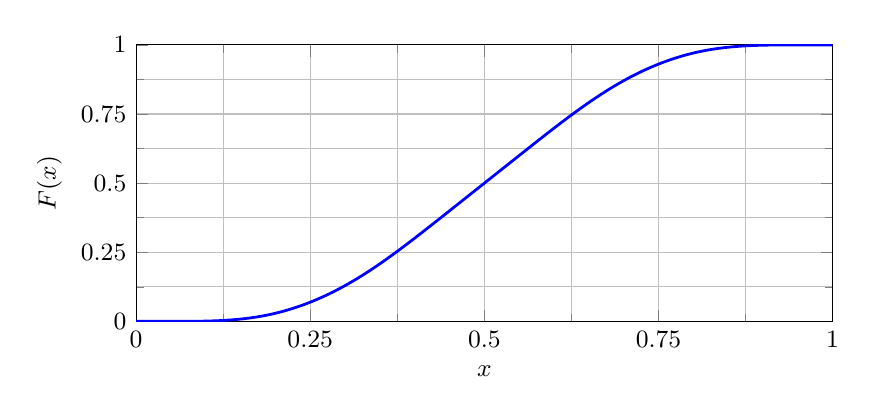
\begin{tikzpicture}
\begin{axis}[
  width=0.86\textwidth,
  height=0.42\textwidth,
  xmin=0,xmax=1,ymin=0,ymax=1,
  xlabel={$x$},ylabel={$F(x)$},
  xtick={0,0.25,0.5,0.75,1},
  ytick={0,0.25,0.5,0.75,1},
  grid=both,
  minor tick num=1,
  tick label style={font=\small},
  label style={font=\small},
]
\addplot+[mark=none,line width=1pt] coordinates {
    (0.000000000000,0.000000000000)
    (0.003906250000,0.000000000000)
    (0.007812500000,0.000000000003)
    (0.011718750000,0.000000000156)
    (0.015625000000,0.000000002052)
    (0.019531250000,0.000000013767)
    (0.023437500000,0.000000061168)
    (0.027343750000,0.000000206403)
    (0.031250000000,0.000000572676)
    (0.035156250000,0.000001372737)
    (0.039062500000,0.000002938550)
    (0.042968750000,0.000005750944)
    (0.046875000000,0.000010468114)
    (0.050781250000,0.000017950394)
    (0.054687500000,0.000029278740)
    (0.058593750000,0.000045766050)
    (0.062500000000,0.000068962191)
    (0.066406250000,0.000100655306)
    (0.070312500000,0.000142871948)
    (0.074218750000,0.000197876948)
    (0.078125000000,0.000268172107)
    (0.082031250000,0.000356491165)
    (0.085937500000,0.000465788485)
    (0.089843750000,0.000599220570)
    (0.093750000000,0.000760121287)
    (0.097656250000,0.000951973371)
    (0.101562500000,0.001178378768)
    (0.105468750000,0.001443028972)
    (0.109375000000,0.001749676531)
    (0.113281250000,0.002102110277)
    (0.117187500000,0.002504136830)
    (0.121093750000,0.002959569295)
    (0.125000000000,0.003472222222)
    (0.128906250000,0.004045910305)
    (0.132812500000,0.004684448239)
    (0.136718750000,0.005391650574)
    (0.140625000000,0.006171330413)
    (0.144531250000,0.007027294379)
    (0.148437500000,0.007963331302)
    (0.152343750000,0.008983193730)
    (0.156250000000,0.010090573158)
    (0.160156250000,0.011289071531)
    (0.164062500000,0.012582171585)
    (0.167968750000,0.013973207186)
    (0.171875000000,0.015465334837)
    (0.175781250000,0.017061508903)
    (0.179687500000,0.018764463122)
    (0.183593750000,0.020576699295)
    (0.187500000000,0.022500482253)
    (0.191406250000,0.024537838550)
    (0.195312500000,0.026690556329)
    (0.199218750000,0.028960185457)
    (0.203125000000,0.031348038830)
    (0.207031250000,0.033855197407)
    (0.210937500000,0.036482521520)
    (0.214843750000,0.039230669363)
    (0.218750000000,0.042100121769)
    (0.222656250000,0.045091210698)
    (0.226562500000,0.048204148902)
    (0.230468750000,0.051439059583)
    (0.234375000000,0.054796004892)
    (0.238281250000,0.058275010695)
    (0.242187500000,0.061876085066)
    (0.246093750000,0.065599229601)
    (0.250000000000,0.069444444444)
    (0.253906250000,0.073411729601)
    (0.257812500000,0.077501085066)
    (0.261718750000,0.081712510695)
    (0.265625000000,0.086046004892)
    (0.269531250000,0.090501559583)
    (0.273437500000,0.095079148902)
    (0.277343750000,0.099778710698)
    (0.281250000000,0.104600121769)
    (0.285156250000,0.109543169363)
    (0.289062500000,0.114607521520)
    (0.292968750000,0.119792697407)
    (0.296875000000,0.125098038830)
    (0.300781250000,0.130522685457)
    (0.304687500000,0.136065556329)
    (0.308593750000,0.141725338550)
    (0.312500000000,0.147500482253)
    (0.316406250000,0.153389199295)
    (0.320312500000,0.159389463122)
    (0.324218750000,0.165499008903)
    (0.328125000000,0.171715334837)
    (0.332031250000,0.178035707186)
    (0.335937500000,0.184457171585)
    (0.339843750000,0.190976571531)
    (0.343750000000,0.197590573158)
    (0.347656250000,0.204295693730)
    (0.351562500000,0.211088331302)
    (0.355468750000,0.217964794379)
    (0.359375000000,0.224921330413)
    (0.363281250000,0.231954150574)
    (0.367187500000,0.239059448239)
    (0.371093750000,0.246233410305)
    (0.375000000000,0.253472222222)
    (0.378906250000,0.260772069295)
    (0.382812500000,0.268129136830)
    (0.386718750000,0.275539610277)
    (0.390625000000,0.282999676531)
    (0.394531250000,0.290505528972)
    (0.398437500000,0.298053378768)
    (0.402343750000,0.305639473371)
    (0.406250000000,0.313260121287)
    (0.410156250000,0.320911720570)
    (0.414062500000,0.328590788485)
    (0.417968750000,0.336293991165)
    (0.421875000000,0.344018172107)
    (0.425781250000,0.351760376948)
    (0.429687500000,0.359517871948)
    (0.433593750000,0.367288155306)
    (0.437500000000,0.375068962191)
    (0.441406250000,0.382858266050)
    (0.445312500000,0.390654278740)
    (0.449218750000,0.398455450394)
    (0.453125000000,0.406260468114)
    (0.457031250000,0.414068250944)
    (0.460937500000,0.421877938550)
    (0.464843750000,0.429688872737)
    (0.468750000000,0.437500572676)
    (0.472656250000,0.445312706403)
    (0.476562500000,0.453125061168)
    (0.480468750000,0.460937513767)
    (0.484375000000,0.468750002052)
    (0.488281250000,0.476562500156)
    (0.492187500000,0.484375000003)
    (0.496093750000,0.492187500000)
    (0.500000000000,0.500000000000)
    (0.503906250000,0.507812500000)
    (0.507812500000,0.515624999997)
    (0.511718750000,0.523437499844)
    (0.515625000000,0.531249997948)
    (0.519531250000,0.539062486233)
    (0.523437500000,0.546874938832)
    (0.527343750000,0.554687293597)
    (0.531250000000,0.562499427324)
    (0.535156250000,0.570311127263)
    (0.539062500000,0.578122061450)
    (0.542968750000,0.585931749056)
    (0.546875000000,0.593739531886)
    (0.550781250000,0.601544549606)
    (0.554687500000,0.609345721260)
    (0.558593750000,0.617141733950)
    (0.562500000000,0.624931037809)
    (0.566406250000,0.632711844694)
    (0.570312500000,0.640482128052)
    (0.574218750000,0.648239623052)
    (0.578125000000,0.655981827893)
    (0.582031250000,0.663706008835)
    (0.585937500000,0.671409211515)
    (0.589843750000,0.679088279430)
    (0.593750000000,0.686739878713)
    (0.597656250000,0.694360526629)
    (0.601562500000,0.701946621232)
    (0.605468750000,0.709494471028)
    (0.609375000000,0.717000323469)
    (0.613281250000,0.724460389723)
    (0.617187500000,0.731870863170)
    (0.621093750000,0.739227930705)
    (0.625000000000,0.746527777778)
    (0.628906250000,0.753766589695)
    (0.632812500000,0.760940551761)
    (0.636718750000,0.768045849426)
    (0.640625000000,0.775078669587)
    (0.644531250000,0.782035205621)
    (0.648437500000,0.788911668698)
    (0.652343750000,0.795704306270)
    (0.656250000000,0.802409426842)
    (0.660156250000,0.809023428469)
    (0.664062500000,0.815542828415)
    (0.667968750000,0.821964292814)
    (0.671875000000,0.828284665163)
    (0.675781250000,0.834500991097)
    (0.679687500000,0.840610536878)
    (0.683593750000,0.846610800705)
    (0.687500000000,0.852499517747)
    (0.691406250000,0.858274661450)
    (0.695312500000,0.863934443671)
    (0.699218750000,0.869477314543)
    (0.703125000000,0.874901961170)
    (0.707031250000,0.880207302593)
    (0.710937500000,0.885392478480)
    (0.714843750000,0.890456830637)
    (0.718750000000,0.895399878231)
    (0.722656250000,0.900221289302)
    (0.726562500000,0.904920851098)
    (0.730468750000,0.909498440417)
    (0.734375000000,0.913953995108)
    (0.738281250000,0.918287489305)
    (0.742187500000,0.922498914934)
    (0.746093750000,0.926588270399)
    (0.750000000000,0.930555555556)
    (0.753906250000,0.934400770399)
    (0.757812500000,0.938123914934)
    (0.761718750000,0.941724989305)
    (0.765625000000,0.945203995108)
    (0.769531250000,0.948560940417)
    (0.773437500000,0.951795851098)
    (0.777343750000,0.954908789302)
    (0.781250000000,0.957899878231)
    (0.785156250000,0.960769330637)
    (0.789062500000,0.963517478480)
    (0.792968750000,0.966144802593)
    (0.796875000000,0.968651961170)
    (0.800781250000,0.971039814543)
    (0.804687500000,0.973309443671)
    (0.808593750000,0.975462161450)
    (0.812500000000,0.977499517747)
    (0.816406250000,0.979423300705)
    (0.820312500000,0.981235536878)
    (0.824218750000,0.982938491097)
    (0.828125000000,0.984534665163)
    (0.832031250000,0.986026792814)
    (0.835937500000,0.987417828415)
    (0.839843750000,0.988710928469)
    (0.843750000000,0.989909426842)
    (0.847656250000,0.991016806270)
    (0.851562500000,0.992036668698)
    (0.855468750000,0.992972705621)
    (0.859375000000,0.993828669587)
    (0.863281250000,0.994608349426)
    (0.867187500000,0.995315551761)
    (0.871093750000,0.995954089695)
    (0.875000000000,0.996527777778)
    (0.878906250000,0.997040430705)
    (0.882812500000,0.997495863170)
    (0.886718750000,0.997897889723)
    (0.890625000000,0.998250323469)
    (0.894531250000,0.998556971028)
    (0.898437500000,0.998821621232)
    (0.902343750000,0.999048026629)
    (0.906250000000,0.999239878713)
    (0.910156250000,0.999400779430)
    (0.914062500000,0.999534211515)
    (0.917968750000,0.999643508835)
    (0.921875000000,0.999731827893)
    (0.925781250000,0.999802123052)
    (0.929687500000,0.999857128052)
    (0.933593750000,0.999899344694)
    (0.937500000000,0.999931037809)
    (0.941406250000,0.999954233950)
    (0.945312500000,0.999970721260)
    (0.949218750000,0.999982049606)
    (0.953125000000,0.999989531886)
    (0.957031250000,0.999994249056)
    (0.960937500000,0.999997061450)
    (0.964843750000,0.999998627263)
    (0.968750000000,0.999999427324)
    (0.972656250000,0.999999793597)
    (0.976562500000,0.999999938832)
    (0.980468750000,0.999999986233)
    (0.984375000000,0.999999997948)
    (0.988281250000,0.999999999844)
    (0.992187500000,0.999999999997)
    (0.996093750000,1.000000000000)
    (1.000000000000,1.000000000000)
};
\end{axis}
\end{tikzpicture}
\caption{The bounded Fabius function on $[0,1]$, drawn through exact dyadic values on a
$2^{-8}$ grid.  At this resolution the straight segments are visually indistinguishable
from the smooth curve.}
\label{fig:fabius}
\end{figure}

\begin{figure}[htbp]
\centering
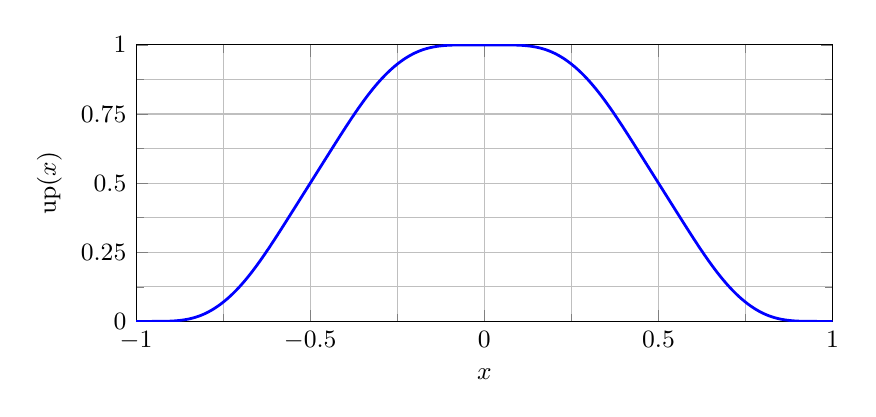
\begin{tikzpicture}
\begin{axis}[
  width=0.86\textwidth,
  height=0.42\textwidth,
  xmin=-1,xmax=1,ymin=0,ymax=1,
  xlabel={$x$},ylabel={$\Up(x)$},
  xtick={-1,-0.5,0,0.5,1},
  ytick={0,0.25,0.5,0.75,1},
  grid=both,
  minor tick num=1,
  tick label style={font=\small},
  label style={font=\small},
]
\addplot+[mark=none,line width=1pt] coordinates {
    (-1.000000000000,0.000000000000)
    (-0.996093750000,0.000000000000)
    (-0.992187500000,0.000000000003)
    (-0.988281250000,0.000000000156)
    (-0.984375000000,0.000000002052)
    (-0.980468750000,0.000000013767)
    (-0.976562500000,0.000000061168)
    (-0.972656250000,0.000000206403)
    (-0.968750000000,0.000000572676)
    (-0.964843750000,0.000001372737)
    (-0.960937500000,0.000002938550)
    (-0.957031250000,0.000005750944)
    (-0.953125000000,0.000010468114)
    (-0.949218750000,0.000017950394)
    (-0.945312500000,0.000029278740)
    (-0.941406250000,0.000045766050)
    (-0.937500000000,0.000068962191)
    (-0.933593750000,0.000100655306)
    (-0.929687500000,0.000142871948)
    (-0.925781250000,0.000197876948)
    (-0.921875000000,0.000268172107)
    (-0.917968750000,0.000356491165)
    (-0.914062500000,0.000465788485)
    (-0.910156250000,0.000599220570)
    (-0.906250000000,0.000760121287)
    (-0.902343750000,0.000951973371)
    (-0.898437500000,0.001178378768)
    (-0.894531250000,0.001443028972)
    (-0.890625000000,0.001749676531)
    (-0.886718750000,0.002102110277)
    (-0.882812500000,0.002504136830)
    (-0.878906250000,0.002959569295)
    (-0.875000000000,0.003472222222)
    (-0.871093750000,0.004045910305)
    (-0.867187500000,0.004684448239)
    (-0.863281250000,0.005391650574)
    (-0.859375000000,0.006171330413)
    (-0.855468750000,0.007027294379)
    (-0.851562500000,0.007963331302)
    (-0.847656250000,0.008983193730)
    (-0.843750000000,0.010090573158)
    (-0.839843750000,0.011289071531)
    (-0.835937500000,0.012582171585)
    (-0.832031250000,0.013973207186)
    (-0.828125000000,0.015465334837)
    (-0.824218750000,0.017061508903)
    (-0.820312500000,0.018764463122)
    (-0.816406250000,0.020576699295)
    (-0.812500000000,0.022500482253)
    (-0.808593750000,0.024537838550)
    (-0.804687500000,0.026690556329)
    (-0.800781250000,0.028960185457)
    (-0.796875000000,0.031348038830)
    (-0.792968750000,0.033855197407)
    (-0.789062500000,0.036482521520)
    (-0.785156250000,0.039230669363)
    (-0.781250000000,0.042100121769)
    (-0.777343750000,0.045091210698)
    (-0.773437500000,0.048204148902)
    (-0.769531250000,0.051439059583)
    (-0.765625000000,0.054796004892)
    (-0.761718750000,0.058275010695)
    (-0.757812500000,0.061876085066)
    (-0.753906250000,0.065599229601)
    (-0.750000000000,0.069444444444)
    (-0.746093750000,0.073411729601)
    (-0.742187500000,0.077501085066)
    (-0.738281250000,0.081712510695)
    (-0.734375000000,0.086046004892)
    (-0.730468750000,0.090501559583)
    (-0.726562500000,0.095079148902)
    (-0.722656250000,0.099778710698)
    (-0.718750000000,0.104600121769)
    (-0.714843750000,0.109543169363)
    (-0.710937500000,0.114607521520)
    (-0.707031250000,0.119792697407)
    (-0.703125000000,0.125098038830)
    (-0.699218750000,0.130522685457)
    (-0.695312500000,0.136065556329)
    (-0.691406250000,0.141725338550)
    (-0.687500000000,0.147500482253)
    (-0.683593750000,0.153389199295)
    (-0.679687500000,0.159389463122)
    (-0.675781250000,0.165499008903)
    (-0.671875000000,0.171715334837)
    (-0.667968750000,0.178035707186)
    (-0.664062500000,0.184457171585)
    (-0.660156250000,0.190976571531)
    (-0.656250000000,0.197590573158)
    (-0.652343750000,0.204295693730)
    (-0.648437500000,0.211088331302)
    (-0.644531250000,0.217964794379)
    (-0.640625000000,0.224921330413)
    (-0.636718750000,0.231954150574)
    (-0.632812500000,0.239059448239)
    (-0.628906250000,0.246233410305)
    (-0.625000000000,0.253472222222)
    (-0.621093750000,0.260772069295)
    (-0.617187500000,0.268129136830)
    (-0.613281250000,0.275539610277)
    (-0.609375000000,0.282999676531)
    (-0.605468750000,0.290505528972)
    (-0.601562500000,0.298053378768)
    (-0.597656250000,0.305639473371)
    (-0.593750000000,0.313260121287)
    (-0.589843750000,0.320911720570)
    (-0.585937500000,0.328590788485)
    (-0.582031250000,0.336293991165)
    (-0.578125000000,0.344018172107)
    (-0.574218750000,0.351760376948)
    (-0.570312500000,0.359517871948)
    (-0.566406250000,0.367288155306)
    (-0.562500000000,0.375068962191)
    (-0.558593750000,0.382858266050)
    (-0.554687500000,0.390654278740)
    (-0.550781250000,0.398455450394)
    (-0.546875000000,0.406260468114)
    (-0.542968750000,0.414068250944)
    (-0.539062500000,0.421877938550)
    (-0.535156250000,0.429688872737)
    (-0.531250000000,0.437500572676)
    (-0.527343750000,0.445312706403)
    (-0.523437500000,0.453125061168)
    (-0.519531250000,0.460937513767)
    (-0.515625000000,0.468750002052)
    (-0.511718750000,0.476562500156)
    (-0.507812500000,0.484375000003)
    (-0.503906250000,0.492187500000)
    (-0.500000000000,0.500000000000)
    (-0.496093750000,0.507812500000)
    (-0.492187500000,0.515624999997)
    (-0.488281250000,0.523437499844)
    (-0.484375000000,0.531249997948)
    (-0.480468750000,0.539062486233)
    (-0.476562500000,0.546874938832)
    (-0.472656250000,0.554687293597)
    (-0.468750000000,0.562499427324)
    (-0.464843750000,0.570311127263)
    (-0.460937500000,0.578122061450)
    (-0.457031250000,0.585931749056)
    (-0.453125000000,0.593739531886)
    (-0.449218750000,0.601544549606)
    (-0.445312500000,0.609345721260)
    (-0.441406250000,0.617141733950)
    (-0.437500000000,0.624931037809)
    (-0.433593750000,0.632711844694)
    (-0.429687500000,0.640482128052)
    (-0.425781250000,0.648239623052)
    (-0.421875000000,0.655981827893)
    (-0.417968750000,0.663706008835)
    (-0.414062500000,0.671409211515)
    (-0.410156250000,0.679088279430)
    (-0.406250000000,0.686739878713)
    (-0.402343750000,0.694360526629)
    (-0.398437500000,0.701946621232)
    (-0.394531250000,0.709494471028)
    (-0.390625000000,0.717000323469)
    (-0.386718750000,0.724460389723)
    (-0.382812500000,0.731870863170)
    (-0.378906250000,0.739227930705)
    (-0.375000000000,0.746527777778)
    (-0.371093750000,0.753766589695)
    (-0.367187500000,0.760940551761)
    (-0.363281250000,0.768045849426)
    (-0.359375000000,0.775078669587)
    (-0.355468750000,0.782035205621)
    (-0.351562500000,0.788911668698)
    (-0.347656250000,0.795704306270)
    (-0.343750000000,0.802409426842)
    (-0.339843750000,0.809023428469)
    (-0.335937500000,0.815542828415)
    (-0.332031250000,0.821964292814)
    (-0.328125000000,0.828284665163)
    (-0.324218750000,0.834500991097)
    (-0.320312500000,0.840610536878)
    (-0.316406250000,0.846610800705)
    (-0.312500000000,0.852499517747)
    (-0.308593750000,0.858274661450)
    (-0.304687500000,0.863934443671)
    (-0.300781250000,0.869477314543)
    (-0.296875000000,0.874901961170)
    (-0.292968750000,0.880207302593)
    (-0.289062500000,0.885392478480)
    (-0.285156250000,0.890456830637)
    (-0.281250000000,0.895399878231)
    (-0.277343750000,0.900221289302)
    (-0.273437500000,0.904920851098)
    (-0.269531250000,0.909498440417)
    (-0.265625000000,0.913953995108)
    (-0.261718750000,0.918287489305)
    (-0.257812500000,0.922498914934)
    (-0.253906250000,0.926588270399)
    (-0.250000000000,0.930555555556)
    (-0.246093750000,0.934400770399)
    (-0.242187500000,0.938123914934)
    (-0.238281250000,0.941724989305)
    (-0.234375000000,0.945203995108)
    (-0.230468750000,0.948560940417)
    (-0.226562500000,0.951795851098)
    (-0.222656250000,0.954908789302)
    (-0.218750000000,0.957899878231)
    (-0.214843750000,0.960769330637)
    (-0.210937500000,0.963517478480)
    (-0.207031250000,0.966144802593)
    (-0.203125000000,0.968651961170)
    (-0.199218750000,0.971039814543)
    (-0.195312500000,0.973309443671)
    (-0.191406250000,0.975462161450)
    (-0.187500000000,0.977499517747)
    (-0.183593750000,0.979423300705)
    (-0.179687500000,0.981235536878)
    (-0.175781250000,0.982938491097)
    (-0.171875000000,0.984534665163)
    (-0.167968750000,0.986026792814)
    (-0.164062500000,0.987417828415)
    (-0.160156250000,0.988710928469)
    (-0.156250000000,0.989909426842)
    (-0.152343750000,0.991016806270)
    (-0.148437500000,0.992036668698)
    (-0.144531250000,0.992972705621)
    (-0.140625000000,0.993828669587)
    (-0.136718750000,0.994608349426)
    (-0.132812500000,0.995315551761)
    (-0.128906250000,0.995954089695)
    (-0.125000000000,0.996527777778)
    (-0.121093750000,0.997040430705)
    (-0.117187500000,0.997495863170)
    (-0.113281250000,0.997897889723)
    (-0.109375000000,0.998250323469)
    (-0.105468750000,0.998556971028)
    (-0.101562500000,0.998821621232)
    (-0.097656250000,0.999048026629)
    (-0.093750000000,0.999239878713)
    (-0.089843750000,0.999400779430)
    (-0.085937500000,0.999534211515)
    (-0.082031250000,0.999643508835)
    (-0.078125000000,0.999731827893)
    (-0.074218750000,0.999802123052)
    (-0.070312500000,0.999857128052)
    (-0.066406250000,0.999899344694)
    (-0.062500000000,0.999931037809)
    (-0.058593750000,0.999954233950)
    (-0.054687500000,0.999970721260)
    (-0.050781250000,0.999982049606)
    (-0.046875000000,0.999989531886)
    (-0.042968750000,0.999994249056)
    (-0.039062500000,0.999997061450)
    (-0.035156250000,0.999998627263)
    (-0.031250000000,0.999999427324)
    (-0.027343750000,0.999999793597)
    (-0.023437500000,0.999999938832)
    (-0.019531250000,0.999999986233)
    (-0.015625000000,0.999999997948)
    (-0.011718750000,0.999999999844)
    (-0.007812500000,0.999999999997)
    (-0.003906250000,1.000000000000)
    (0.000000000000,1.000000000000)
    (0.003906250000,1.000000000000)
    (0.007812500000,0.999999999997)
    (0.011718750000,0.999999999844)
    (0.015625000000,0.999999997948)
    (0.019531250000,0.999999986233)
    (0.023437500000,0.999999938832)
    (0.027343750000,0.999999793597)
    (0.031250000000,0.999999427324)
    (0.035156250000,0.999998627263)
    (0.039062500000,0.999997061450)
    (0.042968750000,0.999994249056)
    (0.046875000000,0.999989531886)
    (0.050781250000,0.999982049606)
    (0.054687500000,0.999970721260)
    (0.058593750000,0.999954233950)
    (0.062500000000,0.999931037809)
    (0.066406250000,0.999899344694)
    (0.070312500000,0.999857128052)
    (0.074218750000,0.999802123052)
    (0.078125000000,0.999731827893)
    (0.082031250000,0.999643508835)
    (0.085937500000,0.999534211515)
    (0.089843750000,0.999400779430)
    (0.093750000000,0.999239878713)
    (0.097656250000,0.999048026629)
    (0.101562500000,0.998821621232)
    (0.105468750000,0.998556971028)
    (0.109375000000,0.998250323469)
    (0.113281250000,0.997897889723)
    (0.117187500000,0.997495863170)
    (0.121093750000,0.997040430705)
    (0.125000000000,0.996527777778)
    (0.128906250000,0.995954089695)
    (0.132812500000,0.995315551761)
    (0.136718750000,0.994608349426)
    (0.140625000000,0.993828669587)
    (0.144531250000,0.992972705621)
    (0.148437500000,0.992036668698)
    (0.152343750000,0.991016806270)
    (0.156250000000,0.989909426842)
    (0.160156250000,0.988710928469)
    (0.164062500000,0.987417828415)
    (0.167968750000,0.986026792814)
    (0.171875000000,0.984534665163)
    (0.175781250000,0.982938491097)
    (0.179687500000,0.981235536878)
    (0.183593750000,0.979423300705)
    (0.187500000000,0.977499517747)
    (0.191406250000,0.975462161450)
    (0.195312500000,0.973309443671)
    (0.199218750000,0.971039814543)
    (0.203125000000,0.968651961170)
    (0.207031250000,0.966144802593)
    (0.210937500000,0.963517478480)
    (0.214843750000,0.960769330637)
    (0.218750000000,0.957899878231)
    (0.222656250000,0.954908789302)
    (0.226562500000,0.951795851098)
    (0.230468750000,0.948560940417)
    (0.234375000000,0.945203995108)
    (0.238281250000,0.941724989305)
    (0.242187500000,0.938123914934)
    (0.246093750000,0.934400770399)
    (0.250000000000,0.930555555556)
    (0.253906250000,0.926588270399)
    (0.257812500000,0.922498914934)
    (0.261718750000,0.918287489305)
    (0.265625000000,0.913953995108)
    (0.269531250000,0.909498440417)
    (0.273437500000,0.904920851098)
    (0.277343750000,0.900221289302)
    (0.281250000000,0.895399878231)
    (0.285156250000,0.890456830637)
    (0.289062500000,0.885392478480)
    (0.292968750000,0.880207302593)
    (0.296875000000,0.874901961170)
    (0.300781250000,0.869477314543)
    (0.304687500000,0.863934443671)
    (0.308593750000,0.858274661450)
    (0.312500000000,0.852499517747)
    (0.316406250000,0.846610800705)
    (0.320312500000,0.840610536878)
    (0.324218750000,0.834500991097)
    (0.328125000000,0.828284665163)
    (0.332031250000,0.821964292814)
    (0.335937500000,0.815542828415)
    (0.339843750000,0.809023428469)
    (0.343750000000,0.802409426842)
    (0.347656250000,0.795704306270)
    (0.351562500000,0.788911668698)
    (0.355468750000,0.782035205621)
    (0.359375000000,0.775078669587)
    (0.363281250000,0.768045849426)
    (0.367187500000,0.760940551761)
    (0.371093750000,0.753766589695)
    (0.375000000000,0.746527777778)
    (0.378906250000,0.739227930705)
    (0.382812500000,0.731870863170)
    (0.386718750000,0.724460389723)
    (0.390625000000,0.717000323469)
    (0.394531250000,0.709494471028)
    (0.398437500000,0.701946621232)
    (0.402343750000,0.694360526629)
    (0.406250000000,0.686739878713)
    (0.410156250000,0.679088279430)
    (0.414062500000,0.671409211515)
    (0.417968750000,0.663706008835)
    (0.421875000000,0.655981827893)
    (0.425781250000,0.648239623052)
    (0.429687500000,0.640482128052)
    (0.433593750000,0.632711844694)
    (0.437500000000,0.624931037809)
    (0.441406250000,0.617141733950)
    (0.445312500000,0.609345721260)
    (0.449218750000,0.601544549606)
    (0.453125000000,0.593739531886)
    (0.457031250000,0.585931749056)
    (0.460937500000,0.578122061450)
    (0.464843750000,0.570311127263)
    (0.468750000000,0.562499427324)
    (0.472656250000,0.554687293597)
    (0.476562500000,0.546874938832)
    (0.480468750000,0.539062486233)
    (0.484375000000,0.531249997948)
    (0.488281250000,0.523437499844)
    (0.492187500000,0.515624999997)
    (0.496093750000,0.507812500000)
    (0.500000000000,0.500000000000)
    (0.503906250000,0.492187500000)
    (0.507812500000,0.484375000003)
    (0.511718750000,0.476562500156)
    (0.515625000000,0.468750002052)
    (0.519531250000,0.460937513767)
    (0.523437500000,0.453125061168)
    (0.527343750000,0.445312706403)
    (0.531250000000,0.437500572676)
    (0.535156250000,0.429688872737)
    (0.539062500000,0.421877938550)
    (0.542968750000,0.414068250944)
    (0.546875000000,0.406260468114)
    (0.550781250000,0.398455450394)
    (0.554687500000,0.390654278740)
    (0.558593750000,0.382858266050)
    (0.562500000000,0.375068962191)
    (0.566406250000,0.367288155306)
    (0.570312500000,0.359517871948)
    (0.574218750000,0.351760376948)
    (0.578125000000,0.344018172107)
    (0.582031250000,0.336293991165)
    (0.585937500000,0.328590788485)
    (0.589843750000,0.320911720570)
    (0.593750000000,0.313260121287)
    (0.597656250000,0.305639473371)
    (0.601562500000,0.298053378768)
    (0.605468750000,0.290505528972)
    (0.609375000000,0.282999676531)
    (0.613281250000,0.275539610277)
    (0.617187500000,0.268129136830)
    (0.621093750000,0.260772069295)
    (0.625000000000,0.253472222222)
    (0.628906250000,0.246233410305)
    (0.632812500000,0.239059448239)
    (0.636718750000,0.231954150574)
    (0.640625000000,0.224921330413)
    (0.644531250000,0.217964794379)
    (0.648437500000,0.211088331302)
    (0.652343750000,0.204295693730)
    (0.656250000000,0.197590573158)
    (0.660156250000,0.190976571531)
    (0.664062500000,0.184457171585)
    (0.667968750000,0.178035707186)
    (0.671875000000,0.171715334837)
    (0.675781250000,0.165499008903)
    (0.679687500000,0.159389463122)
    (0.683593750000,0.153389199295)
    (0.687500000000,0.147500482253)
    (0.691406250000,0.141725338550)
    (0.695312500000,0.136065556329)
    (0.699218750000,0.130522685457)
    (0.703125000000,0.125098038830)
    (0.707031250000,0.119792697407)
    (0.710937500000,0.114607521520)
    (0.714843750000,0.109543169363)
    (0.718750000000,0.104600121769)
    (0.722656250000,0.099778710698)
    (0.726562500000,0.095079148902)
    (0.730468750000,0.090501559583)
    (0.734375000000,0.086046004892)
    (0.738281250000,0.081712510695)
    (0.742187500000,0.077501085066)
    (0.746093750000,0.073411729601)
    (0.750000000000,0.069444444444)
    (0.753906250000,0.065599229601)
    (0.757812500000,0.061876085066)
    (0.761718750000,0.058275010695)
    (0.765625000000,0.054796004892)
    (0.769531250000,0.051439059583)
    (0.773437500000,0.048204148902)
    (0.777343750000,0.045091210698)
    (0.781250000000,0.042100121769)
    (0.785156250000,0.039230669363)
    (0.789062500000,0.036482521520)
    (0.792968750000,0.033855197407)
    (0.796875000000,0.031348038830)
    (0.800781250000,0.028960185457)
    (0.804687500000,0.026690556329)
    (0.808593750000,0.024537838550)
    (0.812500000000,0.022500482253)
    (0.816406250000,0.020576699295)
    (0.820312500000,0.018764463122)
    (0.824218750000,0.017061508903)
    (0.828125000000,0.015465334837)
    (0.832031250000,0.013973207186)
    (0.835937500000,0.012582171585)
    (0.839843750000,0.011289071531)
    (0.843750000000,0.010090573158)
    (0.847656250000,0.008983193730)
    (0.851562500000,0.007963331302)
    (0.855468750000,0.007027294379)
    (0.859375000000,0.006171330413)
    (0.863281250000,0.005391650574)
    (0.867187500000,0.004684448239)
    (0.871093750000,0.004045910305)
    (0.875000000000,0.003472222222)
    (0.878906250000,0.002959569295)
    (0.882812500000,0.002504136830)
    (0.886718750000,0.002102110277)
    (0.890625000000,0.001749676531)
    (0.894531250000,0.001443028972)
    (0.898437500000,0.001178378768)
    (0.902343750000,0.000951973371)
    (0.906250000000,0.000760121287)
    (0.910156250000,0.000599220570)
    (0.914062500000,0.000465788485)
    (0.917968750000,0.000356491165)
    (0.921875000000,0.000268172107)
    (0.925781250000,0.000197876948)
    (0.929687500000,0.000142871948)
    (0.933593750000,0.000100655306)
    (0.937500000000,0.000068962191)
    (0.941406250000,0.000045766050)
    (0.945312500000,0.000029278740)
    (0.949218750000,0.000017950394)
    (0.953125000000,0.000010468114)
    (0.957031250000,0.000005750944)
    (0.960937500000,0.000002938550)
    (0.964843750000,0.000001372737)
    (0.968750000000,0.000000572676)
    (0.972656250000,0.000000206403)
    (0.976562500000,0.000000061168)
    (0.980468750000,0.000000013767)
    (0.984375000000,0.000000002052)
    (0.988281250000,0.000000000156)
    (0.992187500000,0.000000000003)
    (0.996093750000,0.000000000000)
    (1.000000000000,0.000000000000)
};
\end{axis}
\end{tikzpicture}
\caption{Rvachev's $\Up$-function on its support $[-1,1]$, obtained by folding the same
exact dyadic data.}
\label{fig:up}
\end{figure}

\subsection{The signed global extension}

Let $\wt(n)$ denote the sum of the binary digits of $n$, and put
\begin{equation}
 \varepsilon_n=(-1)^{\wt(n)}.                             \label{eq:tm-sign}
\end{equation}
The sequence $(\varepsilon_n)$ is the $\{\pm1\}$ form of the Thue--Morse sequence
\cite{allouche2003}.

\begin{definition}[Signed extension]
Define
\begin{equation}
 \mathcal F(x)=\sum_{n\ge0}\varepsilon_n\,
   \Up(x-2n-1).                                            \label{eq:global-extension}
\end{equation}
\end{definition}

At a fixed $x$ only finitely many summands can be nonzero, so this is a locally finite sum.
On every block $[2b,2b+2]$ there is exactly one nonzero translate:
\begin{equation}
 \mathcal F(x)=\varepsilon_b\Up(x-2b-1),
 \qquad 2b\le x\le 2b+2.                                  \label{eq:single-block}
\end{equation}
It vanishes for $x\le0$, and it agrees with the bounded $F$ on $[0,1]$.  It does
\emph{not} remain in $[0,1]$ to the right of that interval.  This is the global object that
satisfies the cleanest differential equation:
\begin{equation}
 \mathcal F'(x)=2\mathcal F(2x)\qquad(x\in\R).             \label{eq:global-diffeq}
\end{equation}
Arias de Reyna's arithmetic paper uses this extension.  Statements about its values outside
$[0,1]$ must therefore not be transferred blindly to the bounded cumulative distribution.

\begin{boxedremark}
\textbf{Notation used in this article.}
$F$ always means the bounded distribution function; $\Up$ always means the compactly
supported even bump; and $\mathcal F$ always means the signed global extension.  On
$[0,1]$ we have $F=\mathcal F$, but globally they are different functions.
\end{boxedremark}

\subsection{Exact shape: positivity, bijectivity, and unimodality}
\label{shape:basic}

The three defining equations \eqref{eq:F-left}--\eqref{eq:F-diffeq} already determine the
qualitative picture, but the statements that are actually used later are the sharp ones: not
$F\ge0$ but $F(x)>0$ exactly for $x>0$; not $\Up\le1$ but $\Up(x)=1$ exactly at the origin.
We record them here, in the form of equivalences, because the strict versions are what make
the convexity and Lipschitz theorems below sharp.

Everything rests on a single formula that merges \eqref{eq:F-diffeq} and
\eqref{eq:F-diffeq-right} into one identity valid on the whole line.

\begin{lemma}[Unified derivative formula]
\label{thm:shape-unified-derivative}
For every real $x$,
\begin{equation}
 F'(x)=2\Up(2x-1).                                        \label{eq:shape-unified-derivative}
\end{equation}
\end{lemma}

\begin{proof}
By \eqref{eq:up-absolute}, $\Up(2x-1)=F\bigl(1-|2x-1|\bigr)$.  For $0\le x\le\tfrac12$ one has
$|2x-1|=1-2x$, so $\Up(2x-1)=F(2x)$ and \eqref{eq:shape-unified-derivative} is
\eqref{eq:F-diffeq}.  For $\tfrac12\le x\le1$ one has $|2x-1|=2x-1$, so $\Up(2x-1)=F(2-2x)$
and \eqref{eq:shape-unified-derivative} is \eqref{eq:F-diffeq-right}.  For $x<0$ or $x>1$ one
has $|2x-1|>1$, hence $1-|2x-1|<0$ and $\Up(2x-1)=0$ by \eqref{eq:F-left}, while $F'(x)=0$
because $F$ is constant on each exterior half-line by \eqref{eq:F-left} and
\eqref{eq:F-right}.
\end{proof}

Since $\Up\ge0$, formula \eqref{eq:shape-unified-derivative} shows at once that $F$ is
nondecreasing on all of $\R$.  It is also convenient to note that the reflection symmetry
\eqref{eq:F-symmetry}, stated on the unit interval, in fact holds globally:
\begin{equation}
 F(1-x)=1-F(x)\qquad(x\in\R).                             \label{eq:shape-symmetry-global}
\end{equation}
Indeed, for $x<0$ both sides equal $1$ by \eqref{eq:F-left} and \eqref{eq:F-right}, and for
$x>1$ both sides equal $0$.

\begin{theorem}[Positivity, strict monotonicity, bijectivity]
\label{thm:shape-bijection}
The bounded Fabius function satisfies the following.
\begin{enumerate}
\item $F(x)>0$ if and only if $x>0$.
\item $F(x)<1$ if and only if $x<1$.
\item $F'(x)>0$ for $0<x<1$, and $F$ is strictly increasing on $[0,1]$.
\item $F$ maps $[0,1]$ bijectively onto $[0,1]$.
\end{enumerate}
\end{theorem}

\begin{proof}
The heart of the matter is the following doubling step: if $0\le x\le\tfrac12$ and $F(x)=0$,
then $F(2x)=0$.  To see it, observe that $F\ge0$ everywhere, so a zero of $F$ is a global
minimum of a function differentiable on all of $\R$; Fermat's rule gives $F'(x)=0$, and
\eqref{eq:F-diffeq} turns this into $2F(2x)=0$.

Suppose now that $F(x)=0$ for some $x>0$.  Since $2^nx\to\infty$, there is a smallest
integer $n\ge0$ with $2^nx\ge\tfrac12$.  For $0\le m<n$ we have $2^mx<\tfrac12$, so the
doubling step applies at $2^mx$ and propagates the vanishing: from $F(x)=0$ we obtain
$F(2^mx)=0$ for every $m\le n$, and in particular $F(2^nx)=0$.  But $F$ is nondecreasing and
$2^nx\ge\tfrac12$, so $F(2^nx)\ge F(\tfrac12)=\tfrac12$, where the midpoint value comes from
\eqref{eq:F-symmetry} at $x=\tfrac12$.  This contradiction proves that $F$ has no zero on the
positive half-line; combined with \eqref{eq:F-left} it proves (i).

Assertion (ii) follows from (i) and \eqref{eq:shape-symmetry-global}: $F(x)<1$ if and only if
$F(1-x)>0$, that is, if and only if $1-x>0$.

For (iii), let $0<x<1$.  Then $2x-1\in(-1,1)$, so $1-|2x-1|\in(0,1]$, and (i) gives
$\Up(2x-1)=F(1-|2x-1|)>0$.  Now \eqref{eq:shape-unified-derivative} yields $F'(x)>0$.  A
continuous function on $[0,1]$ whose derivative is positive throughout the interior is
strictly increasing on $[0,1]$.

For (iv), $F$ is continuous with $F(0)=0$ and $F(1)=1$, so the intermediate value theorem
makes $F([0,1])$ contain $[0,1]$; since $F$ takes values in $[0,1]$, the image is exactly
$[0,1]$.  Strict monotonicity from (iii) gives injectivity.
\end{proof}

The fold \eqref{eq:up-absolute} now transfers the whole picture to Rvachev's bump, and it
does so in strict form.

\begin{theorem}[Strict unimodality of $\Up$]
\label{thm:shape-unimodal}
Rvachev's function satisfies the following.
\begin{enumerate}
\item $\Up$ is strictly increasing on $[-1,0]$ and strictly decreasing on $[0,1]$.
\item $\Up(x)=1$ if and only if $x=0$; the maximum value $1$ is attained at the origin and
      nowhere else.
\item $\Up(x)=0$ if and only if $x\notin(-1,1)$.  Thus $\Up$ is nonzero exactly on
      $(-1,1)$, and $\supp\Up=[-1,1]$.
\item $\Up'(x)>0$ for $-1<x<0$ and $\Up'(x)<0$ for $0<x<1$.
\end{enumerate}
\end{theorem}

\begin{proof}
By \eqref{eq:up-absolute}, $\Up(x)=F(1-x)$ for $x\ge0$.  As $x$ increases through $[0,1]$ the
argument $1-x$ decreases through $[0,1]$, on which $F$ is strictly increasing by
\cref{thm:shape-bijection}(iii); hence $\Up$ is strictly decreasing on $[0,1]$, and evenness
gives (i) on $[-1,0]$.

For (ii), $\Up(x)=F(1-|x|)$ and \cref{thm:shape-bijection}(ii) say that $\Up(x)<1$ unless
$1-|x|\ge1$, that is, unless $x=0$; and $\Up(0)=F(1)=1$.  For (iii), $\Up(x)>0$ if and only
if $1-|x|>0$ by \cref{thm:shape-bijection}(i), and $\Up\ge0$, so the zero set is exactly the
complement of $(-1,1)$; the closed support is the closure $[-1,1]$.

For (iv), the identity $\Up(x)=F(1-x)$ holds on the whole open half-line $x>0$, hence may be
differentiated there: $\Up'(x)=-F'(1-x)$, which is negative for $0<x<1$ by
\cref{thm:shape-bijection}(iii).  Evenness gives $\Up'(x)=-\Up'(-x)$, so $\Up'>0$ on
$(-1,0)$.
\end{proof}

Parts (i) and (iii) are the classical description of the bump \cite{rvachev1990,arias1982};
the strict forms, and the equivalences in \cref{thm:shape-bijection}, are exactly what the
formal development records.

\subsection{Convexity and the unique inflection point}
\label{shape:convexity}

Formula \eqref{eq:shape-unified-derivative} converts the first-order shape of $\Up$ into the
second-order shape of $F$.  The affine substitution $x\mapsto2x-1$ carries
$(-\infty,\tfrac12]$ onto $(-\infty,0]$ and $[\tfrac12,\infty)$ onto $[0,\infty)$, which are
precisely the two halves on which $\Up$ is monotone.

\begin{theorem}[Convexity and the inflection point]
\label{thm:shape-convexity}
The derivative $F'$ is nondecreasing on $(-\infty,\tfrac12]$ and nonincreasing on
$[\tfrac12,\infty)$, and it is strictly increasing on $[0,\tfrac12]$ and strictly decreasing
on $[\tfrac12,1]$.  Consequently $F$ is convex on $(-\infty,\tfrac12]$ and concave on
$[\tfrac12,\infty)$, strictly convex on $[0,\tfrac12]$ and strictly concave on
$[\tfrac12,1]$.  The midpoint $x=\tfrac12$ is the unique inflection point, and
\begin{equation}
 F'(\tfrac12)=2=\max_{x\in\R}F'(x),                       \label{eq:shape-max-slope}
\end{equation}
the maximum being attained at $x=\tfrac12$ and nowhere else.
\end{theorem}

\begin{proof}
By \cref{thm:shape-unimodal}, $\Up$ is nondecreasing on $(-\infty,0]$: it vanishes on
$(-\infty,-1]$ and increases strictly on $[-1,0]$.  Symmetrically it is nonincreasing on
$[0,\infty)$.  Composing with $x\mapsto2x-1$ and using
\eqref{eq:shape-unified-derivative} shows that $F'$ is nondecreasing on $(-\infty,\tfrac12]$
and nonincreasing on $[\tfrac12,\infty)$.  If $0\le x<y\le\tfrac12$ then
$-1\le2x-1<2y-1\le0$ and the increase of $\Up$ on $[-1,0]$ is strict, so $F'(x)<F'(y)$;
the second half is symmetric.

A differentiable function on an interval is convex precisely when its derivative is
nondecreasing there, and strictly convex when the derivative is strictly increasing; the
concave statements are the same assertions for $-F$.  The intervals of strictness cannot be
enlarged: $F$ vanishes identically on $(-\infty,0]$ and equals $1$ identically on
$[1,\infty)$, so it is affine, hence not strictly convex or concave, on either exterior
half-line.

Since $F$ is convex on the whole of $(-\infty,\tfrac12]$ and concave on the whole of
$[\tfrac12,\infty)$, the sense of convexity can change only at the midpoint, and it does
change there, because $F$ is strictly convex immediately to the left of $\tfrac12$ and
strictly concave immediately to the right.  So $\tfrac12$ is the unique inflection point.
Finally $F'(x)=2\Up(2x-1)\le2\Up(0)=2$ by \cref{thm:shape-unimodal}(ii), with equality if and
only if $2x-1=0$.
\end{proof}

Differentiating \eqref{eq:shape-unified-derivative} once more gives $F''(x)=4\Up'(2x-1)$, so
$F''(\tfrac12)=4\Up'(0)=0$: the origin is an interior maximum of the differentiable function
$\Up$.  Together with $F(\tfrac12)=\tfrac12$ this locates the steepest point of the sigmoid
exactly at its centre of symmetry, where the graph crosses its own midpoint with slope $2$.

\subsection{The optimal Lipschitz constant}
\label{shape:lipschitz}

The bound $F'\le2$ of \eqref{eq:shape-max-slope} is a Lipschitz estimate, and because the
bound is attained the estimate cannot be improved.

\begin{theorem}[Two is the least Lipschitz constant]
\label{thm:shape-lipschitz}
Both $F$ and $\Up$ are $2$-Lipschitz on $\R$:
\begin{equation}
 |F(x)-F(y)|\le2|x-y|,\qquad |\Up(x)-\Up(y)|\le2|x-y|\qquad(x,y\in\R).
                                                          \label{eq:shape-lipschitz}
\end{equation}
Moreover $2$ is the least admissible constant for each: if $K\ge0$ is such that
$|F(x)-F(y)|\le K|x-y|$ for all $x,y$, or such that $|\Up(x)-\Up(y)|\le K|x-y|$ for all
$x,y$, then $K\ge2$.
\end{theorem}

\begin{proof}
By \eqref{eq:shape-unified-derivative} and $0\le\Up\le1$ we have $0\le F'\le2$ on all of
$\R$, so the mean value theorem gives the first estimate in \eqref{eq:shape-lipschitz}.  The
map $x\mapsto1-|x|$ is $1$-Lipschitz, so the second estimate follows from the first through
the fold \eqref{eq:up-absolute}.

For optimality, let $K$ be admissible for $F$.  Dividing $|F(x)-F(\tfrac12)|\le K|x-\tfrac12|$
by $|x-\tfrac12|$ and letting $x\to\tfrac12$ gives $K\ge|F'(\tfrac12)|=2$ by
\eqref{eq:shape-max-slope}.  For $\Up$ the same limit at the same point works: the proof of
\cref{thm:shape-unimodal}(iv) gives $\Up'(\tfrac12)=-F'(\tfrac12)=-2$, so $K\ge2$.
\end{proof}

The two extremal points are the same point in the two pictures: $\tfrac12$ is the centre of
the sigmoid and the midpoint of the decreasing half of the bump, and the fold sends one to
the other.

\begin{corollary}[Linear majorants at the endpoints]
\label{thm:shape-majorants}
For all admissible arguments,
\begin{align}
 F(x)&\le2x                       &&(x\ge0),   \label{eq:shape-majorant-left}\\
 1-F(x)&\le2(1-x)                 &&(x\le1),   \label{eq:shape-majorant-right}\\
 \Up(x)&\le2\bigl(1-|x|\bigr)     &&(|x|\le1). \label{eq:shape-majorant-up}
\end{align}
\end{corollary}

\begin{proof}
Applying \eqref{eq:shape-lipschitz} with $y=0$ and using $F(0)=0$ gives
\eqref{eq:shape-majorant-left}.  Replacing $x$ by $1-x$ there and using
\eqref{eq:shape-symmetry-global} gives \eqref{eq:shape-majorant-right}.  Substituting
$1-|x|\ge0$ into \eqref{eq:shape-majorant-left} and using \eqref{eq:up-absolute} gives
\eqref{eq:shape-majorant-up}.
\end{proof}

The content of \eqref{eq:shape-majorant-left} lies on $[0,\tfrac12]$; for $x\ge\tfrac12$ it is
weaker than $F\le1$.  Its value is that it holds with no hypothesis at all on the size of
$x$, so it can be used as a linear majorant in any estimate near the left endpoint, and
\eqref{eq:shape-majorant-up} says that the bump vanishes at least linearly at both ends of
its support.  These majorants and the optimality of the constant $2$ are contributions of the
formal development; the plain $2$-Lipschitz bound is used implicitly throughout
\cite{arias1982,rvachev1990}.

\section{Existence and uniqueness by a contraction}
\label{sec:existence}

The most economical construction of $F$ is a Banach fixed-point argument.  It has an
additional advantage: the contraction estimate later gives a clean uniqueness theorem,
without presupposing Fourier analysis or probability.

\subsection{The admissible function space}

Let $I=[0,1]$ and let $C(I)$ carry the supremum norm.  Define $\mathcal A\subset C(I)$ by
\begin{equation}
 \mathcal A=\{f\in C(I):0\le f\le1,
   \ f(1-x)=1-f(x)\}.                                     \label{eq:admissible-space}
\end{equation}
The set $\mathcal A$ is closed in the Banach space $C(I)$, hence complete.  It is nonempty;
for example $f(x)=x$ belongs to it.

Extend $f\in\mathcal A$ to a continuous function $\widetilde f$ on $\R$ by clamping the
argument to $I$:
\begin{equation}
 \widetilde f(t)=
 \begin{cases}
  f(0),&t\le0,\\
  f(t),&0\le t\le1,\\
  f(1),&t\ge1.
 \end{cases}                                               \label{eq:clamped-extension}
\end{equation}
Symmetry gives
\begin{equation}
 \int_0^1 f(t)\dd t=\frac12.                              \label{eq:admissible-half-integral}
\end{equation}
Indeed, replacing $t$ by $1-t$ and adding the two integrals gives $2\int_0^1f=1$.

\subsection{The integral transform}

For $f\in\mathcal A$, define $Tf$ by
\begin{equation}
 (Tf)(x)=
 \begin{cases}
  \displaystyle\int_0^{2x}\widetilde f(t)\dd t,
       &0\le x\le\tfrac12,\\[1.2ex]
  \displaystyle 1-\int_0^{2-2x}\widetilde f(t)\dd t,
       &\tfrac12<x\le1.
 \end{cases}                                               \label{eq:fixed-transform}
\end{equation}
The two definitions agree at $x=1/2$ by
\eqref{eq:admissible-half-integral}.  Positivity and the upper bound $f\le1$ show that
$0\le Tf\le1$, and a direct substitution shows $(Tf)(1-x)=1-(Tf)(x)$.  Hence
$T:\mathcal A\to\mathcal A$.

The central estimate is stronger than the naive integral bound.

\begin{lemma}[Contraction estimate]
For $f,g\in\mathcal A$,
\begin{equation}
 \|Tf-Tg\|_\infty\le\frac12\|f-g\|_\infty.                \label{eq:contraction}
\end{equation}
\end{lemma}

\begin{proof}
Write $h=f-g$.  Since both $f$ and $g$ have integral $1/2$,
$\int_0^1h=0$.  For $0\le y\le1$ we may therefore estimate the primitive in two ways:
\begin{align*}
 \left|\int_0^y h(t)\dd t\right|
 &\le y\|h\|_\infty,\\
 \left|\int_0^y h(t)\dd t\right|
 &=\left|\int_y^1h(t)\dd t\right|
 \le(1-y)\|h\|_\infty.
\end{align*}
Consequently
\begin{equation*}
 \left|\int_0^yh(t)\dd t\right|
 \le\min(y,1-y)\|h\|_\infty\le\frac12\|h\|_\infty.
\end{equation*}
Every value of $Tf-Tg$ is one of these primitives, possibly with a minus sign.  Taking the
supremum proves \eqref{eq:contraction}.
\end{proof}

\begin{theorem}[Existence of the bounded Fabius function]
The transform $T$ has a unique fixed point $f_\ast\in\mathcal A$.  Extending $f_\ast$ by
$0$ on $(-\infty,0]$ and by $1$ on $[1,\infty)$ produces the bounded Fabius function $F$.
\end{theorem}

\begin{proof}
The space $\mathcal A$ is complete and $T$ is a strict contraction with constant $1/2$, so
Banach's fixed-point theorem gives a unique fixed point.  On $[0,1/2]$ its fixed-point
equation is
\begin{equation}
 F(x)=\int_0^{2x}F(t)\dd t.                               \label{eq:F-integral-equation}
\end{equation}
Differentiating gives $F'(x)=2F(2x)$.  The second half of
\eqref{eq:fixed-transform} supplies symmetry and the matching right-hand formula.  The
endpoint values are immediate.
\end{proof}

Starting from any admissible $f_0$, the iterates $f_{n+1}=Tf_n$ converge uniformly to $F$,
with the explicit estimate
\begin{equation}
 \|f_n-F\|_\infty\le 2^{-n}\|f_0-F\|_\infty.             \label{eq:fixed-iteration-rate}
\end{equation}
This gives a conceptually simple approximation scheme, although exact dyadic evaluation will
be much faster.

\subsection{The differential equation for $\Up$ and smoothness}

Folding \eqref{eq:F-diffeq} and \eqref{eq:F-diffeq-right} yields the refinement-type
differential equation
\begin{equation}
 \Up'(x)=2\bigl(\Up(2x+1)-\Up(2x-1)\bigr)\qquad(x\in\R).  \label{eq:up-diffeq}
\end{equation}
At $x=0$ the two one-sided derivatives glue because $\Up(1)=\Up(-1)=0$.  Once $\Up$ is
continuously differentiable, \eqref{eq:up-diffeq} bootstraps regularity: if $\Up\in C^r$,
then the right side is $C^r$, so $\Up\in C^{r+1}$.  Induction gives $\Up\in C^\infty$ and
then $F\in C^\infty$.

\begin{proposition}[Basic shape]
The functions $F$ and $\Up$ have the following properties.
\begin{enumerate}
\item $F$ is strictly increasing on $(0,1)$ and satisfies $0<F(x)<1$ there.
\item $\Up$ is even, strictly positive on $(-1,1)$, and zero outside $[-1,1]$.
\item $\int_{-1}^{1}\Up(x)\dd x=1$.
\item Every derivative of $\Up$ vanishes at $x=\pm1$.
\end{enumerate}
\end{proposition}

\begin{proof}
For $0<x\le1/2$, \eqref{eq:F-diffeq} gives $F'(x)=2F(2x)$.  Positivity follows first near
$1/2$ from $F(1/2)=1/2$, and then propagates toward zero by repeatedly doubling the
argument; symmetry handles the right half.  This proves strict monotonicity and, by
\eqref{eq:up-absolute}, positivity of $\Up$ in the interior of its support.  Finally,
\begin{equation*}
 \int_{-1}^{1}\Up(x)\dd x
 =2\int_0^1F(t)\dd t=1,
\end{equation*}
where the middle identity uses the fold and the last uses symmetry.  Flatness at the support
endpoints follows from smoothness and the fact that $\Up$ is identically zero just outside
the support.
\end{proof}

\subsection{The original Rvachev characterization}

The preceding construction is equivalent to the characterization historically associated
with Rvachev.

\begin{theorem}[Original characterization]
There is a unique nonzero $C^\infty$ function $\varphi:\R\to\R$ such that
\begin{equation}
 \supp\varphi=[-1,1],\qquad
 \int_\R\varphi(x)\dd x=1,                                \label{eq:original-normalization}
\end{equation}
and
\begin{equation}
 \varphi'(x)=k\bigl(\varphi(2x+1)-\varphi(2x-1)\bigr)       \label{eq:original-rvachev}
\end{equation}
for some real scale $k$.  Necessarily $k=2$, and $\varphi=\Up$.
\end{theorem}

\begin{proofidea}
Integrating \eqref{eq:original-rvachev} against suitable test functions, or taking its
Fourier transform, first forces $k=2$ under the normalization
\eqref{eq:original-normalization}.  With the Fourier convention
\begin{equation}
 \widehat\varphi(z)=\int_\R\varphi(x)\e^{-2\pi\ii xz}\dd x,
\end{equation}
one obtains
\begin{equation}
 \widehat\varphi(z)=\sinc(\pi z)\widehat\varphi(z/2),
 \qquad \sinc z=\begin{cases}\sin z/z,&z\ne0,\\1,&z=0.\end{cases} \label{eq:fourier-refinement-preview}
\end{equation}
Iterating $N$ times gives a finite sinc product multiplied by
$\widehat\varphi(z/2^N)$.  Continuity and $\widehat\varphi(0)=1$ determine the Fourier
transform uniquely in the limit.  Fourier inversion then determines $\varphi$.  The function
constructed above satisfies all the hypotheses, so it is that unique solution.
\end{proofidea}

\section{The probability law behind the functions}
\label{sec:probability}

The fixed-point construction is analytic.  A probabilistic construction explains the same
self-similarity almost without calculation and makes monotonicity and positivity transparent.

\subsection{An infinite weighted sum of uniforms}

Let $U_0,U_1,\ldots$ be independent random variables, each uniformly distributed on
$[0,1]$, and define
\begin{equation}
 X=\sum_{n=0}^{\infty}\frac{U_n}{2^{n+1}}.                \label{eq:random-X}
\end{equation}
The series converges absolutely for every outcome and satisfies $0\le X\le1$.  Removing the
first coordinate gives an independent copy $X'$ of $X$, and
\begin{equation}
 X=\frac{U_0+X'}2.                                         \label{eq:random-split}
\end{equation}
Reflecting every coordinate, $U_n\mapsto1-U_n$, preserves the product measure and sends
$X$ to $1-X$.

Let $H(x)=\Prob(X\le x)$ be the cumulative distribution function.  Conditioning on $U_0$
in \eqref{eq:random-split} gives
\begin{equation}
 H(y)=\int_0^1 H(2y-u)\dd u.                               \label{eq:CDF-smoothing}
\end{equation}
For $0\le y\le1/2$, the integrand vanishes when $u>2y$, so
\begin{equation}
 H(y)=\int_0^{2y}H(t)\dd t.                                \label{eq:CDF-left}
\end{equation}
Reflection gives $H(1-y)=1-H(y)$.  Thus the restriction of $H$ to $[0,1]$ is a fixed point
of the contraction $T$ from \cref{sec:existence}.

\begin{theorem}[Probabilistic representation]
For every $x\in\R$,
\begin{equation}
 F(x)=\Prob\left(\sum_{n=0}^{\infty}\frac{U_n}{2^{n+1}}\le x\right). \label{eq:F-CDF}
\end{equation}
For $-1\le y\le0$,
\begin{equation}
 \Up(y)=\Prob(X\le y+1).                                  \label{eq:up-left-prob}
\end{equation}
\end{theorem}

\begin{proof}
The preceding calculation shows that $H$ is an admissible fixed point of $T$.  Uniqueness of
the fixed point gives $H=F$.  Equation \eqref{eq:up-left-prob} is then just the left branch
of \eqref{eq:up-fold}.
\end{proof}

The more symmetric random variable is
\begin{equation}
 Y=2X-1=\sum_{n=0}^{\infty}\frac{V_n}{2^{n+1}},
 \qquad V_n=2U_n-1\sim\operatorname{Unif}[-1,1].           \label{eq:random-Y}
\end{equation}
The density of $Y$ is precisely $\Up$.  Indeed, for $-1<y<1$,
\begin{equation}
 f_Y(y)=\frac12F'\!\left(\frac{y+1}{2}\right)=\Up(y).     \label{eq:up-density}
\end{equation}
This identity is a compact way to remember why $\Up$ integrates to one.

\subsection{Finite convolutions and step approximants}

For each $n$, the summand $V_n/2^{n+1}$ is uniform on
$[-2^{-n-1},2^{-n-1}]$ and has density
\begin{equation}
 b_n(x)=2^n\,\mathbf 1_{[-2^{-n-1},2^{-n-1}]}(x).          \label{eq:box-density}
\end{equation}
Hence the partial sum
\begin{equation}
 Y_N=\sum_{n=0}^{N}\frac{V_n}{2^{n+1}}
\end{equation}
has density
\begin{equation}
 u_N=b_0*b_1*\cdots*b_N.                                  \label{eq:finite-convolution}
\end{equation}
These compactly supported piecewise-polynomial densities converge to $\Up$.  Weak convergence
is immediate from almost-sure convergence of $Y_N$; the refinement equation and uniform
bounds upgrade the convergence to the strong forms used in the formal development.  This
constructs $\Up$ as an infinite convolution of shrinking boxes, a perspective useful in
approximation theory and wavelet analysis.

\subsection{Centered finite splines and an explicit error bound}
\label{sec:centered-splines}

The preceding finite random sums also give a completely explicit polynomial approximation
to $F$.  Put
\begin{equation}
 T_p=\sum_{i=0}^{p-1}\frac{U_i}{2^{i+1}},
 \qquad
 C_p(x)=\Prob\left(T_p\le x-2^{-p-1}\right),               \label{eq:centered-partial-cdf}
\end{equation}
where $p\ge1$.  The shift by half of the omitted tail is important: it centers the
one-sided approximation and improves its error by a factor of two.

Let
\begin{equation}
 N_p(x)=\max\left(0,\left\lfloor 2^p x+\frac12\right\rfloor\right),
 \qquad \varepsilon_r=(-1)^{\wt(r)},                       \label{eq:centered-cutoff}
\end{equation}
and interpret a sum with $N_p(x)=0$ as empty.  Define
\begin{equation}
 S_p(x)=
 \frac{(-1)^p}{2^{\binom p2}p!}
 \sum_{r=0}^{N_p(x)-1}
 \varepsilon_r
 \left(r-2^p x+\frac12\right)^p.                          \label{eq:centered-spline}
\end{equation}
Equivalently,
\begin{equation}
 S_p(x)=
 \frac{1}{2^{\binom p2}p!}
 \sum_{r\ge0}\varepsilon_r
 \left(2^p x-\frac12-r\right)_+^p,                        \label{eq:centered-spline-positive}
\end{equation}
where only the terms $r<N_p(x)$ can be nonzero and $t_+=\max(t,0)$.
The cutoff in \eqref{eq:centered-cutoff} is a safe natural-number form of the
inclusive upper limit
\[
 0\le r\le\left\lfloor2^p x-\frac12\right\rfloor.
\]
It handles the empty case without assigning a negative upper endpoint to a finite sum.

\begin{theorem}[Centered spline as a finite distribution function]
\label{thm:centered-spline-cdf}
For $p\ge1$ and $0\le x\le1$,
\begin{equation}
 S_p(x)=C_p(x).                                            \label{eq:spline-equals-cdf}
\end{equation}
Consequently $0\le S_p(x)\le1$ on the unit interval.
\end{theorem}

\begin{proof}
For $p=1$, $T_1=U_0/2$, and direct evaluation gives
\[
 C_1(x)=\max\left(0,\min\left(1,2x-\frac12\right)\right).
\]
Formula \eqref{eq:centered-spline-positive} gives exactly the same broken-linear
function: the term $r=0$ starts at $x=1/4$, and the term $r=1$ subtracts the excess
after $x=3/4$.

For the induction step, split off the first uniform coordinate.  The finite sums satisfy
\[
 T_{p+1}\ \overset{\mathrm d}=\ \frac{U_0+T_p'}2,
\]
where $T_p'$ is an independent copy of $T_p$.  Conditioning on $U_0$ and accounting for
the midpoint shifts gives the exact smoothing recurrence
\begin{equation}
 C_{p+1}(x)=\int_0^1 C_p(2x-u)\dd u.                      \label{eq:centered-cdf-smoothing}
\end{equation}
On the spline side, integrate each truncated power in
\eqref{eq:centered-spline-positive}.  The two binary children $2r$ and $2r+1$
have opposite Thue--Morse signs, because
\(\varepsilon_{2r}=\varepsilon_r\) and
\(\varepsilon_{2r+1}=-\varepsilon_r\).  After the change of scale this yields
\begin{equation}
 S_{p+1}(x)=\int_0^1 S_p(2x-u)\dd u.                      \label{eq:centered-spline-smoothing}
\end{equation}
The normalization is exactly the one required by
\[
 \sum_{r=0}^{2^p-1}\varepsilon_r r^p
 =(-1)^p2^{\binom p2}p!,
\]
while every lower power sum vanishes.  Thus the two recurrences and their common base
case prove \eqref{eq:spline-equals-cdf}.
\end{proof}

\begin{theorem}[Quantitative centered approximation]
\label{thm:centered-spline-error}
For $p\ge1$ and $0\le x\le1$,
\begin{equation}
 F(x-2^{-p-1})\le S_p(x)\le F(x+2^{-p-1}),                \label{eq:centered-sandwich}
\end{equation}
and hence
\begin{equation}
 |S_p(x)-F(x)|\le2^{-p}.                                  \label{eq:centered-error}
\end{equation}
\end{theorem}

\begin{proof}
Write $X=T_p+R_p$, where the omitted tail satisfies
\[
 0\le R_p=\sum_{i=p}^{\infty}\frac{U_i}{2^{i+1}}\le2^{-p}.
\]
If $X\le x-2^{-p-1}$, then certainly
$T_p\le x-2^{-p-1}$.  Conversely, if
$T_p\le x-2^{-p-1}$, then
$X\le x+2^{-p-1}$.  Taking probabilities and using
\eqref{eq:F-CDF} and \eqref{eq:spline-equals-cdf} proves
\eqref{eq:centered-sandwich}.

The bounded Fabius function is globally $2$-Lipschitz.  Indeed, on the open unit interval
its derivative is a rescaled value of $\Up$ (or of the signed extension), whose absolute
value is at most $1$, and outside the unit interval $F$ is constant.  Thus
\[
 |F(x\pm2^{-p-1})-F(x)|\le2\cdot2^{-p-1}=2^{-p}.
\]
Combining these two inequalities with the sandwich gives
\eqref{eq:centered-error}.
\end{proof}

The bound is uniform on the closed interval and includes both endpoints.  It is stronger
than mere weak convergence of the finite distributions, and it is the quantitative input
for the computability proof in \cref{sec:effective-computability}.

The same finite formula also has the correct signed global behavior.  For $x\le0$ its safe
cutoff is empty, so $S_p(x)=\mathcal F(x)=0$.  On the nonnegative half-line, binary block
translation and midpoint reflection extend the local identification.  Consequently, for
every $x\in\R$,
\begin{equation}
 |S_p(x)|\le1,\qquad
 S_p(x)\longrightarrow\mathcal F(x).                     \label{eq:centered-spline-global-limit}
\end{equation}
This global form is the analytic input for the complex-shift and discrete-limit results
below; it should not be confused with uniform convergence on the whole half-line.

\section{Fourier transform, entire products, and Poisson summation}
\label{sec:fourier}

\subsection{The sinc product}

We use the Fourier convention
\begin{equation}
 \widehat f(z)=\int_\R f(x)\e^{-2\pi\ii xz}\dd x.          \label{eq:fourier-convention}
\end{equation}
The characteristic function of a uniform variable on $[-a,a]$ is
$\sinc(2\pi az)$.  Independence in \eqref{eq:random-Y} therefore yields the product
formula.

\begin{theorem}[Fourier product]
For every $z\in\C$,
\begin{equation}
 \widehat{\Up}(z)=\prod_{n=0}^{\infty}
   \sinc\!\left(\frac{\pi z}{2^n}\right).                 \label{eq:sinc-product}
\end{equation}
The product converges locally uniformly and hence defines an entire function.
\end{theorem}

\begin{proof}
For real $z$, the characteristic function of the partial sum $Y_N$ is the finite product
through $n=N$.  Since $Y_N\to Y$ almost surely and the exponential has modulus one,
dominated convergence gives the real identity.  On compact subsets of $\C$,
\begin{equation*}
 \sinc w=1-\frac{w^2}{6}+\bigO(w^4),
\end{equation*}
so the sum of the deviations of the factors from $1$ is dominated by
$C_K\sum4^{-n}$.  The Weierstrass product theorem gives local uniform convergence to an
entire function.  Equality on the real axis and the identity theorem extend the formula to
all complex $z$.
\end{proof}

Separating the first factor gives the refinement equation already seen in
\eqref{eq:fourier-refinement-preview}:
\begin{equation}
 \widehat{\Up}(z)=\sinc(\pi z)\widehat{\Up}(z/2).          \label{eq:fourier-refinement}
\end{equation}
Conversely, continuity at zero, normalization $\widehat{\Up}(0)=1$, and
\eqref{eq:fourier-refinement} force \eqref{eq:sinc-product} by iteration.  This is the core
of the Fourier uniqueness proof.

\subsection{Rapid decay and inversion}

Since $\Up\in C_c^\infty(\R)$, repeated integration by parts gives, for every integer
$N\ge0$,
\begin{equation}
 |\widehat{\Up}(\xi)|\le C_N(1+|\xi|)^{-N}.                \label{eq:schwartz-decay}
\end{equation}
Thus the Fourier product is rapidly decreasing on the real axis despite being entire of
finite exponential type.  Fourier inversion is absolutely convergent:
\begin{equation}
 \Up(x)=\int_\R\widehat{\Up}(\xi)\e^{2\pi\ii x\xi}\dd\xi. \label{eq:fourier-inversion}
\end{equation}

\subsection{Poisson summation and partitions of unity}

Rapid decay on both sides makes Poisson summation available without distributional
qualifications.

\begin{theorem}[Poisson summation]
For $u>0$ and $t\in\R$,
\begin{equation}
 \sum_{k\in\Z}\Up(t+uk)
 =\frac1u\sum_{k\in\Z}\widehat{\Up}(k/u)
   \e^{2\pi\ii kt/u}.                                     \label{eq:poisson-up}
\end{equation}
Both series converge absolutely and locally uniformly.
\end{theorem}

For a positive integer $m$, every nonzero term $\widehat{\Up}(mk)$ vanishes because the
first sinc factor in \eqref{eq:sinc-product} vanishes at nonzero integers.  Taking
$u=1/m$ in \eqref{eq:poisson-up} gives the exact partition of unity
\begin{equation}
 \sum_{k\in\Z}\Up\!\left(t+\frac{k}{m}\right)=m.          \label{eq:partition-unity}
\end{equation}
In particular,
\begin{equation}
 \sum_{k\in\Z}\Up(t+k)=1.                                \label{eq:integer-partition}
\end{equation}
This identity is one reason $\Up$ is useful as a smooth compactly supported averaging
kernel.

\subsection{Moment expansion of the Fourier transform}

Define the even moments
\begin{equation}
 c_n=\int_{-1}^{1}x^{2n}\Up(x)\dd x.                       \label{eq:c-def}
\end{equation}
Evenness eliminates the odd moments, and expansion of the exponential in
\eqref{eq:fourier-convention} gives the entire series
\begin{equation}
 \widehat{\Up}(z)=\sum_{n=0}^{\infty}
   \frac{(-1)^n c_n}{(2n)!}(2\pi z)^{2n}.                  \label{eq:fourier-moment-series}
\end{equation}
Comparing this with the sinc refinement will produce the exact rational recurrence for
$c_n$ in \cref{sec:moments}.

\section{The global extension and exact derivative identities}
\label{sec:global}

The signed extension $\mathcal F$ is not merely a device for shortening notation.  It turns
the piecewise differential structure of $F$ and $\Up$ into a global scaling law, and from
that law one can read off all higher derivatives.

\subsection{Thue--Morse splitting}

The binary weight satisfies
\begin{equation}
 \wt(2n)=\wt(n),\qquad \wt(2n+1)=\wt(n)+1.                \label{eq:weight-even-odd}
\end{equation}
Therefore
\begin{equation}
 \varepsilon_{2n}=\varepsilon_n,
 \qquad \varepsilon_{2n+1}=-\varepsilon_n.                \label{eq:tm-even-odd}
\end{equation}
Differentiate the locally finite sum \eqref{eq:global-extension} term by term and use
\eqref{eq:up-diffeq}.  The result is a sum over even and odd indices.  Reindexing those two
subseries with \eqref{eq:tm-even-odd} makes them recombine into $2\mathcal F(2x)$.

\begin{theorem}[Global differential equation]
The signed extension is infinitely differentiable and
\begin{equation}
 \mathcal F'(x)=2\mathcal F(2x)\label{eq:global-diffeq-again}
\end{equation}
for every real $x$.
\end{theorem}

\begin{proof}
Local finiteness permits differentiation of \eqref{eq:global-extension}.  By
\eqref{eq:up-diffeq},
\begin{align*}
 \mathcal F'(x)
 &=2\sum_{n\ge0}\varepsilon_n
   \bigl[\Up(2x-4n-1)-\Up(2x-4n-3)\bigr]\\
 &=2\sum_{n\ge0}\varepsilon_{2n}\Up(2x-2(2n)-1)
   +2\sum_{n\ge0}\varepsilon_{2n+1}\Up(2x-2(2n+1)-1)\\
 &=2\sum_{m\ge0}\varepsilon_m\Up(2x-2m-1)
 =2\mathcal F(2x).
\end{align*}
The same local-finiteness argument shows that the sum is $C^\infty$ because each translate
of $\Up$ is.
\end{proof}

\subsection{All iterated derivatives}

Repeated differentiation of \eqref{eq:global-diffeq-again} gives a triangular power of two.

\begin{theorem}[Derivative scaling]
For every integer $m\ge0$,
\begin{equation}
 \mathcal F^{(m)}(x)=2^{\binom{m+1}{2}}\mathcal F(2^m x).   \label{eq:global-derivatives}
\end{equation}
For $-1\le x\le1$,
\begin{equation}
 \Up^{(m)}(x)=2^{\binom{m+1}{2}}
   \mathcal F(2^m x+2^m).                                 \label{eq:up-derivatives}
\end{equation}
\end{theorem}

\begin{proof}
The first assertion is immediate by induction.  If it holds for $m$, then
\begin{align*}
 \mathcal F^{(m+1)}(x)
 &=2^{\binom{m+1}{2}}2^m\mathcal F'(2^m x)\\
 &=2^{\binom{m+1}{2}}2^m\cdot2\mathcal F(2^{m+1}x)\\
 &=2^{\binom{m+2}{2}}\mathcal F(2^{m+1}x).
\end{align*}
On $[-1,1]$, $\Up(x)=\mathcal F(x+1)$, so
$\Up^{(m)}(x)=\mathcal F^{(m)}(x+1)$ and the second formula follows.
\end{proof}

The formula is striking: the $m$th derivative is not an approximation or an asymptotic
rescaling of the original function; it is an exact rescaling of the signed extension.  The
large factor $2^{m(m+1)/2}$ quantifies the rapid growth of high derivatives, while the
argument $2^m x$ accounts for the increasingly fine oscillatory structure.

\subsection{Sharp uniform bounds for all derivatives}
\label{shape:derivative-bounds}

Equation \eqref{eq:global-derivatives} converts any bound on $\mathcal F$ itself into a bound
on all of its derivatives.  The one ingredient it needs is that the signed extension is
bounded by one in absolute value.  That is not visible in \eqref{eq:global-extension}, whose
terms carry no uniform sign, but it is immediate from the block form \eqref{eq:single-block}.

\begin{lemma}[The signed extension is bounded by one]
\label{thm:shape-extension-bounded}
For every real $x$ one has $-1\le\mathcal F(x)\le1$.
\end{lemma}

\begin{proof}
For $x\le0$ the extension vanishes.  For $x>0$ let $b=\lfloor x/2\rfloor$, a nonnegative
integer with $2b\le x\le2b+2$.  Then \eqref{eq:single-block} gives
$\mathcal F(x)=\varepsilon_b\Up(x-2b-1)$ with $\varepsilon_b=\pm1$ by \eqref{eq:tm-sign}, and
$0\le\Up\le1$.
\end{proof}

\begin{theorem}[Sharp uniform derivative bounds]
\label{thm:shape-sharp-derivative-bounds}
For every integer $m\ge0$ and every real $x$,
\begin{equation}
 \bigl|\mathcal F^{(m)}(x)\bigr|\le2^{\binom{m+1}{2}},\qquad
 \bigl|\Up^{(m)}(x)\bigr|\le2^{\binom{m+1}{2}},\qquad
 \bigl|F^{(m)}(x)\bigr|\le2^{\binom{m+1}{2}}.             \label{eq:shape-derivative-bound}
\end{equation}
Each of the three constants is attained:
\begin{equation}
 \mathcal F^{(m)}\bigl(2^{-m}\bigr)=F^{(m)}\bigl(2^{-m}\bigr)
 =\Up^{(m)}\bigl(2^{-m}-1\bigr)=2^{\binom{m+1}{2}}.       \label{eq:shape-derivative-attained}
\end{equation}
Hence $2^{\binom{m+1}{2}}$ is not merely an upper bound but the exact supremum of
$|\mathcal F^{(m)}|$, of $|\Up^{(m)}|$, and of $|F^{(m)}|$ over $\R$, and each supremum is a
maximum.
\end{theorem}

\begin{proof}
The bound for $\mathcal F$ is \eqref{eq:global-derivatives} combined with
\cref{thm:shape-extension-bounded}.  For $\Up$ and $|x|\le1$ the bound is
\eqref{eq:up-derivatives} combined with the same lemma; for $|x|>1$ the function $\Up$
vanishes identically on a neighbourhood of $x$ by \cref{thm:shape-unimodal}(iii), so every
derivative of $\Up$ vanishes at $x$.

For the bounded function, note that $F$ and $\mathcal F$ agree on $(-\infty,1]$: both vanish
on $(-\infty,0]$ and they agree on $[0,1]$.  Hence they have the same germ at every point
$x<1$, so $F^{(m)}(x)=\mathcal F^{(m)}(x)$ there and the bound holds for $x<1$.  For $x>1$ the
function $F$ is constant near $x$, so $F^{(m)}(x)=0$ when $m\ge1$, while for $m=0$ the bound
reads $F\le1$.  The single remaining point $x=1$ follows by letting $x\uparrow1$, since
$F^{(m)}$ is continuous and the bound is a closed condition.

For \eqref{eq:shape-derivative-attained}, take $x=2^{-m}$ in \eqref{eq:global-derivatives}:
then $2^mx=1$ and $\mathcal F(1)=1$, so $\mathcal F^{(m)}(2^{-m})=2^{\binom{m+1}{2}}$.  When
$m\ge1$ the point $2^{-m}$ lies in $(0,1)$, where $F$ and $\mathcal F$ have the same germ, so
$F^{(m)}$ takes the same value there; when $m=0$ the assertion is $F(1)=1=2^{0}$.  Finally
take $x=2^{-m}-1\in[-1,0]$ in \eqref{eq:up-derivatives}: then $2^mx+2^m=1$ and the same
computation applies.
\end{proof}

For $m=1$ the theorem returns \eqref{eq:shape-max-slope}, with the extremal point
$2^{-1}=\tfrac12$; for $m=2$ the sharp constant is $2^{3}=8$, for $m=3$ it is $2^{6}=64$.
Two features deserve emphasis.  First, no estimate of the form $|F^{(m)}|\le C_m$ can have
$C_m<2^{\binom{m+1}{2}}$, so the triangular power of two in \eqref{eq:global-derivatives} is
not an artefact of the induction.  Second, the extremal points $2^{-m}$ march towards the
origin as $m$ grows: the derivatives become large exactly in the region where $F$ itself is
flattest.  The next subsection quantifies that flatness, and it will do so at the very same
points $2^{-m}$.

\subsection{Effective flatness at the origin}
\label{shape:effective-flatness}

Equation \eqref{eq:flat-endpoints} says that $F$ vanishes to infinite order at the origin, so
that $F(x)=\smallo(x^n)$ as $x\to0^{+}$ for every $n$.  That statement carries no constant.
Two elementary arguments supply one, and the second is strictly better than the first.

\begin{lemma}[Self-improving estimate]
\label{thm:shape-selfimproving}
For $0\le x\le\tfrac12$ one has $F(x)\le2x\,F(2x)$.
\end{lemma}

\begin{proof}
At $x=0$ both sides vanish.  For $0<x\le\tfrac12$, Lagrange's mean value theorem on $[0,x]$
provides a point $c\in(0,x)$ with $F(x)=F(x)-F(0)=x\,F'(c)$.  Since $0<c<x\le\tfrac12$,
equation \eqref{eq:F-diffeq} gives $F'(c)=2F(2c)$, and $F$ is nondecreasing with $2c\le2x$,
so $F'(c)\le2F(2x)$.
\end{proof}

\begin{theorem}[Effective flatness, mean value form]
\label{thm:shape-flatness-mvt}
Let $n\ge0$.  If $x\ge0$ and $2^nx\le1$, then
\begin{equation}
 F(x)\le2^{\binom{n+1}{2}}x^{n}.                          \label{eq:shape-flatness-mvt}
\end{equation}
\end{theorem}

\begin{proof}
Induction on $n$.  For $n=0$ the claim is $F\le1$.  Assume it for $n$, and let $x\ge0$ satisfy
$2^{n+1}x\le1$.  Then $x\le\tfrac12$, because $2^{n+1}\ge2$, so
\cref{thm:shape-selfimproving} applies; and $2^{n}(2x)=2^{n+1}x\le1$, so the inductive
hypothesis applies at $2x$.  Therefore
\[
 F(x)\le2x\,F(2x)\le2x\cdot2^{\binom{n+1}{2}}(2x)^{n}
 =2^{\binom{n+1}{2}+n+1}x^{n+1}=2^{\binom{n+2}{2}}x^{n+1},
\]
the last step being the Pascal identity $\binom{n+2}{2}=\binom{n+1}{2}+(n+1)$.
\end{proof}

Replacing the mean value theorem by the fundamental theorem of calculus recovers a factorial
that the pointwise argument throws away.  The reason is structural: the mean value theorem
evaluates the integrand at a single unknown point and then bounds it by its largest value on
the interval, whereas integrating the same bound keeps the whole profile.

\begin{theorem}[Effective flatness, integral form]
\label{thm:shape-flatness-ftc}
Let $n\ge0$.  If $x\ge0$ and $2^nx\le1$, then
\begin{equation}
 F(x)\le\frac{2^{\binom{n+1}{2}}}{n!}\,x^{n}.             \label{eq:shape-flatness-ftc}
\end{equation}
\end{theorem}

\begin{proof}
Since $F(0)=0$ and $F'(t)=2F(2t)$ for $0\le t\le\tfrac12$ by \eqref{eq:F-diffeq},
\begin{equation}
 F(x)=\int_0^x2F(2t)\dd t\qquad(0\le x\le\tfrac12).       \label{eq:shape-ftc}
\end{equation}
Write $a_n=2^{\binom{n+1}{2}}/n!$ and induct.  For $n=0$ the claim is $F\le1$.  Assume
$F(y)\le a_ny^{n}$ whenever $y\ge0$ and $2^ny\le1$, and let $x\ge0$ satisfy $2^{n+1}x\le1$;
then $x\le\tfrac12$.  For $0\le t\le x$ we have $2^{n}(2t)\le2^{n+1}x\le1$, so the inductive
hypothesis gives $2F(2t)\le2a_n(2t)^{n}=2^{n+1}a_n\,t^{n}$.  Inserting this into
\eqref{eq:shape-ftc} and integrating,
\[
 F(x)\le2^{n+1}a_n\int_0^xt^{n}\dd t=\frac{2^{n+1}a_n}{n+1}\,x^{n+1}
 =\frac{2^{\binom{n+1}{2}+n+1}}{(n+1)!}\,x^{n+1}
 =a_{n+1}x^{n+1},
\]
again by the Pascal identity.
\end{proof}

Both bounds are stated on the dyadic range $2^nx\le1$, and the natural point to test them is
the right endpoint $x=2^{-n}$ of that range, which is also the point where the $n$th
derivative attains its maximum in \eqref{eq:shape-derivative-attained}.  There
$\binom{n+1}{2}-n^2=-\binom n2$, so \eqref{eq:shape-flatness-mvt} and
\eqref{eq:shape-flatness-ftc} read
\begin{equation}
 F\bigl(2^{-n}\bigr)\le2^{-\binom n2}
 \qquad\text{and}\qquad
 F\bigl(2^{-n}\bigr)\le\frac{2^{-\binom n2}}{n!},         \label{eq:shape-flatness-at-dyadic}
\end{equation}
so the entire gain of the integral argument over the mean value argument is the factorial.
The second bound is now within an explicit factor of the truth.  Indeed
\eqref{eq:F-inverse-power} gives the exact value $F(2^{-n})=d_n/\bigl(n!\,2^{\binom n2}\bigr)$
with $d_n$ the half moment \eqref{eq:d-integral}, so the right-hand side of
\eqref{eq:shape-flatness-ftc} at $x=2^{-n}$ overshoots the true value by exactly the factor
$1/d_n$.  This is consistent, and it also shows how little room is left: from
\eqref{eq:d-integral} and $0\le\Up\le1$,
\[
 d_n=n\int_0^1t^{n-1}\Up(t)\dd t\le n\int_0^1t^{n-1}\dd t=1,
\]
with equality only for $n=0$.  At $n=1$ the estimate reads $F(\tfrac12)\le1$ against the true
value $F(\tfrac12)=\tfrac12=d_1$.

The fold \eqref{eq:up-absolute} transports the estimate to both ends of the support of the
bump: if $|x|\le1$ and $2^{n}\bigl(1-|x|\bigr)\le1$, then
\begin{equation}
 \Up(x)\le\frac{2^{\binom{n+1}{2}}}{n!}\bigl(1-|x|\bigr)^{n}.  \label{eq:shape-flatness-up}
\end{equation}
For $n=1$ this is the linear majorant \eqref{eq:shape-majorant-up} restricted to the two end
zones.  Both effective forms are contributions of the formal development; the mean value
derivation is retained there alongside the sharper one because it uses nothing but the
differential equation and monotonicity.

\subsection{Polynomial behavior near dyadic points}

Let $x_0=a/2^n$ be a dyadic point in the interior of the unit interval.  For $m>n$, the
argument $2^m x_0$ in \eqref{eq:global-derivatives} is an even integer.  The local translate
formula \eqref{eq:single-block} and flatness of $\Up$ at its endpoints imply
\begin{equation}
 F^{(m)}(x_0)=0\qquad(m>n).                                \label{eq:dyadic-high-derivatives-zero}
\end{equation}
Thus the Taylor series of $F$ at a dyadic point terminates.

\begin{proposition}[Terminating Taylor series]
If $x_0=a/2^n\in(0,1)$ with $a$ odd, then the formal Taylor series of $F$ at $x_0$ is a
polynomial of degree at most $n$.  Nevertheless $F$ does not agree with that polynomial on
any neighborhood of $x_0$.
\end{proposition}

\begin{proof}
Equation \eqref{eq:dyadic-high-derivatives-zero} proves termination.  If $F$ agreed with the
Taylor polynomial on a nonempty interval, analyticity of the polynomial and the differential
scaling relation would propagate polynomial behavior across successively enlarged dyadic
intervals.  Ultimately $F$ would be polynomial on $(0,1)$, which is incompatible with its
flatness at $0$ and its nonconstant value $F(1/2)=1/2$.  Equivalently, a polynomial with all
positive-order derivatives zero at $0$ is constant, whereas $F$ is not.
\end{proof}

\subsubsection{The exact degree of the terminating polynomial}

The proposition on terminating Taylor series bounds the degree of that polynomial by $n$.
The bound is always attained, because the $n$th derivative at a level-$n$ dyadic point with
odd numerator can be computed exactly and is never zero.

\begin{proposition}[Exact dyadic derivative]\label{thm:sup-dyadic-derivative}
Let $x_0=a/2^{n}\in(0,1)$ with $a$ odd, say $a=2b+1$; necessarily $n\ge1$.  Then
\begin{equation}
 F^{(n)}(x_0)=\varepsilon_b\,2^{\binom{n+1}{2}}
 =-\varepsilon_a\,2^{\binom{n+1}{2}},                       \label{eq:sup-dyadic-derivative}
\end{equation}
with $\varepsilon$ as in \eqref{eq:tm-sign}.  In particular
$|F^{(n)}(x_0)|=2^{n(n+1)/2}\ne0$.
\end{proposition}

\begin{proof}
The signed extension $\mathcal F$ agrees with $F$ on $[0,1]$, hence all their derivatives
agree at the interior point $x_0$.  By the derivative scaling identity
\eqref{eq:global-derivatives},
\begin{equation*}
 F^{(n)}(x_0)=\mathcal F^{(n)}(x_0)
 =2^{\binom{n+1}{2}}\mathcal F(2^{n}x_0)
 =2^{\binom{n+1}{2}}\mathcal F(a).
\end{equation*}
The point $a=2b+1$ lies in the block $[2b,2b+2]$, so the single-block formula
\eqref{eq:single-block} applies and gives
\begin{equation*}
 \mathcal F(a)=\varepsilon_b\Up(a-2b-1)=\varepsilon_b\Up(0)=\varepsilon_b,
\end{equation*}
since $\Up(0)=1$.  This is the first equality in \eqref{eq:sup-dyadic-derivative}.  For the
second, \eqref{eq:weight-even-odd} gives $\wt(a)=\wt(2b+1)=\wt(b)+1$, hence
$\varepsilon_b=-\varepsilon_a$.  Finally $\binom{n+1}{2}=n(n+1)/2$ and
$|\varepsilon_b|=1$.
\end{proof}

The computation isolates exactly what makes $m=n$ the last surviving order.  In
\eqref{eq:global-derivatives} the argument $2^{m}x_0=2^{m-n}a$ is an even integer for every
$m>n$, and $\mathcal F$ vanishes at even integers; this is
\eqref{eq:dyadic-high-derivatives-zero}.  For $m=n$ that argument is the odd integer $a$, and
$\mathcal F$ takes the value $\pm1$ at every odd integer.  The truncation of the Taylor
series is therefore governed by a parity, and the last nonzero coefficient is forced.

\begin{proposition}[Exact degree]\label{thm:sup-taylor-degree}
Let $x_0=a/2^{n}\in(0,1)$ with $a$ odd, and let
\begin{equation}
 T_{x_0}(x)=\sum_{k=0}^{n}\frac{F^{(k)}(x_0)}{k!}(x-x_0)^{k} \label{eq:sup-dyadic-taylor}
\end{equation}
be the Taylor polynomial of $F$ at $x_0$.  Then $T_{x_0}$ is the whole formal Taylor series
of $F$ at $x_0$ and has degree exactly $n$, with leading coefficient
$-\varepsilon_a2^{\binom{n+1}{2}}/n!$.
\end{proposition}

\begin{proof}
By \eqref{eq:dyadic-high-derivatives-zero} every coefficient of order $m>n$ in the formal
Taylor series of $F$ at $x_0$ vanishes, so that series is the polynomial
\eqref{eq:sup-dyadic-taylor} and $\deg T_{x_0}\le n$.  Its coefficient of $(x-x_0)^{n}$ is
$F^{(n)}(x_0)/n!$, which by \eqref{eq:sup-dyadic-derivative} equals
$-\varepsilon_a2^{\binom{n+1}{2}}/n!$ and is nonzero.  Hence $\deg T_{x_0}=n$.
\end{proof}

\begin{remark}
The same computation applies to Rvachev's bump on all of $(-1,1)$, and not merely on the
half where $\Up$ is a translate of $F$.  Let $n\ge0$ and let $y_0=a/2^{n}-1$ with $a$ odd
and $0<a<2^{n+1}$, so that $y_0\in(-1,1)$.  For $m\ge n$ the identity
\eqref{eq:up-derivatives} gives
$\Up^{(m)}(y_0)=2^{\binom{m+1}{2}}\mathcal F(2^{m-n}a)$, whose argument is an even integer
when $m>n$ and the odd integer $a$ when $m=n$.  Hence $\Up^{(m)}(y_0)=0$ for $m>n$ while
$\Up^{(n)}(y_0)=-\varepsilon_a2^{\binom{n+1}{2}}\ne0$, so the Taylor polynomial of $\Up$ at
$y_0$ has degree exactly $n$.  This sharpening is what makes the nowhere-analyticity
corollary effective rather than merely soft: a convergent power series centered at a level-$n$
odd dyadic point would force $\Up$ to be a polynomial of degree $n$ on a whole interval,
while every neighborhood of that point contains odd dyadic points of arbitrarily large level
$m$, at which the $m$th derivative is nonzero by \eqref{eq:sup-dyadic-derivative}.
\end{remark}

\begin{corollary}[Nowhere analytic]
Neither $F$ on $(0,1)$ nor $\Up$ on $(-1,1)$ is real analytic at any point.
\end{corollary}

\begin{proof}
Dyadic points are dense.  If $F$ were analytic at one point, the differential equations and
translation/reflection identities would extend analyticity to an interval and then to dyadic
points in that interval, contradicting the preceding proposition.  The statement for $\Up$
follows from the fold relation.
\end{proof}

\subsection{The exact analytic locus}
\label{shape:analytic-locus}

The corollary above can be sharpened to an exact description of the analytic locus of each of
the three functions.  Two points are worth isolating in advance.  The endpoints are not
neutral: both $0$ and $1$ belong to the non-analytic set of $F$, and both $-1$ and $1$ belong
to the non-analytic set of $\Up$, even though each function is analytic arbitrarily close to
them on the outside.  And the right endpoint of the unit interval must be treated separately,
because the fold identity that handles every other point degenerates there.

\begin{theorem}[Analytic locus of $F$]
\label{thm:shape-analytic-locus-F}
Let $x\in\R$.  The bounded Fabius function is real analytic at $x$ if and only if
$x\notin[0,1]$.
\end{theorem}

\begin{proof}
If $x<0$, then $F$ vanishes identically on the neighbourhood $(-\infty,0)$ of $x$ by
\eqref{eq:F-left}; if $x>1$, then $F$ equals $1$ identically on the neighbourhood
$(1,\infty)$ of $x$ by \eqref{eq:F-right}.  A function that is constant near a point is
analytic at that point.

Conversely, let $x\in[0,1]$.  For $0<x<1$ this is the corollary above.

Suppose $F$ were analytic at $0$.  Its Taylor coefficients at $0$ are $F(0)=0$ and
$F^{(m)}(0)/m!=0$ for $m\ge1$ by \eqref{eq:flat-endpoints}, so the Taylor series at $0$ is
identically zero and analyticity would force $F$ to vanish on a neighbourhood of the origin.
That contradicts \cref{thm:shape-bijection}(i), which gives $F(t)>0$ for every $t>0$.

Suppose $F$ were analytic at $1$.  Its Taylor coefficients at $1$ are $F(1)=1$ and, again by
\eqref{eq:flat-endpoints}, $F^{(m)}(1)/m!=0$ for $m\ge1$, so analyticity would force $F$ to
equal $1$ on a neighbourhood of $1$.  That contradicts \cref{thm:shape-bijection}(ii), which
gives $F(t)<1$ for every $t<1$.
\end{proof}

\begin{remark}
The right endpoint really does need its own argument.  The fold \eqref{eq:up-absolute} gives
$F(y)=\Up(1-y)$ for every $y\le1$, and for no $y>1$: there $\Up(1-y)=F(2-y)$, which is
smaller than $F(y)=1$.  So the reflection is an identity of germs at every point $y<1$, and at
$y=1$ it is only a one-sided identity; non-analyticity of $\Up$ at the origin therefore cannot
be transported to $F$ at $1$ along it.  The flatness argument above sidesteps the difficulty.
The formal development takes the other available route and transports analyticity at $1$ to
analyticity at $0$ along the global symmetry \eqref{eq:shape-symmetry-global}, which, unlike
the fold, is a genuine identity of germs at every point of the line.
\end{remark}

\begin{corollary}[Analytic locus of $\Up$]
\label{thm:shape-analytic-locus-up}
Rvachev's function is real analytic at $x$ if and only if $|x|>1$.  In particular it is not
analytic at either endpoint of its support.
\end{corollary}

\begin{proof}
If $|x|>1$, then $\Up$ vanishes identically near $x$ by \cref{thm:shape-unimodal}(iii).  If
$|x|<1$, this is the corollary above.  At $x=1$, use that $\Up(y)=F(1-y)$ for all $y>0$, hence
on a neighbourhood of $1$; therefore $\Up(1)=F(0)=0$ and $\Up^{(m)}(1)=(-1)^mF^{(m)}(0)=0$ for
$m\ge1$ by \eqref{eq:flat-endpoints}.  Analyticity at $1$ would force $\Up$ to vanish on a
neighbourhood of $1$, contradicting \cref{thm:shape-unimodal}(iii).  Evenness gives the same
conclusion at $x=-1$.
\end{proof}

The statement of the corollary on the closed interval $[-1,1]$ is the unnumbered corollary
following equation~(24) of \cite{arias2018}; non-analyticity in the interior is Fabius's
original point \cite{fabius1966}.

\begin{theorem}[Analytic locus of the signed extension]
\label{thm:shape-analytic-locus-extension}
The signed extension $\mathcal F$ is real analytic at $x$ if and only if $x<0$.  Equivalently,
it is analytic at no point of $[0,\infty)$.
\end{theorem}

\begin{proof}
For $x<0$ the extension vanishes identically on $(-\infty,0)$, hence is analytic at $x$.

Let $x\ge0$ and suppose first that $x$ is not an even integer.  Put $b=\lfloor x/2\rfloor$, so
that $2b<x<2b+2$.  On that open block, \eqref{eq:single-block} gives
$\mathcal F(y)=\varepsilon_b\Up(y-2b-1)$, an identity of germs at $x$.  If $\mathcal F$ were
analytic at $x$, then $\Up$ would be analytic at $x-2b-1\in(-1,1)$, contradicting
\cref{thm:shape-analytic-locus-up}.

Suppose now that $x=2b$ with $b$ a nonnegative integer.  Evaluating \eqref{eq:single-block} at
the left endpoint of the block $[2a,2a+2]$ shows that $\mathcal F(2a)=\varepsilon_a\Up(-1)=0$
for every nonnegative integer $a$; that is, $\mathcal F$ vanishes at every nonnegative even
integer.  By \eqref{eq:global-derivatives},
\[
 \mathcal F^{(m)}(2b)=2^{\binom{m+1}{2}}\mathcal F\bigl(2^{m}\cdot2b\bigr)
 =2^{\binom{m+1}{2}}\mathcal F\bigl(2^{m+1}b\bigr)=0
\]
for every $m\ge0$, because $2^{m+1}b$ is again a nonnegative even integer.  So all Taylor
coefficients of $\mathcal F$ at $2b$ vanish, and analyticity would force $\mathcal F$ to
vanish on a neighbourhood of $2b$.  But \eqref{eq:single-block} and
\cref{thm:shape-unimodal}(iii) give $\mathcal F(y)=\pm\Up(y-2b-1)\ne0$ for every $y$ with
$2b<y<2b+2$.
\end{proof}

\begin{warning}
It is tempting to compress the last theorem into the slogan that the signed extension is
nowhere analytic.  That is false.  The extension vanishes identically on $(-\infty,0]$ and is
therefore analytic at every negative point.  What is true is that its analytic locus is
exactly the open half-line $(-\infty,0)$, so that, in contrast with $F$, whose non-analytic set
is the compact interval $[0,1]$, the extension fails to be analytic on an unbounded set.  The
origin lies in the non-analytic set of both.
\end{warning}

The three loci therefore are $\R\setminus[0,1]$ for $F$, $\R\setminus[-1,1]$ for $\Up$, and
$(-\infty,0)$ for $\mathcal F$.  In every case the boundary points of the interval belong to
the non-analytic set, and in every case the reason is the same: the function is flat to
infinite order there while being nonconstant on one side.  This is precisely the mechanism by
which a $C^\infty$ function fails to be analytic, and the Fabius function is the historical
example of it \cite{fabius1966}.  The formal development records the analytic locus of $F$
exactly, the non-analyticity of $\Up$ at every point of the closed interval $[-1,1]$, and the
extension case on the first block $[0,2)$; the block induction just given carries the last
statement to the whole half-line.

\section{Moments and generating functions}
\label{sec:moments}

Exact arithmetic enters through two rational moment sequences.  One is attached to the even
moments of $\Up$; the other records its one-sided moments and, at the same time, the values of
$F$ at reciprocal powers of two.

\subsection{The even moments $c_n$}

Recall
\begin{equation*}
 c_n=\int_{-1}^{1}x^{2n}\Up(x)\dd x,
 \qquad c_0=1.
\end{equation*}

\begin{theorem}[Moment recurrence]
For $n\ge1$,
\begin{equation}
 (2n+1)(2^{2n}-1)c_n
 =\sum_{k=0}^{n-1}\binom{2n+1}{2k}c_k.                    \label{eq:c-recurrence}
\end{equation}
Consequently every $c_n$ is rational and positive.
\end{theorem}

\begin{proof}
Insert the power series \eqref{eq:fourier-moment-series} into
\eqref{eq:fourier-refinement}.  Since
\begin{equation*}
 \sinc(\pi z)=\sum_{j\ge0}\frac{(-1)^j(\pi z)^{2j}}{(2j+1)!}
\end{equation*}
and
\begin{equation*}
 \widehat{\Up}(z/2)
 =\sum_{k\ge0}\frac{(-1)^k c_k(\pi z)^{2k}}{(2k)!},
\end{equation*}
comparison of the coefficient of $(-1)^n(\pi z)^{2n}$ gives
\begin{equation*}
 \frac{2^{2n}c_n}{(2n)!}
 =\sum_{k=0}^{n}\frac{c_k}{(2k)!(2n-2k+1)!}.
\end{equation*}
Multiplying by $(2n+1)!$ yields
\begin{equation*}
 (2n+1)2^{2n}c_n
 =\sum_{k=0}^{n}\binom{2n+1}{2k}c_k.
\end{equation*}
The term $k=n$ is $(2n+1)c_n$; moving it to the left gives
\eqref{eq:c-recurrence}.  Positivity follows either from the integral definition or by
induction from the recurrence.
\end{proof}

The first values are
\begin{equation}
 1,\quad \frac19,\quad\frac{19}{675},\quad
 \frac{583}{59535},\quad\frac{132809}{32531625},\ldots     \label{eq:c-first-values}
\end{equation}

A useful denominator clearing is
\begin{equation}
 c_n=\frac{C_n}{(2n+1)!!\prod_{j=1}^{n}(2^{2j}-1)},        \label{eq:c-normalized}
\end{equation}
where $C_n$ is a positive integer.  It can be defined without division by
\begin{equation}
 C_0=1,
\end{equation}
\begin{equation}
 C_{n+1}=\sum_{k=0}^{n}C_k\binom{2n+3}{2k}
 \prod_{j=k+1}^{n}(2j+1)
 \prod_{j=k+1}^{n}(2^{2j}-1).                             \label{eq:C-division-free}
\end{equation}
The formal development proves directly that every $C_n$ is odd.  Modulo $2$, all factors in
the two products are $1$, and Lucas's theorem \cite{fine1947} shows that among the
coefficients
$\binom{2n+3}{2k}$ with $0\le k\le n$ an odd number are odd.  This closes the induction.

\subsection{The half moments $d_n$}

Define
\begin{equation}
 d_0=1,
 \qquad
 d_n=n\int_0^1 t^{n-1}\Up(t)\dd t\quad(n\ge1).             \label{eq:d-integral}
\end{equation}
Introduce the entire exponential generating function
\begin{equation}
 G(z)=1+z\int_0^1\Up(t)\e^{zt}\dd t
 =\sum_{n=0}^{\infty}d_n\frac{z^n}{n!}.                   \label{eq:G-def}
\end{equation}

\begin{theorem}[Generating-function equation]
For every $z\in\C$,
\begin{equation}
 G(2z)=\frac{\e^z-1}{z}\,G(z),                            \label{eq:G-functional}
\end{equation}
where the quotient has its removable value $1$ at $z=0$.
\end{theorem}

\begin{proof}
One may derive the identity directly from \eqref{eq:up-diffeq} by integration by parts.
An especially transparent route uses Fourier analysis.  From evenness and the fold relation,
\begin{equation}
 G(z)=\e^{z/2}\widehat{\Up}\!\left(\frac{\ii z}{4\pi}\right). \label{eq:G-Fourier}
\end{equation}
Applying \eqref{eq:fourier-refinement} at $\ii z/(2\pi)$ and simplifying
$\sinc(\ii z/2)=2\sinh(z/2)/z$ gives
\begin{equation*}
 G(2z)=\e^z\frac{2\sinh(z/2)}{z}
 \widehat{\Up}\!\left(\frac{\ii z}{4\pi}\right)
 =\frac{\e^z-1}{z}G(z).
\end{equation*}
\end{proof}

\begin{corollary}[Half-moment recurrence]
For $n\ge1$,
\begin{equation}
 (n+1)(2^n-1)d_n
 =\sum_{k=0}^{n-1}\binom{n+1}{k}d_k.                      \label{eq:d-recurrence}
\end{equation}
In particular $d_n\in\Q$.
\end{corollary}

\begin{proof}
Expand $(\e^z-1)/z=\sum_{j\ge0}z^j/(j+1)!$ in
\eqref{eq:G-functional}.  Comparison of the coefficient of $z^n/n!$ gives
\begin{equation*}
 2^nd_n=\frac1{n+1}\sum_{k=0}^{n}\binom{n+1}{k}d_k.
\end{equation*}
Isolating the $k=n$ term proves the recurrence.
\end{proof}

The first values are
\begin{equation}
 1,\quad\frac12,\quad\frac5{18},\quad\frac16,\quad
 \frac{143}{1350},\quad\frac{19}{270},\quad
 \frac{1153}{23814},\ldots                                \label{eq:d-first-values}
\end{equation}

As for $c_n$, one may clear denominators without division:
\begin{equation}
 d_n=\frac{D_n}{(n+1)!\prod_{j=1}^{n}(2^j-1)},             \label{eq:d-normalized}
\end{equation}
where $D_n\in\N$.  A division-free recurrence follows by substituting
\eqref{eq:d-normalized} into \eqref{eq:d-recurrence}.  The normalized parity theorem says
that, for $n\ge1$, the reduced numerator and denominator of $2d_n$ are both odd.

\subsection{Relation between the two moment sequences}

Expanding \eqref{eq:G-Fourier} in powers of $z$ gives a finite binomial transform at each
order.

\begin{proposition}
For every $n\ge0$,
\begin{equation}
 d_n=2^{-n}\sum_{0\le k\le n/2}\binom{n}{2k}c_k.           \label{eq:d-from-c}
\end{equation}
\end{proposition}

\begin{proof}
By \eqref{eq:fourier-moment-series},
\begin{equation*}
 \widehat{\Up}\!\left(\frac{\ii z}{4\pi}\right)
 =\sum_{k\ge0}c_k\frac{(z/2)^{2k}}{(2k)!}.
\end{equation*}
Multiplying by $\e^{z/2}$ and extracting the coefficient of $z^n/n!$ gives exactly
\eqref{eq:d-from-c}.
\end{proof}

\subsubsection{Integer numerators and a divisibility bridge}

The normalizations \eqref{eq:c-normalized} and \eqref{eq:d-normalized} produce two integer
sequences, and the relation \eqref{eq:d-from-c} between the moments becomes an exact
divisibility statement between them.  Throughout, empty products equal $1$ and
$(-1)!!=1$.

Re-indexing \eqref{eq:C-division-free} by $n\mapsto n-1$ puts the division-free recurrence for
$C_n$ in the form used below: $C_0=1$ and, for $n\ge1$,
\begin{equation}
 C_n=\sum_{k=0}^{n-1}C_k\binom{2n+1}{2k}
 \prod_{j=k+1}^{n-1}(2j+1)
 \prod_{j=k+1}^{n-1}(2^{2j}-1).                            \label{eq:mom-C-division-free}
\end{equation}
The primary text records only that a companion recurrence for $D_n$ follows by substitution.
It is the following.

\begin{proposition}[Division-free recurrence for $D_n$]     \label{prop:mom-D-division-free}
Set $D_0=1$.  For every $n\ge1$,
\begin{equation}
 D_n=\sum_{k=0}^{n-1}D_k\binom{n+1}{k}\frac{n!}{(k+1)!}
 \prod_{j=k+1}^{n-1}(2^j-1).                               \label{eq:mom-D-division-free}
\end{equation}
Every factor on the right is a positive integer, so $D_n\in\N$ for all $n$.
\end{proposition}

\begin{proof}
Substitute \eqref{eq:d-normalized} into \eqref{eq:d-recurrence}.  The left side becomes
\begin{equation*}
 (n+1)(2^n-1)\frac{D_n}{(n+1)!\prod_{j=1}^{n}(2^j-1)}
 =\frac{D_n}{n!\prod_{j=1}^{n-1}(2^j-1)},
\end{equation*}
and the right side becomes
$\sum_{k=0}^{n-1}\binom{n+1}{k}D_k\bigl[(k+1)!\prod_{j=1}^{k}(2^j-1)\bigr]^{-1}$.
Multiplying through by $n!\prod_{j=1}^{n-1}(2^j-1)$ gives \eqref{eq:mom-D-division-free}.
Since $k\le n-1$, the quotient $n!/(k+1)!$ is a product of consecutive integers and hence an
integer, and the remaining product is an integer as well.  Induction from $D_0=1$ proves
integrality and positivity.
\end{proof}

The first values are
\begin{center}
\begin{tabular}{@{}rrr@{}}
\toprule
$n$ & $C_n$ & $D_n$\\
\midrule
0 & $1$ & $1$\\
1 & $1$ & $1$\\
2 & $19$ & $5$\\
3 & $2915$ & $84$\\
4 & $2788989$ & $4004$\\
5 & $14754820185$ & $494760$\\
6 & $402830065455939$ & $150120600$\\
7 & --- & $107969547840$\\
\bottomrule
\end{tabular}
\end{center}
Substituting \eqref{eq:d-normalized} into \eqref{eq:F-inverse-power} clears all denominators
of the reciprocal-power values at once:
\begin{equation}
 F(2^{-n})=\frac{2^{-\binom n2}D_n}
 {n!\,(n+1)!\prod_{j=1}^{n}(2^j-1)}.                       \label{eq:mom-F-inverse-D}
\end{equation}
This is the exact closed form behind \eqref{eq:F-inverse-table}: the entire dependence on $n$
beyond elementary factors is carried by the single integer $D_n$.

The two integer sequences are linked through the odd half moments.  The identity responsible
is never displayed in the primary text, so we record it.

\begin{lemma}                                              \label{lem:mom-d-odd-c}
For every $k\ge0$,
\begin{equation}
 d_{2k+1}=\frac{2k+1}{2}\,c_k.                             \label{eq:mom-d-odd-c}
\end{equation}
\end{lemma}

\begin{proof}
By \eqref{eq:d-integral}, $d_{2k+1}=(2k+1)\int_0^1t^{2k}\Up(t)\dd t$.  The integrand is even,
so $\int_0^1t^{2k}\Up(t)\dd t=\tfrac12\int_{-1}^{1}t^{2k}\Up(t)\dd t=\tfrac12c_k$ by
\eqref{eq:c-def}.
\end{proof}

\begin{theorem}[Bridge between the integer numerators]      \label{thm:mom-numerator-bridge}
For every $n\ge0$,
\begin{equation}
 \frac{D_{2n+1}}{2n+1}
 =2^n(n+1)!\,C_n\prod_{k=0}^{n}\bigl(2^{2k+1}-1\bigr).      \label{eq:mom-D-C-bridge}
\end{equation}
In particular $(2n+1)C_n$ divides $D_{2n+1}$.
\end{theorem}

\begin{proof}
By \eqref{eq:d-normalized} and \eqref{eq:mom-d-odd-c},
\begin{equation*}
 D_{2n+1}=d_{2n+1}(2n+2)!\prod_{j=1}^{2n+1}(2^j-1)
 =\frac{2n+1}{2}\,c_n\,(2n+2)!\prod_{j=1}^{2n+1}(2^j-1).
\end{equation*}
Insert \eqref{eq:c-normalized} and divide by $2n+1$:
\begin{equation*}
 \frac{D_{2n+1}}{2n+1}
 =\frac{C_n}{2}\cdot\frac{(2n+2)!}{(2n+1)!!}
 \cdot\frac{\prod_{j=1}^{2n+1}(2^j-1)}{\prod_{j=1}^{n}(2^{2j}-1)}.
\end{equation*}
The last quotient retains exactly the factors with odd index, that is
$\prod_{k=0}^{n}(2^{2k+1}-1)$, since the even indices $j=2k$ with $1\le k\le n$ are precisely
those canceled by the denominator.  For the factorial quotient, separate the even factors of
$(2n+2)!$:
\begin{equation*}
 (2n+2)!=\bigl[2\cdot4\cdots(2n+2)\bigr]\bigl[1\cdot3\cdots(2n+1)\bigr]
 =2^{n+1}(n+1)!\,(2n+1)!!,
\end{equation*}
so $(2n+2)!/(2n+1)!!=2^{n+1}(n+1)!$.  Combining the two evaluations gives
\begin{equation*}
 \frac{D_{2n+1}}{2n+1}
 =\frac{C_n}{2}\cdot2^{n+1}(n+1)!\prod_{k=0}^{n}\bigl(2^{2k+1}-1\bigr),
\end{equation*}
which is \eqref{eq:mom-D-C-bridge}.  The right side is an integer multiple of $C_n$, so
$D_{2n+1}=(2n+1)C_n\cdot2^n(n+1)!\prod_{k=0}^{n}(2^{2k+1}-1)$ and the divisibility follows.
\end{proof}

\begin{remark}[Independent numerical verification]          \label{rem:mom-numerator-check}
Every numeric value printed in this subsubsection was recomputed independently in exact
rational arithmetic: the moments were generated from \eqref{eq:c-recurrence} and
\eqref{eq:d-recurrence}, the numerators were obtained both by clearing denominators in
\eqref{eq:c-normalized} and \eqref{eq:d-normalized} and by running the division-free
recurrences \eqref{eq:mom-C-division-free} and \eqref{eq:mom-D-division-free}, and the two
computations were compared entry by entry.  The closed form \eqref{eq:mom-F-inverse-D}, the
identity \eqref{eq:mom-d-odd-c}, the bridge \eqref{eq:mom-D-C-bridge}, and the divisibility
$(2n+1)C_n\mid D_{2n+1}$ were checked for all indices $n\le20$.  For instance, at $n=2$,
$D_5/5=98952=2^2\cdot3!\cdot C_2\cdot(2-1)(2^3-1)(2^5-1)$ with $C_2=19$, and
$5\cdot19=95$ divides $D_5=494760$.
\end{remark}

\subsection{Bernoulli-number recurrences}

The two refinement equations can be inverted before coefficients are compared.  Doing so
replaces the binomial convolutions of \eqref{eq:c-recurrence} and \eqref{eq:d-recurrence} by
recurrences whose coefficients are Bernoulli numbers.

Throughout this subsection $B_k$ denotes the Bernoulli numbers in the convention
\begin{equation}
 \frac{z}{\e^z-1}=\sum_{k\ge0}B_k\frac{z^k}{k!},
 \qquad B_1=-\frac12,                                      \label{eq:mom-bernoulli-convention}
\end{equation}
so that $B_0=1$, $B_2=\tfrac16$, $B_4=-\tfrac1{30}$, $B_6=\tfrac1{42}$, and $B_{2m+1}=0$ for
$m\ge1$.  The sign of $B_1$ is not cosmetic here.  It is what produces the isolated
first-order term in \eqref{eq:mom-d-bernoulli}; the opposite convention $B_1=+\tfrac12$
reverses that term's sign and destroys the recurrence.

Rewrite \eqref{eq:fourier-refinement} and \eqref{eq:G-functional} by moving the refinement
factor to the other side:
\begin{equation}
 \frac{\pi z}{\sin\pi z}\,\widehat{\Up}(z)=\widehat{\Up}(z/2),
 \qquad
 \frac{z}{\e^z-1}\,G(2z)=G(z).                             \label{eq:mom-reciprocal-refinements}
\end{equation}
Both reciprocal factors have classical Bernoulli expansions.  The second is
\eqref{eq:mom-bernoulli-convention} itself, and the first comes from
\begin{equation}
 \frac{w}{\sin w}
 =\sum_{k\ge0}(-1)^k\bigl(2-2^{2k}\bigr)B_{2k}\frac{w^{2k}}{(2k)!},
 \qquad|w|<\pi,                                            \label{eq:mom-sine-bernoulli}
\end{equation}
evaluated at $w=\pi z$.  The first two terms of \eqref{eq:mom-sine-bernoulli} are
$1+w^2/6$, as they must be.

\begin{theorem}[Bernoulli recurrences]                     \label{thm:mom-bernoulli-recurrences}
For every $n\ge1$,
\begin{equation}
 c_n=\frac{1}{2^{2n}-1}\sum_{k=1}^{n}
 2^{2n-2k}\bigl(2^{2k}-2\bigr)\binom{2n}{2k}B_{2k}\,c_{n-k},
                                                           \label{eq:mom-c-bernoulli}
\end{equation}
and
\begin{equation}
 d_n=\frac{n\,2^{n-2}}{2^n-1}\,d_{n-1}
 -\frac{1}{2^n-1}\sum_{k=1}^{\lfloor n/2\rfloor}
 \binom{n}{2k}2^{n-2k}B_{2k}\,d_{n-2k}.                    \label{eq:mom-d-bernoulli}
\end{equation}
In \eqref{eq:mom-d-bernoulli} the sum is empty for $n=1$.
\end{theorem}

\begin{proof}
For the even moments, put $w=\pi z$.  By \eqref{eq:fourier-moment-series},
\begin{equation*}
 \widehat{\Up}(z)=\sum_{n\ge0}(-1)^nc_n\frac{(2w)^{2n}}{(2n)!},
 \qquad
 \widehat{\Up}(z/2)=\sum_{n\ge0}(-1)^nc_n\frac{w^{2n}}{(2n)!}.
\end{equation*}
Multiply the first series by \eqref{eq:mom-sine-bernoulli} and use the left identity in
\eqref{eq:mom-reciprocal-refinements}.  Both sides are entire in $w$, so their coefficients
agree.  The coefficient of $w^{2n}$ on the left is
\begin{align*}
 &\sum_{k=0}^{n}(-1)^k\bigl(2-2^{2k}\bigr)B_{2k}\frac{1}{(2k)!}
 \cdot(-1)^{n-k}c_{n-k}\frac{2^{2n-2k}}{(2n-2k)!}\\
 &\hspace{6em}=\frac{(-1)^n}{(2n)!}\sum_{k=0}^{n}
 \binom{2n}{2k}\bigl(2-2^{2k}\bigr)2^{2n-2k}B_{2k}c_{n-k},
\end{align*}
and on the right it is $(-1)^nc_n/(2n)!$.  Canceling the common factor $(-1)^n/(2n)!$ gives
\begin{equation*}
 \sum_{k=0}^{n}\binom{2n}{2k}\bigl(2-2^{2k}\bigr)2^{2n-2k}B_{2k}c_{n-k}=c_n.
\end{equation*}
The term $k=0$ equals $2^{2n}c_n$, because $B_0=1$ and $2-2^0=1$.  Moving it to the right
gives $-\bigl(2^{2n}-1\bigr)c_n$ there, and reversing the sign of the bracket
$2-2^{2k}$ in the remaining terms yields \eqref{eq:mom-c-bernoulli}.

For the half moments, expand $G(2z)=\sum_{n\ge0}2^nd_nz^n/n!$ from \eqref{eq:G-def} and
multiply by \eqref{eq:mom-bernoulli-convention}.  The right identity in
\eqref{eq:mom-reciprocal-refinements} and comparison of the coefficient of $z^n/n!$ give
\begin{equation*}
 \sum_{m=0}^{n}\binom{n}{m}B_m2^{n-m}d_{n-m}=d_n.
\end{equation*}
The term $m=0$ is $2^nd_n$.  The term $m=1$ is
$n B_12^{n-1}d_{n-1}=-n2^{n-2}d_{n-1}$, by the convention
\eqref{eq:mom-bernoulli-convention}.  Every term with $m$ odd and $m\ge3$ vanishes, so the
remaining terms are those with $m=2k$ and $1\le k\le\lfloor n/2\rfloor$.  Isolating $d_n$ and
dividing by $2^n-1$ produces \eqref{eq:mom-d-bernoulli}.
\end{proof}

The two forms are equivalent to \eqref{eq:c-recurrence} and \eqref{eq:d-recurrence}, since
each determines its sequence uniquely from $c_0=d_0=1$.  The binomial recurrences are better
for exact computation, because they involve only integers and one division; the Bernoulli
forms are better for asymptotic estimates, because the size of $B_{2k}$ is known explicitly.

\begin{remark}[The first values, checked against \eqref{eq:c-first-values} and \eqref{eq:d-first-values}]
                                                           \label{rem:mom-bernoulli-check}
For $n=1$, \eqref{eq:mom-c-bernoulli} reads
$3c_1=\binom22 2^0(2^2-2)B_2c_0=2B_2=\tfrac13$, so $c_1=\tfrac19$.  For $n=2$,
\begin{equation*}
 15\,c_2=\binom42 2^2(2^2-2)B_2c_1+\binom44 2^0(2^4-2)B_4c_0
 =\frac89-\frac7{15}=\frac{19}{45},
\end{equation*}
so $c_2=\tfrac{19}{675}$.  For $n=1$ the sum in \eqref{eq:mom-d-bernoulli} is empty and
$d_1=\tfrac12$.  For $n=2$,
$d_2=\tfrac23d_1-\tfrac13\binom22 2^0B_2d_0=\tfrac13-\tfrac1{18}=\tfrac5{18}$.  For $n=3$,
$d_3=\tfrac67d_2-\tfrac17\binom32 2^1B_2d_1=\tfrac5{21}-\tfrac1{14}=\tfrac16$.  All five
values agree with \eqref{eq:c-first-values} and \eqref{eq:d-first-values}.  An independent
computation in exact rational arithmetic confirms that
\eqref{eq:mom-c-bernoulli}--\eqref{eq:mom-d-bernoulli} reproduce
\eqref{eq:c-recurrence}--\eqref{eq:d-recurrence} term by term for all $n\le20$.
\end{remark}

\section{Exact values at reciprocal powers of two}
\label{sec:inverse-powers}

The half moments are already endpoint values in disguise.

\begin{theorem}[Reciprocal-power values]
For every $n\ge0$,
\begin{equation}
 F(2^{-n})=\frac{d_n}{n!\,2^{\binom n2}}.                  \label{eq:F-inverse-power}
\end{equation}
Equivalently,
\begin{equation}
 d_n=n!\,2^{\binom n2}F(2^{-n}).                           \label{eq:d-F-inverse}
\end{equation}
\end{theorem}

\begin{proof}
The case $n=0$ is $F(1)=d_0=1$, so assume $n\ge1$.  The whole argument is a single chain of
primitives supplied by \eqref{eq:up-diffeq}.  For $r\ge0$ set
\begin{equation}
 f_r(t)=2^{\binom r2}\,\Up\!\left(\frac{t}{2^r}-\frac1{2^r}-\frac1{2^{r-1}}
 -\cdots-\frac12\right),                                   \label{eq:mom-primitive-chain}
\end{equation}
where the subtracted sum is empty for $r=0$, so that $f_0=\Up$.  Since
$\sum_{j=1}^{r}2^{-j}=1-2^{-r}$, the shift collapses and
\begin{equation}
 f_r(t)=2^{\binom r2}\,\Up\bigl((t+1)2^{-r}-1\bigr).        \label{eq:mom-chain-closed}
\end{equation}

The chain has two properties on $[-1,1]$.  First, $f_r(-1)=2^{\binom r2}\Up(-1)=0$ for every
$r$.  Second,
\begin{equation}
 f_{r+1}'=f_r\qquad\text{on }[-1,1].                        \label{eq:mom-chain-antiderivative}
\end{equation}
To see \eqref{eq:mom-chain-antiderivative}, differentiate \eqref{eq:mom-chain-closed} at
index $r+1$ and write $x=(t+1)2^{-(r+1)}-1$, so that $2x+1=(t+1)2^{-r}-1$ and
$2x-1=(t+1)2^{-r}-3$.  For $t\in[-1,1]$ and $r\ge0$ we have
$0\le(t+1)2^{-r}\le2$, hence $2x-1\le-1$; since $\Up$ is supported on $[-1,1]$ and
$\Up(-1)=0$, the second term of \eqref{eq:up-diffeq} vanishes and
$\Up'(x)=2\Up(2x+1)$.  Therefore
\begin{equation*}
 f_{r+1}'(t)=2^{\binom{r+1}{2}}2^{-(r+1)}\Up'(x)
 =2^{\binom{r+1}{2}-r}\,\Up\bigl((t+1)2^{-r}-1\bigr)
 =f_r(t),
\end{equation*}
because $\binom{r+1}{2}-r=\binom r2$.  The exponent bookkeeping is exactly what makes the
chain close.

Put $J_n=\int_{-1}^{0}t^{n-1}\Up(t)\dd t$.  Substituting $t\mapsto-t$ and using evenness of
$\Up$ gives
\begin{equation}
 \int_0^1t^{n-1}\Up(t)\dd t=(-1)^{n-1}J_n.                  \label{eq:mom-reflect-half}
\end{equation}
Integrate $J_n$ by parts $n-1$ times, replacing $f_j$ by $f_{j+1}'$ at each step.  The
boundary contribution at $t=-1$ vanishes at every step because $f_{j+1}(-1)=0$, and the
contribution at $t=0$ vanishes because the surviving polynomial factor $t^{\,n-1-j}$ still
has positive degree for $0\le j\le n-2$.  Hence
\begin{equation*}
 J_n=(-1)^{n-1}(n-1)!\int_{-1}^{0}f_{n-1}(t)\dd t
 =(-1)^{n-1}(n-1)!\bigl(f_n(0)-f_n(-1)\bigr)
 =(-1)^{n-1}(n-1)!\,f_n(0),
\end{equation*}
where the last integral was evaluated by \eqref{eq:mom-chain-antiderivative} once more.  By
\eqref{eq:mom-chain-closed}, evenness, and \eqref{eq:up-absolute},
\begin{equation*}
 f_n(0)=2^{\binom n2}\Up\bigl(2^{-n}-1\bigr)
 =2^{\binom n2}\Up\bigl(1-2^{-n}\bigr)
 =2^{\binom n2}F(2^{-n}).
\end{equation*}
Combining this with \eqref{eq:mom-reflect-half} makes the two signs cancel and yields
\begin{equation}
 \int_0^1t^{n-1}\Up(t)\dd t
 =(n-1)!\,2^{\binom n2}F(2^{-n}).                           \label{eq:moment-endpoint-bridge}
\end{equation}
Multiplying by $n$ and using \eqref{eq:d-integral} gives \eqref{eq:d-F-inverse}, and dividing
gives \eqref{eq:F-inverse-power}.
\end{proof}

The first values are therefore
\begin{equation}
\begin{array}{c|c}
 n&F(2^{-n})\\ \hline
0&1\\
1&\dfrac12\\[0.4ex]
2&\dfrac5{72}\\[0.4ex]
3&\dfrac1{288}\\[0.4ex]
4&\dfrac{143}{2073600}\\[0.4ex]
5&\dfrac{19}{33177600}\\[0.4ex]
6&\dfrac{1153}{561842749440}\\[0.4ex]
7&\dfrac{583}{179789679820800}
\end{array}                                                \label{eq:F-inverse-table}
\end{equation}
The denominators grow far faster than exponentially, in agreement with the quadratic leading
term in the logarithmic asymptotic derived later.

\subsection{A triangular recurrence and its nonrecursive solution}
\label{subsec:inverse-dyadic-compositions}

The values in \eqref{eq:F-inverse-table} may be generated without first computing the
moments.  Write
\begin{equation}
 V_n=F(2^{-n}).
\end{equation}
Eliminating $d_n$ between \eqref{eq:d-recurrence} and
\eqref{eq:F-inverse-power} gives, for $n\ge1$,
\begin{equation}
 V_n=\frac{2^{-\binom n2}}{2^n-1}
 \sum_{k=0}^{n-1}
 \frac{2^{\binom k2}}{(n-k+1)!}
 V_k,
 \qquad V_0=1.                                           \label{eq:inverse-dyadic-recurrence}
\end{equation}
The restriction $n\ge1$ is essential: at $n=0$ the denominator $2^n-1$ is zero and the
sum is empty, whereas $V_0=F(1)=1$.  Thus the initial value is part of the recurrence data,
not a removable endpoint convention.

The triangular powers of two disappear after the normalization
\begin{equation}
 A_n=2^{\binom n2}V_n.
\end{equation}
Indeed, $A_0=1$ and
\begin{equation}
 A_n=\sum_{k=0}^{n-1}
 \frac{A_k}{(2^n-1)(n-k+1)!}.                            \label{eq:normalized-inverse-recurrence}
\end{equation}
This is a weighted-path recurrence on the directed graph with one edge $k\to n$ whenever
$k<n$.  Iterating it terminates, and the resulting paths can be indexed by ordered
compositions.

The recurrence is triangular: once $A_0=1$ is fixed, each $A_n$ is a linear combination
of earlier values.  Induction therefore gives uniqueness.  In particular, the argument
below is purely algebraic and applies to any sequence satisfying
\eqref{eq:normalized-inverse-recurrence}; no further analytic property of $F$ is used.

An ordered composition of $n$ is a tuple
$\rho=(r_1,\ldots,r_m)$ of positive integers with sum $n$.  Put
\begin{equation}
 s_j=r_1+\cdots+r_j,
 \qquad
 W(\rho)=\prod_{j=1}^{m}
 \frac{1}{(2^{s_j}-1)(r_j+1)!}.                          \label{eq:composition-weight}
\end{equation}
For $n=0$ there is one empty composition; its empty product is $1$.

\begin{theorem}[Finite composition formula]
For every $n\ge0$,
\begin{equation}
 \boxed{
 F(2^{-n})=2^{-\binom n2}
 \sum_{\rho\vDash n}
 \prod_{j=1}^{\operatorname{len}(\rho)}
 \frac{1}{(2^{s_j}-1)(r_j+1)!}}
                                                               \label{eq:inverse-composition-formula}
\end{equation}
where $\rho=(r_1,\ldots,r_m)$ and $s_j=r_1+\cdots+r_j$.
For $n=0$ the unique empty composition makes the right side equal to $1$.
\end{theorem}

\begin{proof}
Let $\Sigma_n=\sum_{\rho\vDash n}W(\rho)$.  The empty-composition convention gives
$\Sigma_0=1$.
Fix $n\ge1$ and split every composition of $n$ immediately before its last block.  If the
preceding blocks sum to $k$, then $0\le k<n$, the last block is $n-k$, and the last factor
of \eqref{eq:composition-weight} is
\begin{equation*}
 \frac{1}{(2^n-1)(n-k+1)!}.
\end{equation*}
Conversely, appending the block $n-k$ to any composition of $k$ gives exactly one
composition of $n$ with penultimate partial sum $k$.  Therefore
\begin{equation*}
 \Sigma_n=\sum_{k=0}^{n-1}
 \frac{\Sigma_k}{(2^n-1)(n-k+1)!}.
\end{equation*}
Thus $(\Sigma_n)$ and $(A_n)$ have the same initial value and the same triangular
recurrence.
Induction gives $\Sigma_n=A_n$, and multiplying by $2^{-\binom n2}$ proves
\eqref{eq:inverse-composition-formula}.
\end{proof}

Every point $2^{-n}$ lies in $[0,1]$, where the bounded Fabius function and the signed
global extension agree.  Consequently the same formula holds with $F(2^{-n})$ replaced
by $\mathcal F(2^{-n})$.

Equivalently, put $i_0=0$ and $i_j=s_j$.  Compositions of length $m$ correspond bijectively
to chains
\begin{equation*}
 0=i_0<i_1<\cdots<i_m=n,
 \qquad r_j=i_j-i_{j-1}.
\end{equation*}
Hence, for $n\ge1$,
\begin{equation}
 F(2^{-n})=2^{-\binom n2}
 \sum_{m=1}^{n}
 \sum_{0=i_0<i_1<\cdots<i_m=n}
 \prod_{j=1}^{m}
 \frac{1}{(2^{i_j}-1)(i_j-i_{j-1}+1)!}.                 \label{eq:inverse-chain-formula}
\end{equation}
There are $2^{n-1}$ compositions of a positive integer $n$, so this is finite and
nonrecursive, although exponential in size.  For fixed $m$, the inner sum may instead be
written over $1\le i_1<\cdots<i_{m-1}\le n-1$, with $i_0=0$ and $i_m=n$; when $m=1$
there are no internal indices and there is one direct path $0\to n$.

The common factor $2^{-\binom n2}$ has a direct path interpretation.  Before normalization,
the edge $k\to r$ has weight
\begin{equation}
 U_{r,k}=\frac{2^{\binom k2-\binom r2}}
 {(2^r-1)(r-k+1)!}.                                      \label{eq:inverse-original-edge}
\end{equation}
Along a chain $0=i_0<i_1<\cdots<i_m=n$, the powers of two telescope:
\begin{equation}
 \prod_{j=1}^{m}2^{\binom{i_{j-1}}2-\binom{i_j}2}
 =2^{\binom{i_0}2-\binom{i_m}2}
 =2^{-\binom n2}.                                        \label{eq:inverse-path-telescope}
\end{equation}
The remaining factors are precisely the normalized chain weight in
\eqref{eq:inverse-chain-formula}.  Thus normalization extracts an endpoint factor common
to every path, rather than merely shortening the recurrence.

\begin{example}[The first nontrivial path sums]
For $n=2$, the compositions are $(2)$ and $(1,1)$, with weights
\begin{equation*}
 W(2)=\frac1{(2^2-1)3!}=\frac1{18},\qquad
 W(1,1)=\frac1{(2^1-1)2!}\frac1{(2^2-1)2!}=\frac1{12}.
\end{equation*}
Hence $A_2=5/36$ and $F(2^{-2})=2^{-1}A_2=5/72$.  For $n=3$, the four ordered
compositions $(3),(1,2),(2,1),(1,1,1)$ have weights
\begin{equation*}
 \frac1{168},\qquad\frac1{84},\qquad\frac1{252},\qquad\frac1{168}.
\end{equation*}
The unequal weights of $(1,2)$ and $(2,1)$ record their different intermediate partial
sums.  Their total is $A_3=1/36$, giving $F(2^{-3})=2^{-3}A_3=1/288$.
\end{example}

For a precise matrix form, fix $N$ and define a matrix indexed by $0,\ldots,N$ by
\begin{equation*}
 T^{[N]}_{i,j}=\begin{cases}
 \displaystyle\frac1{(2^i-1)(i-j+1)!},&j<i,\\[5pt]
 0,&j\ge i.
 \end{cases}
\end{equation*}
With $\mathbf A=(A_0,\ldots,A_N)^{\mathsf T}$ and
$\mathbf e_0=(1,0,\ldots,0)^{\mathsf T}$, the initial value and recurrence become
\begin{equation*}
 \mathbf A=\mathbf e_0+T^{[N]}\mathbf A.
\end{equation*}
Since $T^{[N]}$ is strictly lower triangular, $(T^{[N]})^{N+1}=0$ and
\begin{equation*}
 \mathbf A=(I-T^{[N]})^{-1}\mathbf e_0
 =\bigl(I+T^{[N]}+\cdots+(T^{[N]})^N\bigr)\mathbf e_0.
\end{equation*}
The entry $(T^{[N]})^m_{n,0}$ is the sum of products of edge weights over all length-$m$
increasing paths from $0$ to $n$, so its $n$th component is exactly
\eqref{eq:inverse-chain-formula}.  This is a finite geometric identity for a nilpotent
matrix, not an analytic convergence argument.  Finally, if
\begin{equation*}
 D=\operatorname{diag}\bigl(2^{\binom02},2^{\binom12},\ldots,2^{\binom N2}\bigr),
\end{equation*}
then the matrix of the original recurrence is $U=D^{-1}T^{[N]}D$.  This diagonal
similarity is the matrix form of \eqref{eq:inverse-path-telescope}.

% APPEND to the subsection "A triangular recurrence and its nonrecursive solution"
% (labelled subsec:inverse-dyadic-compositions), after the paragraph ending
% "This diagonal similarity is the matrix form of eq:inverse-path-telescope."

\begin{corollary}[Positivity]
\label{cor:dy-positivity}
For every $n\ge0$, $F(2^{-n})>0$; equivalently $A_n>0$.
\end{corollary}

\begin{proof}
For $n=0$ the single empty composition contributes the empty product $1$.  Let $n\ge1$.
Every partial sum $s_j$ of a composition of $n$ satisfies $s_j\ge1$, so $2^{s_j}-1\ge1>0$,
and every factorial $(r_j+1)!$ is positive.  Hence each weight
\eqref{eq:composition-weight} is a positive rational, the sum
\eqref{eq:inverse-composition-formula} has at least the one term $\rho=(n)$, and the factor
$2^{-\binom n2}$ is positive.
\end{proof}

The argument uses no property of $F$ beyond the recurrence: no integral representation, no
probabilistic interpretation, no monotonicity, no continuity.  Positivity of the
reciprocal-power values is a statement about a triangular linear system with positive
coefficients.  Combined with monotonicity of $F$ it recovers $F(x)>0$ for $0<x\le1$, but the
corollary itself is purely arithmetic, and it is the step that shows the numerators in
\eqref{eq:F-inverse-table} cannot vanish.

The worked example above stops at $n=3$.  The first case in which compositions of three
distinct lengths occur is $n=4$.

\begin{example}[The eight compositions of $4$]
\label{ex:dy-n4-compositions}
There are $2^3=8$ ordered compositions of $4$.  Their partial sums and weights
\eqref{eq:composition-weight} are

\begin{center}
\begin{tabular}{lll}
\toprule
$\rho$&$(s_1,\ldots,s_m)$&$W(\rho)$\\
\midrule
$(4)$&$(4)$&$\dfrac1{(2^4-1)5!}=\dfrac1{1800}$\\[1.1ex]
$(1,3)$&$(1,4)$&$\dfrac1{(2^1-1)2!}\cdot\dfrac1{(2^4-1)4!}=\dfrac1{720}$\\[1.1ex]
$(2,2)$&$(2,4)$&$\dfrac1{(2^2-1)3!}\cdot\dfrac1{(2^4-1)3!}=\dfrac1{1620}$\\[1.1ex]
$(3,1)$&$(3,4)$&$\dfrac1{(2^3-1)4!}\cdot\dfrac1{(2^4-1)2!}=\dfrac1{5040}$\\[1.1ex]
$(1,1,2)$&$(1,2,4)$&$\dfrac1{(2^1-1)2!}\cdot\dfrac1{(2^2-1)2!}\cdot\dfrac1{(2^4-1)3!}
 =\dfrac1{1080}$\\[1.1ex]
$(1,2,1)$&$(1,3,4)$&$\dfrac1{(2^1-1)2!}\cdot\dfrac1{(2^3-1)3!}\cdot\dfrac1{(2^4-1)2!}
 =\dfrac1{2520}$\\[1.1ex]
$(2,1,1)$&$(2,3,4)$&$\dfrac1{(2^2-1)3!}\cdot\dfrac1{(2^3-1)2!}\cdot\dfrac1{(2^4-1)2!}
 =\dfrac1{7560}$\\[1.1ex]
$(1,1,1,1)$&$(1,2,3,4)$&$\dfrac1{(2^1-1)2!}\cdot\dfrac1{(2^2-1)2!}\cdot\dfrac1{(2^3-1)2!}
 \cdot\dfrac1{(2^4-1)2!}=\dfrac1{5040}$\\
\bottomrule
\end{tabular}
\end{center}

\noindent
Their total is
\begin{equation}
 A_4=\frac1{1800}+\frac1{720}+\frac1{1620}+\frac1{5040}
 +\frac1{1080}+\frac1{2520}+\frac1{7560}+\frac1{5040}
 =\frac{143}{32400},                                          \label{eq:dy-A4}
\end{equation}
and since $\binom42=6$,
\begin{equation*}
 F(2^{-4})=2^{-6}A_4=\frac{143}{2073600},
\end{equation*}
which is the entry for $n=4$ in \eqref{eq:F-inverse-table}.  Note that $(3,1)$ and
$(1,1,1,1)$ happen to share the weight $1/5040$; the coincidence is numerical, and the two
compositions have different lengths and different chains.  As at $n=3$, the reversed pairs
$(1,3)$ and $(3,1)$, and $(1,1,2)$ and $(2,1,1)$, carry different weights, because the
Mersenne factors depend on the partial sums and not on the multiset of block sizes.
\end{example}

Both the eight individual weights and the total \eqref{eq:dy-A4} were recomputed in exact
rational arithmetic directly from \eqref{eq:composition-weight}, with the assignment of each
weight to its composition checked term by term; the composition sum was also verified against
the recurrence \eqref{eq:normalized-inverse-recurrence} for $0\le n\le7$.

Finally, the three presentations given in this subsection are not three theorems but one.

\begin{proposition}[One object, three presentations]
\label{prop:dy-three-presentations}
Let $(V_n)_{n\ge0}$ be a sequence in $\Q$ with $V_0=1$, and put $A_n=2^{\binom n2}V_n$.  The
following are equivalent.
\begin{enumerate}[label=\textup{(\roman*)}]
\item $(V_n)$ satisfies the triangular recurrence \eqref{eq:inverse-dyadic-recurrence} for
every $n\ge1$.
\item $(V_n)$ is given by the composition sum \eqref{eq:inverse-composition-formula} for
every $n\ge0$.
\item For every $N\ge0$, the vector $\mathbf A=(A_0,\ldots,A_N)^{\mathsf T}$ satisfies
$\mathbf A=(I-T^{[N]})^{-1}\mathbf e_0
=\bigl(I+T^{[N]}+\cdots+(T^{[N]})^N\bigr)\mathbf e_0$.
\end{enumerate}
Each of the three determines $(V_n)$ uniquely, and the common value is $V_n=F(2^{-n})$.
\end{proposition}

\begin{proof}
Statement (i) is equivalent to the normalized recurrence
\eqref{eq:normalized-inverse-recurrence}, since $A_n=2^{\binom n2}V_n$ and the powers of two
cancel.  Splitting a composition before its last block turns the composition sum into
\eqref{eq:normalized-inverse-recurrence}, so (ii) implies (i); conversely the recurrence is
triangular, hence has a unique solution with the given initial value, and the composition sum
is one such solution, so (i) implies (ii).  For (iii), the identity
$\mathbf A=\mathbf e_0+T^{[N]}\mathbf A$ is exactly
\eqref{eq:normalized-inverse-recurrence} written for the indices $0,\ldots,N$ together with
$A_0=1$; since $T^{[N]}$ is strictly lower triangular, $(T^{[N]})^{N+1}=0$ and $I-T^{[N]}$ is
invertible with the displayed nilpotent geometric inverse.  Expanding the matrix powers gives
the chain sum \eqref{eq:inverse-chain-formula}, which the bijection between chains and
compositions carries to (ii).  The identification $V_n=F(2^{-n})$ is
\eqref{eq:F-inverse-power} together with \eqref{eq:d-recurrence}.
\end{proof}

This settles what ``closed form'' means here, and what it does not mean.  Formula
\eqref{eq:inverse-composition-formula} is closed in the sense that it is nonrecursive: each
summand is determined by the blocks of a single composition and by $n$ alone, with no
reference to earlier values of the sequence, and the matrix presentation is a finite
polynomial in a nilpotent matrix rather than a limit.  It is not closed in the sense of being
cheap: the sum has $2^{n-1}$ terms, so as an evaluation procedure it is exponentially worse
than the $\bigO(n^2)$ rational operations of the recurrence itself.  Eliminating recursion
and reducing arithmetic cost are different goals, and only the first is achieved here.  The
value of the composition form is structural --- it exhibits positivity termwise, it displays
the telescoping of the powers of two along paths as in \eqref{eq:inverse-path-telescope}, and
it makes the edge weights \eqref{eq:inverse-original-edge} visible --- while the recurrence
and the bit recursion remain the instruments of computation.

\subsection{An exact two-adic valuation}

\subsubsection{An exact count of odd binomial coefficients}

The parity statements used above and below rest on a single counting lemma, which Lucas's
theorem makes exact rather than merely qualitative.

\begin{lemma}[Odd entries in row $2n+1$]                    \label{lem:mom-lucas-count}
Let $n\ge1$.  Among the coefficients $\binom{2n+1}{2k}$ with $0\le k\le n$, exactly
$2^{\wt(n)}$ are odd.  Among all the coefficients $\binom{2n+1}{k}$ with $0\le k\le2n+1$,
exactly $2^{\wt(n)+1}$ are odd.
\end{lemma}

\begin{proof}
Lucas's theorem modulo $2$ \cite{fine1947} states that $\binom{N}{K}$ is odd exactly when
every binary digit of $K$ is at most the corresponding binary digit of $N$; equivalently,
when the set of positions of the $1$-bits of $K$ is contained in that of $N$.

The binary expansion of $N=2n+1$ is the expansion of $n$ shifted up by one position, with a
final digit $1$ appended.  Hence $K$ satisfies the Lucas condition precisely when its lowest
digit is arbitrary and its remaining digits, read as the binary expansion of
$\lfloor K/2\rfloor$, select a subset of the $1$-bits of $n$.  There are $2^{\wt(n)}$ such
subsets and two choices of the lowest digit, giving $2^{\wt(n)+1}$ odd entries in the whole
row.  Restricting to even $K=2k$ fixes the lowest digit to $0$ and leaves $2^{\wt(n)}$ odd
entries; as $K$ runs over the even integers in $[0,2n+1]$, the index $k$ runs over
$[0,n]$.
\end{proof}

\begin{corollary}                                          \label{cor:mom-lucas-trimmed}
Let $n\ge1$.  The number of odd coefficients $\binom{2n+1}{2k}$ with $0\le k\le n-1$ is
$2^{\wt(n)}-1$, and the number of odd coefficients $\binom{2n+1}{k}$ with $1\le k\le2n-1$ is
$2^{\wt(n)+1}-3$.  Both numbers are odd.
\end{corollary}

\begin{proof}
The omitted coefficient in the first count is $\binom{2n+1}{2n}=2n+1$, which is odd.  The
omitted coefficients in the second count are $\binom{2n+1}{0}=1$,
$\binom{2n+1}{2n}=2n+1$ and $\binom{2n+1}{2n+1}=1$, all odd.  Subtract from the two totals of
\Cref{lem:mom-lucas-count}.  Since $n\ge1$ forces $\wt(n)\ge1$, both $2^{\wt(n)}$ and
$2^{\wt(n)+1}$ are even, so $2^{\wt(n)}-1$ and $2^{\wt(n)+1}-3$ are odd.
\end{proof}

\begin{proposition}[Oddness of the even-moment numerators]  \label{prop:mom-C-odd}
Every $C_n$ is odd.
\end{proposition}

\begin{proof}
Induct on $n$, the case $C_0=1$ being immediate.  Let $n\ge1$ and assume
$C_0,\ldots,C_{n-1}$ are odd.  In \eqref{eq:mom-C-division-free} every factor other than the
binomial coefficient is odd: the entries $2j+1$ are odd, each $2^{2j}-1$ is odd, and each
$C_k$ is odd by hypothesis.  Hence, modulo $2$, the sum counts the odd coefficients
$\binom{2n+1}{2k}$ with $0\le k\le n-1$.  By \Cref{cor:mom-lucas-trimmed} that count is
$2^{\wt(n)}-1$, an odd number.  Therefore $C_n$ is odd.
\end{proof}

We can now prove the parity statement for the half moments that was asserted after
\eqref{eq:d-normalized}.  Work in the local ring $\Z_{(2)}$ of rational numbers with odd
denominator; its residue field is $\Z/2\Z$, and a rational number $x$ lies in $\Z_{(2)}$
with $\vtwo(x)=0$ exactly when its reduced numerator and denominator are both odd.

\begin{theorem}[Normalized parity]                          \label{thm:mom-two-d-odd}
For every $n\ge1$,
\begin{equation}
 \vtwo(2d_n)=0.                                            \label{eq:mom-two-d-valuation}
\end{equation}
Equivalently, the reduced numerator and denominator of $2d_n$ are both odd, and
$\vtwo(d_n)=-1$.
\end{theorem}

\begin{proof}
For an odd index $n=2k+1$, combine \eqref{eq:mom-d-odd-c} with \eqref{eq:c-normalized}:
\begin{equation*}
 2d_{2k+1}=(2k+1)c_k
 =\frac{(2k+1)\,C_k}{(2k+1)!!\prod_{j=1}^{k}(2^{2j}-1)}.
\end{equation*}
The numerator is odd by \Cref{prop:mom-C-odd}, and the denominator is a product of odd
integers.  Hence $\vtwo(2d_{2k+1})=0$.  This covers every odd index, including $n=1$.

For an even index, write \eqref{eq:d-recurrence} at $2n$ and multiply by $2$:
\begin{equation}
 (2n+1)\bigl(2^{2n}-1\bigr)\,2d_{2n}
 =\sum_{k=0}^{2n-1}\binom{2n+1}{k}\,2d_k.                   \label{eq:mom-doubled-even-recurrence}
\end{equation}
Proceed by strong induction on $n\ge1$, assuming $\vtwo(2d_k)=0$ for $1\le k\le2n-1$; the odd
indices in that range are already settled unconditionally, and the even ones are covered by
the induction hypothesis.  Every term on the right of \eqref{eq:mom-doubled-even-recurrence}
then lies in $\Z_{(2)}$, so the right side does, and the prefactor
$(2n+1)(2^{2n}-1)$ on the left is an odd integer and hence a unit of $\Z_{(2)}$.  Solving for
$2d_{2n}$ shows $2d_{2n}\in\Z_{(2)}$.

Reduce \eqref{eq:mom-doubled-even-recurrence} modulo $2$ in $\Z_{(2)}$.  The prefactor is
congruent to $1$.  The term $k=0$ contributes $2d_0=2\equiv0$.  Each term with
$1\le k\le2n-1$ has $2d_k$ a unit, so it is congruent to $\binom{2n+1}{k}$.  Therefore
\begin{equation*}
 2d_{2n}\equiv\#\bigl\{\,1\le k\le2n-1:\ \tbinom{2n+1}{k}\text{ odd}\,\bigr\}
 =2^{\wt(n)+1}-3\equiv1\pmod2,
\end{equation*}
using \Cref{cor:mom-lucas-trimmed}.  Hence $\vtwo(2d_{2n})=0$, completing the induction.  The
final assertion is the definition of $\vtwo$ on $\Q^\times$ together with
$\vtwo(d_n)=\vtwo(2d_n)-1$.
\end{proof}

\Cref{thm:mom-two-d-odd} is exactly the input required by the valuation theorem that follows,
which is therefore now proved outright rather than conditionally.

The parity theorem for $d_n$ immediately determines the power of two in the reduced
denominator.

\begin{theorem}[Exact $2$-adic valuation]
For $n\ge1$,
\begin{equation}
 \vtwo\bigl(F(2^{-n})\bigr)
 =-\binom n2-1-\vtwo(n!).                                 \label{eq:valuation-inverse}
\end{equation}
\end{theorem}

\begin{proof}
The reduced numerator and denominator of $2d_n$ are odd, so $\vtwo(d_n)=-1$.  Apply
\eqref{eq:F-inverse-power} and add valuations:
\begin{equation*}
 \vtwo(F(2^{-n}))=\vtwo(d_n)-\vtwo(n!)-\binom n2.
\end{equation*}
\end{proof}

Legendre's formula
\begin{equation}
 \vtwo(n!)=n-\wt(n)                                       \label{eq:legendre-v2}
\end{equation}
then makes the binary dependence explicit.

\subsection{A normalized odd integer}

For $n\ge1$ define
\begin{equation}
 R_n=
 2^{\binom{n-1}{2}}(2n)!F(2^{-n})
 \prod_{j=1}^{\lfloor n/2\rfloor}(2^{2j}-1).              \label{eq:Rn}
\end{equation}
The exponent of two in \eqref{eq:Rn} is \emph{positive}; a negative sign that appears in an
abstract of the source paper is a typographical error.

That these numbers are integers at all was not obvious.  The question was raised by
Reshetnikov \cite{reshetnikovMO} on the basis of numerical evidence, and answered
affirmatively by Arias de Reyna \cite{arias2018}, whose paper devotes a section to it.

\begin{theorem}[Reshetnikov's integers]                     \label{thm:mom-reshetnikov}
For every $n\ge1$ the number $R_n$ of \eqref{eq:Rn} is an odd positive integer.  It has the
half-moment form
\begin{equation}
 R_n=2d_n\,(2n-1)!!\prod_{m=1}^{\lfloor n/2\rfloor}\bigl(2^{2m}-1\bigr),
                                                           \label{eq:mom-Rn-dn}
\end{equation}
the odd-index closed form
\begin{equation}
 R_{2n+1}=C_n\,\frac{(4n+1)!!}{(2n-1)!!}\qquad(n\ge0),      \label{eq:mom-Rn-odd}
\end{equation}
and the even-index expansion
\begin{equation}
 R_{2n}=\sum_{k=0}^{n}\frac{2\,C_k}{2^{2n}}\binom{2n}{2k}
 \frac{(4n-1)!!}{(2k+1)!!}\prod_{l=k+1}^{n}\bigl(2^{2l}-1\bigr)
 \qquad(n\ge1).                                            \label{eq:mom-Rn-even}
\end{equation}
Empty products equal $1$ and $(-1)!!=1$.
\end{theorem}

\begin{proof}
\emph{The half-moment form.}  Substitute \eqref{eq:F-inverse-power} into \eqref{eq:Rn}:
\begin{equation*}
 R_n=2^{\binom{n-1}{2}-\binom n2}\,\frac{(2n)!}{n!}\,d_n
 \prod_{m=1}^{\lfloor n/2\rfloor}\bigl(2^{2m}-1\bigr).
\end{equation*}
Now $\binom n2-\binom{n-1}{2}=n-1$, and separating the even factors of $(2n)!$ gives
$(2n)!=2^nn!\,(2n-1)!!$, hence $(2n)!/n!=2^n(2n-1)!!$.  The two powers of two combine into
$2^{-(n-1)}\cdot2^n=2$, which is \eqref{eq:mom-Rn-dn}.  Every factor after $2d_n$ in
\eqref{eq:mom-Rn-dn} is odd, so
\begin{equation}
 \vtwo(R_n)=\vtwo(2d_n)=0                                   \label{eq:mom-Rn-unit}
\end{equation}
by \Cref{thm:mom-two-d-odd}.

\emph{Odd indices.}  Take $n\mapsto2n+1$ in \eqref{eq:mom-Rn-dn}, note
$\lfloor(2n+1)/2\rfloor=n$, and use \eqref{eq:mom-d-odd-c} and \eqref{eq:c-normalized}:
\begin{equation*}
 R_{2n+1}=(2n+1)c_n(4n+1)!!\prod_{m=1}^{n}\bigl(2^{2m}-1\bigr)
 =(2n+1)\,\frac{C_n(4n+1)!!}{(2n+1)!!}
 =C_n\,\frac{(4n+1)!!}{(2n-1)!!},
\end{equation*}
since $(2n+1)!!=(2n+1)(2n-1)!!$.  This is \eqref{eq:mom-Rn-odd}.  The quotient
$(4n+1)!!/(2n-1)!!$ is the product of the odd integers $2n+1,2n+3,\ldots,4n+1$, so
$R_{2n+1}$ is a product of odd integers and is therefore an odd integer.

\emph{Even indices.}  Take $n\mapsto2n$ in \eqref{eq:mom-Rn-dn}, insert the binomial
transform \eqref{eq:d-from-c}, and replace each $c_k$ by \eqref{eq:c-normalized}:
\begin{align*}
 R_{2n}&=2\cdot2^{-2n}\sum_{k=0}^{n}\binom{2n}{2k}c_k\,(4n-1)!!
 \prod_{m=1}^{n}\bigl(2^{2m}-1\bigr)\\
 &=\sum_{k=0}^{n}\frac{2\,C_k}{2^{2n}}\binom{2n}{2k}
 \frac{(4n-1)!!}{(2k+1)!!}\prod_{l=k+1}^{n}\bigl(2^{2l}-1\bigr),
\end{align*}
because the product $\prod_{m=1}^{k}(2^{2m}-1)$ in the denominator of $c_k$ cancels the
initial segment of $\prod_{m=1}^{n}(2^{2m}-1)$.  This is \eqref{eq:mom-Rn-even}.  Since
$k\le n\le2n-1$ for $n\ge1$, each quotient $(4n-1)!!/(2k+1)!!$ is a product of consecutive
odd integers and hence an integer; the binomial coefficients, the $C_k$ and the remaining
products are integers as well.  Consequently $2^{2n-1}R_{2n}$ is an integer, so the only
prime that can occur in the denominator of $R_{2n}$ is $2$.  By \eqref{eq:mom-Rn-unit} that
denominator is odd, so it equals $1$ and $R_{2n}$ is an integer, necessarily odd.

\emph{Positivity.}  Every factor in \eqref{eq:Rn} is positive, and $F(2^{-n})>0$ because $F$
is strictly increasing on $[0,1]$.
\end{proof}

\begin{remark}[Extended value list]                         \label{rem:mom-Rn-values}
The first nine values are
\begin{equation}
 1,\ 5,\ 15,\ 1001,\ 5985,\ 2853675,\ 26261235,\ 72808620885,\ 915304354965,
                                                           \label{eq:mom-Rn-values}
\end{equation}
extending the table of \Cref{app:data} by $R_8=72808620885$ and $R_9=915304354965$.  All nine
were recomputed independently in exact rational arithmetic from the definition \eqref{eq:Rn},
from the half-moment form \eqref{eq:mom-Rn-dn}, and, according to the parity of the index,
from \eqref{eq:mom-Rn-odd} or \eqref{eq:mom-Rn-even}; the three routes agree, and every value
is odd.  The check was carried out for all $n\le24$.
\end{remark}

\section{Exact evaluation at arbitrary dyadic rationals}
\label{sec:dyadic}

The rationality theorem for dyadic arguments is much stronger than the statement
``$F$ happens to take rational values there.''  It comes with two complementary exact
algorithms:
\begin{enumerate}
\item a closed finite formula involving Thue--Morse signs and the rational moments $c_k$;
\item a bit-recursive Taylor algorithm whose number of recursive calls is the number of set
bits in the numerator.
\end{enumerate}
The first is best for proofs; the second is best for computation.

\subsection{The closed Thue--Morse formula}

\begin{theorem}[Exact dyadic formula]
Let $n,a\in\N$ with $0\le a\le2^n$.  Then
\begin{equation}
\boxed{
 F\!\left(\frac{a}{2^n}\right)
 =\frac{2^{-\binom{n+1}{2}}}{n!}
 \sum_{h=0}^{a-1}(-1)^{\wt(h)}
 \sum_{k=0}^{\lfloor n/2\rfloor}
 \binom n{2k}c_k(2a-2h-1)^{n-2k}.}
                                                               \label{eq:dyadic-closed}
\end{equation}
An empty outer sum has value $0$.
\end{theorem}

\begin{proof}
Write $x=a/2^n$ and use $F(x)=\Up(x-1)$.  Since $\Up$ and all its derivatives vanish at
$-1$, Taylor's theorem with integral remainder gives
\begin{equation}
 \Up(x-1)=\frac1{n!}\int_{-1}^{x-1}(x-1-t)^n\Up^{(n+1)}(t)\dd t. \label{eq:dyadic-taylor-integral}
\end{equation}
Insert the exact derivative identity \eqref{eq:up-derivatives}:
\begin{equation*}
 \Up^{(n+1)}(t)=2^{\binom{n+2}{2}}
 \mathcal F\bigl(2^{n+1}(t+1)\bigr).
\end{equation*}
Put $s=2^{n+1}(t+1)$.  As $t$ runs from $-1$ to $x-1$, $s$ runs from $0$ to $2a$.
Split this interval into the blocks $[2h,2h+2]$, $0\le h<a$.  On the $h$th block,
\eqref{eq:single-block} gives
\begin{equation*}
 \mathcal F(s)=(-1)^{\wt(h)}\Up(s-2h-1).
\end{equation*}
The substitution $u=s-2h-1$ maps the block to $[-1,1]$.  Gathering the powers of two gives
\begin{equation}
 F(a/2^n)=\frac{2^{-\binom{n+1}{2}}}{n!}
 \sum_{h=0}^{a-1}(-1)^{\wt(h)}
 \int_{-1}^{1}(2a-2h-1-u)^n\Up(u)\dd u.                  \label{eq:dyadic-before-moments}
\end{equation}
Expand the $n$th power.  Odd powers of $u$ integrate to zero because $\Up$ is even, while
\begin{equation*}
 \int_{-1}^{1}u^{2k}\Up(u)\dd u=c_k.
\end{equation*}
The surviving even terms are exactly the inner sum in \eqref{eq:dyadic-closed}.
\end{proof}

Every quantity on the right of \eqref{eq:dyadic-closed} is rational, so dyadic rationality is
immediate.  More importantly, the formula lives entirely in $\Q$ and can be evaluated without
roundoff.

% APPEND to the subsection "The closed Thue--Morse formula" of the section
% labelled sec:dyadic, immediately after the paragraph beginning
% "Every quantity on the right of eq:dyadic-closed is rational".

\begin{theorem}[Global dyadic formula]
\label{thm:dy-global-closed}
For all $n,a\in\N$ the signed global extension satisfies
\begin{equation}
\boxed{
 \mathcal F\!\left(\frac{a}{2^n}\right)
 =\frac{2^{-\binom{n+1}{2}}}{n!}
 \sum_{h=0}^{a-1}\varepsilon_h
 \sum_{k=0}^{\lfloor n/2\rfloor}
 \binom n{2k}c_k(2a-2h-1)^{n-2k}.}
                                                               \label{eq:dy-global-closed}
\end{equation}
No upper bound on $a$ is imposed.  An empty outer sum has value $0$.
\end{theorem}

\begin{proof}
By \eqref{eq:global-derivatives} the $m$th derivative of $\mathcal F$ is
$2^{\binom{m+1}{2}}\mathcal F(2^mx)$, and $\mathcal F$ vanishes on $(-\infty,0]$.  Hence
$\mathcal F^{(m)}(0)=0$ for every $m\ge0$, and Taylor's theorem with integral remainder at
the base point $0$, applied through order $n$, gives for $x\ge0$
\begin{equation}
 \mathcal F(x)=\frac1{n!}\int_0^x(x-t)^n\mathcal F^{(n+1)}(t)\dd t.
                                                               \label{eq:dy-global-taylor}
\end{equation}
Put $x=a/2^n$ and insert $\mathcal F^{(n+1)}(t)=2^{\binom{n+2}{2}}\mathcal F(2^{n+1}t)$.
The substitution $u=2^{n+1}t$ carries $[0,x]$ onto $[0,2a]$ and produces
$(x-t)^n=2^{-n(n+1)}(2a-u)^n$ together with $\dd t=2^{-(n+1)}\dd u$.  Since
\begin{equation*}
 \binom{n+2}{2}-n(n+1)-(n+1)=-\binom{n+1}{2},
\end{equation*}
this is exactly
\begin{equation}
 \mathcal F\!\left(\frac a{2^n}\right)
 =\frac{2^{-\binom{n+1}{2}}}{n!}\int_0^{2a}(2a-u)^n\mathcal F(u)\dd u.
                                                               \label{eq:dy-global-integral}
\end{equation}
Split $[0,2a]$ into the $a$ blocks $[2h,2h+2]$ with $0\le h<a$.  On the $h$th block
\eqref{eq:single-block} gives $\mathcal F(u)=\varepsilon_h\Up(u-2h-1)$, and the
substitution $v=u-2h-1$ maps that block onto $[-1,1]$:
\begin{equation*}
 \int_{2h}^{2h+2}(2a-u)^n\mathcal F(u)\dd u
 =\varepsilon_h\int_{-1}^{1}(2a-2h-1-v)^n\Up(v)\dd v.
\end{equation*}
Expand the $n$th power by the binomial theorem.  The function $\Up$ is even, so every odd
moment vanishes, while $\int_{-1}^1v^{2k}\Up(v)\dd v=c_k$ and the surviving sign
$(-1)^{2k}$ is $+1$.  Summing over $h$ gives \eqref{eq:dy-global-closed}.
\end{proof}

Two special cases are the ones used in practice.

\begin{corollary}[Bounded case]
\label{cor:dy-bounded-case}
If $0\le a\le2^n$ then $\mathcal F(a/2^n)=F(a/2^n)$, so \eqref{eq:dy-global-closed}
reduces to \eqref{eq:dyadic-closed}.
\end{corollary}

\begin{proof}
The two functions agree on $[0,1]$ and $a/2^n\in[0,1]$.
\end{proof}

\begin{corollary}[Bump case]
\label{cor:dy-bump-case}
Let $n\in\N$ and $q\in\Z$.  If $|q|<2^n$, then
\begin{equation}
 \Up\!\left(\frac q{2^n}\right)
 =\frac{2^{-\binom{n+1}{2}}}{n!}
 \sum_{h=0}^{q+2^n-1}\varepsilon_h
 \sum_{k=0}^{\lfloor n/2\rfloor}
 \binom n{2k}c_k\bigl(2q+2^{n+1}-2h-1\bigr)^{n-2k},
                                                               \label{eq:dy-bump-case}
\end{equation}
that is, \eqref{eq:dy-global-closed} evaluated at $a=q+2^n$.  If $|q|\ge2^n$, then
$\Up(q/2^n)=0$.
\end{corollary}

\begin{proof}
Taking $b=0$ in \eqref{eq:single-block} gives $\mathcal F(x)=\Up(x-1)$ for $0\le x\le2$.
With $x=1+q/2^n=(q+2^n)/2^n$ and $|q|<2^n$ we have $0<x<2$, so
$\Up(q/2^n)=\mathcal F\bigl((q+2^n)/2^n\bigr)$, and
\eqref{eq:dy-global-closed} with $a=q+2^n$ applies.  The last statement is the support
condition $\supp\Up=[-1,1]$.
\end{proof}

Corollary~\ref{cor:dy-bump-case} is the global form invoked in the proof of the uniform
denominator multiplier theorem below.  The point is that it genuinely requires
\Cref{thm:dy-global-closed} and not \eqref{eq:dyadic-closed}: for $0<q<2^n$ the numerator
$a=q+2^n$ exceeds $2^n$, so the bounded statement does not apply.  At the endpoints
$|q|=2^n$ the two clauses agree, both giving $0$; for $q=-2^n$ the outer sum is empty and
for $q=2^n$ the value is $\mathcal F(2)=0$.

\begin{remark}[Why the sum is finite]
\label{rem:dy-finiteness}
Finiteness has two independent sources, and neither involves a limit.  Horizontally, only
the $a$ complete translated bumps indexed by $0\le h<a$ meet the integration range in
\eqref{eq:dy-global-integral}; the locally finite sum \eqref{eq:global-extension} therefore
contributes finitely many terms.  Vertically, expanding $(2a-2h-1-v)^n$ produces only
powers $v^j$ with $j\le n$, and all odd $j$ integrate to zero, leaving the
$\lfloor n/2\rfloor+1$ even moments $c_0,\ldots,c_{\lfloor n/2\rfloor}$.  Every one of these
is an explicit rational number produced by \eqref{eq:c-recurrence}, so
\eqref{eq:dy-global-closed} is an exact algorithm over $\Q$ with no roundoff and no
truncation.  It is not, however, an efficient one: the outer range has length $a$, whereas
the bit recursion of Algorithm~\ref{alg:dyadic-evaluator} needs only $\wt(a)$ steps.
\end{remark}

\subsection{Thue--Morse cancellation}

The mechanism that makes the dyadic formulas simplify is the Prouhet cancellation carried by
the Thue--Morse signs.

\begin{lemma}[Affine power cancellation]
If $d<b$, then for all $X,Y\in\Q$,
\begin{equation}
 \sum_{h=0}^{2^b-1}(-1)^{\wt(h)}(X+Yh)^d=0.               \label{eq:thue-affine-cancel}
\end{equation}
\end{lemma}

\begin{proof}
It is enough to prove the claim for $h^j$, $0\le j\le d$, and then expand the affine power.
Let
\begin{equation*}
 S_{b,j}=\sum_{h=0}^{2^b-1}(-1)^{\wt(h)}h^j.
\end{equation*}
Split the sum for $S_{b+1,j}$ at $2^b$ and use
$\varepsilon_{2^b+h}=-\varepsilon_h$:
\begin{align*}
 S_{b+1,j}
 &=\sum_{h<2^b}\varepsilon_h\bigl(h^j-(2^b+h)^j\bigr)\\
 &=-\sum_{r=0}^{j-1}\binom jr2^{b(j-r)}S_{b,r}.
\end{align*}
If $j<b+1$, every index $r$ on the right satisfies $r<b$, so the induction hypothesis makes
all terms zero.  The base case is immediate.
\end{proof}

A compact generating-function version is
\begin{equation}
 \sum_{h<2^b}(-1)^{\wt(h)}\e^{ht}
 =\prod_{j=0}^{b-1}(1-\e^{2^jt}),                          \label{eq:thue-exponential-product}
\end{equation}
whose right side has a zero of order $b$ at $t=0$.  Differentiating fewer than $b$ times at
zero gives the same cancellation.

This lemma explains why apparently large translated sums in \eqref{eq:dyadic-closed} collapse
to short Taylor blocks when the numerator crosses a binary boundary.

% APPEND to the subsection "Thue--Morse cancellation", after the paragraph
% beginning "This lemma explains why apparently large translated sums".

The cancellation lemma states that the first $b$ moments of the signed block vanish.  The
first surviving moment has an equally clean closed value, and that value is the constant
that governs every leading coefficient in the $q$-binomial analysis of
\Cref{subsec:q-binomial-dyadic}.

\begin{proposition}[The first surviving Thue--Morse moment]
\label{prop:dy-tm-moment}
For every $k\ge0$,
\begin{equation}
\boxed{
 \sum_{r=0}^{2^k-1}\varepsilon_r\,r^k=(-1)^k2^{\binom k2}k!.}
                                                               \label{eq:dy-tm-moment}
\end{equation}
\end{proposition}

\begin{proof}
By \eqref{eq:thue-exponential-product},
\begin{equation}
 \sum_{r<2^k}\varepsilon_r\e^{rt}=\prod_{j=0}^{k-1}\bigl(1-\e^{2^jt}\bigr).
                                                               \label{eq:dy-tm-product}
\end{equation}
Each factor is an entire function with a simple zero at $t=0$, and
\begin{equation*}
 1-\e^{2^jt}=-2^jt+\bigO(t^2)\qquad(t\to0),
\end{equation*}
so the product has a zero of order exactly $k$ at the origin, with
\begin{equation*}
 \prod_{j=0}^{k-1}\bigl(1-\e^{2^jt}\bigr)
 =\Bigl(\prod_{j=0}^{k-1}(-2^j)\Bigr)t^k+\bigO(t^{k+1})
 =(-1)^k2^{\binom k2}t^k+\bigO(t^{k+1}),
\end{equation*}
because $\sum_{j=0}^{k-1}j=\binom k2$.  The left side of \eqref{eq:dy-tm-product} is the
exponential generating function
\begin{equation*}
 \sum_{d\ge0}\Bigl(\sum_{r<2^k}\varepsilon_r r^d\Bigr)\frac{t^d}{d!}.
\end{equation*}
Comparing coefficients of $t^d$ for $d<k$ recovers \eqref{eq:thue-affine-cancel}; comparing
coefficients of $t^k$ gives
\begin{equation*}
 \frac1{k!}\sum_{r<2^k}\varepsilon_r r^k=(-1)^k2^{\binom k2}.
\end{equation*}
The case $k=0$ is the empty product, both sides being $1$.
\end{proof}

\begin{corollary}[Translation invariance]
\label{cor:dy-tm-moment-shift}
For every $k\ge0$ and every $Q$ in a field of characteristic zero,
\begin{equation}
 \sum_{r=0}^{2^k-1}\varepsilon_r\,(r+Q)^k=(-1)^k2^{\binom k2}k!.
                                                               \label{eq:dy-tm-moment-shift}
\end{equation}
\end{corollary}

\begin{proof}
Expand $(r+Q)^k=\sum_{d=0}^{k}\binom kdQ^{k-d}r^d$ and interchange the two finite sums.  For
$d<k$ the inner sum $\sum_{r<2^k}\varepsilon_rr^d$ vanishes by \eqref{eq:thue-affine-cancel},
so only $d=k$ survives, with coefficient $1$.  Apply \eqref{eq:dy-tm-moment}.
\end{proof}

Thus the value is unchanged if $r$ is replaced by $r+Q$ for any constant $Q$, precisely
because all the lower moments vanish: a shift can only alter the coefficients of degrees
below the top, and those coefficients are already zero.  The centered choice $Q=-2^k$ gives
\begin{equation}
 \sum_{r=0}^{2^k-1}\varepsilon_r\,(r-2^k)^k=(-1)^k2^{\binom k2}k!,
                                                               \label{eq:dy-tm-moment-centered}
\end{equation}
which is exactly the constant term of the block factorization
\eqref{eq:q-centered-block-factor} established later: dividing the centered block sum
$C_k(X)$ by $X^k$ leaves the value $(-1)^k2^{\binom k2}$ at $X=0$, because the remaining
exponential factors there all tend to $1$.  This also shows
that the order of vanishing in \eqref{eq:thue-generating-product} is exactly $k$ and not
more, which is what makes the removal of the forced zero legitimate.

\begin{remark}[Numerical check]
\label{rem:dy-tm-moment-check}
The Thue--Morse signs for $0\le r\le7$ are $+,-,-,+,-,+,+,-$.  Reading off the first three
cases of \eqref{eq:dy-tm-moment}:
\begin{align*}
 k=1:&\quad 0-1=-1, &&(-1)^12^{0}1!=-1;\\
 k=2:&\quad 0-1-4+9=4, &&(-1)^22^{1}2!=4;\\
 k=3:&\quad 0-1-8+27-64+125+216-343=-48, &&(-1)^32^{3}3!=-48.
\end{align*}
These were recomputed in exact integer arithmetic, together with $k=4,\ldots,7$, whose values
are $1536$, $-122\,880$, $23\,592\,960$, and $-10\,569\,646\,080$, in agreement with
\eqref{eq:dy-tm-moment}.  The shift invariance \eqref{eq:dy-tm-moment-shift} was checked in
exact rational arithmetic for $k\le5$ at $Q=-2^k$, $Q=1/2$, and $Q=7$, and the vanishing of
all lower moments for $k\le6$.
\end{remark}

\subsection{A Taylor block that removes the leading bit}

Suppose $0<x<1$, and let $r$ be the unique integer such that
\begin{equation}
 2^{-r}\le x<2^{-r+1}.                                    \label{eq:dyadic-shell}
\end{equation}
Put $y=x-2^{-r}$.  Then $0\le y<2^{-r}$.

\begin{theorem}[Exact Taylor-block recursion]
With the notation above,
\begin{equation}
 F(x)=-F(y)+\sum_{j=0}^{r}
 \frac{2^{\binom{j+1}{2}}F(2^{j-r})}{j!}\,y^j.            \label{eq:taylor-block}
\end{equation}
\end{theorem}

\begin{proof}
Apply Taylor's theorem at the point $2^{-r}$ through degree $r$:
\begin{equation}
 F(2^{-r}+y)=\sum_{j=0}^{r}\frac{F^{(j)}(2^{-r})}{j!}y^j+R_r(y). \label{eq:taylor-shell}
\end{equation}
The derivative scaling formula gives
\begin{equation}
 F^{(j)}(2^{-r})
 =2^{\binom{j+1}{2}}F(2^{j-r}),\qquad 0\le j\le r.         \label{eq:shell-derivatives}
\end{equation}
It remains to identify the integral remainder.  The scaling equation carries the interval
$[2^{-r},2^{-r}+y]$ into the adjacent signed translate of the interval $[0,y]$; on that
translate the Thue--Morse sign is negative.  Reversing the substitutions in the derivative
identity shows
\begin{equation*}
 R_r(y)=-\frac1{r!}\int_0^y(y-t)^rF^{(r+1)}(t)\dd t=-F(y),
\end{equation*}
where the last equality is Taylor's integral formula at the flat point $0$.  Substitution in
\eqref{eq:taylor-shell} proves \eqref{eq:taylor-block}.
\end{proof}

Using \eqref{eq:F-inverse-power}, the coefficients may be written entirely in terms of the
half moments:
\begin{equation}
 \frac{2^{\binom{j+1}{2}}F(2^{j-r})}{j!}
 =\frac{2^{\binom{j+1}{2}-\binom{r-j}{2}}d_{r-j}}
 {j!(r-j)!}.                                               \label{eq:taylor-block-d}
\end{equation}
This is the form that appears in the original arithmetic recurrence.

\subsection{The bit-recursive evaluator}

Let $x=a/2^e$ with $0<a<2^e$.  Write
\begin{equation}
 b=\lfloor\log_2a\rfloor,
 \qquad r=e-b,
 \qquad q=a-2^b.                                          \label{eq:bit-split}
\end{equation}
Then $2^{-r}$ is the leading binary term of $x$ and
\begin{equation}
 y=\frac{q}{2^e}.                                         \label{eq:bit-remainder}
\end{equation}
Applying \eqref{eq:taylor-block} reduces $F(a/2^e)$ to $F(q/2^e)$; the highest set bit of
the numerator has disappeared.

\begin{algorithm}[Exact dyadic evaluator]
\label{alg:dyadic-evaluator}
Precompute $V_j=F(2^{-j})$ for $0\le j\le e$ from
\eqref{eq:F-inverse-power}.  Define $\operatorname{Eval}(e,a)$ recursively by
\begin{equation*}
 \operatorname{Eval}(e,a)=
 \begin{cases}
  0,&a\le0,\\
  1,&a\ge2^e,\\
  T_r(q/2^e)-\operatorname{Eval}(e,q),&0<a<2^e,
 \end{cases}
\end{equation*}
where $b,r,q$ are given by \eqref{eq:bit-split} and
\begin{equation}
 T_r(z)=\sum_{j=0}^{r}
 \frac{2^{\binom{j+1}{2}}V_{r-j}}{j!}z^j.                 \label{eq:Horner-polynomial}
\end{equation}
Evaluate $T_r$ by Horner's rule.
\end{algorithm}

A literal pseudocode version is:
\begin{lstlisting}[style=pseudo]
Eval(e, a, V):
    if a <= 0:      return 0
    if a >= 2^e:    return 1

    b = floor_log2(a)
    r = e - b
    q = a - 2^b
    y = q / 2^e

    p = V[0]                       // highest Taylor coefficient, j = r
    for m = 1 .. r:
        j = r - m
        p = V[m] + (2^(j+1) * y / (j+1)) * p

    return p - Eval(e, q, V)
\end{lstlisting}
The displayed loop is one convenient Horner ordering; any exact evaluation of
\eqref{eq:Horner-polynomial} is equivalent.

\begin{theorem}[Correctness and termination]
For every $e\in\N$ and $a\in\Z$,
\begin{equation}
 \operatorname{Eval}(e,a)=F(a/2^e)                        \label{eq:evaluator-correct}
\end{equation}
under the bounded convention $F=0$ to the left and $F=1$ to the right.  The recursion makes
exactly $\wt(a)$ nontrivial calls when $0\le a<2^e$.
\end{theorem}

\begin{proof}
The boundary clauses agree with \eqref{eq:F-left} and \eqref{eq:F-right}.  In the interior,
\eqref{eq:taylor-block} is precisely the recursive clause.  Since
$0\le q<a$, strong induction proves correctness and termination.  Replacing $a$ by $q$
clears its highest set bit and leaves all lower bits unchanged, so the number of nontrivial
steps is the popcount $\wt(a)$.
\end{proof}

Precomputing the reciprocal-power table costs $O(e^2)$ rational operations using the
triangular recurrence for $d_n$.  A single value then costs
$O(e\,\wt(a))$ arithmetic operations in a straightforward implementation.  This is much
smaller than the $a$ outer summands in \eqref{eq:dyadic-closed} when $a$ is large.

\begin{example}[The value at $5/16$]
Here $a=5=2^2+1$, $e=4$, so $r=2$, $q=1$, and $y=1/16$.  Formula
\eqref{eq:taylor-block} gives
\begin{align*}
 F(5/16)
 &=F(1/4)+2F(1/2)y+\frac{2^3F(1)}{2}y^2-F(1/16)\\
 &=\frac5{72}+\frac1{16}+\frac1{64}-\frac{143}{2073600}\\
 &=\boxed{\frac{305857}{2073600}}.
\end{align*}
Only two recursive calls are needed, corresponding to the two set bits of $5$.
\end{example}

% NEW SUBSECTION, inserted after the subsection "The bit-recursive evaluator"
% (i.e. between that subsection and "A complete level-$4$ table").

\subsection{Reduction of an arbitrary dyadic argument}
\label{subsec:dy-triangular}

Algorithm~\ref{alg:dyadic-evaluator} evaluates the bounded function $F$ on $[0,1]$.  The signed
global extension is defined on all of $\R$ and is unbounded there, so a total evaluator for
$\mathcal F$ needs one preliminary step: fold the argument back into the unit interval and
record the sign that the fold costs.  The fold is triangular in the sense that it is a
reduction modulo $2$ followed by a reflection.

\begin{theorem}[Triangular reduction]
\label{thm:dy-triangular}
Let $n\in\N$ and put $s=2^n$.  Let $a\in\N$ and write
\begin{equation}
 a=2sB+R,\qquad B=\left\lfloor\frac a{2s}\right\rfloor,\qquad 0\le R<2s,
                                                               \label{eq:dy-triangular-split}
\end{equation}
and set
\begin{equation}
 C=\begin{cases}R,&R\le s,\\ 2s-R,&R>s.\end{cases}
                                                               \label{eq:dy-triangular-fold}
\end{equation}
Then $0\le C\le s$ and
\begin{equation}
\boxed{\ \mathcal F\!\left(\frac a{2^n}\right)=\varepsilon_B\,F\!\left(\frac C{2^n}\right).\ }
                                                               \label{eq:dy-triangular}
\end{equation}
For $a\in\Z$ with $a<0$ one has $\mathcal F(a/2^n)=0$.
\end{theorem}

\begin{proof}
Write $x=a/2^n=2B+R/s$.  Since $0\le R<2s$ we have $2B\le x<2B+2$, so $x$ lies in the
$B$th block and \eqref{eq:single-block} gives
\begin{equation*}
 \mathcal F(x)=\varepsilon_B\Up(x-2B-1)=\varepsilon_B\Up\!\left(\frac Rs-1\right).
\end{equation*}
Put $t=R/s-1$, so that $-1\le t<1$.  The fold relation \eqref{eq:up-fold} says
$\Up(t)=F(t+1)$ for $t\le0$ and $\Up(t)=F(1-t)$ for $t>0$; on $[-1,1]$ both clauses read
$\Up(t)=F(1-|t|)$.  If $R\le s$ then $|t|=1-R/s$ and $F(1-|t|)=F(R/s)$.  If $R>s$ then
$|t|=R/s-1$ and $F(1-|t|)=F(2-R/s)=F\bigl((2s-R)/2^n\bigr)$.  In both cases the argument is
$C/2^n$ with $C$ as in \eqref{eq:dy-triangular-fold}, and $0\le C\le s$ is immediate from
$0\le R<2s$.  The final statement is the vanishing of $\mathcal F$ on the negative half-line.
\end{proof}

Combining \eqref{eq:dy-triangular} with Algorithm~\ref{alg:dyadic-evaluator} gives a total exact
evaluator for $\mathcal F$ at every dyadic rational: reduce with
\eqref{eq:dy-triangular-split}--\eqref{eq:dy-triangular-fold}, compute the block sign
$\varepsilon_B=(-1)^{\wt(B)}$ from the binary digits of $B=\lfloor a/2^{n+1}\rfloor$, and call
$\operatorname{Eval}(n,C)$.  The cost of the reduction is one shift, one mask, and one
popcount.

The reduction is compatible with unreduced presentations.  Replacing $(n,a)$ by $(n+1,2a)$
doubles $s$ and $R$, leaves $B$ unchanged, and doubles $C$; the right side of
\eqref{eq:dy-triangular} is therefore unchanged, as it must be.

\begin{remark}[Recognizing dyadic arguments exactly]
\label{rem:dy-rational-interface}
A reduced rational $p/q$ with $q>0$ is dyadic exactly when $q$ is a power of two, and in
that case $n=\log_2q$ and $a=p$ are read off directly.  An exact rational interface to
$F$, $\Up$, and $\mathcal F$ therefore tests a single integer condition on the reduced
denominator, returns ``not dyadic'' when it fails, and otherwise invokes the signed integer
evaluator above.  No floating-point recognition of powers of two is involved anywhere, so
the interface is exact on every input and cannot be defeated by rounding in the recognition
step.
\end{remark}

\subsection{A complete level-$4$ table}

The exact values at denominator $16$ are shown below.  The second half follows from
$F(1-x)=1-F(x)$.

\begin{center}
\begin{tabular}{c@{\qquad}c|c@{\qquad}c}
\toprule
$x$&$F(x)$&$x$&$F(x)$\\
\midrule
$0$&$0$&$1/2$&$1/2$\\
$1/16$&$143/2073600$&$9/16$&$1295857/2073600$\\
$1/8$&$1/288$&$5/8$&$215/288$\\
$3/16$&$46657/2073600$&$11/16$&$1767743/2073600$\\
$1/4$&$5/72$&$3/4$&$67/72$\\
$5/16$&$305857/2073600$&$13/16$&$2026943/2073600$\\
$3/8$&$73/288$&$7/8$&$287/288$\\
$7/16$&$777743/2073600$&$15/16$&$2073457/2073600$\\
\bottomrule
\end{tabular}
\end{center}

\subsection{Denominator bounds}

Let
\begin{equation}
 M_m=\prod_{j=1}^{m}(2^{2j}-1),
 \qquad (2m+1)!!=1\cdot3\cdots(2m+1).                     \label{eq:denominator-products}
\end{equation}

\begin{theorem}[Uniform denominator multiplier]
Let $n\ge1$ and $a\in\Z$ with $|a|<2^n$.  Then
\begin{equation}
 \Up(a/2^n)\;n!\,2^{\binom{n+1}{2}}
 \bigl(2\lfloor n/2\rfloor+1\bigr)!!\,
 M_{\lfloor n/2\rfloor}                                  \label{eq:denominator-bound}
\end{equation}
is an integer.
\end{theorem}

\begin{proof}
Apply the global dyadic form of \eqref{eq:dyadic-closed}.  Replace each $c_k$ by
\eqref{eq:c-normalized}.  For $k\le\lfloor n/2\rfloor$, both the odd double factorial in the
denominator of $c_k$ and its even-Mersenne product divide the two common products in
\eqref{eq:denominator-bound}.  The remaining factors are integers.  Thus every summand becomes
integral after multiplication by the displayed common factor.
\end{proof}

Let $\Delta_n$ be the least common multiple of the reduced denominators of the values
$\Up(a/2^n)$ with odd $a$ in the support.  The theorem gives the explicit divisibility bound
\begin{equation}
 \Delta_n\mid n!\,2^{\binom{n+1}{2}}
 \bigl(2\lfloor n/2\rfloor+1\bigr)!!M_{\lfloor n/2\rfloor}. \label{eq:lcm-bound}
\end{equation}
The exact closed form of $\Delta_n$ is subtler.  The source paper records a conjectural
factorization; the formal development correctly retains it as a conjecture rather than a
theorem.

% APPEND to the subsection "Denominator bounds", replacing nothing; the two
% subsubsections below follow the sentence ending "retains it as a conjecture
% rather than a theorem."

\subsubsection{Numerical values of the level denominators}
\label{subsubsec:dy-delta-values}

The divisibility bound \eqref{eq:lcm-bound} is easy to prove and far from sharp.  It is
worth seeing the actual denominators.  For $0\le n\le9$,
\begin{equation}
\begin{split}
 \Delta_0,\ldots,\Delta_9={}&1,\quad 2,\quad 72,\quad 288,\quad 2\,073\,600,\quad
 33\,177\,600,\\
 &2\,809\,213\,747\,200,\quad 179\,789\,679\,820\,800,\\
 &704\,200\,217\,922\,109\,440\,000,\\
 &180\,275\,255\,788\,060\,016\,640\,000.
\end{split}                                                    \label{eq:dy-delta-values}
\end{equation}
The next two levels continue
\begin{equation}
\begin{split}
 \Delta_{10}&=6\,231\,974\,256\,792\,696\,936\,191\,754\,240\,000,\\
 \Delta_{11}&=6\,381\,541\,638\,955\,721\,662\,660\,356\,341\,760\,000.
\end{split}                                                    \label{eq:dy-delta-values-ext}
\end{equation}

Write $B_n$ for the proved multiplier of \eqref{eq:lcm-bound},
\begin{equation}
 B_n=n!\,2^{\binom{n+1}{2}}\bigl(2\lfloor n/2\rfloor+1\bigr)!!\,M_{\lfloor n/2\rfloor},
                                                               \label{eq:dy-bound-multiplier}
\end{equation}
with $M_m$ as in \eqref{eq:denominator-products}.  The quotients $B_n/\Delta_n$ are

\begin{center}
\begin{tabular}{c@{\quad}r@{\qquad\qquad}c@{\quad}r}
\toprule
$n$&$B_n/\Delta_n$&$n$&$B_n/\Delta_n$\\
\midrule
$0$&$1$&$6$&$160$\\
$1$&$1$&$7$&$2\,240$\\
$2$&$2$&$8$&$2\,688$\\
$3$&$12$&$9$&$48\,384$\\
$4$&$8$&$10$&$161\,280$\\
$5$&$80$&$11$&$3\,548\,160$\\
\bottomrule
\end{tabular}
\end{center}

\noindent
The bound is exact only at $n=0,1$.  Its slack is not bounded: it already exceeds
$3.5\times10^6$ at $n=11$ and continues to grow.  The bound is therefore useful as a
divisibility certificate and as a source of the exact power of two through
\eqref{eq:valuation-inverse}, but it does not identify $\Delta_n$.

\begin{remark}[Recomputation]
\label{rem:dy-delta-recomputed}
Every value in \eqref{eq:dy-delta-values} and \eqref{eq:dy-delta-values-ext} was recomputed
independently in exact rational arithmetic for this article, not copied from the source
paper.  The reciprocal-power table $V_j=F(2^{-j})$ was generated from the triangular
recurrence \eqref{eq:inverse-dyadic-recurrence} and cross-checked against the composition
formula \eqref{eq:inverse-composition-formula}; every level-$n$ value $\Up(a/2^n)$ with odd
$a$ was then produced by the bit recursion \eqref{eq:taylor-block}, reduced to lowest terms,
and the least common multiple of the resulting denominators taken.  As a control, the
recomputed level-$4$ values reproduce the table of \eqref{eq:F-inverse-table} and the
complete level-$4$ table above.  All ten published values agree with the recomputation, and
the divisibility \eqref{eq:lcm-bound} was verified numerically for $0\le n\le11$.
\end{remark}

\subsubsection{The denominator conjecture}
\label{subsubsec:dy-denominator-conjecture}

The list \eqref{eq:dy-delta-values} has visible structure: the terms come in equal
consecutive pairs after a power of two is removed.  The right normalization is
\begin{equation}
 \mathfrak a_n=2^{-\binom n2}\Delta_n,
                                                               \label{eq:dy-normalizer}
\end{equation}
which is not to be confused with the composition normalization $A_n$ of
\Cref{subsec:inverse-dyadic-compositions}.  Its first values are
\begin{equation}
\begin{split}
 \mathfrak a_0,\ldots,\mathfrak a_{11}={}&1,\quad2,\quad36,\quad36,\quad32\,400,\quad
 32\,400,\\
 &85\,730\,400,\quad85\,730\,400,\\
 &2\,623\,350\,240\,000,\quad2\,623\,350\,240\,000,\\
 &177\,123\,361\,504\,320\,000,\quad177\,123\,361\,504\,320\,000.
\end{split}                                                    \label{eq:dy-normalizer-values}
\end{equation}

\begin{conjecture}[Arias de Reyna denominator pattern]
\label{conj:dy-denominators}
With $\mathfrak a_n$ as in \eqref{eq:dy-normalizer}:
\begin{enumerate}[label=\textup{(\roman*)}]
\item $\mathfrak a_{2n}=\mathfrak a_{2n+1}$ for every $n\ge1$;
\item $2(2n-1)!$ divides $K_n:=\mathfrak a_{2n-1}$ for every $n\ge1$;
\item the quotient
\begin{equation}
 H_n=\frac{K_n}{2(2n-1)!}                                      \label{eq:dy-Hn}
\end{equation}
is an odd integer for every $n\ge1$.
\end{enumerate}
\end{conjecture}

Equivalently, if the conjecture holds then for every $n\ge1$
\begin{equation}
 \Delta_{2n-1}=2^{1+\binom{2n-1}{2}}(2n-1)!\,H_n,
 \qquad
 \Delta_{2n}=2^{1+\binom{2n}{2}}(2n+1)!\,H_{n+1},
                                                               \label{eq:dy-delta-conjectural}
\end{equation}
so that the entire sequence $(\Delta_n)$ would be determined by the single odd sequence
$(H_n)$ together with explicit powers of two and factorials.  The first values are
\begin{equation}
 H_1,\ldots,H_6=1,\quad3,\quad135,\quad8\,505,\quad3\,614\,625,\quad2\,218\,656\,825.
                                                               \label{eq:dy-Hn-values}
\end{equation}
The restriction $n\ge1$ in part~(i) is essential and not a convention: $\mathfrak a_0=1$
while $\mathfrak a_1=2$, so the pairing fails at the bottom of the range.

The conjecture is due to Arias de Reyna \cite{arias2018}.  The proved bound
\eqref{eq:lcm-bound} and the exact $2$-adic valuation \eqref{eq:valuation-inverse} constrain
it --- the latter pins down the power of two in each reduced denominator, which is why the
normalization \eqref{eq:dy-normalizer} is the natural one --- but neither settles the odd
part, and no proof of (i), (ii), or (iii) is known.  The formal development records the
statement as a conjecture and derives nothing from it.

\begin{remark}[Verification]
\label{rem:dy-conjecture-check}
The values \eqref{eq:dy-normalizer-values} and \eqref{eq:dy-Hn-values} were computed for
this article from the recomputed denominators of
Remark~\ref{rem:dy-delta-recomputed}, in exact integer arithmetic.  Part~(i) was verified for
$1\le n\le5$, that is, for the five pairs $(\mathfrak a_2,\mathfrak a_3)$ through
$(\mathfrak a_{10},\mathfrak a_{11})$.  Part~(ii) was verified for $1\le n\le6$, the largest
case being $2\cdot11!=79\,833\,600$ dividing
$K_6=\mathfrak a_{11}=177\,123\,361\,504\,320\,000$.  Every $H_n$ in
\eqref{eq:dy-Hn-values} is an odd integer, as (iii) requires, and the two presentations in
\eqref{eq:dy-delta-conjectural} were checked against \eqref{eq:dy-delta-values} for
$1\le n\le5$.
\end{remark}

\subsection{A $q$-binomial form, double cancellation, and scalar translation}
\label{subsec:q-binomial-dyadic}

The formal development derives a second exact dyadic formula organized by Gaussian
binomial coefficients.  Put
\begin{equation}
 (a;q)_n=\prod_{j=0}^{n-1}(1-aq^j),                        \label{eq:qpochhammer}
\end{equation}
and write $\qbinom nkq$ for the Gaussian or $q$-binomial coefficient
\cite{andrews1976,gasper2004,kac2002,dlmf17}.  The base $q=1/2$
is forced by the dilation grid $1,2,4,\ldots$: the corresponding Pochhammer product is the
node polynomial for reciprocal dyadic scales.

The finite half-base $q$-binomial theorem is
\begin{equation}
 (z;1/2)_n=\sum_{k=0}^{n}
 (-1)^k2^{-\binom k2}\qbinom nk{1/2}z^k.                 \label{eq:half-q-binomial-theorem}
\end{equation}
To see its interpolation content, put
\begin{equation*}
 \mathfrak m_n=\prod_{\ell=1}^{n}(2^\ell-1),\qquad
 x_k=-2^k,\qquad
 w_{n,k}=(-1)^k2^{-\binom k2}\qbinom nk{1/2}.
\end{equation*}
Then
\begin{equation}
 \sum_{k=0}^{n}w_{n,k}x_k^d=
 \begin{cases}
 0,&d<n,\\
 \mathfrak m_n,&d=n,
 \end{cases}
 \qquad
 \frac{w_{n,k}}{\mathfrak m_n}
 =\frac1{\prod_{\ell\ne k}(x_k-x_\ell)}.                 \label{eq:q-geometric-interpolation}
\end{equation}
Thus the normalized Gaussian row is exactly the leading-coefficient functional for the
Lagrange interpolant through $-1,-2,\ldots,-2^n$.  The normalization also satisfies
\begin{equation}
 (1/2;1/2)_n=2^{-\binom{n+1}{2}}\mathfrak m_n.            \label{eq:half-q-mersenne}
\end{equation}
Likewise
$\qbinom nk{1/2}=2^{-k(n-k)}\qbinom nk2$, so the half-base coefficients are
power-of-two normalizations of the integer Gaussian coefficients that count
$k$-planes in $\mathbb F_2^n$.

\begin{theorem}[Global $q$-binomial dyadic formula]
For $m,n\in\N$ and every scalar translation $Q\in\C$,
\begin{align}
 \mathcal F(m/2^n)
 &=\frac{1}{2^{n^2}(1/2;1/2)_n}
 \sum_{k=0}^{n}
 \frac{\qbinom nk{1/2}}
 {4^{\binom k2}(n+k)!}                                    \notag\\
 &\quad\times
 \sum_{r=0}^{m2^k-1}(-1)^{\wt(r)}
 \bigl(r-m2^k+Q\bigr)^{n+k}.                              \label{eq:qbinomial-dyadic}
\end{align}
Here the real value on the left is embedded in $\C$.  The right side is independent of
$Q$, so the identity also holds for real, rational, and Gaussian-rational shifts.  If
$0\le m\le2^n$, then $\mathcal F(m/2^n)=F(m/2^n)$, giving the bounded formula.
\end{theorem}

The shape \eqref{eq:qbinomial-dyadic} was first found experimentally, with the particular
shift $Q=1/2$, and posted as a conjecture in 2019 \cite{reshetnikovMSE}.  The formal
development proves it for all $m,n\in\N$, for every complex $Q$, and for every
unreduced representation $m/2^n$ of a dyadic rational.

\begin{proofidea}
There are two nested finite differences.  Inside a block of length $2^k$, the generating
polynomial factors as
\begin{equation}
 \sum_{r=0}^{2^k-1}(-1)^{\wt(r)}z^r
 =\prod_{j=0}^{k-1}(1-z^{2^j}).                           \label{eq:thue-generating-product}
\end{equation}
It has a zero of order $k$ at $z=1$, so the inner power sum annihilates every polynomial
of degree below $k$.  After this forced zero is removed, its degree-$n$ coefficient is a
polynomial of degree at most $n$ in the geometric scale node $-2^k$.

Here is the coefficient calculation explicitly.  Normalize the half moments by
\begin{equation*}
 a_j=\frac{d_j}{j!},\qquad
 \mathscr A(X)=\sum_{j\ge0}a_jX^j,\qquad
 E(X)=\frac{\e^X-1}{X}.
\end{equation*}
The half-moment recurrence is equivalent, coefficient by coefficient, to
\begin{equation}
 \mathscr A(2X)=E(X)\mathscr A(X).                        \label{eq:q-moment-refinement}
\end{equation}
For the centered complete block set
\begin{equation*}
 C_k(X)=\sum_{r<2^k}(-1)^{\wt(r)}\e^{(r-2^k)X}.
\end{equation*}
Binary factorization gives
\begin{equation}
 \frac{C_k(X)}{X^k}
 =(-1)^k2^{\binom k2}\e^{-X}
 \prod_{j=0}^{k-1}E(-2^jX).                              \label{eq:q-centered-block-factor}
\end{equation}
Iterating \eqref{eq:q-moment-refinement} along the negative dyadic orbit gives the same
product:
\begin{equation*}
 \mathscr A(-2^kX)=
 \left(\prod_{j<k}E(-2^jX)\right)\mathscr A(-X).
\end{equation*}
Consequently the coefficient of $X^n$ after the forced $X^k$ is removed is, up to the
displayed sign and power of two, the value at $z=-2^k$ of
\begin{equation*}
 [X^n]\,\mathscr R(z;X),\qquad
 \mathscr R(z;X)=\frac{\e^{-X}\mathscr A(zX)}{\mathscr A(-X)}.
\end{equation*}
For fixed $n$ this is a polynomial in $z$ of degree at most $n$, and its leading
coefficient is $a_n$.

Across the scales, the weights in \eqref{eq:q-geometric-interpolation} form the
divided-difference stencil on the nodes $-1,-2,\ldots,-2^n$.  The finite
$q$-binomial theorem says that this stencil annihilates degrees below $n$ and extracts the
leading coefficient in degree $n$.  It therefore returns $\mathfrak m_na_n$.  Using
\eqref{eq:half-q-mersenne} and
$F(2^{-n})=2^{-\binom n2}a_n$ gives the one-block formula.  For a general numerator, the
finite prefix series
\begin{equation*}
 B_m(X)=\sum_{h=0}^{m-1}(-1)^{\wt(h)}\e^{(m-1-h)X}
\end{equation*}
enters because writing $r=h2^k+s$ factors the long block as
$B_m(-2^kX)C_k(X)$.  The same divided difference then extracts the coefficient
$[X^n](B_m(X)\mathscr A(X))$, which is exactly the signed dyadic value
$2^{\binom n2}\mathcal F(m/2^n)$.

For translation invariance, package the entire numerator as a polynomial $N_{m,n}(X)$ over
$\Q$.  Multiplying every block exponential by $\e^{QX}$ cannot change its degree-$n$
coefficient, because the aggregated coefficients of all lower degrees have vanished.  Thus
$N_{m,n}$ is a constant polynomial.  Evaluation in any characteristic-zero field proves the
rational, real, and complex statements algebraically; no density or continuity argument is
involved.  Decomposing the long prefix into $m$ blocks of length $2^k$ supplies the arbitrary
numerator $m$.
\end{proofidea}

The endpoint cases are literal finite identities.  When $m=0$, every inner range is empty,
so both sides are zero.  When $n=0$, the formula is the scale-zero signed block identity.
A nonreduced presentation $m/2^n=2m/2^{n+1}$ changes every finite sum but not its value,
because both are identified with the same global function value.

Binary complementation gives a useful raw-coordinate version.  Reflection
$r\mapsto2^k-1-r$ changes the Thue--Morse sign by $(-1)^k$.  Once the exponent $n+k$ is
included, the remaining sign is independent of $k$ and is absorbed by $(-2)^{n^2}$.
Consequently, for every $n\in\N$ and $Q\in\C$,
\begin{equation}
 \boxed{
 \mathcal F(2^{-n})=
 \frac{1}{(-2)^{n^2}(1/2;1/2)_n}
 \sum_{k=0}^{n}
 \frac{\qbinom nk{1/2}}{4^{\binom k2}(n+k)!}
 \sum_{r=0}^{2^k-1}(-1)^{\wt(r)}(r+Q)^{n+k}.}
                                                               \label{eq:qbinomial-raw}
\end{equation}
Again the left side is embedded in $\C$, and the nested expression is independent of $Q$.

The $q$-binomial formula is not competitive with the bit recursion as an evaluator.  Its
value is structural: the inner difference is adapted to binary blocks, the outer Gaussian
difference is adapted to geometric scales, and the same identity survives arbitrary complex
scalar translation.

\section{The global binary-reduction telescope}
\label{sec:global-binary-reduction}

The Taylor-block recursion also applies to the signed global extension $\mathcal F$.  It can
therefore be iterated along the binary expansion of an arbitrary nonnegative real number,
rather than only along the finite expansion of a dyadic rational.  The reductions need not
terminate, but their residuals tend geometrically to zero.

Define the finite reduction polynomial
\begin{equation}
 \mathcal T_m(y)=
 \sum_{j=0}^{m}
 2^{\binom{j+1}{2}-\binom{m-j}{2}}
 \frac{d_{m-j}}{(m-j)!}\frac{y^j}{j!}.                   \label{eq:global-reduction-polynomial}
\end{equation}
All powers of $2$ here are integer powers.  In particular, negative exponents are allowed,
and $\mathcal T_0(y)=1$.  The signed Taylor-block identity is
\begin{equation}
 \mathcal F(2^{-m}+y)=-\mathcal F(y)+\mathcal T_m(y),
 \qquad 0\le y<2^{-m}.                                   \label{eq:global-taylor-reduction}
\end{equation}

Fix $x\ge0$.  At scale $m$, put
\begin{equation}
 p_m=\lfloor2^mx\rfloor,\qquad
 y_m=x-\frac{p_m}{2^m},\qquad 0\le y_m<2^{-m}.            \label{eq:global-prefix-tail}
\end{equation}
The previous prefix requires a genuine half-scale value at $m=0$:
\begin{equation}
 p^*_{m-1}=\begin{cases}
  \lfloor x/2\rfloor,&m=0,\\
  p_{m-1},&m\ge1.
 \end{cases}                                             \label{eq:global-previous-prefix}
\end{equation}
Uniformly, $p^*_{m-1}=\lfloor p_m/2\rfloor$.  Thus
$p_m=2p^*_{m-1}+\delta_m$ with $\delta_m\in\{0,1\}$.  Define
\begin{equation}
 \alpha_m(x)=(-1)^{\wt(p_m)}(2p^*_{m-1}-p_m),\qquad
 R_m(x)=(-1)^{\wt(p_m)}\mathcal F(y_m).                  \label{eq:global-reduction-coefficient}
\end{equation}
The coefficient $\alpha_m$ is zero or a sign, and it is nonzero precisely when the newly
exposed binary digit is $1$.

\begin{lemma}[One-step residual identity]
For $m\ge1$,
\begin{equation}
 \alpha_m(x)\mathcal T_m(y_m)=R_{m-1}(x)-R_m(x).          \label{eq:global-one-step-residual}
\end{equation}
\end{lemma}

\begin{proof}
If $p_m=2p_{m-1}$, then $y_m=y_{m-1}$, the Thue--Morse signs agree, and
$\alpha_m=0$, so both sides vanish.  If $p_m=2p_{m-1}+1$, then
\begin{equation*}
 y_{m-1}=2^{-m}+y_m,\qquad
 (-1)^{\wt(p_m)}=-(-1)^{\wt(p_{m-1})},\qquad
 \alpha_m=(-1)^{\wt(p_{m-1})}.
\end{equation*}
Apply \eqref{eq:global-taylor-reduction} to $y_{m-1}$ and multiply by the old prefix sign;
the two copies of $\mathcal F(y_m)$ combine exactly into $R_{m-1}-R_m$.
\end{proof}

The scale-zero identity is separate and retains the parity of the integer block:
\begin{equation}
 \mathcal F(x)=\alpha_0(x)\mathcal T_0(y_0)+R_0(x).       \label{eq:global-scale-zero-step}
\end{equation}
Indeed, write $p_0=2p^*_{-1}+\delta_0$ and use the two-unit translation law
\eqref{eq:single-block}.  When $\delta_0=0$, the polynomial term vanishes.  When
$\delta_0=1$, the identity $\mathcal F(1+y_0)=-\mathcal F(y_0)+1$ supplies it.

\begin{theorem}[Exact finite binary telescope]
For $x\ge0$ and $N\in\N$,
\begin{equation}
 \boxed{
 \mathcal F(x)=
 \sum_{m=0}^{N}\alpha_m(x)\mathcal T_m(y_m(x))+R_N(x).}
                                                               \label{eq:global-finite-binary-telescope}
\end{equation}
\end{theorem}

\begin{proof}
Start with \eqref{eq:global-scale-zero-step}.  Summing
\eqref{eq:global-one-step-residual} for $m=1,\ldots,N$ telescopes all intermediate residuals.
The case $N=0$ is exactly the scale-zero identity.
\end{proof}

For $N\ge1$, $0\le y_N<2^{-N}\le1/2$.  On this interval
$0\le\mathcal F(y)=F(y)\le2y$, so
\begin{equation}
 |R_N(x)|\le2^{1-N}.                                     \label{eq:global-residual-bound}
\end{equation}
The one-step identity then gives, for $m\ge2$,
\begin{equation}
 |\alpha_m(x)\mathcal T_m(y_m)|
 \le |R_{m-1}|+|R_m|\le4\,2^{-(m-1)}.                   \label{eq:global-summand-majorant}
\end{equation}
Thus the limiting series is absolutely, not merely conditionally, convergent.

\begin{theorem}[Absolutely convergent global binary series]
For every $x\ge0$,
\begin{equation}
 \boxed{
 \mathcal F(x)=\sum_{m=0}^{\infty}
 \alpha_m(x)\mathcal T_m(y_m(x)).}                       \label{eq:global-binary-reduction-series}
\end{equation}
On $0\le x\le1$, the sum is equivalently $F(x)$.
\end{theorem}

The index $m=0$ is indispensable globally.  For $0\le x<1$ it vanishes, so a series
starting at $m=1$ happens to be valid there.  At $x=1$, however, the zeroth term is $1$ and
all later coefficients vanish.  More generally it is the zeroth term that distinguishes
even and odd integer blocks of the signed extension.

\subsection{The corrected parity-power presentation}
\label{subsec:corrected-parity-power}

The same summands have a more literal presentation in terms of prefix parity and inverse
dyadic values.  Define, using integer exponents,
\begin{equation}
 \kappa_j=\frac{((j:\Z)+2)((j:\Z)-1)}2
 =\binom{j+1}{2}-1.                                      \label{eq:parity-power-integer-exponent}
\end{equation}
The integer interpretation matters: $\kappa_0=-1$, hence $2^{\kappa_0}=1/2$; natural
subtraction would silently give the wrong term.  Put
\begin{equation}
 \mathcal I_m(y)=\sum_{j=0}^{m}
 2^{\kappa_j}\mathcal F\bigl(2^{(j:\Z)-(m:\Z)}\bigr)
 \frac{y^j}{j!}.                                         \label{eq:parity-power-inner}
\end{equation}

\begin{lemma}
For every $m$ and $y$,
\begin{equation}
 \mathcal I_m(y)=\frac12\mathcal T_m(y).                 \label{eq:parity-power-half-reduction}
\end{equation}
\end{lemma}

\begin{proof}
For $j\le m$, set $r=m-j$.  The inverse-dyadic identity
\eqref{eq:F-inverse-power} gives
\begin{equation*}
 \mathcal F(2^{j-m})=
 \frac{d_{m-j}}{(m-j)!\,2^{\binom{m-j}{2}}}.
\end{equation*}
Together with $\kappa_j=\binom{j+1}{2}-1$, this identifies each summand with one half of
the corresponding summand in \eqref{eq:global-reduction-polynomial}.
\end{proof}

Let $\tau(a)=\wt(a)\bmod2$.  Since
\begin{equation*}
 \frac{(-1)^a-1}{2}=2\left\lfloor\frac a2\right\rfloor-a,
\end{equation*}
the literal summand
\begin{align}
 \Lambda_m(x)
 &:=
 \bigl((-1)^{\lfloor2^mx\rfloor}-1\bigr)
 (-1)^{\tau(\lfloor2^mx\rfloor)}                         \notag\\[-2pt]
 &\quad\times
 \sum_{j=0}^{m}2^{((j+2)(j-1))/2}
 \mathcal F(2^{j-m})
 \frac{\left(x-\lfloor2^mx\rfloor/2^m\right)^j}{j!}     \label{eq:parity-power-literal-summand}
\end{align}
is exactly $\alpha_m(x)\mathcal T_m(y_m)$.  Both exponents
$((j+2)(j-1))/2$ and $j-m$ in this display are integer exponents, not truncated natural
subtractions.

\begin{theorem}[Corrected parity-power series]
For every $x\ge0$,
\begin{equation}
 \boxed{\mathcal F(x)=\sum_{m=0}^{\infty}\Lambda_m(x),}  \label{eq:corrected-parity-power-series}
\end{equation}
and the series converges absolutely.  On the half-open unit interval $0\le x<1$, the
zeroth summand vanishes and one may start at $m=1$.
\end{theorem}

\begin{proof}
The elementary parity identity and \eqref{eq:parity-power-half-reduction} prove
$\Lambda_m=\alpha_m\mathcal T_m(y_m)$ term by term.  The claim follows from
\eqref{eq:global-binary-reduction-series}.  The half-open corollary follows from
$\lfloor x\rfloor=0$; the closed endpoint $x=1$ requires the restored zeroth term.
\end{proof}

\subsection{The global complex $q$-binomial series}
\label{subsec:global-q-series}

The finite constant-polynomial identity from \cref{subsec:q-binomial-dyadic} can be inserted
at every scale of the binary telescope.  For $Q\in\C$, define
\begin{equation}
 \mathcal N_n^{(Q)}=
 \sum_{k=0}^{n}
 \frac{\qbinom nk{1/2}}{4^{\binom k2}(n+k)!}
 \sum_{r=0}^{2^k-1}(-1)^{\wt(r)}
 (r-2^k+Q)^{n+k}.                                       \label{eq:q-global-numerator}
\end{equation}
Translation invariance and the inverse-dyadic normalization give
\begin{equation}
 \frac{\mathcal N_n^{(Q)}}
 {2^{\binom n2}(1/2;1/2)_n}
 =\frac{2^n d_n}{n!}.                                    \label{eq:q-taylor-normalization}
\end{equation}
The normalization differs from the $2^{n^2}$ in
\eqref{eq:qbinomial-dyadic}: here it produces a Taylor coefficient rather than a function
value.

For $m\in\N$, put
\begin{equation}
 \mathcal Q_m^{(Q)}(y)=
 2^{-\binom{m+1}{2}}
 \sum_{n=0}^{m}
 \frac{(2^{m+1}y)^{m-n}}{(m-n)!}
 \frac{\mathcal N_n^{(Q)}}
 {2^{\binom n2}(1/2;1/2)_n}.                             \label{eq:q-reduction-polynomial}
\end{equation}

\begin{theorem}[$q$-binomial Taylor identity]
For every $m$, every $y\in\R$, and every $Q\in\C$,
\begin{equation}
 \mathcal Q_m^{(Q)}(y)=\mathcal T_m(y),                  \label{eq:q-reduction-equals-taylor}
\end{equation}
where the real polynomial on the right is embedded in $\C$.  In particular, each finite
summand is pointwise independent of $Q$ before any infinite sum is taken.
\end{theorem}

\begin{proof}
Insert \eqref{eq:q-taylor-normalization} into
\eqref{eq:q-reduction-polynomial} and set $j=m-n$.  Collecting the powers of $2$ gives
\begin{equation*}
 2^{-\binom{m+1}{2}}\,2^{(m+1)j}\,2^{m-j}
 =2^{\binom{j+1}{2}-\binom{m-j}{2}}.
\end{equation*}
The remaining factorials and moments are exactly those in
\eqref{eq:global-reduction-polynomial}.
\end{proof}

\begin{theorem}[Global complex $q$-binomial series]
For fixed $Q\in\C$ and every $x\ge0$,
\begin{equation}
 \boxed{
 \mathcal F(x)=\sum_{m=0}^{\infty}
 \alpha_m(x)\mathcal Q_m^{(Q)}(y_m(x)),}                 \label{eq:global-q-binomial-series}
\end{equation}
with the left side embedded in $\C$.  The series converges absolutely.
\end{theorem}

This is not a new infinite basic-hypergeometric identity.  The outer sum is the analytic
binary telescope, while at each scale a finite $q$-binomial identity presents the same
Taylor polynomial.  Expanding one summand makes the architecture explicit:
\begin{align}
 &\alpha_m(x)\,2^{-\binom{m+1}{2}}
 \sum_{n=0}^{m}
 \frac{(2^{m+1}x-2p_m(x))^{m-n}}{(m-n)!}
 \frac1{2^{\binom n2}(1/2;1/2)_n}                       \notag\\
 &\qquad\times
 \sum_{k=0}^{n}
 \frac{\qbinom nk{1/2}}{4^{\binom k2}(n+k)!}
 \sum_{r=0}^{2^k-1}(-1)^{\wt(r)}
 (r-2^k+Q)^{n+k}.                                       \label{eq:global-q-literal-summand}
\end{align}
Convergence comes entirely from the binary-tail majorant
\eqref{eq:global-summand-majorant}; the special-function manipulations are finite and
algebraic.

\section{A complex $q$-binomial discrete limit}
\label{sec:q-discrete-limit}

There is a second way in which the same Gaussian row produces $\mathcal F$.  It is a genuine
limit of finite shifted splines rather than a sequence of partial sums of
\eqref{eq:global-q-binomial-series}.  Reuse the safe midpoint cutoff $N_p(x)$ from
\eqref{eq:centered-cutoff}.  For $x\ge0$ it is equivalent to the inclusive source range
\begin{equation}
 0\le r\le\left\lfloor2^px-\frac12\right\rfloor,          \label{eq:discrete-cutoff-inclusive}
\end{equation}
including the empty case where the upper endpoint is $-1$.

For fixed $Q\in\C$ and $x\in\R$, define
\begin{align}
 \mathcal D_n^{(Q)}(x)
 &=
 \frac1{2^{n^2}(1/2;1/2)_n}
 \sum_{k=0}^{n}
 \frac{\qbinom nk{1/2}}{4^{\binom k2}(n+k)!}             \notag\\
 &\quad\times
 \sum_{r=0}^{N_{n+k}(x)-1}(-1)^{\wt(r)}
 \bigl(r-2^{n+k}x+Q\bigr)^{n+k}.                         \label{eq:discrete-q-approximant}
\end{align}

\begin{theorem}[Complex discrete-limit formula]
For every fixed $Q\in\C$ and every $x\in\R$,
\begin{equation}
 \boxed{\mathcal D_n^{(Q)}(x)\longrightarrow\mathcal F(x)}
                                                               \label{eq:discrete-q-limit}
\end{equation}
in $\C$.  If $0\le x\le1$, the limit is equivalently $F(x)$.
\end{theorem}

\begin{proof}
If $x\le0$, every safe cutoff $N_p(x)$ is zero.  Hence every shifted spline and every
approximant \eqref{eq:discrete-q-approximant} is zero, as is $\mathcal F(x)$.  It remains
to treat $x\ge0$.

For a degree $p$ and complex shift $Q$, introduce the finite shifted spline
\begin{equation}
 S_p^{(Q)}(x)=
 \frac{(-1)^p}{2^{\binom p2}p!}
 \sum_{r=0}^{N_p(x)-1}(-1)^{\wt(r)}
 (r-2^px+Q)^p.                                           \label{eq:complex-shift-spline}
\end{equation}
At $Q=1/2$ this is exactly the centered spline
\eqref{eq:centered-spline}, so by \eqref{eq:centered-spline-global-limit},
\begin{equation*}
 S_p^{(1/2)}(x)\longrightarrow\mathcal F(x).
\end{equation*}
Expanding a fixed cutoff branch about $Q=1/2$ gives an exact finite Taylor combination of
lower-degree centered branches.  The normalized Thue--Morse bounds then give, for $p\ge1$,
\begin{equation}
 \left|S_p^{(Q)}(x)-S_p^{(1/2)}(x)\right|
 \le2^{-(p-1)}\exp\!\left(|Q-\tfrac12|\right).            \label{eq:complex-shift-spline-bound}
\end{equation}
Thus every fixed complex shift has the same spline limit.

Now reindex the outer sum in \eqref{eq:discrete-q-approximant} by $j=n-k$.  Direct
collection of signs, powers, and factorials gives the exact finite identity
\begin{equation}
 \mathcal D_n^{(Q)}(x)=
 \sum_{j=0}^{n}\omega_{n,j}S_{2n-j}^{(Q)}(x),             \label{eq:discrete-toeplitz-reindex}
\end{equation}
where
\begin{equation}
 \omega_{n,j}=
 \frac{(-1)^j\qbinom nj{1/2}\,2^{-\binom{j+1}{2}}}
 {(1/2;1/2)_n}.                                          \label{eq:discrete-toeplitz-weight}
\end{equation}
The finite $q$-binomial theorem gives the row normalization
\begin{equation}
 \sum_{j=0}^{n}\omega_{n,j}=1.                            \label{eq:discrete-row-sum}
\end{equation}
Applying it with the opposite sign also gives the uniform variation bound
\begin{equation}
 \sum_{j=0}^{n}|\omega_{n,j}|
 =\frac{(-1/2;1/2)_n}{(1/2;1/2)_n}\le16.                 \label{eq:discrete-row-variation}
\end{equation}
Finally, every sampled degree satisfies $2n-j\ge n$.  A finite-row Toeplitz lemma therefore
carries the convergence of $S_p^{(Q)}(x)$ to the weighted rows
\eqref{eq:discrete-toeplitz-reindex}.  Explicitly, given $\epsilon>0$, choose $P$ so that
$|S_p^{(Q)}(x)-\mathcal F(x)|<\epsilon/16$ for $p\ge P$.  If $n\ge P$, then every
$2n-j\ge n\ge P$, and the row-sum identity together with
\eqref{eq:discrete-row-variation} gives
\begin{equation*}
 \left|\sum_{j=0}^{n}\omega_{n,j}S_{2n-j}^{(Q)}(x)-\mathcal F(x)\right|
 \le\sum_{j=0}^{n}|\omega_{n,j}|\,
 |S_{2n-j}^{(Q)}(x)-\mathcal F(x)|<\epsilon.
\end{equation*}
This proves \eqref{eq:discrete-q-limit}.
\end{proof}

Two distinctions prevent common misreadings of this theorem.  First, unlike the complete
finite dyadic numerator and each summand of the global $q$-series, a finite value
$\mathcal D_n^{(Q)}(x)$ can depend on $Q$; it is the limit that is independent of a fixed
shift.  Second, the Toeplitz row \eqref{eq:discrete-toeplitz-reindex} is not a finite binary
telescope or a partial sum of \eqref{eq:global-q-binomial-series}.  These finite expressions
share a limit but are not equal term by term.

\section{Iterated prefix sums of the signed Thue--Morse sequence}
\label{tm:sec-prefix}

The signed Thue--Morse sequence $\varepsilon_n=(-1)^{\wt(n)}$ has already appeared twice in
this article: once as the coefficient sequence of the locally finite global expansion
\eqref{eq:global-extension}, and once as the sign pattern that makes the finite dyadic sums
of \cref{sec:dyadic} collapse.  There is a third, entirely discrete, way in which
the same signs produce the Fabius function.  Sum the sequence, sum the result, and iterate.
After $k$ summations the sequence has been convolved with a discrete B-spline kernel of
order $k$, and after a dyadic normalization the resulting integer grid reproduces, in the
limit, the Rvachev bump and hence $F$.

This section develops that construction: the convolution law and its explicit binomial
kernel, the exact zero runs forced by Prouhet cancellation, the two generating-series
identities, the discrete functional equation satisfied by the normalized grid, and the
precise sense in which the normalized grid converges.  The convergence statement requires
one shift of the prefix order and the centered reading of the grid cells; the literal
normalization does not converge, and that failure is recorded separately in
\cref{tm:sub-literal-endpoint}.  Two further pieces of foundational material are attached at
the end: the lower branch of Lambert's $W$-function, which the asymptotic sections of this
article use but never construct, and an exact binomial--logarithm formula for the
Thue--Morse bit.

\subsection{Iterated prefix sums and the discrete B-spline law}
\label{tm:sub-convolution}

\begin{definition}[Iterated prefix sums]
\label{thm:tm-prefix-def}
Set $\sigma_0(n)=\varepsilon_n$ and, for $k\ge0$,
\begin{equation}
 \sigma_{k+1}(n)=\sum_{j=0}^{n}\sigma_k(j).                \label{eq:tm-prefix-def}
\end{equation}
All sums are \emph{inclusive}: the index $n$ itself is summed.
\end{definition}

Every $\sigma_k(n)$ is an integer, and $\sigma_k(0)=1$ for all $k$.  The inclusive
convention has one consequence that must be kept in view throughout, because it is the
source of an index shift later:
\begin{equation}
 \sigma_{k+1}(n+1)-\sigma_{k+1}(n)=\sigma_k(n+1).          \label{eq:tm-forward-diff}
\end{equation}
The increment of a prefix sum is the lower-order value at the \emph{new} index, not at the
old one.

\begin{proposition}[Odd zeros of the first prefix sum]
\label{thm:tm-odd-zeros}
For every $m\ge0$, $\sigma_1(2m+1)=0$.
\end{proposition}

\begin{proof}
By \eqref{eq:tm-even-odd}, $\varepsilon_{2j}+\varepsilon_{2j+1}=0$ for every $j$.  The
range $0\le n\le 2m+1$ is the disjoint union of the pairs $\{2j,2j+1\}$ for $0\le j\le m$,
so the sum of $\varepsilon_n$ over that range vanishes.
\end{proof}

The general structure is a discrete convolution.  Write
\begin{equation}
 \mathcal B_k(i)=\binom{i+k-1}{k-1}\qquad(k\ge1,\ i\ge0)   \label{eq:tm-kernel}
\end{equation}
for the number of ways of writing $i$ as an ordered sum of $k$ nonnegative integers.  The
family $\mathcal B_k$ is the $k$-fold discrete convolution power of the constant kernel
$\mathcal B_1\equiv1$; it is the discrete B-spline of order $k$.  Because the argument
$i=n-m$ is automatically nonnegative in the sums below, no indicator function is needed.

\begin{theorem}[Discrete B-spline convolution law]
\label{thm:tm-convolution}
For every $k\ge1$ and every $n\ge0$,
\begin{equation}
 \sigma_k(n)=\sum_{m=0}^{n}\mathcal B_k(n-m)\,\varepsilon_m
 =\sum_{m=0}^{n}\binom{n-m+k-1}{k-1}\varepsilon_m.         \label{eq:tm-kernel-sum}
\end{equation}
Equivalently, in a form valid for every $k\ge0$,
\begin{equation}
 \sigma_{k+1}(n)=\sum_{m=0}^{n}\binom{n-m+k}{k}\varepsilon_m. \label{eq:tm-kernel-sum-shifted}
\end{equation}
\end{theorem}

\begin{proof}
Induct on $k$ in the form \eqref{eq:tm-kernel-sum-shifted}.  For $k=0$ the binomial
coefficient is $1$ and the assertion is the definition of $\sigma_1$.  Assume
\eqref{eq:tm-kernel-sum-shifted} for $k$.  Then
\begin{align*}
 \sigma_{k+2}(n)
 &=\sum_{j=0}^{n}\sigma_{k+1}(j)
  =\sum_{j=0}^{n}\sum_{m=0}^{j}\binom{j-m+k}{k}\varepsilon_m\\
 &=\sum_{m=0}^{n}\varepsilon_m\sum_{i=0}^{n-m}\binom{i+k}{k}
  =\sum_{m=0}^{n}\binom{n-m+k+1}{k+1}\varepsilon_m,
\end{align*}
where the interchange is the triangular reindexing $i=j-m$ and the inner evaluation is the
hockey-stick identity $\sum_{i=0}^{N}\binom{i+k}{k}=\binom{N+k+1}{k+1}$.
\end{proof}

\begin{remark}
The kernel in \eqref{eq:tm-kernel-sum} is exactly the coefficient sequence of
$(1-z)^{-k}$.  \Cref{thm:tm-convolution} is therefore the coefficient form of the series
identity proved in \cref{thm:tm-generating} below, and either statement may be taken as the
definition of the other.  Both are recorded here because the coefficient form is what one
actually evaluates, while the series form is what one manipulates.
\end{remark}

\subsection{Prouhet annihilation and exact dyadic zero runs}
\label{tm:sub-zero-runs}

\Cref{eq:thue-affine-cancel} already records that a complete dyadic block of Thue--Morse
signs annihilates every polynomial of degree below the block exponent.  For the prefix sums
we also need the sharp boundary case, which identifies the first power that survives.

\begin{lemma}[Sharp Prouhet extraction]
\label{thm:tm-prouhet-extract}
Write $S_{r,d}=\sum_{h<2^r}\varepsilon_h h^d$.  Then $S_{r,d}=0$ for $0\le d<r$, and
\begin{equation}
 S_{r,r}=(-1)^r2^{\binom r2}r!.                            \label{eq:tm-power-sum-sharp}
\end{equation}
Consequently, for every $P\in\Q[X]$ with $\deg P\le r$,
\begin{equation}
 \sum_{h<2^r}\varepsilon_hP(h)
 =\bigl[X^r\bigr]P\cdot(-1)^r2^{\binom r2}r!,              \label{eq:tm-polynomial-extract}
\end{equation}
and the sum vanishes whenever $\deg P<r$.
\end{lemma}

\begin{proof}
The vanishing statement is \eqref{eq:thue-affine-cancel} with $X=0$, $Y=1$.  For the
boundary case, split the block by parity rather than by halves.  Since
$\varepsilon_{2j}=\varepsilon_j$ and $\varepsilon_{2j+1}=-\varepsilon_j$ by
\eqref{eq:tm-even-odd},
\begin{equation*}
 S_{r+1,d}
 =\sum_{j<2^r}\varepsilon_j\bigl[(2j)^d-(2j+1)^d\bigr]
 =-\sum_{c=0}^{d-1}\binom dc2^{c}S_{r,c},
\end{equation*}
because $(2j+1)^d-(2j)^d=\sum_{c<d}\binom dc(2j)^c$.  Take $d=r+1$.  All terms with $c<r$
vanish by the first assertion, leaving only $c=r$:
\begin{equation*}
 S_{r+1,r+1}=-\binom{r+1}{r}2^rS_{r,r}=-(r+1)2^rS_{r,r}.
\end{equation*}
Since $S_{0,0}=\varepsilon_0=1$, induction gives
$S_{r,r}=(-1)^rr!\,2^{0+1+\cdots+(r-1)}=(-1)^rr!\,2^{\binom r2}$, which is
\eqref{eq:tm-power-sum-sharp}.  Formula \eqref{eq:tm-polynomial-extract} follows by
expanding $P$ in the monomial basis: every monomial of degree below $r$ contributes zero,
and the top monomial contributes \eqref{eq:tm-power-sum-sharp} times its coefficient.
\end{proof}

\begin{corollary}[Affine sharp case]
\label{thm:tm-affine-sharp}
For all $X,Y\in\Q$,
\begin{equation*}
 \sum_{h<2^r}\varepsilon_h(X+Yh)^r=(-1)^rY^r2^{\binom r2}r!.
\end{equation*}
In particular the sum does not depend on the translation $X$.
\end{corollary}

\begin{proof}
Apply \eqref{eq:tm-polynomial-extract} to $P(H)=(X+YH)^r$, whose degree is at most $r$ and
whose coefficient of $H^r$ is $Y^r$.
\end{proof}

Equivalently, \eqref{eq:tm-polynomial-extract} is the statement that the block polynomial
of \eqref{eq:thue-generating-product} has a zero of exact order $r$ at $z=1$: the
$m$\/th derivative of $\prod_{j<r}(1-z^{2^j})$ at $z=1$ vanishes for $m<r$, while the
$r$\/th derivative equals $(-1)^r r!\prod_{j<r}2^j=(-1)^rr!\,2^{\binom r2}$.  We use the
polynomial form because it applies directly to the binomial kernel
\eqref{eq:tm-kernel}, which is a polynomial in the summation index.

\begin{theorem}[Exact dyadic zero runs]
\label{thm:tm-zero-run}
Let $1\le k\le r$.  Then
\begin{align}
 \sigma_k(n)&=0 &&\text{for } 2^r-k\le n\le2^r-1,          \label{eq:tm-zero-run}\\
 \sigma_k\bigl(2^r-k-1\bigr)&=(-1)^{r-k},                  \label{eq:tm-run-left}\\
 \sigma_k\bigl(2^r\bigr)&=-1.                              \label{eq:tm-run-right}
\end{align}
Formula \eqref{eq:tm-run-left} also holds for $k=0$, where it reduces to
$\varepsilon_{2^r-1}=(-1)^r$, and \eqref{eq:tm-run-right} also holds for $k=0$.  Hence the
zero run terminating at $2^r-1$ has length exactly $k$: it is bounded on the left by a value
of modulus one and on the right by the value $-1$.
\end{theorem}

\begin{proof}
\emph{Endpoint.}  Put $q=k-1$, so $0\le q<r$.  By \eqref{eq:tm-kernel-sum},
\begin{equation*}
 \sigma_k(2^r-1)
 =\sum_{m=0}^{2^r-1}\binom{2^r-1-m+q}{q}\varepsilon_m
 =\frac1{q!}\sum_{m<2^r}\varepsilon_m\prod_{i=1}^{q}\bigl(2^r-1-m+i\bigr).
\end{equation*}
The product is a polynomial in $m$ of degree $q<r$, so the sum vanishes by
\eqref{eq:tm-polynomial-extract}.

\emph{Rest of the run.}  We prove, by induction on $d$, that $\sigma_k(2^r-1-d)=0$ whenever
$1\le k\le r$ and $0\le d<k$.  The case $d=0$ is the endpoint.  Suppose the claim holds for
$d$ and that $d+1<k$, so $k\ge2$ and $1\le k-1\le r$.  The induction hypothesis applied at
order $k$ gives $\sigma_k(2^r-1-d)=0$, and applied at order $k-1$, which is legitimate
because $d<k-1$, gives $\sigma_{k-1}(2^r-1-d)=0$.  Now use \eqref{eq:tm-forward-diff} with
$n=2^r-1-(d+1)$, so that $n+1=2^r-1-d$:
\begin{equation*}
 0-\sigma_k(n)=\sigma_k(n+1)-\sigma_k(n)=\sigma_{k-1}(n+1)=0 .
\end{equation*}
This proves \eqref{eq:tm-zero-run}, since the indices $2^r-k,\ldots,2^r-1$ are exactly the
$2^r-1-d$ with $0\le d<k$.

\emph{Left boundary.}  Induct on $k$.  For $k=0$ the number $2^r-1$ has $r$ binary digits,
all equal to one, so $\varepsilon_{2^r-1}=(-1)^r$.  Assume \eqref{eq:tm-run-left} at order
$k$ and let $k+1\le r$.  Put $n=2^r-(k+1)-1$, so $n+1=2^r-k-1$.  By the induction hypothesis
$\sigma_k(n+1)=(-1)^{r-k}$, and by \eqref{eq:tm-zero-run} at order $k+1$ we have
$\sigma_{k+1}(n+1)=\sigma_{k+1}(2^r-(k+1))=0$.  Then \eqref{eq:tm-forward-diff} gives
$-\sigma_{k+1}(n)=(-1)^{r-k}$, that is, $\sigma_{k+1}(n)=(-1)^{r-(k+1)}$.

\emph{Right boundary.}  Induct on $k$.  For $k=0$, $\wt(2^r)=1$, so
$\varepsilon_{2^r}=-1$.  If \eqref{eq:tm-run-right} holds at order $k$ and $k+1\le r$, then
by \eqref{eq:tm-forward-diff} and \eqref{eq:tm-zero-run},
$\sigma_{k+1}(2^r)=\sigma_{k+1}(2^r-1)+\sigma_k(2^r)=0-1=-1$.
\end{proof}

\begin{remark}
The right boundary value is not $+1$.  Every iterated prefix sum, at every order
$k\le r$, takes the value $-1$ at the index $2^r$.  This single sign is what makes the
literal normalization of \cref{tm:sub-grid-equation} fail at the right endpoint; see
\cref{tm:sub-literal-endpoint}.
\end{remark}

\subsection{Two generating-series identities}
\label{tm:sub-generating}

All series in this subsection are formal power series over $\Z$; no convergence hypothesis
on a complex variable is used or needed.

Let
\begin{equation}
 \mathcal K_r(z)=\sum_{n<2^r}\varepsilon_nz^n,
 \qquad
 \mathcal K(z)=\sum_{n\ge0}\varepsilon_nz^n,
 \qquad
 \mathcal S_k(z)=\sum_{n\ge0}\sigma_k(n)z^n.               \label{eq:tm-series-def}
\end{equation}

\begin{proposition}[Block product and coefficient stabilization]
\label{thm:tm-block-product}
For every $r\ge0$,
\begin{equation}
 \mathcal K_r(z)=\prod_{j=0}^{r-1}\bigl(1-z^{2^j}\bigr),   \label{eq:tm-block-product}
\end{equation}
which is \eqref{eq:thue-generating-product}.  Moreover, for every $n<2^r$ the coefficient
of $z^n$ in the finite product \eqref{eq:tm-block-product} equals $\varepsilon_n$ and is
therefore independent of $r$.  Consequently the infinite product
$\prod_{j\ge0}(1-z^{2^j})$ is a well-defined formal power series, and it equals
$\mathcal K(z)$.
\end{proposition}

\begin{proof}
Induct on $r$.  For $r=0$ both sides are $1$.  For the step, split the block of length
$2^{r+1}$ at $2^r$ and use $\varepsilon_{2^r+n}=-\varepsilon_n$ for $n<2^r$:
\begin{equation*}
 \mathcal K_{r+1}(z)
 =\sum_{n<2^r}\varepsilon_nz^n-z^{2^r}\sum_{n<2^r}\varepsilon_nz^n
 =\mathcal K_r(z)\bigl(1-z^{2^r}\bigr),
\end{equation*}
and the product formula follows.  For the stabilization, $\mathcal K_r$ is a polynomial of
degree $2^r-1$ whose coefficient of $z^n$ is $\varepsilon_n$ for every $n<2^r$; adjoining
the factor $1-z^{2^r}$ changes only coefficients of index $\ge2^r$.  Thus for fixed $n$ the
coefficient of $z^n$ in $\prod_{j<r}(1-z^{2^j})$ is constant once $2^r>n$, which is the
definition of convergence of the infinite product in the formal topology, and the stable
value is $\varepsilon_n$.
\end{proof}

\begin{theorem}[Prefix generating series]
\label{thm:tm-generating}
For every $k\ge0$,
\begin{equation}
 \mathcal S_k(z)=\frac{\mathcal K(z)}{(1-z)^k},            \label{eq:tm-prefix-series}
\end{equation}
equivalently, in denominator-cleared form,
\begin{equation}
 (1-z)^k\,\mathcal S_k(z)=\mathcal K(z)=\prod_{j\ge0}\bigl(1-z^{2^j}\bigr).
                                                          \label{eq:tm-prefix-series-cleared}
\end{equation}
Both identities have a finite verification: for every $r$ and every $n<2^r$, the coefficient
of $z^n$ on either side of \eqref{eq:tm-prefix-series-cleared} may be computed from the
polynomial $\prod_{j<r}(1-z^{2^j})$ alone.
\end{theorem}

\begin{proof}
For $k=0$ both sides of \eqref{eq:tm-prefix-series} are $\mathcal K(z)$.  For $k\ge1$,
expand $(1-z)^{-k}=\sum_{i\ge0}\binom{i+k-1}{k-1}z^i=\sum_{i\ge0}\mathcal B_k(i)z^i$.  The
coefficient of $z^n$ in $\mathcal K(z)(1-z)^{-k}$ is then the Cauchy product
$\sum_{m=0}^n\mathcal B_k(n-m)\varepsilon_m$, which is $\sigma_k(n)$ by
\eqref{eq:tm-kernel-sum}.  Since $(1-z)^k$ is a unit multiple of the invertible series
$(1-z)^{-k}$, the cleared form \eqref{eq:tm-prefix-series-cleared} is equivalent, and the
product expression is \cref{thm:tm-block-product}.  The finite verification is the
stabilization statement of that proposition: no coefficient of index below $2^r$ sees any
factor $1-z^{2^j}$ with $j\ge r$.
\end{proof}

The two identities of \cref{thm:tm-generating} connect the prefix sums to the polynomial
approximants used in \cref{tm:sub-corrected}.  Put
\begin{equation}
 p_n(z)=\prod_{i=1}^{n}\bigl(1+z+\cdots+z^{2^i-1}\bigr),
 \qquad
 \delta_n=\deg p_n=\sum_{i=1}^{n}\bigl(2^i-1\bigr)=2^{n+1}-n-2.
                                                          \label{eq:tm-approx-poly}
\end{equation}
Since $1-z^{2^j}=(1-z)(1+z+\cdots+z^{2^j-1})$ and the factor with $j=0$ is trivial,
\eqref{eq:tm-block-product} factors as
\begin{equation}
 \mathcal K_{n+1}(z)=(1-z)^{n+1}p_n(z).                    \label{eq:tm-block-vs-approx}
\end{equation}
Comparing \eqref{eq:tm-block-vs-approx} with \eqref{eq:tm-prefix-series-cleared} at order
$k=n+1$ and using stabilization below $2^{n+1}$ gives the exact coefficient identification
\begin{equation}
 \sigma_{n+1}(m)=\bigl[z^m\bigr]p_n(z)\qquad(0\le m<2^{n+1}).
                                                          \label{eq:tm-prefix-eq-coeff}
\end{equation}
Note that \eqref{eq:tm-prefix-eq-coeff} must fail at $m=2^{n+1}$, because
$\delta_n<2^{n+1}$ makes the right side zero while the left side is $-1$ by
\eqref{eq:tm-run-right}.  That single index is the exceptional right endpoint of
\cref{thm:tm-corrected-convergence}.

\subsection{The functional equation of the normalized prefix grid}
\label{tm:sub-grid-equation}

The natural dyadic normalization of the prefix sums is
\begin{equation}
 \mathcal V_k(j)=\frac{\sigma_k(j)}{2^{\binom k2}},
 \qquad
 x_{k,j}=\frac j{2^k},                                     \label{eq:tm-grid-def}
\end{equation}
so that $\mathcal V_k$ is a rational-valued function on the level-$k$ dyadic grid.  The
exponent $\binom k2$ is forced: it is the exponent that appears in the sharp Prouhet value
\eqref{eq:tm-power-sum-sharp}, in the centered spline \eqref{eq:centered-spline}, and in the
derivative scaling \eqref{eq:global-derivatives}.

\begin{theorem}[Discrete functional equation]
\label{thm:tm-grid-equation}
Let $q\ge0$ and $0\le j<2^q$, and put $h=2^{-(q+1)}$ and $x=x_{q+1,j}$.  Then
\begin{equation}
 \frac{\mathcal V_{q+1}(j+1)-\mathcal V_{q+1}(j)}{h}
 =2\,\mathcal V_q(j+1),                                    \label{eq:tm-grid-equation}
\end{equation}
and the abscissa attached to the right-hand value is
\begin{equation}
 x_{q,j+1}=2(x+h)=2x_{q+1,j+1}\in[0,1].                   \label{eq:tm-grid-argument}
\end{equation}
The same identity holds verbatim for the shifted grid
$\widetilde{\mathcal V}_k(j)=\sigma_{k+1}(j)/2^{\binom k2}$ of
\cref{tm:sub-corrected}.
\end{theorem}

\begin{proof}
Because $\binom{q+1}2=\binom q2+q$, the forward difference \eqref{eq:tm-forward-diff} gives
\begin{equation*}
 \mathcal V_{q+1}(j+1)-\mathcal V_{q+1}(j)
 =\frac{\sigma_{q+1}(j+1)-\sigma_{q+1}(j)}{2^{\binom q2+q}}
 =\frac{\sigma_q(j+1)}{2^{\binom q2}}\cdot\frac1{2^q}
 =\frac{\mathcal V_q(j+1)}{2^q}.
\end{equation*}
Dividing by $h=2^{-(q+1)}$ multiplies by $2^{q+1}$ and gives \eqref{eq:tm-grid-equation}.
For \eqref{eq:tm-grid-argument}, $2(x+h)=2(j+1)/2^{q+1}=(j+1)/2^q=x_{q,j+1}$, and the
hypothesis $j<2^q$ is exactly the condition $j+1\le2^q$ that keeps this abscissa in the unit
interval.  The shifted grid satisfies the same computation with $\sigma$ replaced by
$\sigma_{\bullet+1}$ throughout.
\end{proof}

\Cref{eq:tm-grid-equation} is the discrete counterpart of the global differential equation
\eqref{eq:global-diffeq-again}: a difference quotient at level $q+1$ equals twice a
level-$q$ value at the doubled abscissa.  Two features of the discrete statement have no
continuous analogue and are easy to lose.  First, the right-hand side is evaluated at the
\emph{forward} node $2(x+h)$ rather than at $2x$; this is the inclusive-prefix convention
\eqref{eq:tm-forward-diff}.  Second, the identity is an assertion about a level-$q$ value,
so it is meaningful as a statement about $F$ or $\Up$ only when the doubled abscissa lies in
the relevant interval, that is, only when $j<2^q$.  Both features are used in
\cref{tm:sub-corrected}.

\subsection{Corrected normalization and pointwise convergence}
\label{tm:sub-corrected}

We now identify the normalized prefix grid with the histogram approximants of the
probabilistic construction, and deduce convergence.  Two adjustments to the naive reading
are required, and both are forced by identities already proved: the prefix order must be
shifted by one, because \eqref{eq:tm-prefix-eq-coeff} matches $\sigma_{n+1}$ with $p_n$; and
the grid index $m$ must be read as labelling the \emph{center} of a cell of width $2^{-n}$,
not the left endpoint of a cell of width $2^{-(n+1)}$.

Recall from \eqref{eq:random-Y} and \eqref{eq:up-density} that $\Up$ is the density of
$Y=\sum_{i\ge0}V_i2^{-i-1}$, with $V_i$ independent and uniform on $[-1,1]$.  Replacing each
uniform variable by a lattice uniform variable produces an exact finite discrete law.
Concretely, let $D_1,\ldots,D_n$ be independent with $D_i$ uniform on
$\{0,1,\ldots,2^i-1\}$, so that $D_1+\cdots+D_n$ has generating polynomial $p_n$ of
\eqref{eq:tm-approx-poly} and total mass $p_n(1)=2^{\binom{n+1}2}$.  Place the mass of the
monomial $z^m$ at
\begin{equation}
 \xi_{n,m}=\frac{2m-\delta_n}{2^{n+1}},                    \label{eq:tm-center}
\end{equation}
and spread it uniformly over the cell $I_{n,m}$ of width $2^{-n}$ centered at $\xi_{n,m}$.
The consecutive centers are spaced $2^{-n}$ apart, so the cells tile $\R$.  The resulting
density is the step function
\begin{equation}
 \Theta_n(x)=\frac{2^n}{2^{\binom{n+1}2}}
 \sum_{m=0}^{\delta_n}\bigl[z^m\bigr]p_n(z)\cdot
 \mathbf 1_{I_{n,m}}(x),                                   \label{eq:tm-histogram}
\end{equation}
where a point shared by two adjacent cells is given the weight $\tfrac12$ in each, so that
the two contributions add to the single value the formula is intended to have.  This
endpoint convention is not cosmetic: with ordinary closed-interval indicators the value at
$x=0$ would be counted twice already for $n=1$.

\begin{theorem}[Histogram approximants]
\label{thm:tm-histogram-limit}
For every $n\ge0$ the function $\Theta_n$ satisfies $0\le\Theta_n\le1$, is nondecreasing on
$(-\infty,0)$, is nonincreasing on $(0,\infty)$, and satisfies $\Theta_n(0)=1$.  Moreover
$\Theta_n(x)\to\Up(x)$ for every real $x$.
\end{theorem}

\begin{proofidea}
Unimodality and symmetry are statements about the coefficient sequence of $p_n$.  Each
factor of \eqref{eq:tm-approx-poly} is palindromic with nonnegative coefficients and
unimodal, and these two properties are preserved by multiplication; the placement
\eqref{eq:tm-center} converts symmetry about $\delta_n/2$ into symmetry about $x=0$.  The
normalization $\Theta_n(0)=1$ asserts that the coefficient of $p_n$ at the central index,
averaged over the two central indices when $\delta_n$ is odd, equals $2^{\binom{n+1}2-n}$;
this is the identity that forces the half-weight endpoint convention, as the case
$p_1=1+z$, $\delta_1=1$ already shows.  For the limit, note that the law behind
\eqref{eq:tm-histogram} is that of $\sum_{i=1}^{n}\bigl(2D_i-2^i+1\bigr)2^{-n-1}$, a
triangular array whose $i$\/th summand is, after the reindexing $j=n+1-i$, a lattice
discretization with mesh $2^{-n}$ of the uniform law on $[-2^{-j},2^{-j}]$.  Since
$\delta_n=\sum_i(2^i-1)$, these summands do add up to the variable placed at
\eqref{eq:tm-center}.  Because the meshes tend to zero,
these laws converge weakly to the law of $Y$, so all interval integrals of $\Theta_n$
converge to the corresponding integrals of $\Up$.  A sequence of unimodal densities with a
common peak location, whose interval integrals converge to those of a continuous unimodal
limit, converges pointwise everywhere.  This last step is the only place where continuity of
$\Up$ is used, and it supplies no rate.
\end{proofidea}

\begin{theorem}[Exact identification of the corrected grid]
\label{thm:tm-histogram-identity}
Put $\widetilde{\mathcal V}_n(m)=\sigma_{n+1}(m)/2^{\binom n2}$.  For every $n\ge0$ and
every $m$ with $0\le m<2^{n+1}$,
\begin{equation}
 \widetilde{\mathcal V}_n(m)=\Theta_n(\xi_{n,m}).          \label{eq:tm-grid-eq-histogram}
\end{equation}
\end{theorem}

\begin{proof}
The point $\xi_{n,m}$ lies in the interior of the cell $I_{n,m}$ and in no other cell, so
\eqref{eq:tm-histogram} evaluates there to
\begin{equation*}
 \frac{2^{n}}{2^{\binom{n+1}2}}\bigl[z^m\bigr]p_n(z),
\end{equation*}
including when $m>\delta_n$, where both sides vanish.  Since $\binom{n+1}2=\binom n2+n$,
that value is $\bigl[z^m\bigr]p_n/2^{\binom n2}$, which is $\widetilde{\mathcal V}_n(m)$ by
\eqref{eq:tm-prefix-eq-coeff}.
\end{proof}

Sampling at the dyadic floor now gives an approximation scheme.  For $x\ge0$ set
\begin{equation}
 j_n(x)=\bigl\lfloor2^{n+1}x\bigr\rfloor,
 \qquad
 \Sigma_n(x)=\widetilde{\mathcal V}_n\bigl(j_n(x)\bigr)
 =\frac{\sigma_{n+1}\bigl(j_n(x)\bigr)}{2^{\binom n2}}.    \label{eq:tm-sample}
\end{equation}

\begin{lemma}[Moving cell centers]
\label{thm:tm-moving-center}
For every $x\in[0,1)$, $\xi_{n,j_n(x)}\to2x-1$ as $n\to\infty$.
\end{lemma}

\begin{proof}
By \eqref{eq:tm-center},
$\xi_{n,j_n(x)}=2\cdot j_n(x)2^{-(n+1)}-\delta_n2^{-(n+1)}$.  The first term tends to
$2x$ because $0\le2^{n+1}x-j_n(x)<1$, and
$\delta_n2^{-(n+1)}=1-(n+2)2^{-(n+1)}\to1$.
\end{proof}

\begin{lemma}[Stability under moving arguments]
\label{thm:tm-moving}
If $u_n\to y$ in $\R$, then $\Theta_n(u_n)\to\Up(y)$.
\end{lemma}

\begin{proof}
Let $\varepsilon>0$.  Suppose first $y>0$.  By continuity of $\Up$ choose
$d\in(0,y/2]$ with $|\Up(y\pm d)-\Up(y)|<\varepsilon/2$.  For all large $n$ we have
$u_n\in[y-d,y+d]\subset(0,\infty)$, so the monotonicity of \cref{thm:tm-histogram-limit} on
$(0,\infty)$ gives
\begin{equation*}
 \Theta_n(y+d)\le\Theta_n(u_n)\le\Theta_n(y-d).
\end{equation*}
By pointwise convergence at the two fixed points $y\pm d$, for all large $n$ both outer
terms lie within $\varepsilon/2$ of $\Up(y\pm d)$, hence within $\varepsilon$ of $\Up(y)$.
The case $y<0$ is identical using monotonicity on $(-\infty,0)$.  For $y=0$ the upper bound
is $\Theta_n(u_n)\le1=\Up(0)$, and the lower bound is $\Theta_n(-d)$, $\Theta_n(0)=1$, or
$\Theta_n(d)$ according to the sign of $u_n$; each of the three converges to a value within
$\varepsilon/2$ of $\Up(0)$.
\end{proof}

\begin{theorem}[Corrected prefix approximation]
\label{thm:tm-corrected-convergence}
For every $x\in[0,1]$,
\begin{equation}
 \Sigma_n(x)\longrightarrow\Up(2x-1),                      \label{eq:tm-corrected-limit}
\end{equation}
and consequently, for every $x\in[0,1]$,
\begin{equation}
 \Sigma_n\!\left(\frac x2\right)\longrightarrow F(x).      \label{eq:tm-corrected-fabius}
\end{equation}
\end{theorem}

\begin{proof}
Let $0\le x<1$.  Then $2^{n+1}x<2^{n+1}$, so $j_n(x)<2^{n+1}$ and
\cref{thm:tm-histogram-identity} applies:
$\Sigma_n(x)=\Theta_n(\xi_{n,j_n(x)})$.  Combining
\cref{thm:tm-moving-center} with \cref{thm:tm-moving} gives
$\Sigma_n(x)\to\Up(2x-1)$.

At $x=1$ the identification fails, because $j_n(1)=2^{n+1}$ is exactly the first index not
covered by \eqref{eq:tm-prefix-eq-coeff}.  Here the value is computed instead from
\eqref{eq:tm-run-right} with $k=r=n+1$:
\begin{equation*}
 \Sigma_n(1)=\frac{\sigma_{n+1}(2^{n+1})}{2^{\binom n2}}=-\frac1{2^{\binom n2}}
 \longrightarrow0=\Up(1),
\end{equation*}
since $\binom n2\to\infty$ and $\Up(1)=F(0)=0$.  This proves
\eqref{eq:tm-corrected-limit} on all of $[0,1]$.  For \eqref{eq:tm-corrected-fabius}, apply
it at $x/2\in[0,1]$ and use $2(x/2)-1=x-1\le0$, so that $\Up(x-1)=F(x)$ by
\eqref{eq:up-fold}.
\end{proof}

\begin{warning}
\Cref{thm:tm-corrected-convergence} is a pointwise statement and nothing more.  No uniform
rate is asserted, and none is proved.  The proof passes through
\cref{thm:tm-moving}, whose only quantitative inputs are the shared monotonicity of the
$\Theta_n$ and the modulus of continuity of the limit $\Up$ at the single point $2x-1$; the
sandwich it uses degrades as that modulus degrades.  A uniform bound of the kind supplied
for the centered splines by \eqref{eq:centered-error} is available from
\cref{sec:centered-splines}, but it is a different approximation scheme, and the two should
not be conflated.
\end{warning}

\begin{remark}
The two corrections are independent of one another and both are necessary.  Shifting the
prefix order from $k$ to $k+1$ is what makes \eqref{eq:tm-prefix-eq-coeff} available;
reading the index $m$ as the center \eqref{eq:tm-center} of a cell of width $2^{-n}$ rather
than as an abscissa $m2^{-k}$ is what supplies the affine change of variable $x\mapsto2x-1$
between the unit interval and the support of $\Up$.  In particular the corrected grid is a
sample of the compactly supported bump, not of the distribution function; this is why its
right-endpoint limit is $0$ and not $1$.
\end{remark}

\subsection{The lower Lambert branch}
\label{tm:sub-lambert}

The asymptotic analysis of \cref{sec:sharp-asymptotic} is organized around the coordinate
\eqref{eq:W-def}, where $W_{-1}$ denotes the lower real branch of Lambert's
$W$-function \cite{corless1996}.  That section uses three facts about $W_{-1}$ without
proving any of them: that the branch exists on $(-\e^{-1},0)$, that it is characterized by
being the solution below $-1$, and that it has the two-term expansion recorded below.  We
supply them here, since they are the foundational input for
\eqref{eq:lambda-equation} and for every subsequent estimate in the Lambert variable.

\begin{proposition}[Existence, defining equation, and uniqueness]
\label{thm:tm-lambert-branch}
The map $u\mapsto u\log u$ is a strictly decreasing bijection from $(0,\e^{-1})$ onto
$(-\e^{-1},0)$.  For $z\in(-\e^{-1},0)$ let $u(z)$ be its unique preimage and set
$W_{-1}(z)=\log u(z)$.  Then
\begin{equation}
 W_{-1}(z)<-1,
 \qquad
 W_{-1}(z)\,\e^{W_{-1}(z)}=z,                              \label{eq:tm-lambert-eq}
\end{equation}
and $W_{-1}(z)$ is the unique real $w<-1$ with $w\e^w=z$.
\end{proposition}

\begin{proof}
On $(0,\e^{-1})$ the derivative of $u\log u$ is $1+\log u<0$, so the map is strictly
decreasing there.  Its limit at $u\downarrow0$ is $0$ and its value at $u=\e^{-1}$ is
$-\e^{-1}$; by the intermediate value theorem and strict monotonicity it is a bijection onto
$(-\e^{-1},0)$.  Write $u=u(z)$ and $w=\log u$.  Since $0<u<\e^{-1}$ we get $w<-1$, and
$\e^w=u$, so $w\e^w=u\log u=z$, which is \eqref{eq:tm-lambert-eq}.  Conversely, if $w<-1$
and $w\e^w=z$, put $v=\e^w$; then $v\in(0,\e^{-1})$ and $v\log v=w\e^w=z$, so $v=u(z)$ by
injectivity, hence $w=\log u(z)=W_{-1}(z)$.
\end{proof}

\begin{corollary}[Solution of the saddle equation]
\label{thm:tm-lambert-lambda}
Let $x>0$ with $Lx<\e^{-1}$, where $L=\log2$ as in \eqref{eq:L-def}, and put
$\lambda=-W_{-1}(-Lx)/L$ as in \eqref{eq:lambda-def}.  Then $\lambda>1/L$ and
$\lambda2^{-\lambda}=x$, which is \eqref{eq:lambda-equation}.
\end{corollary}

\begin{proof}
The number $z=-Lx$ lies in $(-\e^{-1},0)$, so \cref{thm:tm-lambert-branch} applies.  Write
$W=W_{-1}(z)$, so $\lambda=-W/L$ and $2^{-\lambda}=\e^{-L\lambda}=\e^{W}$.  Hence
$\lambda2^{-\lambda}=(-W/L)\e^{W}=-z/L=x$.  Finally $W<-1$ gives $\lambda>1/L$.
\end{proof}

\begin{proposition}[Two-term expansion]
\label{thm:tm-lambert-expansion}
As $\epsilon\downarrow0$,
\begin{equation}
 W_{-1}(-\epsilon)-\bigl(\log\epsilon-\log|\log\epsilon|\bigr)\longrightarrow0.
                                                          \label{eq:tm-lambert-expansion}
\end{equation}
\end{proposition}

\begin{proof}
For $0<\epsilon<\e^{-1}$ put $y=y(\epsilon)=-W_{-1}(-\epsilon)>1$.  Negating
\eqref{eq:tm-lambert-eq} gives the defining equation in the convenient form
\begin{equation*}
 y\,\e^{-y}=\epsilon .
\end{equation*}
The map $t\mapsto t\e^{-t}$ is strictly decreasing on $[1,\infty)$ with limit $0$ at
infinity, so $y(\epsilon)\to\infty$ as $\epsilon\downarrow0$.  Taking logarithms in the
displayed equation gives $\log\epsilon=\log y-y$, hence
\begin{equation*}
 \frac{-\log\epsilon}{y}=1-\frac{\log y}{y}\longrightarrow1,
\end{equation*}
because $\log y/y\to0$.  Finally, $\epsilon<1$ makes $\log\epsilon<0$, so
$|\log\epsilon|=-\log\epsilon$, and
\begin{align*}
 W_{-1}(-\epsilon)-\bigl(\log\epsilon-\log|\log\epsilon|\bigr)
 &=-y-(\log y-y)+\log(-\log\epsilon)\\
 &=\log\frac{-\log\epsilon}{y}\longrightarrow\log1=0. \qedhere
\end{align*}
\end{proof}

\begin{remark}
\Cref{thm:tm-lambert-expansion} is exactly the accuracy that the elementary log--log forms
of \cref{sec:elementary-asymptotic} can inherit.  It is an $\smallo(1)$ statement, not an
$\bigO$ statement with a rate, and substituting it into the main term
\eqref{eq:sharp-main-lambda} in place of the exact phase $\lambda(x)$ destroys the
periodic correction at exactly the scale discussed in \cref{sec:audit}.
\end{remark}

\subsection{A binomial--logarithm formula for the Thue--Morse bit}
\label{tm:sub-binomial-log}

The zero-one Thue--Morse bit $b(n)=\wt(n)\bmod2$ of \eqref{eq:primitive-thue-bit} satisfies
$\varepsilon_n=1-2b(n)$.  It admits a closed formula in which the entire binary structure is
hidden inside a row of Pascal's triangle.  Set
\begin{equation}
 \mathcal G(n)=\sum_{k=0}^{n}(-1)^{\binom nk}\in\Z.        \label{eq:tm-parity-sum}
\end{equation}

\begin{lemma}[Glaisher count]
\label{thm:tm-glaisher}
The number of odd entries in the $n$\/th row of Pascal's triangle is $2^{\wt(n)}$.
\end{lemma}

\begin{proof}
Let $\nu(n)$ denote that number, so that $\nu(n)$ is the number of nonzero coefficients of
$(1+z)^n$ in $\mathbb F_2[z]$.  There $(1+z)^2=1+z^2$, hence
\begin{equation*}
 (1+z)^{2n}=\bigl(1+z^2\bigr)^n,
 \qquad
 (1+z)^{2n+1}=\bigl(1+z^2\bigr)^n(1+z).
\end{equation*}
The substitution $z\mapsto z^2$ does not change the number of nonzero coefficients, so
$\nu(2n)=\nu(n)$; and multiplying a polynomial in $z^2$ by $1+z$ produces two summands with
disjoint supports, one even and one odd, so $\nu(2n+1)=2\nu(n)$.  Since $\wt(2n)=\wt(n)$
and $\wt(2n+1)=\wt(n)+1$ by \eqref{eq:weight-even-odd}, and $\nu(0)=1=2^{\wt(0)}$,
induction on the binary representation gives $\nu(n)=2^{\wt(n)}$.
\end{proof}

\begin{proposition}[The logarithm is exact]
\label{thm:tm-log-exact}
For every $n\ge0$,
\begin{equation}
 n+1-\mathcal G(n)=2^{\wt(n)+1}.                           \label{eq:tm-log-exact}
\end{equation}
In particular $n+1-\mathcal G(n)$ is a positive power of two, and
$\log_2\bigl(n+1-\mathcal G(n)\bigr)=\wt(n)+1$ is an integer.
\end{proposition}

\begin{proof}
Each summand of \eqref{eq:tm-parity-sum} is $-1$ at an odd entry and $+1$ at an even entry,
and the row has $n+1$ entries.  Hence $\mathcal G(n)=(n+1)-2\nu(n)$ with $\nu$ as in
\cref{thm:tm-glaisher}, so $n+1-\mathcal G(n)=2\nu(n)=2^{\wt(n)+1}$.
\end{proof}

\begin{theorem}[Binomial--logarithm formula]
\label{thm:tm-bit-formula}
For every $n\ge0$,
\begin{equation}
 b(n)=\frac{1+(-1)^{\,\log_2\!\left(n+1-\sum_{k=0}^{n}(-1)^{\binom nk}\right)}}{2},
 \qquad
 \varepsilon_n=1-2b(n).                                    \label{eq:tm-bit-formula}
\end{equation}
\end{theorem}

\begin{proof}
By \cref{thm:tm-log-exact} the exponent equals $\wt(n)+1$.  If $\wt(n)$ is even then
$b(n)=0$ and $(-1)^{\wt(n)+1}=-1$, so the right side is $0$; if $\wt(n)$ is odd then
$b(n)=1$ and $(-1)^{\wt(n)+1}=1$, so the right side is $1$.  The second identity is
$\varepsilon_n=(-1)^{\wt(n)}=1-2\bigl(\wt(n)\bmod2\bigr)$.
\end{proof}

\begin{remark}
The order of the two steps matters.  As printed, \eqref{eq:tm-bit-formula} raises $-1$ to a
logarithm, an operation that is meaningful only because the argument of that logarithm has
first been proved to be exactly a power of two.  The formal development therefore proves
\eqref{eq:tm-log-exact} before it interprets the outer expression at all, evaluates the
logarithm on the natural numbers, and reads the final division in $\Q$.  A floating-point
evaluation of the same display, or an interpretation of the logarithm as a real-valued
function whose output is then rounded, is an approximation to a formula rather than the
formula.
\end{remark}

\section{Endpoint asymptotics: exact logarithmic decomposition}
\label{sec:asymptotic-decomposition}
\sectionmark{Endpoint asymptotics}

We now turn to the behavior of $F(x)$ as $x\downarrow0$.  This is the technically deepest
part of the theory and the place where a very small, but mathematically unavoidable,
log-periodic fluctuation appears.

Throughout the asymptotic sections, put
\begin{equation}
 L=\log2.                                                   \label{eq:L-def}
\end{equation}
We use the standard Stieltjes convention
\begin{equation}
 \zeta(1+s)=\frac1s+\gamma-\gamma_1s+\bigO(s^2),           \label{eq:stieltjes-convention}
\end{equation}
where $\gamma$ is Euler's constant and $\gamma_1$ is the first Stieltjes constant.

\subsection{The negative Laplace product}

The function $G$ from \eqref{eq:G-def} is the moment generating function of the random
variable $X$ in \eqref{eq:random-X}:
\begin{equation}
 G(z)=\E\e^{zX}.                                           \label{eq:G-mgf}
\end{equation}
Indeed, this also follows from \eqref{eq:G-Fourier} and $Y=2X-1$.  Therefore, for $s>0$,
$G(-s)$ is the ordinary Laplace transform of the probability law.

Iterating the functional equation \eqref{eq:G-functional} in the negative direction gives
an exact product.

\begin{proposition}[Negative Laplace product]
For $s>0$,
\begin{equation}
 G(-s)=\prod_{j=1}^{\infty}
 \frac{1-\e^{-s/2^j}}{s/2^j}.                              \label{eq:negative-Laplace-product}
\end{equation}
Consequently
\begin{equation}
 \Lambda(s):=\log G(-s)
 =\sum_{j=1}^{\infty}\kappa(s/2^j),
 \qquad
 \kappa(u)=\log\frac{1-\e^{-u}}u.                         \label{eq:Lambda-series}
\end{equation}
The series converges absolutely and locally uniformly on $(0,\infty)$.
\end{proposition}

\begin{proof}
Putting $z=-s/2$ in \eqref{eq:G-functional} gives
\begin{equation*}
 G(-s)=\frac{1-\e^{-s/2}}{s/2}G(-s/2).
\end{equation*}
After $N$ iterations, the remaining factor is $G(-s/2^N)$, which tends to $G(0)=1$.
For small $u$,
\begin{equation*}
 \kappa(u)=-\frac u2+\bigO(u^2),
\end{equation*}
so the logarithmic series is dominated on compact $s$-intervals by a geometric series.
\end{proof}

The product has the exact dilation law
\begin{equation}
 \Lambda(2s)=\kappa(s)+\Lambda(s).                         \label{eq:Lambda-dilation}
\end{equation}
This equation resembles a renewal equation on the logarithmic scale.  Its homogeneous
solutions are periodic functions of $\log_2s$, which is the conceptual origin of the
fluctuation in the final asymptotic.

\subsection{Removing the quadratic drift}

Define the forward tail
\begin{equation}
 T(s)=\sum_{m=0}^{\infty}\log(1-\e^{-s2^m})<0             \label{eq:forward-tail}
\end{equation}
and the positive tail error
\begin{equation}
 E(s)=-T(s)\ge0.                                           \label{eq:tail-error}
\end{equation}
The series is exponentially small as $s\to\infty$.

\begin{lemma}[Forward-tail bound]
For $s>0$,
\begin{equation}
 0\le E(s)\le\frac{\e^{-s}}{(1-\e^{-s})^2}.               \label{eq:tail-bound}
\end{equation}
In particular $E(s)\le4\e^{-s}$ for $s\ge\log2$.
\end{lemma}

\begin{proof}
For $0<q<1$, $-\log(1-q)\le q/(1-q)$.  Hence
\begin{equation*}
 E(s)\le\frac1{1-\e^{-s}}
 \sum_{m\ge0}\e^{-s2^m}.
\end{equation*}
Since $2^m\ge m+1$, the last sum is at most
$\sum_{m\ge0}\e^{-s(m+1)}=\e^{-s}/(1-\e^{-s})$.
\end{proof}

For $t\in\R$, set
\begin{equation}
 P(t)=\Lambda(2^t)+\frac L2(t^2-t)+T(2^t).                 \label{eq:P-def}
\end{equation}

\begin{theorem}[Exact periodic decomposition]
The function $P$ is $1$-periodic and smooth.  For every $s>0$, with
$t=\log_2s$, one has the exact identity
\begin{equation}
 \boxed{
 \Lambda(s)=-\frac{(\log s)^2}{2L}+\frac{\log s}{2}
             +P(\log_2s)+E(s).}                           \label{eq:Lambda-exact-periodic}
\end{equation}
\end{theorem}

\begin{proof}
Write $s=2^t$.  Using \eqref{eq:Lambda-dilation},
\begin{equation*}
 \Lambda(2s)=\Lambda(s)+\log(1-\e^{-s})-\log s.
\end{equation*}
Also
\begin{equation*}
 T(2s)=T(s)-\log(1-\e^{-s}).
\end{equation*}
The change in the quadratic correction is
\begin{equation*}
 \frac L2\bigl((t+1)^2-(t+1)-(t^2-t)\bigr)=Lt=\log s.
\end{equation*}
The three changes cancel, proving $P(t+1)=P(t)$.  Rearranging
\eqref{eq:P-def} and using $E=-T$ yields \eqref{eq:Lambda-exact-periodic}.
Smoothness follows by differentiating locally uniformly convergent series; periodicity then
makes every derivative bounded.
\end{proof}

Let
\begin{equation}
 \overline P=\int_0^1P(t)\dd t,
 \qquad \Psi(t)=P(t)-\overline P.                          \label{eq:Psi-def}
\end{equation}
Then $\Psi$ is smooth, real-valued, $1$-periodic, and has mean zero.

\subsection{Fourier coefficients of the periodic correction}

The periodic term is not an unspecified bounded nuisance: all of its Fourier coefficients
are explicit.  Put
\begin{equation}
 \chi_k=\frac{2\pi\ii k}{L}\qquad(k\in\Z),                 \label{eq:chi-k}
\end{equation}
and use the convention
\begin{equation}
 \widehat\Psi(k)=\int_0^1\Psi(t)\e^{-2\pi\ii kt}\dd t.    \label{eq:Psi-Fourier-def}
\end{equation}

\begin{theorem}[Gamma--zeta Fourier coefficients]
One has $\widehat\Psi(0)=0$, and for $k\ne0$,
\begin{equation}
 \boxed{
 \widehat\Psi(k)=
 -\frac{\Gamma(-\chi_k)\zeta(1-\chi_k)}{L}.}              \label{eq:Psi-Fourier}
\end{equation}
Every nonzero Fourier coefficient is nonzero.  In particular, $\Psi$ is genuinely
nonconstant.
\end{theorem}

\begin{proof}
The zero coefficient is zero by definition.  For $k\ne0$, change variables $s=2^t$ in
\eqref{eq:Psi-Fourier-def}.  Dyadic periodization turns the integral over one logarithmic
period into a Mellin transform; this is the standard harmonic-sum framework for dyadic
periodicities \cite{flajolet1995}.  The basic Mellin identity is
\begin{equation}
 \int_0^\infty s^{z-1}\log(1-\e^{-s})\dd s
 =-\Gamma(z)\zeta(1+z),\qquad \Re z>0.                    \label{eq:Mellin-Bose}
\end{equation}
It follows by expanding $\log(1-\e^{-s})=-\sum_{m\ge1}\e^{-ms}/m$ and integrating term by
term.  Near $s=0$ the kernel contains logarithmic and linear divergences; the quadratic
correction in \eqref{eq:P-def} is exactly the finite-part subtraction that removes them.
Analytic continuation of the regularized Mellin transform to the imaginary axis gives
\eqref{eq:Psi-Fourier} at $z=-\chi_k$.

The Gamma function has no zeros.  Moreover $1-\chi_k$ lies on the line $\Re z=1$ away from
the pole at $1$, and the zeta function has no zeros there.  Hence the product in
\eqref{eq:Psi-Fourier} is nonzero.
\end{proof}

Conjugate symmetry $\widehat\Psi(-k)=\overline{\widehat\Psi(k)}$ reconstructs a real-valued
Fourier series.  Stirling's estimate for $\Gamma$ on vertical lines implies exponential
decay of the coefficients, so the Fourier series and all of its differentiated series
converge rapidly.

The first coefficient is tiny:
\begin{equation}
 \widehat\Psi(1)
 \approx(7.5586475410-7.4701035590\,\ii)\times10^{-7},     \label{eq:Psi-first-coeff}
\end{equation}
with magnitude approximately $1.0627116252\times10^{-6}$.  The second is smaller by six
orders of magnitude,
\begin{equation}
 \widehat\Psi(2)
 \approx(3.2481234772+5.8517589871\,\ii)\times10^{-13},    \label{eq:Psi-second-coeff}
\end{equation}
of magnitude $6.6927863679\times10^{-13}$, so the first harmonic already describes $\Psi$ to
better than one part in a million of its own size.  Thus the visible oscillation is
on the scale of a few parts in a million in the logarithm.  Tiny is not the same as zero: its
nonvanishing changes the logical status of an asymptotic equivalent.

\begin{figure}[htbp]
\centering
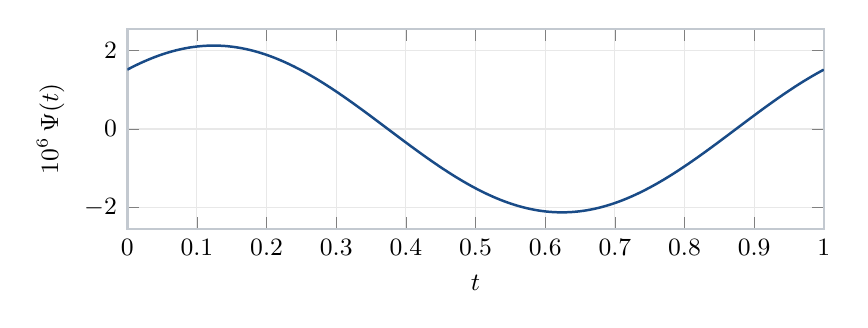
\begin{tikzpicture}
\begin{axis}[
 width=0.86\textwidth,height=0.34\textwidth,
 xmin=0,xmax=1,
 xlabel={$t$},ylabel={$10^{6}\,\Psi(t)$},
 grid=major,major grid style={draw=gray!18},
 axis line style={draw=rulegray},
 tick label style={font=\small},label style={font=\small},
 line width=0.9pt]
\addplot[draw=linkblue,smooth] coordinates {
(0.000000,1.511730) (0.010000,1.602557) (0.020000,1.687060) (0.030000,1.764904)
(0.040000,1.835784) (0.050000,1.899418) (0.060000,1.955556) (0.070000,2.003976)
(0.080000,2.044488) (0.090000,2.076931) (0.100000,2.101177) (0.110000,2.117131)
(0.120000,2.124730) (0.130000,2.123943) (0.140000,2.114774) (0.150000,2.097259)
(0.160000,2.071467) (0.170000,2.037500) (0.180000,1.995492) (0.190000,1.945609)
(0.200000,1.888047) (0.210000,1.823034) (0.220000,1.750826) (0.230000,1.671709)
(0.240000,1.585994) (0.250000,1.494020) (0.260000,1.396150) (0.270000,1.292770)
(0.280000,1.184287) (0.290000,1.071131) (0.300000,0.953748) (0.310000,0.832601)
(0.320000,0.708168) (0.330000,0.580940) (0.340000,0.451419) (0.350000,0.320117)
(0.360000,0.187551) (0.370000,0.054245) (0.380000,-0.079275) (0.390000,-0.212482)
(0.400000,-0.344850) (0.410000,-0.475858) (0.420000,-0.604987) (0.430000,-0.731729)
(0.440000,-0.855584) (0.450000,-0.976061) (0.460000,-1.092687) (0.470000,-1.205000)
(0.480000,-1.312558) (0.490000,-1.414935) (0.500000,-1.511729) (0.510000,-1.602556)
(0.520000,-1.687059) (0.530000,-1.764904) (0.540000,-1.835784) (0.550000,-1.899418)
(0.560000,-1.955557) (0.570000,-2.003977) (0.580000,-2.044489) (0.590000,-2.076933)
(0.600000,-2.101179) (0.610000,-2.117133) (0.620000,-2.124732) (0.630000,-2.123945)
(0.640000,-2.114777) (0.650000,-2.097262) (0.660000,-2.071470) (0.670000,-2.037503)
(0.680000,-1.995495) (0.690000,-1.945611) (0.700000,-1.888049) (0.710000,-1.823036)
(0.720000,-1.750828) (0.730000,-1.671711) (0.740000,-1.585996) (0.750000,-1.494021)
(0.760000,-1.396151) (0.770000,-1.292770) (0.780000,-1.184288) (0.790000,-1.071131)
(0.800000,-0.953748) (0.810000,-0.832600) (0.820000,-0.708167) (0.830000,-0.580938)
(0.840000,-0.451417) (0.850000,-0.320115) (0.860000,-0.187549) (0.870000,-0.054243)
(0.880000,0.079277) (0.890000,0.212484) (0.900000,0.344853) (0.910000,0.475860)
(0.920000,0.604990) (0.930000,0.731732) (0.940000,0.855586) (0.950000,0.976064)
(0.960000,1.092689) (0.970000,1.205002) (0.980000,1.312560) (0.990000,1.414937)
(1.000000,1.511730) 
};
\end{axis}
\end{tikzpicture}
\caption{The periodic correction $\Psi$, magnified by $10^{6}$.  The curve is
indistinguishable from its first Fourier harmonic at this resolution, and the
half-period antisymmetry $\Psi(t+\tfrac12)\approx-\Psi(t)$ visible here is the statement
that the even harmonics are negligible.  The vertical scale is the point of the picture:
the oscillation is a few parts in a million in the logarithm, but it does not tend to
zero.}
\label{fig:Psi-plot}
\end{figure}

\subsection{The finite part at the Mellin origin}

The constant that enters the saddle asymptotic comes from the finite part of
$-\Gamma(z)\zeta(1+z)$ at $z=0$.  Using
\begin{align*}
 \Gamma(z)&=\frac1z-\gamma+
   \left(\frac{\gamma^2}{2}+\frac{\pi^2}{12}\right)z+\bigO(z^2),\\
 \zeta(1+z)&=\frac1z+\gamma-\gamma_1z+\bigO(z^2),
\end{align*}
one finds
\begin{equation}
 -\Gamma(z)\zeta(1+z)+\frac1{z^2}
 =A_0+\bigO(z),                                            \label{eq:A0-finite-part}
\end{equation}
where
\begin{equation}
 A_0=\frac{6\gamma^2+12\gamma_1-\pi^2}{12}.               \label{eq:A0}
\end{equation}
The final constant is
\begin{equation}
 C_F=\frac{A_0}{L}-\frac{7L}{12}-\frac12\log\pi
 \approx-2.02798389863885942397.                           \label{eq:CF}
\end{equation}
The terms $-7L/12$ and $-(1/2)\log\pi$ arise from the dyadic Euler--Maclaurin finite part and
the leading Gaussian saddle mass, respectively.

\section{The corrected sharp asymptotic}
\label{sec:sharp-asymptotic}

\subsection{The lower Lambert coordinate}

For sufficiently small $x>0$, define
\begin{equation}
 W=W_{-1}(-Lx),                                             \label{eq:W-def}
\end{equation}
where $W_{-1}$ is the lower real branch of Lambert's $W$-function \cite{corless1996},
and put
\begin{equation}
 \lambda=\lambda(x)=-\frac{W}{L}.                          \label{eq:lambda-def}
\end{equation}
Then $\lambda\to\infty$ as $x\downarrow0$ and
\begin{equation}
 \lambda2^{-\lambda}=x.                                   \label{eq:lambda-equation}
\end{equation}
Equivalently,
\begin{equation}
 r=2^\lambda=\frac\lambda x.                              \label{eq:saddle-radius}
\end{equation}
The real number $r$ is the explicit Lambert saddle radius used in the contour analysis.

\subsection{The main term}

Define
\begin{equation}
 \mathcal M(x)=
 -\frac L2\lambda^2+
 \left(1+\frac L2\right)\lambda-\frac12\log\lambda
 +C_F+\Psi(\lambda),                                      \label{eq:sharp-main-lambda}
\end{equation}
where $C_F$ is given by \eqref{eq:CF} and $\lambda=\lambda(x)$.  The same expression can be
written compactly in the Lambert variable $W$:
\begin{equation}
 \mathcal M(x)=
 -\frac{7L}{12}-\frac12\log(\pi x)
 +\frac{A_0-W-\tfrac12W^2}{L}
 +\Psi\!\left(-\frac WL\right).                           \label{eq:sharp-main-W}
\end{equation}
The equivalence follows from $W=-L\lambda$ and
$\log x=\log\lambda-L\lambda$.

\begin{theorem}[Corrected sharp endpoint asymptotic]
As $x\downarrow0$,
\begin{equation}
 \boxed{
 \log F(x)=\mathcal M(x)+\bigO\!\left(\frac1{\lambda(x)}\right)
 =\mathcal M(x)+\bigO\!\left(\frac1{-\log x}\right).}     \label{eq:sharp-log-asymptotic}
\end{equation}
Equivalently,
\begin{equation}
 F(x)\sim\exp\mathcal M(x).                               \label{eq:sharp-equivalent}
\end{equation}
\end{theorem}

The periodic term is evaluated at the \emph{exact} phase $\lambda(x)$, not at a truncated
log--log approximation to it.  This matters at the stated error scale.

\subsection{Bromwich inversion}

Because $G(-z)=\E\e^{-zX}$ is entire and $F$ is continuous, Laplace--Stieltjes inversion
gives, for every $r>0$ and $0<x<1$,
\begin{equation}
 F(x)=\frac1{2\pi\ii}\int_{r-\ii\infty}^{r+\ii\infty}
 \frac{\e^{zx}G(-z)}{z}\dd z.                             \label{eq:bromwich}
\end{equation}
Set $z=r(1+\ii\theta)$ and choose $r=2^\lambda=\lambda/x$.  Then
\begin{equation}
 F(x)=\frac{\e^{\lambda+\Lambda(r)}}{2\pi}
 \int_{-\infty}^{\infty}
 \e^{\ii\lambda\theta}
 \frac{G(-r(1+\ii\theta))}{G(-r)}
 \frac{\dd\theta}{1+\ii\theta}.                         \label{eq:bromwich-scaled}
\end{equation}
The exact real decomposition \eqref{eq:Lambda-exact-periodic} at $r=2^\lambda$ gives
\begin{equation}
 \lambda+\Lambda(r)
 =-\frac L2\lambda^2+
 \left(1+\frac L2\right)\lambda+P(\lambda)+E(r).          \label{eq:real-exponent-at-r}
\end{equation}
Since
\begin{equation}
 \overline P=\frac{A_0}{L}-\frac L{12},
 \qquad
 \overline P-\frac12\log(2\pi)=C_F,                      \label{eq:P-mean}
\end{equation}
the missing factors in \eqref{eq:sharp-main-lambda} are exactly the leading Gaussian mass
$1/\sqrt{2\pi\lambda}$ and the centered fluctuation $\Psi=P-\overline P$.

\subsection{The local phase}

Let
\begin{equation}
 u=\log(1+\ii\theta),                                     \label{eq:u-log}
\end{equation}
with the principal logarithm near the saddle.  Subtracting the value at $\theta=0$ from the
complexified version of \eqref{eq:Lambda-exact-periodic}, and including the factor
$(1+\ii\theta)^{-1}$ in \eqref{eq:bromwich-scaled}, gives the local phase
\begin{align}
 \Phi_\lambda(\theta)
 &=\lambda(\ii\theta-u)-\frac u2-\frac{u^2}{2L}
   +\Psi\!\left(\lambda+\frac uL\right)-\Psi(\lambda)
   +\mathcal E_r(\theta),                                 \label{eq:local-phase}
\end{align}
where $\mathcal E_r(0)=0$ and, on a fixed neighborhood of zero, every derivative of
$\mathcal E_r$ is exponentially small in $r$.  This last term comes from the forward tail
$E$ and is far smaller than every power of $1/\lambda$.

The elementary expansion
\begin{equation}
 \log(1+\ii\theta)
 =\ii\theta+\frac{\theta^2}{2}-\frac{\ii\theta^3}{3}
  -\frac{\theta^4}{4}+\bigO(\theta^5)                     \label{eq:log-one-itheta}
\end{equation}
shows that
\begin{equation}
 \lambda(\ii\theta-u)=-\frac{\lambda\theta^2}{2}
 +\frac{\ii\lambda\theta^3}{3}+\frac{\lambda\theta^4}{4}+\
 \bigO(\lambda|\theta|^5).                                \label{eq:gaussian-leading}
\end{equation}
Thus the natural central scale is
\begin{equation}
 \theta=\frac v{\sqrt\lambda}.                            \label{eq:central-scale}
\end{equation}
Uniformly for $|v|$ growing sufficiently slowly with $\lambda$,
\begin{equation}
 \Phi_\lambda(v/\sqrt\lambda)
 =-\frac{v^2}{2}+\lambda^{-1/2}P_1(v;\lambda)
 +\lambda^{-1}P_2(v;\lambda)
 +\bigO\!\left(\lambda^{-3/2}(1+|v|^9)\right),            \label{eq:phase-first-expansion}
\end{equation}
where
\begin{align}
 A(u)&=\frac{\Psi'(u)}L-\frac12,                           \label{eq:A-periodic}\\
 B(u)&=-\frac14+\frac1{2L}+\frac{\Psi'(u)}{2L}
       -\frac{\Psi''(u)}{2L^2},                           \label{eq:B-periodic}\\
 P_1(v;u)&=\ii\left(A(u)v+\frac{v^3}{3}\right),           \label{eq:P1}\\
 P_2(v;u)&=\frac{v^4}{4}+B(u)v^2.                         \label{eq:P2}
\end{align}
In \eqref{eq:phase-first-expansion}, the second argument is $u=\lambda$.

\subsection{Central and tail estimates}

For completeness, the quantitative saddle proof is organized by the following estimates.
They are stated here in the form needed for the argument; the formal development proves them
with explicit domains and constants.

\begin{lemma}[Central expansion]
For every fixed truncation order $N$, there is $\delta>0$ such that on
$|\theta|\le\delta$ the exponent in \eqref{eq:bromwich-scaled} admits a Taylor expansion
through order $N$ after the scaling \eqref{eq:central-scale}.  Its coefficients are smooth
$1$-periodic functions of $\lambda$, and the remainder is dominated by a polynomial in $v$
times the next power of $\lambda^{-1/2}$.
\end{lemma}

\begin{proof}
The logarithm in \eqref{eq:u-log} is analytic for $|\theta|<1$.  The periodic function
$\Psi$ is smooth with bounded derivatives of every order.  Taylor's theorem applied to each
term of \eqref{eq:local-phase}, together with the exponentially small bounds on
$\mathcal E_r$, gives a uniform expansion.  The dependence on $\lambda$ occurs only through
$\Psi^{(j)}(\lambda)$, hence is periodic.
\end{proof}

\begin{lemma}[Gaussian domination]
There are positive constants $c,\delta$ and $\lambda_0$ such that, for
$\lambda\ge\lambda_0$ and $|\theta|\le\delta$,
\begin{equation}
 \Re\Phi_\lambda(\theta)\le-c\lambda\theta^2.             \label{eq:central-domination}
\end{equation}
\end{lemma}

\begin{proofidea}
The exact function $\Re(\ii\theta-\log(1+\ii\theta))
=-(1/2)\log(1+\theta^2)$ supplies the negative quadratic term.  All remaining terms in
\eqref{eq:local-phase} have bounded first and second derivatives on a fixed neighborhood.
For large $\lambda$ the $-\lambda\theta^2/2$ contribution dominates them.
\end{proofidea}

\begin{lemma}[Off-saddle decay]
For each $N$ one may choose the central window so that the contribution to
\eqref{eq:bromwich-scaled} outside that window is $O(\lambda^{-N})$ relative to the leading
saddle mass.
\end{lemma}

\begin{proofidea}
Split the negative-Laplace product at the dyadic index nearest $\lambda$.  In the intermediate
range, a positive proportion of the factors have arguments of order one and their moduli are
strictly smaller off the real axis, yielding exponential decay in $\lambda\theta^2$.  In the
far range, repeated use of the sinc/Laplace product bounds gives arbitrarily high polynomial
decay.  The two bounds overlap and cover the whole complement of the central window.  The
factor $(1+\ii\theta)^{-1}$ is harmless.
\end{proofidea}

These lemmas justify extending the scaled central integral to the entire real $v$-axis and
integrating its expansion term by term against $\e^{-v^2/2}$.

\subsection{Completion of the leading proof}

Keeping only the Gaussian term in \eqref{eq:phase-first-expansion} gives
\begin{equation}
 \int_\R\e^{\Phi_\lambda(\theta)}\dd\theta
 =\frac1{\sqrt\lambda}\int_\R\e^{-v^2/2}\dd v
  \left(1+\bigO(\lambda^{-1})\right)
 =\sqrt{\frac{2\pi}{\lambda}}
  \left(1+\bigO(\lambda^{-1})\right).                     \label{eq:leading-saddle-mass}
\end{equation}
The term of order $\lambda^{-1/2}$ integrates to zero because $P_1$ is odd in $v$ and purely
imaginary.  Combining \eqref{eq:real-exponent-at-r}, \eqref{eq:P-mean}, and
\eqref{eq:leading-saddle-mass} yields
\begin{equation*}
 \log F(x)
 =-\frac L2\lambda^2+
 \left(1+\frac L2\right)\lambda-\frac12\log\lambda
 +C_F+\Psi(\lambda)+\bigO(\lambda^{-1}),
\end{equation*}
which is \eqref{eq:sharp-log-asymptotic}.  Finally,
$\lambda\asymp-\log x$ follows from \eqref{eq:lambda-equation}, so the two displayed error
scales are equivalent.

\section{First correction and the all-orders saddle expansion}
\label{sec:full-asymptotic}

The leading theorem leaves an error of order $1/\lambda$.  The same contour analysis can be
continued to arbitrary order.  The coefficient functions are periodic because every local
coefficient is built from derivatives of $\Psi$ evaluated at the exact phase $\lambda$.

\subsection{The first correction}

Expand the exponential in \eqref{eq:phase-first-expansion}:
\begin{align}
 \e^{\Phi_\lambda(v/\sqrt\lambda)}
 &=\e^{-v^2/2}\Bigl[1+\lambda^{-1/2}P_1(v;\lambda) \\[-0.3ex]
 &\qquad+\lambda^{-1}\bigl(P_2(v;\lambda)+\tfrac12P_1(v;\lambda)^2\bigr)
 +\bigO(\lambda^{-3/2}(1+|v|^{12}))\Bigr].                \label{eq:exp-phase-first}
\end{align}
Let $Z$ be a standard normal random variable.  Since
\begin{equation}
 \E Z^2=1,\qquad \E Z^4=3,\qquad \E Z^6=15,               \label{eq:gaussian-moments}
\end{equation}
the normalized coefficient of $\lambda^{-1}$ in the saddle mass is
\begin{align}
 b_1(u)
 &=\E\left[P_2(Z;u)+\tfrac12P_1(Z;u)^2\right]             \notag\\
 &=\frac34+B(u)-\frac12\left(A(u)^2+2A(u)+\frac53\right). \label{eq:b1-gaussian}
\end{align}
Substituting \eqref{eq:A-periodic} and \eqref{eq:B-periodic} simplifies the expression
considerably.

\begin{theorem}[First saddle correction]
Define
\begin{equation}
 A_1(u)=\frac1{24}+\frac1{2L}
 -\frac{\Psi''(u)+\Psi'(u)^2}{2L^2}.                       \label{eq:A1}
\end{equation}
Then
\begin{equation}
 \boxed{
 \log F(x)=\mathcal M(x)+\frac{A_1(\lambda(x))}{\lambda(x)}
 +\bigO\!\left(\lambda(x)^{-2}\right).}                  \label{eq:first-corrected-asymptotic}
\end{equation}
\end{theorem}

\begin{proof}
The order-$\lambda^{-1/2}$ term in \eqref{eq:exp-phase-first} is odd and integrates to zero.
Equation \eqref{eq:b1-gaussian} gives the first nonzero relative correction to the integral.
A direct simplification yields \eqref{eq:A1}.  If the normalized saddle mass is
$1+b_1/\lambda+O(\lambda^{-2})$, then its logarithm is
$b_1/\lambda+O(\lambda^{-2})$, so the same coefficient appears in the logarithmic expansion.
The off-saddle contribution is smaller than the stated remainder by the tail estimates of the
preceding section.
\end{proof}

The constant part $1/24+1/(2L)$ is the usual type of Gaussian/curvature correction.  The
terms involving $\Psi'$ and $\Psi''$ record the fact that the log-periodic environment is not
constant across the saddle width.

\subsection{All orders}

At order $N$, Taylor expansion of \eqref{eq:local-phase} produces finitely many polynomials
in $v$ whose coefficients are differential polynomials in
\begin{equation*}
 \Psi'(u),\Psi''(u),\ldots,\Psi^{(2N)}(u).
\end{equation*}
After exponentiation, all odd powers of $\lambda^{-1/2}$ integrate to zero by parity.  The
remaining Gaussian moments are integers, so one obtains integer powers of $1/\lambda$.

\begin{theorem}[Full logarithmic expansion]
There are smooth $1$-periodic functions $A_j:\R\to\R$, $j\ge0$, with
$A_0=0$ and $A_1$ given by \eqref{eq:A1}, such that for every $N\ge1$,
\begin{equation}
 \boxed{
 \log F(x)=\mathcal M(x)+
   \sum_{j=1}^{N-1}\frac{A_j(\lambda(x))}{\lambda(x)^j}
   +\bigO\!\left(\lambda(x)^{-N}\right)}                 \label{eq:all-orders-log}
\end{equation}
as $x\downarrow0$.
\end{theorem}

\begin{proofidea}
Fix $N$.  Expand the analytic local phase through sufficiently high order in
$\lambda^{-1/2}$, with a Gaussian-dominated remainder.  Exponentiate using complete Bell
polynomials, integrate term by term, and discard odd terms.  The quantitative tail theorem
makes the complement of the central region $O(\lambda^{-N})$.  This gives a relative saddle
mass expansion
\begin{equation}
 1+\sum_{j=1}^{N-1}\frac{b_j(\lambda)}{\lambda^j}
 +O(\lambda^{-N}),                                        \label{eq:relative-mass-series}
\end{equation}
where every $b_j$ is smooth and periodic.  Taking the formal logarithm defines the $A_j$.
If
\begin{equation*}
 \log\left(1+\sum_{j\ge1}b_jz^j\right)=\sum_{j\ge1}A_jz^j,
\end{equation*}
then the coefficients may be generated recursively by
\begin{equation}
 A_n=b_n-\frac1n\sum_{k=1}^{n-1}kA_kb_{n-k}.               \label{eq:log-coefficient-recurrence}
\end{equation}
All operations preserve smooth periodic dependence on the phase.
\end{proofidea}

This form of the expansion is preferable to a very long series in nested logarithms.  The
exact Lambert coordinate absorbs the dominant implicit inversion, while the exact periodic
phase prevents phase errors from being magnified into false remainder claims.

\section{Elementary log--log forms and the missing periodic term}
\label{sec:elementary-asymptotic}

Lambert $W$ gives the cleanest formula, but an expansion in elementary logarithms is useful
for comparison with published displays.  It must, however, retain $\Psi$ at the exact Lambert
phase.

\subsection{The literal small-$x$ expansion}

Put
\begin{equation}
 S=-\log x,\qquad m=\log S,\qquad a=\log L.                \label{eq:S-m-a}
\end{equation}
Thus $S\to\infty$ as $x\downarrow0$.  Define the nonperiodic elementary expression
\begin{align}
 \mathcal E_0(x)
={}&-\frac{S^2}{2L}-\frac{Sm}{L}
 +\left(\frac12+\frac{1+a}{L}\right)S                     \notag\\
 &-\frac{m^2}{2L}+\frac{am}{L}
 +\frac{6\gamma^2+12\gamma_1-\pi^2-6a^2}{12L}
 -\frac{7L}{12}-\frac12\log\pi                           \notag\\
 &-\frac{m^2}{2LS}+\frac{am}{LS}.                         \label{eq:elementary-main}
\end{align}

\begin{theorem}[Corrected elementary expansion]
As $x\downarrow0$,
\begin{equation}
 \boxed{
 \log F(x)=\mathcal E_0(x)+\Psi(\lambda(x))
 +\bigO\!\left(\frac1{-\log x}\right).}                  \label{eq:corrected-elementary}
\end{equation}
\end{theorem}

\begin{proofidea}
The standard lower-branch Lambert expansion solves
$\lambda L-\log\lambda=S$ by successive substitution.  Substituting that expansion into
\eqref{eq:sharp-main-lambda}, and retaining enough phase terms to control the amplified
quadratic contribution, gives \eqref{eq:elementary-main}.  A coarse two-term approximation to
$\lambda$ is insufficient: because the main exponent contains $-L\lambda^2/2$, an error
$\delta\lambda$ contributes about $-L\lambda\delta\lambda$, so the phase must be known one
order more accurately than a naive count suggests.  The fourth Lambert phase term in the
formal proof is exactly what reduces the residual to $O(1/S)$.
\end{proofidea}

In the original variable $\ell=\log x<0$, the same expression is
\begin{align}
 \mathcal E_0(x)
={}&-\frac{\ell^2}{2L}+\frac{\ell\log(-\ell)}L
 -\left(\frac12+\frac{1+\log L}{L}\right)\ell             \notag\\
 &-\frac{\log^2(-\ell)}{2L}
 +\frac{\log L\,\log(-\ell)}L                             \notag\\
 &+\frac{6\gamma^2+12\gamma_1-\pi^2-6\log^2L}{12L}
 -\frac{7L}{12}-\frac12\log\pi                           \notag\\
 &+\frac{\log^2(-\ell)}{2L\ell}
 -\frac{\log L\,\log(-\ell)}{L\ell}.                   \label{eq:elementary-main-ell}
\end{align}
This is the literal elementary display formalized in the repository, with the periodic term
added separately.

\subsection{The dyadic logarithmic scale}

Set $x=2^{-t}$ and let
\begin{equation}
 \lambda_t=-\frac1L W_{-1}(-L2^{-t}).                      \label{eq:lambda-t}
\end{equation}
Then $\lambda_t$ is the unique large solution of
\begin{equation}
 \lambda_t-\log_2\lambda_t=t.                             \label{eq:lambda-t-fixed}
\end{equation}
Its first terms are
\begin{equation}
 \lambda_t=t+\frac{\log t}{L}
 +\frac{\log t}{L^2t}
 +\frac{\log t-\tfrac12\log^2t}{L^3t^2}
 +\bigO\!\left(\frac{\log^3t}{t^3}\right).              \label{eq:lambda-t-expansion}
\end{equation}
Define
\begin{align}
 \mathcal D_0(t)
={}&-\frac L2t^2-t\log t+
 \left(1+\frac L2\right)t-\frac{\log^2t}{2L}+C_F
 -\frac{\log^2t}{2L^2t}.                                 \label{eq:dyadic-main}
\end{align}

\begin{theorem}[Corrected dyadic-scale expansion]
As $t\to\infty$,
\begin{equation}
 \boxed{
 \log F(2^{-t})=\mathcal D_0(t)+\Psi(\lambda_t)
 +\bigO(t^{-1}).}                                         \label{eq:dyadic-asymptotic}
\end{equation}
\end{theorem}

The literal substitution of $x=2^{-t}$ into \eqref{eq:elementary-main} differs from
$\mathcal D_0(t)$ by the explicit term
\begin{equation}
 \frac{\log^2L}{2L^2t},                                   \label{eq:literal-dyadic-difference}
\end{equation}
which is itself $O(1/t)$.  Thus both nonperiodic displays are valid at the stated precision,
but they are not algebraically identical.

\subsection{Why the uncorrected formula is false at the claimed scale}

Let $\mathcal M_0(x)=\mathcal M(x)-\Psi(\lambda(x))$ be the nonperiodic Lambert main.  From
\eqref{eq:sharp-log-asymptotic},
\begin{equation}
 \log F(x)-\mathcal M_0(x)=\Psi(\lambda(x))+O(1/\lambda(x)). \label{eq:uncorrected-residual}
\end{equation}
Since $\Psi$ is nonconstant, the right side does not tend to zero.

\begin{proposition}[Failure without the periodic correction]
The relation
\begin{equation}
 \log F(x)=\mathcal M_0(x)+O(1/(-\log x))                  \label{eq:false-uncorrected}
\end{equation}
 is false.  In fact $F(x)/\exp(\mathcal M_0(x))$ has distinct subsequential limits.
\end{proposition}

\begin{proof}
Choose $u,v\in[0,1)$ with $\Psi(u)\ne\Psi(v)$.  Set
\begin{equation*}
 \lambda_n=n+u,
 \qquad x_n=\lambda_n2^{-\lambda_n}.
\end{equation*}
Then $x_n\downarrow0$ and the exact Lambert phase of $x_n$ is $\lambda_n$.  Hence
\begin{equation*}
 \log F(x_n)-\mathcal M_0(x_n)\longrightarrow\Psi(u).
\end{equation*}
The analogous sequence with phase $n+v$ tends to $\Psi(v)$.  Since
$1/(-\log x)\to0$, the bound \eqref{eq:false-uncorrected} is impossible.  Exponentiating
gives distinct ratio limits $\e^{\Psi(u)}$ and $\e^{\Psi(v)}$.
\end{proof}

Numerically the discrepancy is minute because the first Fourier mode has size about
$10^{-6}$, but asymptotic equivalence is a limit statement, not a graphical tolerance.  A
nonzero bounded oscillation cannot be hidden inside an error term that tends to zero.

\subsection{Symmetry at the right endpoint}

The symmetry $F(1-x)=1-F(x)$ immediately transfers the left-endpoint expansion to the right:
\begin{equation}
 1-F(1-x)=F(x).                                            \label{eq:right-endpoint-sym}
\end{equation}
Thus the same Lambert phase, periodic fluctuation, and all-orders coefficients describe the
survival probability near $1$.

\section{Consequences of the endpoint expansion}
\label{sec:asymptotic-consequences}

The full sharp formula immediately settles several qualitative questions that are otherwise
awkward to read from the differential equation.

\begin{theorem}[Quadratic logarithmic law]
As $x\downarrow0$,
\begin{equation}
 \frac{\log F(x)}{(\log x)^2}\longrightarrow-\frac1{2\log2}. \label{eq:quadratic-log-law}
\end{equation}
Equivalently, on the dyadic scale,
\begin{equation}
 \log F(2^{-t})\sim-\frac{\log2}{2}t^2.                    \label{eq:dyadic-quadratic-law}
\end{equation}
\end{theorem}

\begin{proof}
In \eqref{eq:sharp-main-lambda}, $\lambda\sim S/L$ with $S=-\log x$.  The quadratic term
$-L\lambda^2/2$ dominates the linear term, the logarithmic term, and the bounded periodic
correction.  Substitution gives \eqref{eq:quadratic-log-law}.
\end{proof}

\begin{corollary}[Between powers and pure endpoint exponentials]
\label{cor:decay-comparison}
For every $N>0$ and every $c>0$,
\begin{equation}
 F(x)=o(x^N),                                               \label{eq:faster-than-powers}
\end{equation}
and
\begin{equation}
 \e^{-c/x}=o(F(x))                                         \label{eq:slower-than-exp-inv-x}
\end{equation}
as $x\downarrow0$.
\end{corollary}

\begin{proof}
The logarithm of $x^N$ is $-NS$, whereas
$\log F(x)\sim-S^2/(2L)$, so $F(x)/x^N\to0$.  On the other hand,
$\log\e^{-c/x}=-c\e^S$, which is much more negative than $-S^2/(2L)$; therefore
$\e^{-c/x}/F(x)\to0$.
\end{proof}

This places the endpoint decay in an intermediate regime.  The function is flatter than any
finite algebraic order, as every compactly supported smooth function must be at its support
boundary, but it is vastly larger than the familiar model $\e^{-1/x}$.

\begin{corollary}[Asymptotics of reciprocal-power values]
For integers $n\to\infty$,
\begin{align}
 \log F(2^{-n})
={}&-\frac L2n^2-n\log n+
 \left(1+\frac L2\right)n-\frac{\log^2n}{2L}+C_F           \notag\\
 &-\frac{\log^2n}{2L^2n}+\Psi(\lambda_n)+O(n^{-1}),       \label{eq:integer-dyadic-asymptotic}
\end{align}
where $\lambda_n$ is defined by \eqref{eq:lambda-t}.  Combining this with
\eqref{eq:F-inverse-power} gives an equally sharp expansion for the half moments $d_n$.
\end{corollary}

The formula shows why a fixed multiplicative constant cannot complete a recurrence-based
ansatz for $F(2^{-n})$: the fractional parts of $\lambda_n$ drift, and the factor
$\exp\Psi(\lambda_n)$ is nonconstant.

\section{The Fourier--Legendre expansion of $\Up$}
\label{sec:legendre}

A second exact spectral representation uses the ordinary Legendre polynomials $P_n$ on
$[-1,1]$.  Unlike the Fourier transform, this is a polynomial expansion on the natural
support interval, and its coefficients can be expressed by the reciprocal-power dyadic
values already computed.

\subsection{Orthogonality and coefficients}

Normalize the Legendre polynomials by $P_n(1)=1$.  They satisfy
\begin{equation}
 -\frac{\dd}{\dd x}\left((1-x^2)P_n'(x)\right)
 =n(n+1)P_n(x),                                            \label{eq:legendre-ode}
\end{equation}
with orthogonality
\begin{equation}
 \int_{-1}^{1}P_m(x)P_n(x)\dd x
 =\frac{2}{2n+1}\,\delta_{mn}.                            \label{eq:legendre-orthogonality}
\end{equation}
For a continuous function $f$, define
\begin{equation}
 \alpha_n(f)=\frac{2n+1}{2}\int_{-1}^{1}f(x)P_n(x)\dd x. \label{eq:legendre-coefficient}
\end{equation}
Because $\Up$ is even and $P_n(-x)=(-1)^nP_n(x)$,
\begin{equation}
 \alpha_{2n+1}(\Up)=0.                                    \label{eq:odd-legendre-zero}
\end{equation}
Put
\begin{equation}
 u_n=\alpha_{2n}(\Up)
 =\frac{4n+1}{2}\int_{-1}^{1}\Up(x)P_{2n}(x)\dd x.        \label{eq:un-legendre}
\end{equation}

\subsection{Exact coefficient formula}

The even Legendre polynomial has the finite power expansion
\begin{equation}
 P_{2n}(x)=4^{-n}\sum_{k=0}^{n}(-1)^{n+k}
 \binom{2n}{n+k}\binom{2n+2k}{2n}x^{2k}.                  \label{eq:even-legendre-power}
\end{equation}
The moment-to-dyadic bridge is
\begin{equation}
 c_k=2(2k)!\,2^{\binom{2k+1}{2}}F(2^{-2k-1}).              \label{eq:ck-dyadic-bridge}
\end{equation}
This is \eqref{eq:moment-endpoint-bridge} with an even exponent, together with symmetry.

\begin{theorem}[Exact Legendre coefficients]
For every $n\ge0$,
\begin{align}
 u_n
={}&4^{-n}(4n+1)\sum_{k=0}^{n}(-1)^{n+k}
 \binom{2n}{n+k}\binom{2n+2k}{2n}                         \notag\\
 &\hspace{5em}\times(2k)!\,2^{\binom{2k+1}{2}}
 F(2^{-2k-1}).                                             \label{eq:legendre-exact-coeff}
\end{align}
In particular every $u_n$ is rational.
\end{theorem}

\begin{proof}
Insert \eqref{eq:even-legendre-power} into \eqref{eq:un-legendre} and interchange the finite
sum with the integral.  The integral of $x^{2k}\Up(x)$ is $c_k$.  Substitution of
\eqref{eq:ck-dyadic-bridge} cancels the factor $1/2$ in
\eqref{eq:un-legendre} and gives \eqref{eq:legendre-exact-coeff}.
\end{proof}

Thus the entire polynomial spectral expansion is anchored in the same exact arithmetic table
$F(2^{-m})$ that drives the bit-recursive evaluator.

\begin{example}[The first two Legendre coefficients]        \label{ex:mom-legendre-first}
Take $n=0$ and $n=1$ in \eqref{eq:un-legendre}.  Since $P_0=1$ and
$P_2(x)=(3x^2-1)/2$,
\begin{align*}
 u_0&=\frac12\int_{-1}^{1}\Up(x)\dd x=\frac{c_0}{2}=\frac12,\\
 u_1&=\frac52\int_{-1}^{1}\Up(x)\frac{3x^2-1}{2}\dd x
 =\frac54\bigl(3c_1-c_0\bigr)=\frac54\left(\frac13-1\right)=-\frac56 .
\end{align*}
The exact formula \eqref{eq:legendre-exact-coeff} returns the same two numbers without
reference to the moments.  For $n=0$ the sum has the single term
$\binom00\binom00\,0!\,2^{\binom12}F(2^{-1})=\tfrac12$, so $u_0=\tfrac12$.  For $n=1$,
\begin{equation*}
 u_1=\frac54\left[-\binom21\binom22\,0!\,2^{\binom12}F(2^{-1})
 +\binom22\binom42\,2!\,2^{\binom32}F(2^{-3})\right]
 =\frac54\left[-1+\frac{96}{288}\right]=-\frac56,
\end{equation*}
using $\binom12=0$, $\binom32=3$, $F(2^{-1})=\tfrac12$ and $F(2^{-3})=\tfrac1{288}$ from
\eqref{eq:F-inverse-table}.  Hence the Fourier--Legendre expansion \eqref{eq:legendre-series}
begins
\begin{equation}
 \Up(t)=\frac12-\frac56P_2(t)+\cdots.                       \label{eq:mom-legendre-first-terms}
\end{equation}
Both values are stated in the normalization \eqref{eq:un-legendre} used here, in which
$u_n=\alpha_{2n}(\Up)$ already carries the factor $(4n+1)/2$ of
\eqref{eq:legendre-coefficient}; the bare integrals are
$\int_{-1}^{1}\Up P_0=1$ and $\int_{-1}^{1}\Up P_2=-\tfrac13$.  The negative sign of $u_1$ is
genuine and reflects the fact that $\Up$ is more sharply peaked at the origin than the
constant $\tfrac12$.
\end{example}

\subsection{Absolute and uniform convergence}

The Legendre Sturm--Liouville operator
\begin{equation}
 \mathcal Lf=-\frac{\dd}{\dd x}\left((1-x^2)f'(x)\right)   \label{eq:SL-operator}
\end{equation}
is formally self-adjoint on $[-1,1]$.  Boundary terms vanish because of the factor
$1-x^2$.  Repeated integration by parts therefore gives, for $n\ge1$,
\begin{equation}
 \alpha_n(f)=\frac{2n+1}{2[n(n+1)]^m}
 \int_{-1}^{1}(\mathcal L^mf)(x)P_n(x)\dd x.              \label{eq:legendre-decay-ibp}
\end{equation}
Since $|P_n(x)|\le1$ on $[-1,1]$, any $C^\infty$ function has coefficients that decay faster
than every power of $n$.

\begin{theorem}[Uniform Legendre series]
On the entire closed interval $[-1,1]$,
\begin{equation}
 \boxed{
 \Up(x)=\sum_{n=0}^{\infty}u_nP_{2n}(x).}                 \label{eq:legendre-series}
\end{equation}
The series converges absolutely and uniformly, including at both endpoints.
\end{theorem}

\begin{proof}
Apply \eqref{eq:legendre-decay-ibp} to $f=\Up$.  Choosing $m\ge2$ gives
$|\alpha_n(\Up)|\le Cn^{-3}$, say.  Since $|P_n|\le1$, the Weierstrass test gives absolute
and uniform convergence.  Let the uniform sum be $g$.  Orthogonality shows that $g$ and
$\Up$ have the same Legendre coefficients.  Completeness of the Legendre polynomials in
$L^2[-1,1]$ implies $g=\Up$ almost everywhere, and continuity upgrades equality to every
point.  Odd coefficients vanish by \eqref{eq:odd-legendre-zero}, leaving
\eqref{eq:legendre-series}.
\end{proof}

The endpoint statement is worth emphasizing.  Generic Fourier--Legendre convergence theorems
are often quoted only on the open interval, or with an endpoint average.  Here smoothness and
absolute uniform convergence give the literal values $\Up(\pm1)=0$.

\subsection{A practical polynomial approximation}

Truncating \eqref{eq:legendre-series} at $n=N$ gives a polynomial of degree $2N$ with exact
rational coefficients after expanding the $P_{2n}$.  The error is bounded by
\begin{equation}
 \left\|\Up-\sum_{n=0}^{N}u_nP_{2n}\right\|_\infty
 \le\sum_{n>N}|u_n|.                                      \label{eq:legendre-tail-bound}
\end{equation}
Repeated use of \eqref{eq:legendre-decay-ibp} supplies arbitrarily high algebraic tail bounds.
For moderate precision this method is attractive: all coefficients are exact, evaluation is
stable on $[-1,1]$, and the approximation respects evenness automatically.


\subsection{Least-squares optimality of the partial sums}

The Legendre truncation is not only a convenient polynomial approximation; it is the exact
orthogonal projection in $L^2[-1,1]$.  Define
\begin{equation}
 S_N(x)=\sum_{n=0}^{N}u_nP_{2n}(x).                       \label{eq:legendre-partial-sum}
\end{equation}

\begin{theorem}[Pythagorean error identity]
For every real polynomial $p$ of degree at most $2N+1$,
\begin{equation}
 \int_{-1}^{1}\bigl(\Up(x)-p(x)\bigr)^2\dd x
 =
 \int_{-1}^{1}\bigl(\Up(x)-S_N(x)\bigr)^2\dd x
 +
 \int_{-1}^{1}\bigl(p(x)-S_N(x)\bigr)^2\dd x.             \label{eq:legendre-pythagorean}
\end{equation}
Consequently $S_N$ is the unique least-squares approximant among all such polynomials.
\end{theorem}

\begin{proof}
Every polynomial of degree at most $2N+1$ is a linear combination of
$P_0,\ldots,P_{2N+1}$.  By construction, $\Up-S_N$ is orthogonal to each even basis
element through $P_{2N}$; by evenness it is also orthogonal to every odd basis element.
Hence
\begin{equation*}
 \int_{-1}^{1}(\Up-S_N)(p-S_N)=0.
\end{equation*}
Expanding
$\Up-p=(\Up-S_N)-(p-S_N)$ gives \eqref{eq:legendre-pythagorean}.  Equality with the
minimum forces the final nonnegative integral to vanish.  A polynomial vanishing almost
everywhere vanishes identically, so $p=S_N$.
\end{proof}

The one-degree slack is genuine: the odd coefficient of $P_{2N+1}$ is zero.  Thus a partial
sum visibly of degree $2N$ is already optimal in the larger space of degree at most
$2N+1$.


\section{Additional summation and spectral identities}
\label{sec:additional-identities}

\subsection{The cosine series on the support}

Periodize $\Up$ with period $2$.  Since neighboring support intervals meet only at zeros, the
periodization agrees with $\Up$ on $[-1,1]$.  Its Fourier coefficients are
$\widehat{\Up}(n/2)/2$, so rapid Fourier decay gives the uniformly convergent cosine series
\begin{equation}
 \Up(x)=\frac12+
 \sum_{n=1}^{\infty}\widehat{\Up}(n/2)\cos(\pi nx),
 \qquad -1\le x\le1.                                     \label{eq:up-cosine-series}
\end{equation}
Using \eqref{eq:sinc-product}, every coefficient is an explicit infinite product.  Many
coefficients vanish because one of the sinc factors is evaluated at a nonzero integer.

\subsection{Scaled partitions}

Equation \eqref{eq:partition-unity} may be differentiated term by term.  For $j\ge1$,
\begin{equation}
 \sum_{k\in\Z}\Up^{(j)}\!\left(t+\frac{k}{m}\right)=0.    \label{eq:derivative-partition}
\end{equation}
The sums are locally finite.  Combining this with \eqref{eq:up-derivatives} turns the
identity into exact finite cancellations among signed translates of $\mathcal F$ at dyadic
scales.

\subsection{Mean and variance of the Fabius law}

From the random-series representation,
\begin{equation}
 \E X=\sum_{n\ge0}\frac{1/2}{2^{n+1}}=\frac12.             \label{eq:X-mean}
\end{equation}
Since $\Var(U_n)=1/12$ and the coordinates are independent,
\begin{equation}
 \Var(X)=\frac1{12}\sum_{n\ge0}4^{-n-1}=\frac1{36}.        \label{eq:X-variance}
\end{equation}
For $Y=2X-1$, this gives $\E Y=0$ and $\Var(Y)=1/9$, agreeing with $c_1=1/9$.
Higher even moments are exactly the $c_n$ of \eqref{eq:c-recurrence}.

\subsection{An exact self-convolution law}

Splitting the random series into its even and odd coordinates gives two independent scaled
copies with different weights.  At the transform level this is the factorization
\begin{equation}
 \widehat{\Up}(z)
 =\widehat{\Up}(z/2)\sinc(\pi z).                          \label{eq:transform-self-convolution}
\end{equation}
In physical space,
\begin{equation}
 \Up(x)=2\int_{-1/2}^{1/2}\Up(2x-2t)\dd t
       =\int_{2x-1}^{2x+1}\Up(y)\dd y,                  \label{eq:up-convolution-refinement}
\end{equation}
with the normalization understood as convolution with the uniform density on
$[-1/2,1/2]$.  Differentiating this integral refinement recovers
\eqref{eq:up-diffeq}.  Conversely, integrating the differential equation and using compact
support recovers the convolution law.

\section{Computation in exact and numerical regimes}
\label{sec:computation}

The identities above do not lead to a single universally best numerical method.  They lead to
a collection of algorithms adapted to different questions.  This section makes the
distinctions explicit, since confusing an exact arithmetic formula with an endpoint
asymptotic is as unhelpful as using a dense dyadic table to evaluate one value at
$2^{-10^6}$.

\subsection{Which representation should be used?}

\begin{center}
\begin{tabularx}{0.96\textwidth}{@{}p{0.20\textwidth}X X@{}}
\toprule
Representation & Principal strength & Principal limitation\\
\midrule
Contraction fixed point &
A direct constructive proof; after $m$ iterations the uniform error is geometrically small. &
Produces approximating functions rather than exact individual values.\\
Finite convolution / probability &
Positive approximants, natural sampling, and a transparent explanation of smoothness. &
High resolution requires many convolution levels.\\
Centered finite spline &
An explicit finite formula with certified uniform error at most $2^{-p}$. &
Direct summation has exponentially many terms unless its recursion is compiled.\\
Fourier sinc product &
Entire transform, rapid frequency decay, and efficient evaluation away from extreme
endpoint cancellation. &
Recovering a tiny value of $F(x)$ by oscillatory inversion may lose many digits.\\
Exact dyadic formula &
A closed rational answer and an algebraic proof of representation invariance. &
The literal Thue--Morse sum may contain exponentially many terms.\\
Bit-recursive Taylor evaluator &
Exact rational arithmetic with at most one recursive call per set bit of the numerator. &
Rational numerators and denominators themselves become very large.\\
Legendre series &
Uniform polynomial approximation on the full closed support, with exact coefficients. &
Not specially adapted to resolving the boundary layer at a tiny $x$.\\
Lambert saddle expansion &
Stable evaluation of $\log F(x)$ at extraordinarily small positive $x$. &
Asymptotic rather than exact; the periodic correction must be retained.\\
\bottomrule
\end{tabularx}
\end{center}

For the fixed-point construction, let $T$ be the transform of
\eqref{eq:fixed-transform}.  If $f_0$ is any admissible continuous function, then
\begin{equation}
 \|T^m f_0-F\|_\infty
 \le 2^{-m}\|f_0-F\|_\infty
 \le 2^{-m}.                                               \label{eq:fixed-point-error}
\end{equation}
Thus the contraction proof itself is a certified numerical scheme.  It is excellent for
coarse graphs and for constructing a first approximation without any prior arithmetic
tables.  Exact dyadic computation, however, should use the rational recurrences.

\subsection{Precomputing the reciprocal-power table}

Put
\begin{equation}
 V_n=F(2^{-n}).
\end{equation}
Eliminating $d_n$ from \eqref{eq:d-recurrence} and
\eqref{eq:F-inverse-power} gives an especially convenient recurrence involving only earlier
$V_k$:
\begin{equation}
 V_0=1,\qquad
 V_{n+1}
 =
 \frac{1}{2^{n+1}-1}
 \sum_{k=0}^{n}
 \frac{V_k}
 {2^{\binom{n+1}{2}-\binom{k}{2}}(n+2-k)!}.               \label{eq:V-table-recurrence}
\end{equation}
Every operation is rational.  A practical implementation stores the values in an array,
reduces each rational after every addition, and reuses factorials and powers of two.  This
table is precisely the data required by the Taylor blocks in
\eqref{eq:taylor-block}.

There are three useful normalization choices.

\begin{enumerate}
\item Store $V_n$ directly.  This makes the public API simple and is ideal when values are
      eventually returned as rational numbers.
\item Store $d_n=n!2^{\binom n2}V_n$.  The recurrence has smaller explicit powers of two,
      and the parity theorem provides a strong integrity check.
\item Store the division-free natural numerators $D_n$ of the half moments, defined by
      \eqref{eq:d-normalized}.  This avoids
      fraction reduction inside the recurrence but requires restoring a known structured
      denominator at the end.
\end{enumerate}

The third choice is usually best for bulk generation; the first is usually best for a small
library interface.

\subsection{Operation count of the bit recursion}

Suppose $0<a<2^n$, and write the set-bit positions of $a$ in decreasing order as
\begin{equation}
 b_1>b_2>\cdots>b_h\ge0,\qquad
 a=\sum_{j=1}^{h}2^{b_j}.                                 \label{eq:set-bit-positions}
\end{equation}
The evaluator of \cref{alg:dyadic-evaluator} makes exactly $h=\operatorname{popcount}(a)$
nontrivial recursive calls.  At the $j$th call, the Taylor order is $n-b_j$.  Hence the
number of rational multiply-add steps in straightforward Horner evaluation is
\begin{equation}
 \sum_{j=1}^{h}(n-b_j)
 \le nh
 \le n^2.                                                  \label{eq:bit-recursion-cost}
\end{equation}
This is an arithmetic-operation count, not a bit-complexity estimate.  The bit lengths of
the exact numerator and denominator grow quadratically in $n$ already at $a=1$, as the
factor $2^{\binom n2}$ in \eqref{eq:F-inverse-power} makes unavoidable.

By contrast, the literal formula \eqref{eq:dyadic-closed} sums over every
$0\le h<a$.  When $a$ is comparable with $2^n$, it therefore has exponentially many outer
terms.  Its value is conceptual rather than algorithmic: it proves rationality, exposes
Thue--Morse cancellation, and connects the answer to $q$-binomial identities.  The Taylor
recursion is the compiled form of that cancellation.

Unreduced inputs cause no mathematical difficulty.  The exact formula and the executable
evaluator satisfy
\begin{equation}
 F\left(\frac{2a}{2^{n+1}}\right)
 =F\left(\frac{a}{2^n}\right).                            \label{eq:dyadic-refinement-invariance}
\end{equation}
Reducing the pair $(a,n)$ first merely avoids unnecessary work.  Signed inputs should be
handled at the outermost layer: clamp to $0$ for $a\le0$, clamp to $1$ for
$a\ge2^n$, and call the unit-interval recursion only in the interior.

\subsection{Stable endpoint evaluation}

For a very small non-dyadic $x$, direct evaluation of $F(x)$ is the wrong numerical
variable.  One should compute $\log F(x)$.  Set
\begin{equation}
 S=-\log x,\qquad L=\log2.
\end{equation}
The exact saddle coordinate is the positive solution of
\begin{equation}
 L\lambda-\log\lambda=S.                                  \label{eq:lambda-log-equation}
\end{equation}
Although a library implementation may use the $W_{-1}$ branch directly, Newton iteration is
simple and stable:
\begin{equation}
 \lambda_{j+1}
 =
 \lambda_j-
 \frac{L\lambda_j-\log\lambda_j-S}{L-\lambda_j^{-1}}.     \label{eq:lambda-newton}
\end{equation}
For large $S$, the starting value
\begin{equation}
 \lambda_0=\frac{S+\log S-\log L}{L}                       \label{eq:lambda-start}
\end{equation}
already has small relative error.  Once $\lambda$ is known, evaluate
\eqref{eq:sharp-main-lambda} and, when needed, add $A_1(\lambda)/\lambda$ from
\eqref{eq:A1}.

The periodic function $\Psi$ should be evaluated by its Fourier series
\eqref{eq:Psi-Fourier}.  The Gamma factor in
\eqref{eq:Psi-Fourier} decays exponentially with the frequency, while the zeta factor
has only moderate growth on the relevant vertical line.  Consequently a handful of modes
usually suffices for precision far beyond that of ordinary floating-point arithmetic.  Since
$\Psi$ is real,
\begin{equation}
 \Psi(u)=\widehat\Psi(0)
 +2\Re\sum_{k=1}^{K}\widehat\Psi(k)\e^{2\pi\ii ku}
 +\text{exponentially small Fourier tail}.                \label{eq:Psi-numerical}
\end{equation}
Reducing $u$ modulo $1$ before evaluating the exponentials avoids loss of phase accuracy.

The saddle expansion and the exact dyadic evaluator overlap over a substantial range.
Their agreement is a powerful independent test.  For $x=2^{-n}$, an implementation can
compare the exact rational logarithm (computed at high precision) against
\eqref{eq:integer-dyadic-asymptotic}.  The difference after the first correction should be
$O(n^{-2})$, with the phase evaluated at the exact $\lambda_n$, not at $n$.

\subsection{A verification suite suggested by the mathematics}

An exact implementation should test identities, not merely decimal snapshots.  Particularly
effective checks are
\begin{align}
 F(a/2^n)+F((2^n-a)/2^n)&=1,                              \label{eq:test-symmetry}\\
 F(2a/2^{n+1})&=F(a/2^n),                                 \label{eq:test-refinement}\\
 \vtwo(F(2^{-n}))&=-\binom n2-1-\vtwo(n!),                \label{eq:test-valuation}\\
 F(5/16)&=\frac{305857}{2073600},                         \label{eq:test-five-sixteen}\\
 R_n&\equiv1\pmod2.                                       \label{eq:test-Rn-odd}
\end{align}
The Taylor-block identity can be tested for every $a$ on a modest dyadic grid; the
$q$-binomial expression can be evaluated at several unrelated translations $q$ to test its
proved translation independence.  For floating-point code, the partition of unity
\eqref{eq:partition-unity}, Fourier refinement \eqref{eq:fourier-refinement}, and agreement
between the Legendre and Fourier reconstructions provide complementary global tests.

\subsection{Effective uniform continuity and sequential computability}
\label{sec:effective-computability}

Computability has a precise recursion-theoretic meaning here, not merely the informal
meaning that a numerical routine can be written.  We use the classical Grzegorczyk
formulation \cite{grzegorczyk1957}, expressed through fast dyadic names.

\begin{definition}[Fast signed-dyadic name]
A signed-natural numerator is a pair $c=(c^+,c^-)\in\N^2$.  At precision $p$ it represents
\begin{equation}
 \langle c\rangle_p=\frac{c^+-c^-}{2^p}.                 \label{eq:dyadic-name-value}
\end{equation}
A real sequence $(x_i)_{i\ge0}$ is \emph{computable} if one recursive algorithm, uniform
in both $i$ and $p$, produces pairs $a(i,p)$ such that
\begin{equation}
 |x_i-\langle a(i,p)\rangle_p|\le2^{-p}.                 \label{eq:fast-name-error}
\end{equation}
A function $f\colon\R\to\R$ is \emph{sequentially computable} if it sends every
computable real sequence to a computable real sequence.
\end{definition}

The two-natural representation is deliberately redundant.  It is extensionally the usual
signed dyadic representation, but its arithmetic can be certified using primitive recursion
on natural numbers without hiding an integer or rational coding convention.

\begin{definition}[Effective uniform continuity]
A function $f\colon\R\to\R$ is effectively uniformly continuous if there is a recursive
$d\colon\N\to\N$ such that, for every positive $n$,
\begin{equation}
 d(n)>0,\qquad
 |x-y|<\frac1{d(n)}
 \ \Longrightarrow\
 |f(x)-f(y)|<\frac1n.                                    \label{eq:effective-uniform-continuity}
\end{equation}
It is a computable real function in this sense if it is both sequentially computable and
effectively uniformly continuous.
\end{definition}

Restricting \eqref{eq:effective-uniform-continuity} to $n>0$ and requiring $d(n)>0$ are
substantive, not cosmetic.  At $n=0$ the reciprocal accuracy request is meaningless; in a
totalized division formalism, allowing $d(n)=0$ would make the implication vacuous.

\begin{theorem}[Computability of the bounded Fabius function]
\label{thm:fabius-computable}
The constant-tail extension of the bounded Fabius distribution function is sequentially
computable and effectively uniformly continuous.  A primitive-recursive modulus is
\begin{equation}
 d(n)=2n\qquad(n>0).                                      \label{eq:fabius-effective-modulus}
\end{equation}
Consequently $F\colon\R\to[0,1]$ is a computable real function in the preceding sense.
\end{theorem}

\begin{proof}
The effective-continuity clause follows immediately from the global $2$-Lipschitz estimate:
if $|x-y|<1/(2n)$, then
\[
 |F(x)-F(y)|\le2|x-y|<\frac1n.
\]
Multiplication by the constant $2$ is primitive recursive, so
\eqref{eq:fabius-effective-modulus} is an effective modulus.

It remains to give one recursive transformer of fast names.  Suppose an output of precision
$p$ is requested, and put $s=p+3$.  Read the input numerator $c=(c^+,c^-)$ at precision
$s$, and clamp it to the unit interval by the natural-number operation
\begin{equation}
 a=
 \begin{cases}
 0,&c^+\le c^-,\\
 2^s,&2^s+c^-\le c^+,\\
 c^+-c^-,&\text{otherwise}.
 \end{cases}                                              \label{eq:primitive-clamp}
\end{equation}
Because $F$ has constant tails, this clamp does not change its value.  Evaluate the
centered spline at the matched grid point $a/2^s$.  Formula
\eqref{eq:centered-spline} simplifies to the exact rational number
\begin{equation}
 S_s\left(\frac a{2^s}\right)
 =
 \frac{\displaystyle
   \sum_{r=0}^{a-1}\varepsilon_r(2a-2r-1)^s}
 {2^{\binom{s+1}{2}}s!}.                                 \label{eq:matched-spline-rational}
\end{equation}
On this clamped grid the numerator is nonnegative.  It can nevertheless be computed without
signed arithmetic: keep separate positive and negative accumulators according to the
Thue--Morse bit.

Every part of this evaluator is primitive recursive.  More explicitly, compute the
Thue--Morse bit from
\begin{equation}
 b(0)=0,\qquad
 b(m)=\bigl(b(\lfloor m/2\rfloor)+(m\bmod2)\bigr)\bmod2
 \quad(m>0),                                              \label{eq:primitive-thue-bit}
\end{equation}
fold the finite range $0\le r<a$ using addition, multiplication, subtraction, and powers
on natural numbers, and compute the denominator from
\begin{equation}
 \delta_0=1,\qquad \delta_{s+1}=\delta_s\,2^{s+1}(s+1),
 \qquad \delta_s=2^{\binom{s+1}{2}}s!.                    \label{eq:spline-denominator-recursion}
\end{equation}
Finally round the rational in \eqref{eq:matched-spline-rational} to the nearest multiple
of $2^{-p}$, breaking ties upward.  If $N$ and $D$ are its nonnegative numerator and
positive denominator, the returned numerator is
\begin{equation}
 Q=\left\lfloor\frac{2(2^pN)+D}{2D}\right\rfloor.         \label{eq:half-up-rounding}
\end{equation}
Bounded range folds, natural division, and the displayed recursion are all closed under
primitive recursion; thus $(c,p)\mapsto(Q,0)$ is one certified recursive algorithm.

It remains to verify its precision.  The centered-spline error
\eqref{eq:centered-error} at level $s=p+3$ costs one unit of $2^{-s}$.
Nearest-grid rounding costs
\[
 \frac12\,2^{-p}=4\cdot2^{-(p+3)}.
\]
Hence the evaluator itself has error at most
\begin{equation}
 5\cdot2^{-(p+3)}.                                       \label{eq:evaluator-five-units}
\end{equation}
When the input is the $s$th approximation to an arbitrary real $x$, propagation through
the $2$-Lipschitz function costs another
\[
 2\cdot2^{-(p+3)}.
\]
The total is therefore
\[
 (2+5)2^{-(p+3)}
 =7\cdot2^{-(p+3)}
 \le8\cdot2^{-(p+3)}
 =2^{-p}.
\]
Applying the same algorithm uniformly to the two indices $(i,p)$ produces a fast name for
$F(x_i)$ from any fast name for $(x_i)$.  This proves sequential computability and completes
the theorem.
\end{proof}

\begin{remark}[Scope of the formal computability theorem]
The signed global extension $\mathcal F$ is also globally $2$-Lipschitz, so the same modulus
$d(n)=2n$ proves its effective uniform continuity.  The formal development packages the
primitive-recursive spline evaluator and the combined sequential-computability theorem for
the bounded constant-tail function $F$.  It does not claim a packaged global sequential
computability theorem for $\mathcal F$.
\end{remark}

\section{Corrections, conventions, and proof audit}
\label{sec:audit}

A formal development is most useful when it records not only what is true but also exactly
where an attractive informal shortcut ceases to be valid.  The following points are the
ones most likely to create a silent error in a human treatment.

\subsection{Bounded versus signed-global Fabius functions}

The bounded function $F$ takes values in $[0,1]$ and is constant to the right of $1$.
The signed extension $\mathcal F$ is not bounded in that way and instead obeys
\begin{equation*}
 \mathcal F'(x)=2\mathcal F(2x)\qquad(x\in\R).
\end{equation*}
They agree for every $x\le1$, hence in particular on $[0,1]$, but they are globally
distinct.  Thus a statement such as ``$F'(x)=2F(2x)$ for all real
$x$'' is correct only when $F$ denotes the signed extension.  The explicit
Thue--Morse series \eqref{eq:global-extension} makes the distinction unavoidable and proves
that the global sum is locally finite rather than merely conditionally convergent.

Likewise, the support statement for $\Up$ concerns the topological support:
$\supp\Up=[-1,1]$, even though $\Up(\pm1)=0$.  Endpoint formulas must distinguish
closed support from the open set on which the function is positive.

\subsection{The Reshetnikov normalization}

Equation \eqref{eq:Rn} contains the factor
$2^{+\binom{n-1}{2}}$.  The negative exponent printed in the abstract of one version of the
arithmetic paper is incompatible with its own equation~(27) and with the integrality
theorem.  The positive exponent is the one proved by the exact recurrence.  The resulting
first values are
\begin{equation}
 R_1,R_2,\ldots,R_7
 =
 1,\ 5,\ 15,\ 1001,\ 5985,\ 2853675,\ 26261235,          \label{eq:R-first-values}
\end{equation}
all odd as predicted.

The strongest common-denominator formula in the arithmetic paper depends on a separate
divisibility conjecture.  The formal development keeps the unconditional multiplier bound
and the conditional exact denominator statement logically separate.  A computational match
for the first many levels is evidence for the conjecture, not a proof.

\subsection{The local asymptotic derivation}

Write the logarithmic endpoint profile in a dyadic variable as
\begin{equation}
 g(t)=\log F(2^{-t}).
\end{equation}
A proposed elementary derivation substitutes a main term $G(t)$ into the exact
difference-differential relation.  Two steps in that derivation cannot be made for an
unspecified remainder $R=g-G$:

\begin{enumerate}
\item a coefficient comparison drops the actual difference $R(t)-R(t-1)$;
\item a later estimate uses a bound on $R'(t)$ that has not been assumed or proved.
\end{enumerate}

Even the explicit main term has a residual of order
\begin{equation}
 \left(\frac{\log t}{t}\right)^2,
\end{equation}
with a nonzero leading coefficient; it is not $O(t^{-2})$.  Therefore the printed
iteration does not establish the claimed bounded periodic remainder.  The rigorous route is
the exact negative-Laplace decomposition of \cref{sec:asymptotic-decomposition}, followed by
Bromwich inversion and a quantitative saddle analysis.

There is also a small but conceptually useful conversion issue.  Substituting $x=2^{-t}$ in
the literal elementary small-$x$ expression does not give the separately displayed dyadic
expression term for term.  Their difference is
\begin{equation}
 \frac{(\log\log2)^2}{2(\log2)^2\,t},                     \label{eq:literal-dyadic-discrepancy}
\end{equation}
which is $O(t^{-1})$.  It is harmless for a coarser theorem but must be retained when the
display itself claims accuracy through the inverse-logarithmic term.

\subsection{Why the periodic term cannot be averaged away}

Replacing $\Psi(\lambda)$ by its mean changes the logarithm by a bounded quantity, so it
preserves only very coarse statements such as
\eqref{eq:quadratic-log-law}.  It does not preserve a sharp multiplicative asymptotic.
Indeed, for every nonzero integer $k$,
\begin{equation*}
 \widehat\Psi(k)
 =-\frac{\Gamma(-\chi_k)\zeta(1-\chi_k)}{\log2}\ne0.
\end{equation*}
The nonvanishing follows from the absence of zeros of $\Gamma$, the fact that
$\zeta(s)\ne0$ on $\Re s=1$ away from its pole, and $\chi_k\ne0$.  Hence $\Psi$ is
nonconstant.  Choosing two fractional saddle phases where it takes different values produces
two sequences along which the ratio to an uncorrected main term has different limits.  This
is a structural obstruction, not a matter of choosing a better constant.

\subsection{A visually good quotient of exponentials has the wrong boundary scale}

A proposed elementary approximation to the displaced bump has the form
\begin{equation}
 Q(x)=
 \frac{1+\exp\!\left(-|x|^{-\alpha}\right)}
 {1+\exp\!\left((1-2|x|)/(x^2-|x|)\right)},
 \qquad
 \alpha=\frac34\sqrt{2\pi}.                               \label{eq:quotient-candidate}
\end{equation}
It can look strikingly accurate on a plot.  Put $y=x+1$, the distance from the left support
endpoint.  For $0<y\le1/4$ one has the rigorous bound
\begin{equation}
 Q(-1+y)\le2\exp\!\left(-\frac{1}{2y}\right).              \label{eq:quotient-bound}
\end{equation}
But \cref{cor:decay-comparison} shows
\begin{equation}
 \exp(-c/y)=o(F(y))
 \qquad(y\downarrow0)
\end{equation}
for every $c>0$.  Therefore
\begin{equation}
 Q(-1+y)=o(F(y)),                                         \label{eq:quotient-mismatch}
\end{equation}
so the quotient is not asymptotically equivalent at the endpoint.  This is a useful warning:
a graph on a linear scale is almost blind to the distinction between
$\exp[-\Theta((\log(1/y))^2)]$ and $\exp[-\Theta(1/y)]$ once both values are tiny.

\subsection{The literal Thue--Morse prefix normalization does not converge}
\label{tm:sub-literal-endpoint}

The construction of \cref{tm:sec-prefix} has a shorter and more attractive reading, in
which the normalized grid $\mathcal V_k$ of \eqref{eq:tm-grid-def} is plotted directly
against the abscissae $x_{k,j}=j/2^k$ and the resulting broken lines are asserted to
converge, uniformly on $[0,1]$, to the Fabius function.  That assertion is false, and it
fails in the strongest possible way: not merely without a rate, and not merely
nonuniformly, but pointwise at the right endpoint.

\begin{theorem}[Endpoint obstruction]
\label{thm:tm-literal-divergence}
For every $k\ge0$,
\begin{equation}
 \mathcal V_k\bigl(2^k\bigr)=-\frac1{2^{\binom k2}}<0,
 \qquad
 \bigl|\mathcal V_k(2^k)-1\bigr|=1+\frac1{2^{\binom k2}}>1.
                                                          \label{eq:tm-literal-endpoint}
\end{equation}
In particular the sequence $k\mapsto\mathcal V_k(2^k)$ of values at $x=1$ does not converge
to $F(1)=1$; every term is negative, so any limit is at most $0$.
\end{theorem}

\begin{proof}
The index $2^k$ is the right boundary index of \cref{thm:tm-zero-run} with $r=k$, so
$\sigma_k(2^k)=-1$ by \eqref{eq:tm-run-right}.  Divide by $2^{\binom k2}$ to obtain the
first identity, and note $-2^{-\binom k2}<0<1$ for the second.  A sequence of nonpositive
numbers cannot converge to $1$.
\end{proof}

The obstruction is not an artifact of reading the displayed floor function literally, which
produces a step function rather than a curve.  Let $\Pi_k$ denote the polygon obtained by
joining the consecutive points $\bigl(x_{k,j},\mathcal V_k(j)\bigr)$ by line segments, which
is the object the construction intends.  By construction $\Pi_k$ interpolates the grid:
$\Pi_k(x_{k,j})=\mathcal V_k(j)$ for every $j$, and in particular
\begin{equation}
 \Pi_k(1)=\mathcal V_k\bigl(2^k\bigr)=-\frac1{2^{\binom k2}}.
                                                          \label{eq:tm-polygon-endpoint}
\end{equation}
So $\Pi_k(1)\not\to1$ either, whether the polygon is formed over $\Q$ or over $\R$.  Passing
from the step reading to the polygonal reading changes nothing at the right endpoint,
because the two agree there.

The failure is localized precisely.  It is not a failure of the iterated prefix sums, whose
values \eqref{eq:tm-zero-run}--\eqref{eq:tm-run-right} are exactly right; it is a failure of
the pair consisting of the prefix order and the abscissa convention.  Shifting the order
from $k$ to $k+1$ and reading the index as a cell center rather than a left endpoint yields
genuine pointwise convergence, by \cref{thm:tm-corrected-convergence}.  In that corrected
reading the right endpoint is still exceptional, but for a reason that is now visible and
harmless: the limit there is $\Up(1)=0$, and the exact value $-2^{-\binom n2}$ of
\eqref{eq:tm-run-right} converges to it.  The corrected statement is a separate theorem
about a different scheme, not a reinterpretation that rescues the literal one.

\subsection{A proposed maximum proxy has no maximum}
\label{tm:sub-max-proxy}

A second construction attached to the same prefix sums proposes to approximate $F$ near the
origin by the largest term of an explicit family.  Write
\begin{equation}
 M_n(x)=\frac{\bigl(2^nx\bigr)^n}{n!\,2^{\binom n2}}\qquad(n\ge1),
                                                          \label{eq:tm-proxy}
\end{equation}
and consider the claim that for small $x>0$ the quantity $\max_{n\ge1}M_n(x)$ exists and
serves as a proxy for $F(x)$.  The maximum does not exist for any $x>0$.

\begin{theorem}[Unboundedness of the proxy family]
\label{thm:tm-no-max}
Fix $x>0$.  Then
\begin{equation}
 \frac{M_{n+1}(x)}{M_n(x)}=\frac{x\,2^{\,n+1}}{n+1}
 \longrightarrow\infty\qquad(n\to\infty),                  \label{eq:tm-proxy-ratio}
\end{equation}
the family $\{M_n(x):n\ge1\}$ is unbounded above, and there is no index $n\ge1$ with
$M_m(x)\le M_n(x)$ for all $m\ge1$.
\end{theorem}

\begin{proof}
Since $\binom{n+1}2-\binom n2=n$,
\begin{equation*}
 \frac{M_{n+1}(x)}{M_n(x)}
 =\frac{\bigl(2^{n+1}x\bigr)^{n+1}}{\bigl(2^{n}x\bigr)^{n}}
 \cdot\frac{1}{(n+1)\,2^{n}}
 =\frac{2^{2n+1}x}{(n+1)2^{n}}
 =\frac{x\,2^{\,n+1}}{n+1},
\end{equation*}
which tends to infinity because $2^{n+1}/(n+1)\to\infty$ and $x>0$ is fixed.  Choose $N$
with $x2^{\,n+1}/(n+1)\ge2$ for all $n\ge N$.  Then $M_{N+m}(x)\ge2^mM_N(x)$ for every
$m\ge0$, and $M_N(x)>0$, so the family is unbounded above.  Unboundedness contradicts the
existence of a largest term.
\end{proof}

Since $0\le F\le1$, an unbounded family cannot serve as a pointwise proxy for $F$, and the
displayed maximum cannot be evaluated at any positive argument.  The monotone structure is
in fact the reverse of the one a maximum requires.  The ratio \eqref{eq:tm-proxy-ratio} is
nondecreasing in $n$, because $2^{n+2}/(n+2)\ge2^{n+1}/(n+1)$ for every $n\ge0$, so it
crosses the value $1$ at most once.  Hence for $0<x<1/2$ the terms first decrease to a
single interior minimum and then increase without bound, and for $x\ge1/2$ they increase
from the start.  The distinguished index is therefore a minimum of the family, not a
maximum, and the analytically controlled way to select a scale is the saddle-point argument
of \cref{sec:sharp-asymptotic}, where the contour radius is $r=2^{\lambda}$ with $\lambda$
given by \cref{thm:tm-lambert-lambda}.

\subsection{A stationary substitution that leaves a linear term}
\label{tm:sub-stirling-defect}

Even after the index in \eqref{eq:tm-proxy} is treated as a real variable, so that a
stationary point exists, a separate algebraic defect remains.  The Stirling proxy attached
to \eqref{eq:tm-proxy} is
\begin{equation}
 \mathcal H(x,n)=\frac L2n^2+n\log x-n\log n+n,
 \qquad L=\log2,                                           \label{eq:tm-phi}
\end{equation}
and the claim under discussion is that substituting the stationary equation into
\eqref{eq:tm-phi} produces $-\tfrac L2n^2$ up to an error $\bigO(\log n)$ inherited from
Stirling's formula.

The Stirling input itself is correct and we record it in the sharp form actually used.

\begin{lemma}[Stirling with logarithmic error]
\label{thm:tm-stirling}
As $n\to\infty$,
\begin{equation}
 \log(n!)=n\log n-n+\bigO(\log n).                         \label{eq:tm-stirling}
\end{equation}
More precisely, for every $n\ge1$,
\begin{equation*}
 0\le\log(n!)-\left(n\log n-n+\frac12\log n+\frac12\log(2\pi)\right)\le\frac1{12n}.
\end{equation*}
\end{lemma}

\begin{proof}
The two-sided bound is Robbins' form of Stirling's formula, obtained from the Stirling
sequence $s_n=n!\,\e^{n}n^{-n}(2n)^{-1/2}$: the increments $\log s_n-\log s_{n+1}$ are
positive and bounded by $\frac1{12n}-\frac1{12(n+1)}$, so telescoping and passing to the
limit $\log s_n\to\tfrac12\log\pi$ gives
$0\le\log s_n-\tfrac12\log\pi\le\frac1{12n}$, which is the display after unwinding the
definition of $s_n$.  Since $\tfrac12\log n+\tfrac12\log(2\pi)+\frac1{12n}=\bigO(\log n)$,
the display implies \eqref{eq:tm-stirling}.
\end{proof}

\begin{theorem}[The residual linear term]
\label{thm:tm-linear-residue}
Let $x>0$ and $n>0$ be real with $n\log2+\log x=\log n$, equivalently $n2^{-n}=x$.  Then
\begin{equation}
 \mathcal H(x,n)=-\frac L2n^2+n .                          \label{eq:tm-phi-stationary}
\end{equation}
The residual term $n$ is not $\bigO(\log n)$ as $n\to\infty$; consequently the substitution
does not yield $-\tfrac L2n^2+\bigO(\log n)$.
\end{theorem}

\begin{proof}
Differentiating \eqref{eq:tm-phi} in $n$ gives
$\partial_n\mathcal H(x,n)=nL+\log x-\log n$, so the stationary equation is
$nL+\log x=\log n$.  For $x,n>0$ it is equivalent to $n2^{-n}=x$, since both sides of the
latter are positive and taking logarithms is injective there:
$\log\bigl(n2^{-n}\bigr)=\log n-nL$.  Substituting $\log x-\log n=-nL$ into
\eqref{eq:tm-phi},
\begin{equation*}
 \mathcal H(x,n)=\frac L2n^2+n(\log x-\log n)+n=\frac L2n^2-Ln^2+n=-\frac L2n^2+n .
\end{equation*}
Suppose $n=\bigO(\log n)$ as $n\to\infty$.  Composing with $\log n=\smallo(n)$ would give
$n=\smallo(n)$, which is impossible for a quantity that is eventually nonzero.  Hence the
term $n$ in \eqref{eq:tm-phi-stationary} cannot be absorbed into a logarithmic remainder.
\end{proof}

The defect sits inside the main term rather than in the error term, and the amount by which
it does is computable.  The stationary equation of \cref{thm:tm-linear-residue} is
$n2^{-n}=x$, which is exactly \eqref{eq:lambda-equation}; so the stationary index is the
Lambert phase, $n=\lambda(x)$.  Discarding the term $n$ in \eqref{eq:tm-phi-stationary}
therefore replaces the coefficient of $\lambda$ in the answer by $0$, whereas
\eqref{eq:sharp-main-lambda} has the coefficient $1+\tfrac L2$.

\begin{remark}
\label{thm:tm-proxy-vs-main}
The proxy \eqref{eq:tm-phi} loses a second linear term even before the substitution.  Since
$\binom n2=\tfrac12n^2-\tfrac12n$, the exact logarithm of \eqref{eq:tm-proxy} is
\begin{equation*}
 \log M_n(x)=\frac L2n^2+\frac L2n+n\log x-\log(n!),
\end{equation*}
so \cref{thm:tm-stirling} gives
$\log M_n(x)=\mathcal H(x,n)+\tfrac L2n-\tfrac12\log n-\tfrac12\log(2\pi)+\bigO(n^{-1})$;
the proxy \eqref{eq:tm-phi} omits the term $\tfrac L2n$.  Reading the index as a real
variable and substituting $\log x-\log n=-nL$ at $n=\lambda(x)$ turns this into
\begin{equation*}
 -\frac L2\lambda^2+\left(1+\frac L2\right)\lambda-\frac12\log\lambda
 -\frac12\log(2\pi)+\bigO\!\left(\frac1\lambda\right),
\end{equation*}
which reproduces the quadratic, linear, and logarithmic coefficients of the corrected main
term \eqref{eq:sharp-main-lambda}.  What it does not reproduce is the constant $C_F$ and,
more importantly, the nonconstant periodic function $\Psi(\lambda)$.  Both omitted linear
terms, $n$ and $\tfrac L2n$, must be restored to reach even that much; and restoring them
still leaves the periodic obstruction described earlier in this section.
\end{remark}

\subsection{The uniform local slope bound fails at the second level}
\label{tm:sub-local-slope}

The last claim attached to the literal grid is a quantitative one: that the polygon $\Pi_k$
of \cref{tm:sub-literal-endpoint} has, on each cell of width $h=2^{-k}$, a slope within
$4h$ of the derivative of $F$ there, and hence a uniform error controlled by the same
quantity.  The bound fails at the first index at which it can be tested.

\begin{theorem}[A counterexample at $k=2$]
\label{thm:tm-slope-failure}
Let $k=2$, $j=1$, so that $h=2^{-2}$ and $x_{2,1}=1/4$.  The forward slope of $\Pi_2$ on
$[1/4,1/2]$ equals $-2$, whereas $F'(1/4)=1$.  The discrepancy is $3$, while $4h=1$.
\end{theorem}

\begin{proof}
The relevant values are collected in the following table, computed from
\eqref{eq:tm-prefix-def} and $\binom22=1$.

\begin{center}
\begin{tabular}{lrrrr}
\toprule
$j$ & $0$ & $1$ & $2$ & $3$\\
\midrule
$\varepsilon_j$      & $1$ & $-1$ & $-1$ & $1$\\
$\sigma_1(j)$        & $1$ & $0$  & $-1$ & $0$\\
$\sigma_2(j)$        & $1$ & $1$  & $0$  & $0$\\
$\mathcal V_2(j)$    & $\tfrac12$ & $\tfrac12$ & $0$ & $0$\\
\bottomrule
\end{tabular}
\end{center}

Hence
\begin{equation}
 \frac{\mathcal V_2(2)-\mathcal V_2(1)}{h}
 =2^2\left(0-\frac12\right)=-2 .                           \label{eq:tm-slope}
\end{equation}
On the other side, \eqref{eq:F-diffeq} and the symmetry value $F(1/2)=1/2$ give
$F'(1/4)=2F(1/2)=1$.  Therefore $|-2-1|=3$, while $4h=4\cdot2^{-2}=1$.
\end{proof}

The sign is the informative part.  The bounded Fabius function is strictly increasing on
$(0,1)$, so any approximation whose slope is negative in the interior is not approximating
$F$ at all on that cell.  This is the same phenomenon as
\cref{thm:tm-literal-divergence}, seen at the level of first differences rather than at the
level of values: the literal grid samples a compactly supported bump on a centered window,
and a bump has decreasing stretches.  The
corrected reading of \cref{tm:sub-corrected} makes that identification explicit, and
\eqref{eq:tm-zero-run} shows that the zero runs responsible for the flat stretches sit
exactly at the top of each dyadic block.

\subsection{What the formalization proves, and what it deliberately does not claim}

The public aggregate contains exact proofs of the two source papers' named results, together
with the additional dyadic, $q$-binomial, Legendre, and sharp-asymptotic theorems described
here.  It does not promote a source conjecture to a theorem, does not infer derivative bounds
for an unspecified asymptotic remainder, and does not identify two global functions merely
because they coincide on $[0,1]$.  These negative design decisions are part of the
mathematics: they preserve the hypotheses needed by every later theorem.

\section{Conclusion}
\label{sec:conclusion}

The Fabius function is unusual not because it has one exotic property, but because several
mathematical structures coincide in one object.

\begin{itemize}
\item A contraction on symmetric distribution functions constructs it and proves uniqueness.
\item An infinite sum of independent uniform variables explains positivity, symmetry, and
      smoothing.
\item Rvachev's fold is a compactly supported $C^\infty$ density satisfying an exact
      functional-differential equation.
\item Its Fourier transform is an entire sinc product with superalgebraic real-axis decay.
\item Thue--Morse splitting creates a signed global solution and exact formulas for every
      derivative.
\item Rational moment recurrences evaluate every dyadic argument exactly.
\item A Taylor recursion turns the closed Thue--Morse formula into an efficient
      bit-sensitive algorithm.
\item Binary-prefix reduction gives a finite telescope with an explicit residual, an
      absolutely convergent global series, and the corrected parity-power presentation.
\item Half-base Gaussian finite differences explain the translated complex dyadic formulas,
      the pointwise global $q$-series, and the Toeplitz discrete limit.
\item A negative-Laplace product and a lower-Lambert saddle expose the true endpoint scale,
      its Gamma--zeta periodic fluctuation, and its complete asymptotic expansion.
\item A uniformly convergent Legendre series converts the same exact dyadic data into
      globally optimal polynomial approximants on the support.
\end{itemize}

The dyadic and asymptotic theories are not separate curiosities.  The exact values
$F(2^{-n})$ determine the moments and the Legendre coefficients; their logarithmic growth is
governed by the same saddle geometry that controls arbitrary small arguments.  The periodic
term is the analytic shadow of dyadic self-similarity, while the Thue--Morse signs encode the
same binary splitting algebraically.  Seen together, these descriptions turn a famous
``pathological example'' into a remarkably coherent piece of analysis.

\appendix

\section{Exact data}
\label{app:data}

The following tables collect enough exact values to reproduce the examples in the text and
to seed independent implementations.

\subsection{Moment and half-moment sequences}

\begin{longtable}{@{}rll@{}}
\toprule
$n$ & $c_n$ & $d_n$\\
\midrule
\endhead
0 & $1$ & $1$\\[0.3ex]
1 & $\dfrac1{9}$ & $\dfrac1{2}$\\[0.8ex]
2 & $\dfrac{19}{675}$ & $\dfrac5{18}$\\[0.8ex]
3 & $\dfrac{583}{59535}$ & $\dfrac1{6}$\\[0.8ex]
4 & $\dfrac{132809}{32531625}$ & $\dfrac{143}{1350}$\\[0.8ex]
5 & $\dfrac{46840699}{24405225075}$ & $\dfrac{19}{270}$\\[0.8ex]
6 & $\dfrac{4068990560161}{4133856862760625}$ &
    $\dfrac{1153}{23814}$\\[0.8ex]
7 & --- & $\dfrac{583}{17010}$\\
\bottomrule
\end{longtable}

The $c_n$ column satisfies \eqref{eq:c-recurrence}; the $d_n$ column satisfies
\eqref{eq:d-recurrence}.  Substitution in \eqref{eq:F-inverse-power} gives the next table.

\subsection{Reciprocal powers and normalized odd integers}

\begin{longtable}{@{}rlll@{}}
\toprule
$n$ & $F(2^{-n})$ & $\vtwo(F(2^{-n}))$ & $R_n$\\
\midrule
\endhead
0 & $1$ & $0$ & ---\\[0.3ex]
1 & $\dfrac12$ & $-1$ & $1$\\[0.8ex]
2 & $\dfrac5{72}$ & $-3$ & $5$\\[0.8ex]
3 & $\dfrac1{288}$ & $-5$ & $15$\\[0.8ex]
4 & $\dfrac{143}{2073600}$ & $-10$ & $1001$\\[0.8ex]
5 & $\dfrac{19}{33177600}$ & $-14$ & $5985$\\[0.8ex]
6 & $\dfrac{1153}{561842749440}$ & $-20$ & $2853675$\\[0.8ex]
7 & $\dfrac{583}{179789679820800}$ & $-26$ & $26261235$\\
\bottomrule
\end{longtable}

The valuation column is computed from \eqref{eq:valuation-inverse}; it is not obtained by
factoring the displayed decimal-sized denominators.  This is exactly the kind of redundancy
that makes the table useful as a test vector.

\begin{example}[A worked consistency check at $F(1/16)$]    \label{ex:mom-f16-check}
The half-moment recurrence \eqref{eq:d-recurrence} at $n=4$ reads
$5(2^4-1)d_4=\sum_{k=0}^{3}\binom5kd_k$.  With the values $d_0=1$, $d_1=\tfrac12$,
$d_2=\tfrac5{18}$, $d_3=\tfrac16$ from \eqref{eq:d-first-values},
\begin{equation*}
 \sum_{k=0}^{3}\binom5kd_k
 =1+5\cdot\frac12+10\cdot\frac5{18}+10\cdot\frac16
 =\frac{18+45+50+30}{18}
 =\frac{143}{18},
\end{equation*}
so $75\,d_4=\tfrac{143}{18}$ and $d_4=\tfrac{143}{1350}$, in agreement with
\eqref{eq:d-first-values}.  Now apply \eqref{eq:F-inverse-power} with $\binom42=6$:
\begin{equation*}
 F\!\left(\frac1{16}\right)=\frac{d_4}{4!\,2^{\binom42}}
 =\frac{143/1350}{24\cdot64}
 =\frac{143}{2073600},
\end{equation*}
which is the entry for $n=4$ in \eqref{eq:F-inverse-table}.  The valuation formula
\eqref{eq:valuation-inverse} predicts
$\vtwo(F(2^{-4}))=-6-1-\vtwo(4!)=-6-1-3=-10$, and indeed
$2073600=2^{10}\cdot2025$ with $2025$ odd and $143$ odd.  The two computations are
independent, which is what makes this a test rather than a restatement.
\end{example}

\section{Proof dependency and Lean module guide}
\label{app:module-guide}

The Lean development is intentionally split into small files, while this article groups
results by mathematical theme.  The tables below cover every module of the development, not
merely its principal entry points.  File names are relative to
\begin{center}
\repo/\texttt{Lean/FabiusFunction/},
\end{center}
the sole exception being the root aggregate \path{FabiusFunction.lean}, which sits one
directory higher and is the module a user actually imports.

At the time of writing the development consists of $175$ Lean files: $174$ modules in the
directory named above, together with that root aggregate.  They comprise roughly $62{,}400$
lines, $2967$ top-level \texttt{theorem} or \texttt{lemma} declarations --- of which $537$
are \texttt{private}, leaving $2430$ in the public interface --- and $536$ top-level
\texttt{def} or \texttt{abbrev} declarations.

Dependency order runs broadly downward through the clusters.  The exact-arithmetic module
\path{Arithmetic.lean} imports nothing from the project at all, and \path{Basic.lean}
imports only it; between them they sit below essentially everything else.  The moment,
dyadic, Fourier, and Legendre layers depend on the foundations and on each other but not on
any asymptotic module.  Within the endpoint asymptotics the order is genuinely less linear:
the dyadic-cumulant branch and the vertical-Bromwich branch are developed in parallel from a
shared negative-Laplace root and first meet in \path{FabiusDyadicSharpAsymptotic.lean}, then
again in \path{FabiusSharpAsymptotic.lean}, which imports both.

A handful of modules are pure infrastructure with no counterpart anywhere in the article:
the generic Gaussian-contraction and Gaussian-tail estimates, the formal exponential and
logarithm coefficient algebra of the \path{SaddleExpansion}\,/\,\path{SaddleLog} files, the
abstract Toeplitz row lemma, and the generic weighted-path-sum solver are all stated for
arbitrary inputs and are used only to keep the named Fabius theorems short.

\subsection{Foundations: definitions, existence, and the original characterization}
\label{guide:foundations}

These modules underlie everything else and correspond to \Cref{sec:history},
\Cref{sec:three-functions}, and \Cref{sec:existence}.

\begingroup\small
\begin{longtable}{@{}
  >{\raggedright\arraybackslash}p{0.29\textwidth}
  >{\raggedright\arraybackslash}p{0.64\textwidth}@{}}
\toprule
Module & Role in the proof\\
\midrule
\endhead
\path{Arithmetic.lean} &
Keeps all exact quantities in $\Q$ and $\N$: binary weight, Thue--Morse signs, $c_n$ and
$d_n$, division-free numerators, reciprocal values, closed dyadic formulas, and executable
rational evaluators.  Imports nothing from the rest of the project.\\
\path{Basic.lean} &
Separates the three functions that share the letter $F$: the bounded CDF-valued
\texttt{BoundedFabius} subtype with its characterization \texttt{IsFabius}, the signed
extension on all of $\R$, and the compactly supported $\Up$.  Defines the Fourier products
and moment integrals used later.\\
\path{Existence.lean} &
Constructs $F$ as the fixed point of a strict contraction on symmetric $[0,1]$-valued
continuous functions, extracts the integral fixed-point equation, and proves uniqueness from
agreement on the dense set of dyadic rationals.\\
\path{Differential.lean} &
Derives the Rvachev differential equation, gluing the two one-sided derivatives at the fold
point $x=0$, and bootstraps the equation to smoothness of every finite order.\\
\path{OriginalCharacterization.lean} &
Formalizes Theorem~1 of the compact-support paper starting from an unspecified constant $k$,
and derives the exact support, nonnegativity, translate identity, normalization, and the
forced value $k=2$.\\
\path{OriginalUniqueness.lean} &
Proves the uniqueness half of that theorem by the Fourier refinement argument: every
solution has transform value one at the origin and satisfies the same finite and infinite
dyadic $\sinc$-product formulas.\\
\path{OriginalPaperSupplement.lean} &
Packages Theorems 4, 6, and 7 of the compact-support paper, the finite Taylor expansion at
dyadic points, the nowhere-analyticity corollary, and the exact even and odd integer values
of the signed extension.\\
\bottomrule
\end{longtable}
\endgroup

\subsection{Regularity, shape, and the global extension}
\label{guide:regularity}

The sharp shape statements collected here are used throughout
\Cref{sec:three-functions} and supply the exact derivative identities of \Cref{sec:global}.

\begingroup\small
\begin{longtable}{@{}
  >{\raggedright\arraybackslash}p{0.29\textwidth}
  >{\raggedright\arraybackslash}p{0.64\textwidth}@{}}
\toprule
Module & Role in the proof\\
\midrule
\endhead
\path{Regularity.lean} &
Records the global $2$-Lipschitz estimate for both functions, proves that the constant is
attained at the midpoint, and isolates the linear majorants $F(x)\le2x$ and
$\Up(x)\le2(1-|x|)$ used as quantitative input elsewhere.\\
\path{Monotonicity.lean} &
Collects the order-theoretic consequences of the derivative formula: strict monotonicity of
$F$ on $[0,1]$ and the resulting bijection of $[0,1]$ onto itself, the exact open support
$(-1,1)$ of $\Up$, and its strict unimodality.\\
\path{Convexity.lean} &
Turns the monotonicity of $\Up$ into convexity of $F$ on $(-\infty,1/2]$ and concavity on
$[1/2,\infty)$, strictly inside the unit interval, so that the midpoint is exactly the
inflection point.\\
\path{GlobalExtension.lean} &
Proves that the Thue--Morse translate series defining the signed extension is locally
finite, then derives the global differential equation and the closed formulas for every
iterated derivative of both $\mathcal F$ and $\Up$.\\
\path{GlobalBounds.lean} &
Observes that exactly one translate survives on each block $[2b,2b+2]$, hence
$|\mathcal F|\le1$ everywhere, and converts the derivative formula into the sharp attained
bound $|\mathcal F^{(k)}|\le2^{\binom{k+1}2}$.\\
\path{BoundedDerivatives.lean} &
Transfers those sharp derivative bounds from the signed extension to the bounded CDF by a
germ argument below one, a local-constancy argument above one, and continuity at the
remaining point $x=1$.\\
\path{NowhereAnalytic.lean} &
Determines the exact real-analytic locus: $F$ is analytic at $x$ if and only if
$x\notin[0,1]$.  The right endpoint needs a separate argument, since the reflection identity
is not an identity of germs there.\\
\path{FabiusFlatness.lean} &
The qualitative flatness statement at the origin: every derivative vanishes there, so
Taylor's theorem gives $\mathcal F(x)=\smallo(x^n)$ for every $n$, with no constant.\\
\path{EffectiveFlatness.lean} &
An elementary effective form $F(x)\le2^{\binom{n+1}2}x^n$ on $2^nx\le1$, proved by iterating
the mean value theorem, kept because it avoids importing any integral machinery.\\
\path{SharpFlatness.lean} &
Recovers the factorial that the mean value theorem discards by integrating instead, giving
$F(x)\le2^{\binom{n+1}2}x^n/n!$; the remaining overshoot at $x=2^{-n}$ is exactly $1/d_n$.\\
\bottomrule
\end{longtable}
\endgroup

\subsection{Probability, finite splines, and computability}
\label{guide:probability}

This cluster realizes the probabilistic model of \Cref{sec:probability} and supplies the
evaluators and error bounds of \Cref{sec:computation} and
\Cref{sec:effective-computability}.

\begingroup\small
\begin{longtable}{@{}
  >{\raggedright\arraybackslash}p{0.29\textwidth}
  >{\raggedright\arraybackslash}p{0.64\textwidth}@{}}
\toprule
Module & Role in the proof\\
\midrule
\endhead
\path{ProbabilityRepresentation.lean} &
Builds the infinite product probability space, proves independence and the uniform law of
each coordinate, identifies the CDF of the random weighted series with $F$ globally on $\R$,
and obtains $\Up$ as the corresponding density.\\
\path{FabiusComplexMGF.lean} &
Identifies the entire generating function with Mathlib's complex moment-generating function
of that law, so that all complex derivatives are tilted moments and vertical-line norms are
dominated by real tilted moments.\\
\path{EarlyApproximants.lean} &
Formalizes the generating polynomials, their product and recursion laws, exact degree and
coefficient normalization, the associated atomic measures and finite Bernoulli convolutions,
and the corrected half-endpoint step representatives.\\
\path{EarlyMeasureBridge.lean} &
Proves that the atomic measure encoded by the generating polynomial really is the finite
Bernoulli convolution appearing in the source.\\
\path{WeakConvergence.lean} &
Proves weak-$*$ convergence of the finite convolution measures to $\Up\,\dd\lambda$, with
explicit test-function formulations over an arbitrary \texttt{RCLike} field.\\
\path{StepMeasureBridge.lean} &
Identifies half-endpoint cells with ordinary interval indicators almost everywhere, computes
their masses exactly, and sandwiches each histogram integral between shrunken and enlarged
interval masses.\\
\path{StepApproximationLimit.lean} &
Supplies coefficient unimodality, monotonicity of the step functions, and the interval
average squeeze that upgrades convergence of interval integrals to pointwise convergence
against a continuous limit.\\
\path{FabiusUniformSpline.lean} &
Identifies the centered Thue--Morse power sums with distribution functions of finite
weighted sums of independent uniform coordinates, giving support bounds, monotonicity,
block-translation identities, and pointwise convergence.\\
\path{FabiusComputability.lean} &
Formalizes both clauses of computability in the sense of computable analysis: effective
uniform continuity from the global derivative equation, and preservation of computable
sequences by rounded dyadic spline evaluation.\\
\path{FabiusComputableSpline.lean} &
Certifies a primitive-recursive natural-number evaluator: clamp a signed-natural numerator,
evaluate a finite centered spline, round half-up, and inherit the explicit error bound
$5\cdot2^{-(p+3)}$.\\
\bottomrule
\end{longtable}
\endgroup

\subsection{Fourier transform, Poisson summation, and the Laplace bridge}
\label{guide:fourier}

These are the analytic identities of \Cref{sec:fourier}, together with the spectral
consequences of \Cref{sec:additional-identities} and the transform normalization that the
asymptotic analysis later requires.

\begingroup\small
\begin{longtable}{@{}
  >{\raggedright\arraybackslash}p{0.29\textwidth}
  >{\raggedright\arraybackslash}p{0.64\textwidth}@{}}
\toprule
Module & Role in the proof\\
\midrule
\endhead
\path{FourierProduct.lean} &
Proves that the removable $\sinc$ factors form a genuine convergent infinite product, that
the transform satisfies the finite refinement identity, and that the limit identifies the
two functions.\\
\path{FourierAnalytic.lean} &
Shows that the transform of $\Up$ is entire, establishes Fourier inversion, and relates its
values at imaginary arguments to the half-moment generating function.\\
\path{PoissonSummation.lean} &
Formalizes Poisson summation and the partition-of-unity identities, correcting two
typographical errors in the source: a missing dependence on $t$ in the exponent and a
spurious factor $1/a$ after multiplication.\\
\path{LaplaceTransform.lean} &
Proves that the negative generating function divided by the spectral variable is the
one-sided Laplace transform of $F$, in both complex and real form, with the integrability
needed to avoid detouring through complex integrals.\\
\bottomrule
\end{longtable}
\endgroup

\subsection{Moments, generating functions, and exact arithmetic}
\label{guide:moments}

Everything here stays in $\Q$ or $\N$, so no denominator or $2$-adic valuation is ever taken
of a real number.  The cluster carries \Cref{sec:moments} and \Cref{sec:inverse-powers}.

\begingroup\small
\begin{longtable}{@{}
  >{\raggedright\arraybackslash}p{0.29\textwidth}
  >{\raggedright\arraybackslash}p{0.64\textwidth}@{}}
\toprule
Module & Role in the proof\\
\midrule
\endhead
\path{MomentPowerSeries.lean} &
Proves in exact rational arithmetic that the half moments are the even-binomial transform of
the moments, by packaging the defining recurrence as a formal power series identity.\\
\path{NormalizedMoments.lean} &
Shows that the executable rational recurrence for $d_n$ agrees with the division-free
recurrence for its natural numerator, independently of any analytic construction.\\
\path{NormalizedEvenMoments.lean} &
The same normalization statement for the even moments $c_n$, identifying the division-free
natural recurrence with the numerator of the rational one.\\
\path{AnalyticMoments.lean} &
Supplies the integral interpretations of both exact sequences, their inverse-power
specializations, and the generating-function dilation identity.\\
\path{BernoulliRecurrences.lean} &
Connects the executable moment recurrences to Mathlib's formal generating series for the
Bernoulli numbers.\\
\path{LaplaceMoments.lean} &
Differentiates the negative Laplace transform under its compact integral, producing the
tilted moment family with $M_k'=-M_{k+1}$ and $M_k(0)=d_k$, the exact moment input for the
endpoint comparison.\\
\path{Parity.lean} &
Proves the binary-coefficient count behind the oddness of every integral moment numerator,
using Lucas's theorem at the prime $2$, together with the truncated odd-coefficient count
needed two-adically.\\
\path{TwoAdic.lean} &
Establishes the exact numerator and denominator parity of the half moments and converts it
into the dyadic valuation $\vtwo(F(2^{-n}))$, using Legendre's formula to trade the
factorial valuation for binary weight.\\
\path{HalfMomentDenominator.lean} &
Proves that the reduced denominator of $2d_n$ is odd for every $n$, inductively at even
indices and through $d_{2m+1}=(2m+1)c_m/2$ at odd ones.\\
\path{DenominatorBound.lean} &
Puts the moments in the closed dyadic formula over a common denominator, shows the scaled
value is an integer after the factorial and power-of-two cancellations, and derives the
$\lcm$ denominator bound.\\
\path{ExactInversePower.lean} &
Arithmetic proofs of the explicit inverse-power identities relating $F(2^{-n})$ to the half
moments and to the normalized odd integers $R_n$.\\
\path{FabiusRecurrenceSequence.lean} &
Records the factorially normalized half-moment sequence $a_n=d_n/n!$, its elementary
recurrence, its exact relation to $F(2^{-n})$, and the associated entire series and dyadic
product.\\
\path{FabiusInverseDyadicClosedForm.lean} &
Solves the triangular recurrence for $F(2^{-n})$ nonrecursively as a weighted sum over
ordered compositions of $n$, via a generic path-weight layer with last-edge and edge-count
decompositions; the empty composition covers $n=0$.\\
\bottomrule
\end{longtable}
\endgroup

\subsection{Dyadic closed forms and finite $q$-binomial identities}
\label{guide:dyadic}

This is the exact evaluation machinery of \Cref{sec:dyadic}, whose algorithmic side is
discussed in \Cref{sec:computation}.

\begingroup\small
\begin{longtable}{@{}
  >{\raggedright\arraybackslash}p{0.29\textwidth}
  >{\raggedright\arraybackslash}p{0.64\textwidth}@{}}
\toprule
Module & Role in the proof\\
\midrule
\endhead
\path{ScaleTranslation.lean} &
Proves that the Thue--Morse series changes sign under translation by a power of two over the
corresponding initial block, and combines this with the derivative formula to obtain the
translated Taylor-remainder identity.\\
\path{TaylorReduction.lean} &
Turns that cancellation into the finite recursive reduction formula, treating nonnegative
indices by Taylor expansion and negative ones directly by the sign-translation law.\\
\path{DyadicCorrectness.lean} &
Discharges the structural half of the evaluator proof: strong induction upgrades the
single-step dyadic recurrence to agreement of the terminating bit recursion with the closed
formula at every unit dyadic grid point.\\
\path{DyadicClosedForm.lean} &
Proves the affine Thue--Morse cancellation and the Taylor-block identity, identifies the
inverse-power lookup table, and concludes that the fast evaluator agrees with the closed
formula on $[0,1]$.\\
\path{DyadicAnalytic.lean} &
Closes the loop analytically: endpoint compatibility of the finite Taylor recurrence
determines the inverse-power values, so the rational evaluator really computes the analytic
function.\\
\path{GlobalDyadic.lean} &
Extends exact evaluation beyond the unit interval by reducing modulo a length-two block,
folding the residue, and applying the Thue--Morse sign; local finiteness identifies the one
contributing translate.\\
\path{HalfQBinomial.lean} &
Develops the finite $q$-Pochhammer symbol and the Gaussian binomial coefficient at $q=1/2$
over $\Q$: vanishing criteria, Mersenne evaluation, symmetry, both Pascal recurrences, and
the finite $q$-binomial theorem.\\
\path{ThueMorseExponential.lean} &
Packages the centered Thue--Morse power sums into a formal exponential generating series,
shows Prouhet cancellation forces divisibility by $X^k$, and computes the effect of
translating the inner power by a constant.\\
\path{FabiusQBinomialFormula.lean} &
Proves the source-literal centered $q$-binomial formula, first at inverse powers and then
for arbitrary numerators, together with the stronger statement that a common rational
translation leaves the numerator unchanged.\\
\path{FabiusQBinomialTaylor.lean} &
Identifies that finite $q$-binomial polynomial with the Taylor reduction sum by viewing the
translation as an indeterminate over $\Q$; constancy then permits evaluation in any
characteristic-zero field.\\
\path{FabiusQBinomialScalarFormula.lean} &
Restores the normalizing prefactor at scalar level, exposing the centered identity for
arbitrary real and complex translations.\\
\path{FabiusRawQBinomialFormula.lean} &
Proves the raw-coordinate variant with inner power $(r+q)^{n+k}$ by reflecting each dyadic
Thue--Morse block, the combined sign being cancelled exactly by the normalization
$(-2)^{n^2}$.\\
\path{FabiusRawQBinomialScalar.lean} &
Lifts the raw identity from $\Q$ to any $\Q$-algebra by the same constant-polynomial
argument, with real and complex wrappers and fully expanded finite-sum statements.\\
\path{FabiusDyadicQBinomialScalar.lean} &
Does the same for the arbitrary-numerator dyadic formula, so that a single statement covers
$\R$, $\C$, and every other characteristic-zero scalar field.\\
\bottomrule
\end{longtable}
\endgroup

\subsection{Global binary reduction and the discrete limit}
\label{guide:binary}

These modules prove the telescope of \Cref{sec:global-binary-reduction} and the convergence
statement of \Cref{sec:q-discrete-limit}.

\begingroup\small
\begin{longtable}{@{}
  >{\raggedright\arraybackslash}p{0.29\textwidth}
  >{\raggedright\arraybackslash}p{0.64\textwidth}@{}}
\toprule
Module & Role in the proof\\
\midrule
\endhead
\path{FabiusBinaryReductionSeries.lean} &
Iterates the finite Taylor reduction along the binary expansion, keeping the outer index at
$m=0$ so that the even and odd unit blocks are distinguished, and upgrades the signed
residual identity to absolute summability.\\
\path{FabiusParityPowerSeries.lean} &
Formalizes the corrected scale-zero parity-power series, valid for every nonnegative real
input; the series indexed from $m=1$ remains valid only on $0\le x<1$.\\
\path{FabiusGlobalQBinomialSeries.lean} &
Combines the constant-polynomial identity with the binary telescope to give the absolutely
convergent pointwise $q$-binomial expansion, over $\R$ and $\C$ alike, for every real or
complex translation.\\
\path{FabiusComplexShiftSpline.lean} &
Identifies the complex-shifted finite spline with a fixed polynomial branch, expands it
around the centered shift $q=1/2$, and proves an exponentially small translation bound, so
every fixed shift has the same limit.\\
\path{FabiusDiscreteLimitComplexShift.lean} &
Isolates the complex-analytic ingredient: translating a normalized finite Thue--Morse power
sum has an exact finite Taylor expansion in the lower-degree branches.\\
\path{FabiusDiscreteLimitToeplitz.lean} &
Proves that each row of finite $q$-binomial weights has mass one, gives an exact formula and
a uniform bound for its total variation, and supplies a general finite-row Toeplitz
convergence theorem.\\
\path{FabiusDiscreteLimitIntegration.lean} &
Performs the outer $q$-binomial reindexing, applies Toeplitz convergence to the
complex-shift spline limit, and extends the result from the nonnegative axis to all of $\R$
by exact empty-prefix vanishing.\\
\bottomrule
\end{longtable}
\endgroup

\subsection{The Fourier--Legendre expansion}
\label{guide:legendre}

The whole cluster corresponds to \Cref{sec:legendre}.

\begingroup\small
\begin{longtable}{@{}
  >{\raggedright\arraybackslash}p{0.29\textwidth}
  >{\raggedright\arraybackslash}p{0.64\textwidth}@{}}
\toprule
Module & Role in the proof\\
\midrule
\endhead
\path{LegendrePolynomial.lean} &
Supplies the ordinary Rodrigues-normalized Legendre polynomials on $[-1,1]$, which Mathlib
does not carry, with endpoint, parity, norm, and differential-equation facts and the affine
rule relating them to the shifted basis.\\
\path{LegendreSeriesConvergence.lean} &
Provides the analytic convergence layer from the self-adjoint Sturm--Liouville operator
$f\mapsto-((1-x^2)f')'$, whose weight makes both boundary terms vanish, and iterates the
Green identity to move eigenvalue powers onto the expanded function.\\
\path{FabiusLegendreCoefficients.lean} &
Evaluates the coefficient $u_n$ of the even function $\Up$ in closed form in terms of the
inverse-power values $F(2^{-k})$.\\
\path{FabiusLegendreSeries.lean} &
Combines coefficients and convergence: absolute and uniform convergence on $[-1,1]$,
including both endpoints, plus the full orthogonality relation and absolute summability of
the coefficient sequence.\\
\path{FabiusTranslatedLegendreSeries.lean} &
Translates the even expansion to $[0,2]$, where $\mathcal F(x)=\Up(x-1)$, and expands the
shifted Legendre polynomials into monomials to give the exact double finite inner sum.\\
\path{FabiusLegendreLeastSquares.lean} &
Proves a generic Pythagorean identity for the unweighted $L^2[-1,1]$ error and deduces that
$S_N$ is the unique least-squares minimizer through degree $2N+1$, one degree better than
its visible class.\\
\bottomrule
\end{longtable}
\endgroup

\subsection{The negative-Laplace product and its periodic correction}
\label{guide:negative-laplace}

This is the exact decomposition of \Cref{sec:asymptotic-decomposition} together with the
Mellin evaluation of the constant appearing in \Cref{sec:sharp-asymptotic}.

\begingroup\small
\begin{longtable}{@{}
  >{\raggedright\arraybackslash}p{0.29\textwidth}
  >{\raggedright\arraybackslash}p{0.64\textwidth}@{}}
\toprule
Module & Role in the proof\\
\midrule
\endhead
\path{NegativeLaplace.lean} &
Constructs the logarithm of the dyadic product as an absolutely convergent series and splits
its dilation equation into a quadratic solution, an exact one-periodic correction, and a
forward tail bounded by $4\e^{-s}$, using only elementary bounds.\\
\path{PeriodicCorrection.lean} &
Proves continuity of that exact correction by treating the two infinite sums locally on
compact positive intervals with geometric majorants, establishing the regularity interface
used downstream.\\
\path{PeriodicRegularity.lean} &
Differentiates the forward tail termwise through order four with superexponential majorants,
proving that $\Psi$ is $C^4$ and that its first two derivatives are one-periodic and
globally bounded.\\
\path{PeriodicSmooth.lean} &
Upgrades that to $C^\infty$ by encoding the $(k+1)$st derivative of each summand as a
recursively generated polynomial in $\e^{-s2^n}$, then propagates smoothness through the
saddle-jet recurrence.\\
\path{PeriodicMean.lean} &
Integrates the negative-Laplace logarithm and its forward tail over a dyadic interval,
evaluates the mean of the exact correction, and pins down the unit-interval integral of the
centered normalization $\Psi$.\\
\path{PeriodicFourier.lean} &
Computes every Fourier coefficient of $\Psi$ through the regularized Bose--Mellin kernel,
proves the first coefficient nonzero --- hence $\Psi$ nonconstant --- and gives the
summable Gamma--zeta Fourier series.\\
\path{StieltjesConstant.lean} &
Fixes the sign convention for the first Stieltjes constant and records the Laurent expansion
of $\zeta$ at its pole.\\
\path{MellinBose.lean} &
Proves the real Mellin identity for $\log(1-\e^{-x})$ with value $-\Gamma(a)\zeta(a+1)$ by
expanding the logarithm and justifying termwise integration.\\
\path{MellinFinitePart.lean} &
Regularizes $\Gamma(s)\zeta(1+s)$ at the double pole $s=0$ and identifies the finite part
with the Euler--Stieltjes combination.\\
\path{BoseFinitePartIntegral.lean} &
Realizes that finite part as a convergent split integral --- singular logarithm removed near
zero, kernel divided by $x$ near infinity --- and supplies the two kernels reused by the
mean and Fourier computations.\\
\path{GammaSecondOrder.lean} &
Supplies the second-order Taylor expansion of $\Gamma$ at $1$ with an explicit remainder,
obtained from analyticity and the reflection formula.\\
\path{FabiusSharpConstant.lean} &
Combines the mean of the periodic correction with the Gaussian saddle prefactor and records
the resulting constant in both compact Gamma--zeta and expanded Euler--Stieltjes form.\\
\bottomrule
\end{longtable}
\endgroup

\subsection{Tilted moments, endpoint cumulants, and the sharp dyadic formula}
\label{guide:endpoint}

This branch turns \Cref{sec:asymptotic-decomposition} into the unconditional dyadic
statement quoted in \Cref{sec:sharp-asymptotic}.

\begingroup\small
\begin{longtable}{@{}
  >{\raggedright\arraybackslash}p{0.29\textwidth}
  >{\raggedright\arraybackslash}p{0.64\textwidth}@{}}
\toprule
Module & Role in the proof\\
\midrule
\endhead
\path{NegativeLaplaceDerivatives.lean} &
Expresses the first four logarithmic derivatives in terms of normalized tilted moments
$R_k=M_k/M_0$ satisfying $R_k'=-R_{k+1}+R_kR_1$, so that they become the usual cumulant
polynomials.\\
\path{NegativeLaplaceDerivativeBounds.lean} &
Differentiates the dilation equation, bounds the elementary dilation kernel with polynomial
weights, and iterates to prove $q^{(j)}(n)=\bigO(\log n/n^j)$ for $1\le j\le4$.\\
\path{NegativeLaplaceAllOrderJets.lean} &
Packages every ordinary derivative into one recursive sequence agreeing with
\texttt{iteratedDeriv}, splitting each dyadically rescaled derivative into a linear drift, a
smooth periodic jet, and a forward-tail remainder.\\
\path{NegativeLaplaceScaledTailFlat.lean} &
Bounds every positive-order forward-tail summand by a polynomial times an exponential on
$[1,\infty)$ and shows the scaled dyadic sum is $\smallo$ of every real power of the
radius.\\
\path{LaplaceMoments.lean} &
(See \Cref{guide:moments}.)  Its tilted moment family is the entry point of this branch.\\
\path{LaplaceMomentBounds.lean} &
Makes the endpoint comparison unconditional through $R_k(s)^2\le s((4/s)^kk!)^2$ for
$s\ge2$, proved by H\"older log-convexity at the intermediate tilt $3s/4$ with no periodic
regularity input at all.\\
\path{LaplaceCumulantAsymptotics.lean} &
Inverts the first four cumulant polynomials and packages the bookkeeping that turns the
logarithmic derivative bounds into an $\bigO(1/n)$ endpoint error.\\
\path{LaplacePeriodicSecondOrder.lean} &
Differentiates the quadratic-plus-periodic decomposition, controls the forward-tail
derivative, and shows the linear logarithmic terms cancel in $n(q''+(q')^2)/2$, leaving the
explicit periodic-derivative expansion.\\
\path{EndpointLaplaceComparison.lean} &
Compares $(1-x)^n$ with $\e^{-nx}(1-nx^2/2)$ pointwise, bridges to survival-function moments
by Fubini, and transfers $d_n$ to the negative Laplace transform at scale $n$ with an
explicit logarithmic correction.\\
\path{DyadicSharpDecomposition.lean} &
Performs the exact algebraic assembly before any estimate: elementary main term, exact
periodic correction, exponentially small product tail, endpoint-versus-Laplace error, and
sharp Stirling remainder, with no hidden cancellation.\\
\path{DyadicSharpConditional.lean} &
Quantifies every contribution except the two isolated moment estimates, reducing the
complete dyadic formula to exactly those.\\
\path{FabiusDyadicSharpCumulant.lean} &
Combines the exact Euler--Stieltjes constant with the unconditional endpoint comparison,
reaching the final $\bigO(1/n)$ precision while keeping the second-order cumulant exact.\\
\path{FabiusDyadicSharpAsymptotic.lean} &
Recognizes that cumulant as the first-order displacement of the periodic correction from
$\log_2n$ to the exact Lambert phase, and performs the Taylor transfer with a uniform
quadratic remainder.\\
\bottomrule
\end{longtable}
\endgroup

\subsection{Vertical estimates, Bromwich inversion, and the central saddle}
\label{guide:vertical}

The contour-free analytic input to \Cref{sec:sharp-asymptotic}.  There is no
contour-shifting argument anywhere: every hypothesis of Fourier inversion is discharged
explicitly.

\begingroup\small
\begin{longtable}{@{}
  >{\raggedright\arraybackslash}p{0.29\textwidth}
  >{\raggedright\arraybackslash}p{0.64\textwidth}@{}}
\toprule
Module & Role in the proof\\
\midrule
\endhead
\path{NegativeLaplaceVertical.lean} &
Proves the canonical complex dyadic product and extracts finitely many factors to obtain the
minor-arc bound $\|P(-rw)\|/P(-r)\le C(r,N)\|w\|/\|w\|^N$; already $N=2$ gives integrability
of the vertical kernel.\\
\path{NegativeLaplaceMinorArc.lean} &
Isolates the elementary criterion bounding the finite $\coth$ product by $\exp(4N\e^{-b})$,
separating that estimate from any later choice of the number of extracted factors.\\
\path{NegativeLaplaceVerticalLog.lean} &
Constructs a branch-safe logarithm on each vertical line by integrating the logarithmic
derivative rather than selecting a branch of $\log$, and proves that exponentiating it
recovers the transform ratio.\\
\path{NegativeLaplaceVerticalSmooth.lean} &
Promotes that normalized logarithm to $C^\infty$, since the underlying transform curve is
smooth and nonvanishing and the fundamental theorem of calculus transfers the regularity.\\
\path{NegativeLaplaceVerticalTaylor.lean} &
Gives the branch-safe cubic Taylor expansion with explicit integral remainder, together with
continuity and $C^4$ smoothness of the normalized vertical moments.\\
\path{NegativeLaplaceVerticalFourthBound.lean} &
Supplies the uniform off-axis fourth derivative bound used by the first-order central
estimate.\\
\path{NegativeLaplaceVerticalAllOrderBound.lean} &
Continues the one-factor derivative holomorphically and applies Cauchy's estimate on disks
of radius $1/2$ to give the scale-independent increment bound $m!\,5/(1/2)^m$, then iterates
to $\bigO(b)$ at $r=2^b$ for every order.\\
\path{NegativeLaplaceVerticalOrdinaryJets.lean} &
Defines the holomorphic logarithmic derivative on the open right half-plane and matches it on
the real axis with the ordinary derivatives of the negative-Laplace logarithm.\\
\path{BromwichSaddle.lean} &
Derives the real Bromwich formula directly from Mathlib's Fourier inversion theorem and
performs the exact change of variables putting a transform $P(z)/z$ into dimensionless
saddle coordinates.\\
\path{FabiusBromwichInput.lean} &
Discharges the hypotheses of that framework for $F$: exponential tilting gives an integrable
continuous input whose transform is the negative generating function over the vertical
coordinate.\\
\path{QuantitativeSaddle.lean} &
The measure-theoretic end of the argument.  Bounds on a central set and its complement give
a relative estimate $1+\bigO(1/b)$, with the vanishing of the signed odd correction made
explicit.\\
\path{FabiusSaddleReduction.lean} &
Separates the exact Bromwich formula into a real prefactor and a normalized kernel integral,
so that no positivity or logarithm manipulation survives into the central-arc estimates.\\
\path{FabiusSaddleCentral.lean} &
Bounds the central $L^1$ error against a standard Gaussian plus the retained odd
linear-plus-cubic correction, at a general radius and then at the standardized one.\\
\path{FabiusSaddleCentralLambert.lean} &
Instantiates that estimate on the dyadic Lambert orbit, extracting the concrete linear,
cubic, and curvature coefficients and proving the normalized kernel mass is
$1+\bigO(1/\lambda)$.\\
\bottomrule
\end{longtable}
\endgroup

\subsection{The lower-Lambert phase and the corrected sharp asymptotic}
\label{guide:lambert}

The exact saddle coordinate and the source-facing statements of
\Cref{sec:sharp-asymptotic}.

\begingroup\small
\begin{longtable}{@{}
  >{\raggedright\arraybackslash}p{0.29\textwidth}
  >{\raggedright\arraybackslash}p{0.64\textwidth}@{}}
\toprule
Module & Role in the proof\\
\midrule
\endhead
\path{LowerLambertW.lean} &
Supplies the minimal real $W_{-1}$ infrastructure: a totalized branch with specification and
uniqueness on $(-\e^{-1},0)$ and the standard first two terms of its expansion.\\
\path{FabiusLambertPhase.lean} &
Defines the coordinate $\lambda$ solving $\lambda2^{-\lambda}=2^{-t}$, proves its exact
fixed-point equation, and records its first two asymptotic terms; keeping it exact is what
avoids losing a logarithmic factor.\\
\path{FabiusLambertSaddle.lean} &
Packages $\lambda$ with the positive Laplace radius $r=2^{\lambda}$, turning the defining
equation into the identity $rx=\lambda$ without committing to an implicitly defined saddle
point.\\
\path{FabiusLambertRates.lean} &
Compares the reciprocals of the Lambert and logarithmic coordinates by $\bigO$ and converts
the rate into the literal $1/(-\log x)$ scale.\\
\path{FabiusLambertHigherExpansion.lean} &
Retains the next phase term, since substitution into a quadratic action magnifies phase
errors by one power of $t$; without it the final error would be $\log t/t$ rather than
$1/t$.\\
\path{FabiusLambertDerivativeBounds.lean} &
Bounds the first three logarithmic derivative residuals along the real orbit at a Lambert
radius and expresses the second and third derivatives in periodic form.\\
\path{FabiusLambertMinorArc.lean} &
Chooses the factor count $m(t)=\lceil\lambda(t)/4\rceil$, so that $2m(t)=\lambda(t)/2+\bigO(1)$
and the finite $\coth$ product is uniformly bounded by $\e^4$.\\
\path{FabiusLambertTailFlat.lean} &
Records once and for all that the forward Laplace tail is smaller than every inverse power
of $\lambda$, so it can be discarded at every finite order.\\
\path{FabiusSmallArgumentScale.lean} &
Packages the exact inverse relationship between $t\mapsto2^{-t}$ and $x\mapsto-\log_2x$ and
transfers $\bigO$ estimates between the two forms.\\
\path{FabiusSharpExactReduction.lean} &
Isolates the exact identity behind the transfer: on the lower-Lambert branch, $\log F$ minus
the corrected main term is exactly the logarithm of the real saddle ratio plus the
exponentially small forward tail.\\
\path{FabiusSharpLambertMain.lean} &
Isolates the purely algebraic part of the corrected small-argument asymptotic, leaving the
normalized Bromwich kernel estimate as the sole analytic input.\\
\path{FabiusSharpLambertTransfer.lean} &
Converts a relative kernel error of order $1/\lambda$ into the corrected sharp logarithmic
asymptotic, absorbing the forward tail unconditionally via $\lambda\le2^{\lambda}$.\\
\path{FabiusSharpAsymptoticTransfer.lean} &
Packages the last source-facing reduction, producing the corrected formula with its literal
$\bigO(1/(-\log x))$ error as $x\downarrow0$.\\
\path{FabiusExplicitSharpTransfer.lean} &
Combines the compact Lambert transfer with the expansion into logarithms and
Euler--Stieltjes constants, discharging every phase and formula-conversion error.\\
\path{FabiusFirstSaddleCorrection.lean} &
Expands the normalized kernel one order further and records the resulting periodic
coefficient of $1/\lambda$, contracted against the Gaussian moments $(1,3,15)$,
independently of the analytic remainder estimate.\\
\path{FabiusSharpAsymptotic.lean} &
The headline module: it closes the quantitative saddle argument, shows the elementary
printed expression is missing a genuine nonconstant periodic term, and imports the
quotient-approximation obstruction.\\
\bottomrule
\end{longtable}
\endgroup

\subsection{The all-orders expansion}
\label{guide:all-orders}

The machinery behind \Cref{sec:full-asymptotic}.  The first eight modules are generic: they
know nothing about the Fabius function and would serve any saddle-point problem with bounded
periodic coefficients.

\begingroup\small
\begin{longtable}{@{}
  >{\raggedright\arraybackslash}p{0.29\textwidth}
  >{\raggedright\arraybackslash}p{0.64\textwidth}@{}}
\toprule
Module & Role in the proof\\
\midrule
\endhead
\path{SaddleExpansionAlgebra.lean} &
Turns a formal exponent $E(\varepsilon)=\sum_{j\ge1}E_j\varepsilon^j$ into the correction
coefficients of $\exp E$, in any commutative $\Q$-algebra, and defines the
bounded-coefficient Poincar\'e expansion API.\\
\path{SaddleExpansionFiniteRemainder.lean} &
Makes the coefficient identity a finite polynomial one: the discrepancy is an exact multiple
of $X^L$, with canonical quotient defined by iterating \texttt{divX} so that parameter
dependence stays algebraic.\\
\path{SaddleExpansionFlat.lean} &
Bridges from estimates at every algebraic order to the parameter-dependent expansion API.\\
\path{SaddleExpansionSmallArgument.lean} &
Transports a full expansion from the dyadic logarithmic scale to $x\downarrow0$.\\
\path{SaddleLogExpansionAlgebra.lean} &
Builds the coefficient sequence of the formal logarithm of a unit-constant series from the
recurrence $B'A=A'$.\\
\path{SaddleLogExpansionPowerSeries.lean} &
Identifies that recurrence with Mathlib's \texttt{PowerSeries.logOf}, connecting the finite
recursion to the standard substitution calculus.\\
\path{SaddleLogAsymptoticTransfer.lean} &
Turns a full real expansion with constant coefficient one into the expansion of its
logarithm, combining the formal divisibility statement with the analytic Taylor remainder
and a stability estimate.\\
\path{SaddleAllOrders.lean} &
Supplies the two-source exponential remainder bound, the Gaussian-weighted reference, and
the criteria under which a normalized integral matches its even expansion.\\
\path{GaussianPolynomialContraction.lean} &
Identifies normalized Gaussian integration with a linear functional on complex polynomials
and records the integrability and coefficient estimates reused throughout.\\
\path{GaussianPolynomialTail.lean} &
Bounds the complementary-interval integral of a Gaussian times a finite polynomial
coefficient by coefficient, making any fixed reference smaller than any requested inverse
power.\\
\path{GaussianPolynomialTailAllOrders.lean} &
Upgrades that estimate to the order-dependent radius, so a phase-dependent polynomial family
contributes a tail of order $b^{-(N+1)}$ whenever its coefficient weight stays bounded.\\
\path{GaussianPolynomialWholeIntegral.lean} &
Controls the full $L^1$ norm of the same references by the same factorial coefficient
weight.\\
\path{FabiusSaddleCoefficientRecurrence.lean} &
Records the concrete periodic-jet algebra: $r^{n+1}q^{(n+1)}(r)=s_nt+p_n(t)$ with
$s_n=(-1)^{n+1}n!$, together with the parity $E_m(t,-v)=(-1)^mE_m(t,v)$ that kills all odd
half-powers.\\
\path{FabiusSaddlePolynomialCoefficients.lean} &
Packages that exponent coefficient as an element of $\C[X]$ and propagates coefficientwise
conjugation, so every even exponential coefficient is fixed.\\
\path{FabiusSaddleExpansionCoefficients.lean} &
Exponentiates and contracts against Gaussian moments, proves every mass coefficient real,
lifts the recurrence to continuous maps for continuity and periodic boundedness, and applies
the logarithmic recurrence.\\
\path{FabiusSaddleExponentAllOrders.lean} &
Splits the exact centered exponent jet of each order into its bounded part, its linear-in-$t$
slope part, and the flat forward-product correction.\\
\path{FabiusSaddleCentralAllOrders.lean} &
Identifies the finite polynomial reference on the dyadic Lambert orbit, contracts its odd
terms, and decomposes the exact centered exponent into a periodic truncation plus explicit
remainders.\\
\path{FabiusSaddleCentralRadiusAsymptotics.lean} &
Shows the logarithmic central radius grows more slowly than $\sqrt\lambda$ for every fixed
degree, controlling all fixed-order Taylor polynomials uniformly on the expanding interval.\\
\path{FabiusSaddleReferenceWeight.lean} &
Proves the Gaussian tail weight of the finite reference polynomial uniformly bounded, in the
periodic phase and in every substitution parameter of norm at most one.\\
\path{FabiusSaddleReferenceTail.lean} &
Supplies the explicit Gaussian moment tail estimates on the complement of $[-A,A]$ used by
that weight argument.\\
\path{FabiusSaddleTail.lean} &
Integrates the polynomial kernel bound $C(r,2m)/(1+v^2/b)^m$ by splitting into an
intermediate Gaussian region and a far geometric region, giving an $\bigO(1/b)$ tail at the
standardized radius.\\
\path{FabiusSaddleTailAllOrders.lean} &
Repeats that at the order-dependent radius $\sqrt{32(N+1)\log b}$, so the complementary tail
is below every requested inverse power.\\
\path{FabiusSaddleMassAllOrders.lean} &
Combines vertical Taylor expansion, finite exponential substitution, Gaussian contraction,
and the minor-arc estimates into the full Poincar\'e expansion of the normalized kernel
mass.\\
\path{FabiusFullAsymptoticExpansion.lean} &
Transfers that expansion through the exact real saddle identity and the logarithm, adds the
flat forward tail, and moves the result to $x\downarrow0$, keeping every coefficient
evaluated at the exact Lambert phase.\\
\path{FabiusLambertAllOrderAlgebra.lean} &
Defines the displacement coefficient polynomials $a_n(\ell)$ by their exact recursive
algebra and connects the first nontrivial truncation to the quantitative expansion already
proved.\\
\path{FabiusLambertFormalLog.lean} &
Identifies those coefficients with the logarithm of the formal unit series $1+uA(u)$,
supplying the cancellations needed to make the formal series analytic.\\
\path{FabiusLambertAllOrderRemainder.lean} &
Upgrades the formal recurrence to a rigorous expansion of every finite order, bounding the
varying-coefficient Taylor remainder and using stability of $u-\log u/\log2$ on the large
positive branch.\\
\path{FabiusLambertAllOrderSmallArgument.lean} &
Transports the all-order phase expansion to $x\downarrow0$ and writes it purely in terms of
$-\log x$ and $\log(-\log x)$.\\
\bottomrule
\end{longtable}
\endgroup

\subsection{Elementary log--log forms and endpoint consequences}
\label{guide:elementary}

These modules carry \Cref{sec:elementary-asymptotic} and
\Cref{sec:asymptotic-consequences}, and several of the negative results of
\Cref{sec:audit}.

\begingroup\small
\begin{longtable}{@{}
  >{\raggedright\arraybackslash}p{0.29\textwidth}
  >{\raggedright\arraybackslash}p{0.64\textwidth}@{}}
\toprule
Module & Role in the proof\\
\midrule
\endhead
\path{FabiusLogScale.lean} &
Introduces the profiles $F(2^{-t})$ and $-\log F(2^{-t})$ and proves their exact
differential-delay identity, carrying the explicit hypothesis $t\ge1$ that the source omits
and without which the statement is false.\\
\path{FabiusDyadicLogBounds.lean} &
Combines the exact identity $d_n=n!\,2^{\binom n2}F(2^{-n})$ with elementary integral bounds
to prove $|\log F(2^{-n})+(\log2/2)n^2|\le3n\log(n+1)$, with no periodic ansatz.\\
\path{FabiusLogSquaredAsymptotic.lean} &
Promotes that natural-index estimate to the real logarithmic scale by squeezing $t$ between
consecutive integers, giving the rigorous leading asymptotic $\log2/2$.\\
\path{FabiusLogMainDefect.lean} &
Substitutes the draft's proposed main term into the exact delay equation and determines its
residual: a nonzero multiple of $(\log t/t)^2$, which is exactly the term the source later
discards.\\
\path{FabiusWikipediaMain.lean} &
Defines the compact lower-Lambert form of the published expression, including the centered
periodic correction, and proves it equals the Lambert-coordinate saddle main term.\\
\path{FabiusWikipediaExpansion.lean} &
Expands that compact form into the elementary printed logarithms, retaining the periodic
correction at its exact phase; the fourth phase term is what keeps the error at $1/t$.\\
\path{FabiusWikipediaObstruction.lean} &
Shows the periodic correction is nonconstant and its phase visits every far integer
translate, so deleting the term makes an $\bigO(1/(-\log x))$ error impossible.\\
\path{FabiusDecayComparison.lean} &
Proves the second qualitative comparison: although $F$ is flatter than every power, it
decays strictly more slowly than $\exp(-c/x)$ for every $c>0$.\\
\path{FabiusQuotientExponentialMismatch.lean} &
Formalizes the endpoint obstruction for the visually accurate quotient of exponentials,
whose ordinary $\exp(-c/y)$ decay is strictly faster than the true bump.\\
\path{StirlingAsymptotics.lean} &
Records the precise $\bigO(\log n)$ form of Stirling's formula invoked without proof in the
draft.\\
\bottomrule
\end{longtable}
\endgroup

\subsection{Iterated Thue--Morse prefixes and draft refutations}
\label{guide:thue-morse}

The machine-checked half of \Cref{sec:audit}: what the local drafts get right, stated
correctly, and what they get wrong, refuted.

\begingroup\small
\begin{longtable}{@{}
  >{\raggedright\arraybackslash}p{0.29\textwidth}
  >{\raggedright\arraybackslash}p{0.64\textwidth}@{}}
\toprule
Module & Role in the proof\\
\midrule
\endhead
\path{ThueMorsePrefix.lean} &
Defines the iterated inclusive prefix sums, proves the convolution kernel formula, the
Prouhet vanishing of low-degree power sums, the affine power-sum identity, and the exact zero
runs at dyadic indices.\\
\path{ThueMorseGenerating.lean} &
Builds the signed Thue--Morse block polynomial and its finite product form, then shows the
draft's literal grid normalization has endpoint value bounded away from one, refuting its
convergence claim.\\
\path{ThueMorseApproximation.lean} &
Identifies the corrected iterated prefixes with the polynomial and histogram approximants,
exactly at dyadic cell centers and asymptotically along moving cells, including the
exceptional right endpoint and the rescaling that recovers $F$.\\
\path{ThueMorseBinomialLog.lean} &
Proves the binomial-parity formula for the Thue--Morse sequence, interpreting the finite sum
in $\Z$ and the outer division in $\Q$, and showing the logarithm's argument is exactly
$2^{\wt(n)+1}$.\\
\path{DraftCounterexamples.lean} &
Records three explicit obstructions while preserving the draft's definitions literally: the
nonexistent maximum, the uncancelled linear term in the printed proxy, and a local error of
$3$ where the draft claims $4h=1$.\\
\bottomrule
\end{longtable}
\endgroup

\subsection{Public aggregates}
\label{guide:aggregates}

The root module \path{FabiusFunction.lean} is what a user imports.  It pulls in five paper
aggregates --- \path{Paper05442.lean}, \path{Paper06487.lean}, \path{PaperStatements.lean},
\path{PaperFabiusAsymptotic.lean}, and \path{PaperKFoldThueMorse.lean} --- the last two of
which cover the two local drafts audited in \Cref{sec:audit}, together with the regularity,
flatness, Legendre, negative-Laplace, and computability layers.  Only
\path{PaperStatements.lean} is reached indirectly, through \path{Paper06487.lean}.

\begingroup\small
\begin{longtable}{@{}
  >{\raggedright\arraybackslash}p{0.29\textwidth}
  >{\raggedright\arraybackslash}p{0.64\textwidth}@{}}
\toprule
Module & Role in the proof\\
\midrule
\endhead
\path{FabiusFunction.lean} &
The root aggregate, one directory above all the others.  Its module docstring is the
authoritative summary of the public surface: the two formalized papers, the two audited
drafts, exact arithmetic, the Legendre expansion, the sharp asymptotic, the regularity
layer, and Grzegorczyk computability.\\
\path{Paper05442.lean} &
Public import for the compact-support paper, naming a proved Lean counterpart for every
theorem, lemma, corollary, and prose proposition, and flagging where the development proves
strictly more than the source-facing domain.\\
\path{Paper06487.lean} &
Public import for the arithmetic paper, exposing the analytic, integrality, divisibility,
and two-adic statements, both orders of summation in the dyadic formula, and the denominator
consequences of the conjecture.\\
\path{PaperStatements.lean} &
The numbered index for the arithmetic paper: every proposition, theorem, lemma, question,
definition, and conjecture, with the two deliberate corrections --- the bounded versus signed
codomain split, and the missing order hypothesis in Lemma~1.\\
\path{Paper06487Supplement.lean} &
Exposes the prose-level and proof-internal assertions of the same paper that are not numbered
theorem environments, several with weaker hypotheses or wider boundary cases than the prose
needs.\\
\path{PaperFabiusAsymptotic.lean} &
Claim-level audit of the local asymptotics draft, which contains no theorem environments at
all: it tracks numbered equations and prose claims, proves the valid ones, disproves the
$\bigO(t^{-2})$ residual claim, and points to the correct saddle analysis.\\
\path{PaperKFoldThueMorse.lean} &
Claim-level audit of the local $K$-fold Thue--Morse draft: the identities, zero runs, and
corrected approximation theorem are proved, while the printed normalization, the maximum,
and the proxy's missing linear term are refuted.\\
\bottomrule
\end{longtable}
\endgroup

\section{Notation crosswalk}
\label{app:notation}

Different sources use $F$, $\varphi$, $\theta$, and $\operatorname{up}$ for overlapping
objects.  The following crosswalk records the convention used here.

\begin{center}
\begin{tabularx}{0.95\textwidth}{@{}lXX@{}}
\toprule
This article & Definition & Frequent source notation\\
\midrule
$F(x)$ &
Bounded CDF on all of $\R$, constant $0$ to the left and $1$ to the right. &
Fabius function on $[0,1]$; sometimes the same letter is reused for the global extension.\\
$\Up(x)$ &
Even compactly supported density $F(1-|x|)$ on $[-1,1]$. &
$\operatorname{up}(x)$ or $\varphi(x)$.\\
$\mathcal F(x)$ &
Signed Thue--Morse extension, zero on $(-\infty,0]$ and satisfying
$\mathcal F'=2\mathcal F\circ(2\,\cdot)$. &
$F(x)$ or $\theta(x)$ in papers that work globally.\\
$c_n$ &
Even moment $\int x^{2n}\Up(x)\dd x$. &
$c_n$ in the arithmetic paper.\\
$d_n$ &
Half moment $n\int_0^1x^{n-1}\Up(x)\dd x$, with $d_0=1$. &
$d_n$ in the arithmetic paper.\\
$\Psi$ &
Centered or explicitly mean-separated one-periodic correction in the negative-Laplace
finite part. &
Often absent from elementary accounts.\\
$\lambda$ &
Exact positive solution of $\lambda2^{-\lambda}=x$. &
Lower-Lambert saddle coordinate
$-W_{-1}(-x\log2)/\log2$.\\
\bottomrule
\end{tabularx}
\end{center}

When comparing formulas, one should first identify which global convention is in force and
only then compare signs, supports, and endpoint values.

\begin{thebibliography}{99}

\bibitem{jessen1935}
B.~Jessen and A.~Wintner,
\newblock Distribution functions and the Riemann zeta function,
\newblock \emph{Transactions of the American Mathematical Society}
  \textbf{38} (1935), 48--88.

\bibitem{fabius1966}
J.~Fabius,
\newblock A probabilistic example of a nowhere analytic $C^\infty$-function,
\newblock \emph{Zeitschrift für Wahrscheinlichkeitstheorie und Verwandte Gebiete}
  \textbf{5} (1966), 173--174.
\newblock DOI: \nolinkurl{10.1007/BF00536652}.

\bibitem{rvachev1971}
V.~L.~Rvachev and V.~A.~Rvachev,
\newblock A certain finite function,
\newblock \emph{Dopovidi Akademii Nauk Ukrains'koi RSR, Series A}
  (1971), 705--707, 764.  Ukrainian, with English and Russian summaries.

\bibitem{rvachev1973}
V.~A.~Rvachev,
\newblock Certain functions with compact support and their applications,
\newblock in \emph{Mathematical Physics and Functional Analysis}, Kharkov
  (1973), 139--149, 194.  Russian.

\bibitem{rvachev1979}
V.~L.~Rvachev and V.~A.~Rvachev,
\newblock \emph{Non-classical Methods of Approximation Theory in Boundary Value
  Problems},
\newblock Naukova Dumka, Kiev, 1979.  Russian.

\bibitem{rvachev1990}
V.~A.~Rvachev,
\newblock Compactly supported solutions of functional-differential equations
  and their applications,
\newblock \emph{Russian Mathematical Surveys} \textbf{45} (1990), no.~1,
  87--120.
\newblock Translated from \emph{Uspekhi Matematicheskikh Nauk} \textbf{45}
  (1990), no.~1, 77--103, 222.

\bibitem{arias1982}
J.~Arias de Reyna,
\newblock Definición y estudio de una función indefinidamente diferenciable de
  soporte compacto,
\newblock \emph{Revista de la Real Academia de Ciencias Exactas, Físicas y
  Naturales de Madrid} \textbf{76} (1982), no.~1, 21--38.
\newblock English translation:
  \emph{An infinitely differentiable function with compact support: Definition and
  properties}, arXiv:\nolinkurl{1702.05442} (2017).

\bibitem{arias2018}
J.~Arias de Reyna,
\newblock Arithmetic of the Fabius function,
\newblock \emph{INTEGERS} \textbf{18} (2018), Article A51;
  arXiv:\nolinkurl{1702.06487}, version~3.
\newblock The version is pinned because a sign in the abstract of one version
  is a typographical error; see \Cref{sec:audit}.

\bibitem{haugland2016}
J.~K.~Haugland,
\newblock Evaluating the Fabius function,
\newblock arXiv:\nolinkurl{1609.07999} (2016).

\bibitem{grzegorczyk1957}
A.~Grzegorczyk,
\newblock On the definitions of computable real continuous functions,
\newblock \emph{Fundamenta Mathematicae} \textbf{44} (1957), 61--77.

\bibitem{corless1996}
R.~M.~Corless, G.~H.~Gonnet, D.~E.~G.~Hare, D.~J.~Jeffrey, and D.~E.~Knuth,
\newblock On the Lambert $W$ function,
\newblock \emph{Advances in Computational Mathematics}
  \textbf{5} (1996), 329--359.

\bibitem{flajolet1995}
P.~Flajolet, X.~Gourdon, and P.~Dumas,
\newblock Mellin transforms and asymptotics: harmonic sums,
\newblock \emph{Theoretical Computer Science} \textbf{144} (1995), 3--58.

\bibitem{fine1947}
N.~J.~Fine,
\newblock Binomial coefficients modulo a prime,
\newblock \emph{American Mathematical Monthly} \textbf{54} (1947), 589--592.

\bibitem{allouche2003}
J.-P.~Allouche and J.~Shallit,
\newblock \emph{Automatic Sequences: Theory, Applications, Generalizations},
\newblock Cambridge University Press, 2003.

\bibitem{andrews1976}
G.~E.~Andrews,
\newblock \emph{The Theory of Partitions},
\newblock Encyclopedia of Mathematics and its Applications~2,
  Addison--Wesley, 1976.

\bibitem{gasper2004}
G.~Gasper and M.~Rahman,
\newblock \emph{Basic Hypergeometric Series}, second edition,
\newblock Encyclopedia of Mathematics and its Applications~96,
  Cambridge University Press, 2004.

\bibitem{kac2002}
V.~Kac and P.~Cheung,
\newblock \emph{Quantum Calculus},
\newblock Universitext, Springer, 2002.

\bibitem{dlmf17}
NIST Digital Library of Mathematical Functions, Chapter~17,
\newblock \emph{$q$-Hypergeometric and Related Functions},
\newblock \url{https://dlmf.nist.gov/17}.

\bibitem{reshetnikovMSE}
V.~Reshetnikov,
\newblock A conjectured closed form for the Fabius function at dyadic
  rationals,
\newblock Mathematics Stack Exchange, question 3283519, 5 July 2019.

\bibitem{reshetnikovMO}
V.~Reshetnikov,
\newblock A conjecture about certain values of the Fabius function,
\newblock MathOverflow, question 261649, 7 February 2017.
\newblock The integrality question answered in \cite{arias2018}.

\bibitem{proveit}
V.~Reshetnikov,
\newblock \emph{ProveIt: Analysis/FabiusFunction},
\newblock Lean~4 formal development, repository snapshot
  \path{75dac857e96d858140e7e5520172d0c659bde98e}, 24 August 2026.
\newblock \url{https://github.com/VladimirReshetnikov/ProveIt/tree/75dac857e96d858140e7e5520172d0c659bde98e/Analysis/FabiusFunction}.

\end{thebibliography}

\end{document}
